
\documentclass{article} % For LaTeX2e

% ---------------------------------------------------------------------------
% ICLR 2027 submission, auto-assembled from docs/THEORY.md (theory) and
% results/RESULTS.md (experiments). All numbers reproduced from the repo.
% Compile:  pdflatex main && bibtex main && pdflatex main && pdflatex main
%
% Anonymized for double-blind review: no author name/affiliation/email
% appears anywhere in this file. Do not add any before the ICLR deadline.
% Uncomment \iclrfinalcopy below only for the camera-ready version.
% ---------------------------------------------------------------------------

\usepackage{iclr2027_conference,times}
\usepackage{amsmath,amssymb,amsthm}
\usepackage{mathtools} % showonlyrefs inside proofs: only cited lines are numbered
\newcommand{\why}[1]{\text{\footnotesize #1}} % the warrant column of a proof line
\usepackage{graphicx}
\usepackage{booktabs}
\usepackage{caption}
\usepackage{subcaption}
\usepackage{xcolor}
\usepackage[colorlinks=true,linkcolor=blue,citecolor=blue,urlcolor=blue]{hyperref}
\usepackage{placeins} % \FloatBarrier keeps figures/tables from drifting past a subsection
\usepackage{enumitem} % lettered sub-claims inside lemma statements

\graphicspath{{figures/}}

% --- theorem environments -------------------------------------------------
\theoremstyle{plain}
\newtheorem{proposition}{Proposition}
\newtheorem{theorem}{Theorem}
\newtheorem{lemma}{Lemma}
\newtheorem{corollary}{Corollary}
\theoremstyle{definition}
\newtheorem{assumption}{Assumption}
\theoremstyle{remark}
\newtheorem{remark}{Remark}

% --- shorthands -----------------------------------------------------------
\newcommand{\R}{\mathbb{R}}
\newcommand{\E}{\mathbb{E}}
\newcommand{\Var}{\operatorname{Var}}
\newcommand{\Cov}{\operatorname{Cov}}
\newcommand{\tr}{\operatorname{tr}}
\newcommand{\N}{\mathcal{N}}
\newcommand{\D}{\mathcal{D}}
\newcommand{\Sigmapost}{\Sigma_{\mathrm{post}}}
\newcommand{\Xhat}{\widehat{\Sigma}_X}
\newcommand{\rhohat}{\widehat{\rho}}
\newcommand{\vstar}{v_h^\star}
\newcommand{\vstarz}{v_0^\star}
\newcommand{\Covh}{\operatorname{Cov}_h}
\newcommand{\proofin}{\hfill\textnormal{\footnotesize[Proof: Appendix~\ref{app:proofs}]}}

\title{Restored Variance Is Not a Restored Posterior:\\
Conditional Flow Matching as Kernel Regression over Training Atoms}

% Authors must not appear in the submitted version; the iclr2027_conference
% style hides \author automatically and prints "Anonymous authors" as long as
% \iclrfinalcopy below stays commented out. Do not add names/affiliations/
% emails here before the deadline -- fill them in only for camera-ready.
\author{Anonymous authors \\ Paper under double-blind review}

%\iclrfinalcopy % Uncomment for camera-ready version, but NOT for submission.

\begin{document}
\maketitle

\begin{abstract}
Conditional flow matching trained to convergence on a finite dataset is often
described as ``memorising'' the training data: overtraining is reported to collapse the
conditional generative law onto individual training examples. We give an exact,
population-level account of why. Fixing the dataset and the deterministic linear
interpolant, the $L^2$-optimal velocity field is a posterior-weighted average of
per-example collapsed fields; under hard conditioning with identifying labels it
degenerates to a single atom, with \emph{zero} conditional variance and zero loss
(Proposition~\ref{prop:collapse}). The standard remedy---label smoothing,
i.e.\ Gaussian noise on the conditioning variable---turns that hard selection into
\emph{exact kernel regression over the training atoms}, the endpoint law becoming a
Nadaraya--Watson mixture $\sum_i p_i^{(h)}(y)\,\delta_{x^i}$
(Theorem~\ref{thm:endpoint}) whose moments are a parameter-free reference curve
computable from the training set (Proposition~\ref{prop:moments}). It can at best match selected moments---the second, at a suitable
bandwidth---without matching the posterior law, since the generated law stays atomic at
every $h$, leaving an $h$-independent Wasserstein floor
(Proposition~\ref{prop:atomicity}). That obstruction names its own cure---move the support---and
smoothing the \emph{endpoint} does so (Proposition~\ref{prop:tgtnoise}), though the floor
measures small at our default configuration; interpolant noise provably moves nothing, at
any noise level (Proposition~\ref{prop:prop17}). A contraction identity says which
finite-capacity models can keep any conditional variance at all
(Proposition~\ref{prop:survival}). Empirically, a trained MLP tracks the kernel reference
to within seed noise, and the same collapse appears on a Gaussian-mixture posterior, on
MNIST and CIFAR-10 inpainting, and under adversarially shuffled labels. At realistic capacity---a $35.75$M-parameter DDPM U-Net on CIFAR-10,
$d{=}3072$---hard-conditioning collapse is unambiguous ($415\times$ in $\tr\Cov$, the
generated mean identifying the correct training image at every condition), while the
smoothed prediction holds only in direction: the across-condition log--log slope of
measured on predicted variance is $0.481$ where theory predicts $1$, and the trained
model does not inherit atomicity, $38\%$ of its samples being off-atom at the widest
bandwidth tested.
\end{abstract}

% ==========================================================================
\section{Introduction}
\label{sec:intro}

Flow matching and stochastic-interpolant models
\citep{lipman2023flow,albergo2023building,liu2023rectified,albergo2023stochastic}
are usually trained by regressing a velocity field against a linear path between a
noise sample and a data sample \citep{tong2024improving}. On a finite dataset, exact
minimisation against the \emph{empirical} data law is known to induce memorisation
\citep{carlini2023extracting,somepalli2023diffusion}, and a recent line of work
documents that conditional flow-matching models, trained past the point of good
posterior calibration, produce increasingly deterministic conditional samples coinciding
with individual training examples \citep{physicscfm2026,gradvar2025}. We give an exact,
population-level account of that mechanism: fixing the training set
$\D=\{(x^i,y^i)\}_{i=1}^N$ and treating only the interpolation randomness as random, we
characterise the exact population minimiser of the flow-matching objective over all
square-integrable vector fields, together with the endpoint law of its flow.

Two established lines bracket this. That the empirical minimiser memorises is well
established
\citep{pidstrigach2022manifolds,gu2023memorization,kadkhodaie2024generalization,biroli2023diffusion,kamb2024creativity,buchanan2025edge};
and reading a kernel out of a finite-support flow is not new either
\citep{scarvelis2025closedform,chen2026scoresmoothing}. Nearest to us,
\citet{smola2026support} read the \emph{spatial} factor
$\pi_0(\tfrac{x-tx^i}{1-t})$ of the index posterior as a Nadaraya--Watson smoother of
bandwidth $1-t$---the other factor of the same product \eqref{eq:kernel-field}. Our
subject is the \emph{label} factor $K_h(y-y^i)$, whose bandwidth is a modelling
choice rather than a consequence of the clock, and what we extract is the endpoint law
and its moments rather than the field (the two readings compose and neither implies the
other; Appendix~\ref{app:deferred}). On the other side, Gaussian noise on a conditioning
signal is standard practice and not something we propose: it is the conditioning
augmentation of \citet{ho2022cascaded}, which \citet{sadat2024cads} anneal at inference
\emph{to restore conditional diversity}.

What neither line supplies is the object connecting them. The second is not a
heuristic patch on the first but is \emph{exactly} Nadaraya--Watson regression over the
training atoms (Theorem~\ref{thm:endpoint}), which replaces a tuning knob by a
parameter-free reference curve computable from the training set alone
(Proposition~\ref{prop:moments}) and exposes a ceiling the empirical literature does not
report: a law supported on the training atoms at \emph{every} bandwidth can match
selected moments but never recover the posterior, with a Wasserstein floor independent
of $h$ (Proposition~\ref{prop:atomicity}). Closest in spirit is
\citet{buchanan2025edge}, whose capacity-driven transition in \emph{unconditional}
diffusion is the capacity analogue of our $h\colon0\to\infty$ interpolation; neither
subsumes the other. Table~\ref{tab:relatedshort} states the boundary; the full version,
with four further lines, is Table~\ref{tab:related}. In summary:

\begin{table}[t]
\centering\footnotesize
\setlength{\tabcolsep}{4pt}
\begin{tabular}{@{}lcccccc@{}}
\toprule
& finite & conditional & kernel in the & endpoint & atomicity & model\\
& support & labels & \emph{label} factor & law & floor & audit\\
\midrule
\citet{scarvelis2025closedform} & \checkmark & --- & --- & partial & --- & ---\\
\citet{smola2026support} & \checkmark & \checkmark & \emph{spatial} factor & --- & --- & ---\\
\citet{ho2022cascaded}; \citet{sadat2024cads} & --- & \checkmark & noise, not kernel & empirical & --- & ---\\
\midrule
this paper & \checkmark & \checkmark & \checkmark & \checkmark & \checkmark & \checkmark\\
\bottomrule
\end{tabular}
\caption{The novelty boundary against the three nearest lines. Reading a kernel out of a
finite-support flow is not new; \emph{which} factor is read is, as are the endpoint law
and the two consequences only it supplies. Table~\ref{tab:related} adds four lines.}
\label{tab:relatedshort}
\end{table}

\begin{enumerate}\itemsep1pt
\item \textbf{Conditional sharpening.} Hard conditioning turns full-empirical-measure
  memorisation into \emph{single-atom} memorisation---zero conditional variance
  (Corollary~\ref{cor:distinction})---so the contrast with the unconditional model is
  not ``memorises vs.\ does not'' but \emph{which} empirical measure is memorised. Nor is
  this the finite-sample memorisation of an over-parameterised network fitting a batch:
  $y^i$ identifies the atom \emph{deterministically}, so the collapse is already present
  in the exact population minimiser.
\item \textbf{Label smoothing $\equiv$ kernel regression.} Conditioning noise is an
  existing technique \citep{ho2022cascaded,sadat2024cads}; what is new is that it makes
  the population endpoint an \emph{exact} Nadaraya--Watson mixture
  \citep{nadaraya1964estimating,watson1964smooth} over training atoms
  (Theorem~\ref{thm:endpoint}), turning a $0/1$ statement into a parameter-free reference
  curve $\Covh(y)$ to audit a trained model against (Proposition~\ref{prop:moments}).
\item \textbf{Restored variance is a false certificate, and the diagnostic that
  replaces it.} The paper's title, failing at two levels. Structurally, the smoothed law
  stays supported on the training atoms at \emph{every} bandwidth, so conditioning noise
  can match the posterior's second moment while remaining a finite sum of point masses,
  with a Wasserstein floor independent of $h$ (Proposition~\ref{prop:atomicity}): a
  metric reporting ``variance restored'' certifies nothing about posterior recovery.
  Statistically, the certificate can be empty on its own terms, since an agreement
  statistic is only as informative as the variation in its denominator, and at large $h$
  the reference $\tr\Covh$ is nearly constant across conditions. The quantity to report
  is therefore not the level of $\tr\Cov/\tr\Covh$ but its \emph{across-condition slope}
  $\beta$, regressing $\log\tr\Cov$ on $\log\tr\Covh$ over evaluation conditions, where
  theory predicts $\beta=1$---and on CIFAR-10 at $35.75$M parameters the two disagree in
  the worst possible way, aggregate agreement $1.15$ against $\beta=-0.156$. Neither is a
  certificate alone, since $\tr\Cov=10\,\tr\Covh$ has slope exactly $1$ while being
  calibrated wrong by an order of magnitude. None of this is specific to flow matching,
  and the warning applies to our own headline statistic.
\item \textbf{Separation of two remedies.} Label noise changes the population endpoint;
  interpolant noise provably does not, at any noise level
  (Propositions~\ref{prop:prop17} and~\ref{prop:factors}). The obstruction in pillar~3
  names its own cure---move the support---and endpoint smoothing does exactly that
  (Proposition~\ref{prop:tgtnoise}), at the price of $+\rho^2I_d$ of variance.
\item \textbf{What reaches the finite model.} The collapsed field is self-enforcing
  (Proposition~\ref{prop:survival}): deviation survives to the endpoint only if the
  velocity error accumulates at the rate $(1-t)^{-1}$, so a model keeps conditional
  variance only by carrying an endpoint-scale error, itself bounded by the loss not yet
  removed (Corollary~\ref{cor:lossform}). Exact representability is not the issue,
  accumulated error is---which is what makes $\beta$ a measurement of how far
  optimisation has come rather than a verdict on the theorem.
\end{enumerate}

\begin{figure}[t]
\centering
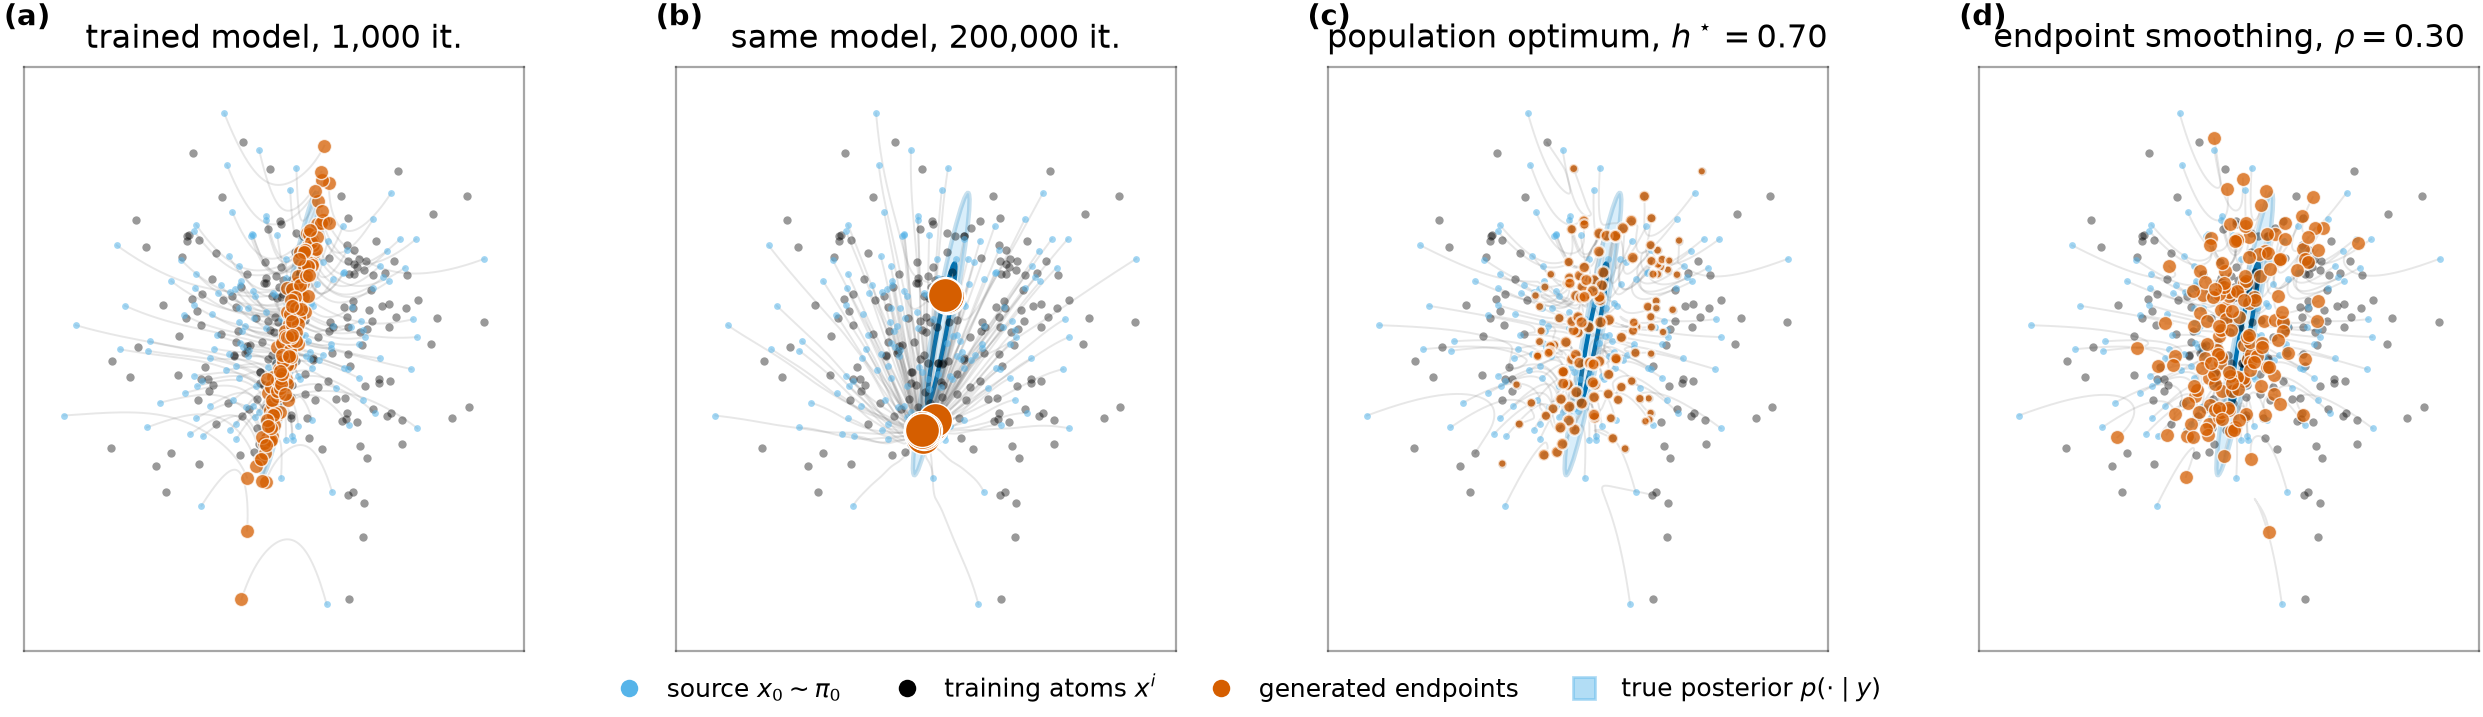
\includegraphics[width=0.88\textwidth]{fig_flow_portrait.png}
\caption{The mechanism in trajectory space, on one condition of the real EXP-1 instance
($d{=}2$, $N{=}200$): $160$ draws of $x_0$, the paths they follow, where they land.
(a,~b) one \emph{trained} network at two checkpoints---a posterior sampler at $1000$
iterations, sending $96\%$ of its paths to the identified atom by $200000$
(Proposition~\ref{prop:collapse}), so this is an optimiser collapsing and not only a
limit. (c) the population optimum at the $h^\star$ where $\tr\Covh=\tr\Sigmapost$
\emph{exactly}: marker area is Theorem~\ref{thm:endpoint}'s weight $p_i^{(h)}$, the
variance is right and the law is still atomic, with a floor no $h$ removes
(Proposition~\ref{prop:atomicity}); that panel is this paper's title. (d) only moving
the support leaves the atoms (Proposition~\ref{prop:tgtnoise}).
Figures~\ref{fig:traintraj} and~\ref{fig:interventions} add the checkpoints in between,
and the interventions that do not help.}
\label{fig:mechanism}
\end{figure}

In one line: \emph{conditional collapse is the zero-bandwidth limit of a
kernel-weighted empirical conditional flow}, and the natural remedy moves along that
limit without ever leaving the training atoms (Figure~\ref{fig:mechanism}). Each
population result is a short Bayes computation on a Gaussian interpolant once the object
to compute has been identified; the weight sits on that object---an exact conditional
reference law where the literature has had approximations---and on what it buys: a way
to tell a model that has recovered the posterior's second moment from one that has
recovered the posterior, a proof that two of the three interventions practitioners reach
for cannot help, and a protocol that catches an agreement statistic certifying nothing.
Section~\ref{sec:scope} marks the scope line: the theory characterises the exact
population minimiser for the empirical data law, not what a finite network trained by SGD
attains, so quantities it does not determine are reported as empirical findings, never as
predictions.

% ==========================================================================
\section{Setup and notation}
\label{sec:setup}

Fix a training set $\D=\{(x^i,y^i)\}_{i=1}^N$ with $x^i\in\R^d$, $y^i\in\R^k$,
empirical joint law $\rhohat_{XY}$ and marginal $\rhohat_X=\frac1N\sum_i\delta_{x^i}$.
Draw $I\sim\mathrm{Unif}\{1,\dots,N\}$, $X_0\sim\pi_0=\N(0,I_d)$,
$t\sim\mathrm{Unif}(0,1)$ and, when $h>0$, $\varepsilon\sim\N(0,I_k)$, independently.
Set $X_1=x^I$ and $X_t=(1-t)X_0+tX_1$ with $U:=\dot X_t=X_1-X_0$. The smoothed label is
$\widetilde Y=y^I+h\varepsilon$ with Gaussian kernel
$K_h(u)=(2\pi h^2)^{-k/2}\exp(-|u|^2/2h^2)$, and the objective is
\begin{equation}
L_h(v)=\E\big[\,|U-v(X_t,t,\widetilde Y)|^2\,\big],
\label{eq:objective}
\end{equation}
written $L_0$ when $h=0$ and $\widetilde Y=Y=y^I$.

\begin{assumption}[Standing]
\label{as:standing}
\emph{(i)} $\D$ is fixed: the expectation in \eqref{eq:objective} is over
$(I,X_0,t,\varepsilon)$ only. \emph{(ii)} The interpolant is the deterministic linear one
above, unless a noisy one is introduced explicitly. \emph{(iii)} Labels identify:
$y^i\neq y^j$ for $i\neq j$, so $Y=y^i$ determines $I=i$ at $h=0$.
\end{assumption}

Let $\bar x=\frac1N\sum_i x^i$ and
$\Xhat=\frac1N\sum_i(x^i-\bar x)(x^i-\bar x)^\top$. In the linear-Gaussian instance used
experimentally, $y=Ax+\eta$ with $\eta\sim\N(0,\sigma_{\mathrm{obs}}^2I_k)$, giving a
Gaussian analytic posterior with covariance $\Sigmapost$.

% ==========================================================================
\section{Theory}
\label{sec:theory}

\emph{Scope marker.} Everything here is under Assumption~\ref{as:standing} and
characterises the exact population minimiser over $L^2$-measurable vector fields for the
empirical data law, with $\D$ \emph{fixed}; Propositions~\ref{prop:expansion}
and~\ref{prop:nwrate} are the deliberate exception, relaxing (i) to a random design
under Assumption~\ref{as:design} and asymptotic in $N$. All proofs, and three
conventions they rely on, are in Appendix~\ref{app:proofs}. The projection identity
underlying everything is the standard $L^2$ decomposition behind every flow-matching
objective \citep{lipman2023flow,albergo2023building,liu2023rectified}.

\begin{proposition}[$L^2$ projection]
\label{prop:projection}
For every square-integrable $v$,
$L_h(v)=\E[\Var(U\mid X_t,t,\widetilde Y)]+\E\,|v-\E[U\mid X_t,t,\widetilde Y]|^2$,
so the a.e.-unique minimiser is $\vstar(x,t,y)=\E[U\mid X_t=x,t,\widetilde Y=y]$ with
$\inf_v L_h=\E[\Var(U\mid X_t,t,\widetilde Y)]$. \proofin
\end{proposition}

Lemmas~\ref{lem:cov} and~\ref{lem:wellposed} (appendix) make the conditional
expectations legitimate and the flows well posed with no additional assumption: for
$t<1$ the map $X_0\mapsto X_t$ is an invertible affine change of variables with
everywhere-positive conditional density, and every field below is locally Lipschitz on
$\R^d\times[0,1)$, so endpoint laws are well-defined weak limits
$p_1=\lim_{t\uparrow1}p_t$.

\subsection{Hard conditioning: exact collapse}
\label{sec:theory-hard}

What does the conditional expectation of Proposition~\ref{prop:projection} collapse to
once the conditioning event pins down a single index?

\begin{proposition}[Exact conditional collapse; $h=0$]
\label{prop:collapse}
Let $h=0$. Then
(a) $v_0^\star(x,t,y^i)=(x^i-x)/(1-t)$ for $t<1$;
(b) $\inf_v L_0(v)=0$;
(c) the ODE $\dot x_t=(x^i-x_t)/(1-t)$ has the explicit solution
$x_t=(1-t)x_0+tx^i$, so $x_t\to x^i$ for every $x_0$; and
(d) $p_1^{\mathrm{cond}}(\cdot\mid y^i)=\delta_{x^i}$, hence
$\Cov[p_1^{\mathrm{cond}}(\cdot\mid y^i)]=0$. \proofin
\end{proposition}
If labels are not distinct, collapse is onto the label's empirical conditional
support $|\mathcal I_y|^{-1}\sum_{i\in\mathcal I_y}\delta_{x^i}$, a single atom exactly
when the label is an identifier. The unconditional minimiser, by contrast, mixes all $N$
atoms with spatial weights $q_i(x,t)\propto\pi_0(\tfrac{x-tx^i}{1-t})$ and reaches
$\rhohat_X$ (Proposition~\ref{prop:uncond}, appendix).

\begin{corollary}[The correct conditional/unconditional distinction]
\label{cor:distinction}
Both exact population flows are supported on the training set:
$p_1^{\mathrm{cond}}(\cdot\mid y^i)=\delta_{x^i}$ and
$p_1^{\mathrm{unc}}=\frac1N\sum_i\delta_{x^i}$. The distinction is therefore not
``memorises vs.\ does not'' but \emph{single-example} vs.\
\emph{full-empirical-measure} memorisation, with observable difference in the
conditional second moment:
\begin{equation}
\Cov[p_1^{\mathrm{cond}}(\cdot\mid y^i)]=0
\qquad\text{vs.}\qquad
\Cov[p_1^{\mathrm{unc}}]=\Xhat.
\label{eq:distinction}
\end{equation} \proofin
\end{corollary}

The often-cited observation $\tr\Cov\approx\tr\Xhat$ for the unconditional baseline is
precisely \eqref{eq:distinction}: evidence of full-empirical-measure memorisation,
\emph{not} of non-memorisation. Two empirical findings read the same way---that verbatim
replication is common with text conditioning, rare without it, and mitigated by
randomising captions \citep{somepalli2023copying}, and that \emph{uninformative random}
labels sharply increase memorisation \citep{gu2023memorization}---since
Proposition~\ref{prop:collapse} says informativeness is irrelevant and identification is
everything (Appendix~\ref{app:adv} tests this directly).

\subsection{Label smoothing is exactly kernel regression}
\label{sec:theory-kernel}

The natural fix for a label that identifies its example too precisely is to blur it,
replacing $y^i$ by $\widetilde Y=y^i+h\varepsilon$; the population minimiser then becomes
exactly the velocity field of a Nadaraya--Watson regression over the atoms.

\begin{proposition}[Kernel-weighted population minimiser]
\label{prop:kernel-field}
For $h>0$, $t<1$,
\begin{equation}
\vstar(x,t,y)=\sum_i w_i^{(h)}(x,t,y)\,\frac{x^i-x}{1-t},\quad
w_i^{(h)}=\frac{\pi_0\!\big(\tfrac{x-tx^i}{1-t}\big)K_h(y-y^i)}
{\sum_j\pi_0\!\big(\tfrac{x-tx^j}{1-t}\big)K_h(y-y^j)}.
\label{eq:kernel-field}
\end{equation} \proofin
\end{proposition}
This factorises the index posterior into a spatial source-consistency term and a label
kernel. With $p_i^{(h)}(y):=K_h(y-y^i)/\sum_j K_h(y-y^j)$ the normalised label weights,
Lemma~\ref{lem:mixture-coupling} identifies $\vstar$ with the conditional velocity of the
coupling $I\sim p^{(h)}(y)$, $X_1=x^I$, which gives the endpoint law.

\begin{theorem}[Endpoint law under label smoothing]
\label{thm:endpoint}
For every $h>0$ and query $y$,
\begin{equation}
p_h^{\mathrm{gen}}(\cdot\mid y)=\sum_{i=1}^N p_i^{(h)}(y)\,\delta_{x^i}.
\label{eq:endpoint}
\end{equation} \proofin
\end{theorem}
\begin{corollary}[Zero bandwidth at fixed $N$]
\label{cor:zerobw}
If $y$ has a unique nearest label $i^\star=\arg\min_i|y-y^i|$, then
$p_i^{(h)}(y)\to\mathbf 1\{i=i^\star\}$ as $h\to0$, so
$p_h^{\mathrm{gen}}(\cdot\mid y)\Rightarrow\delta_{x^{i^\star}}$; at $y=y^i$ this
recovers Proposition~\ref{prop:collapse}. \proofin
\end{corollary}
\begin{corollary}[Infinite bandwidth at fixed $N$]
\label{cor:infbw}
$p_i^{(h)}(y)\to1/N$ for every $i$ as $h\to\infty$, so
$p_h^{\mathrm{gen}}(\cdot\mid y)\Rightarrow p_1^{\mathrm{unc}}$. \proofin
\end{corollary}
So $h$ interpolates continuously between the two hard regimes of
Section~\ref{sec:theory-hard}.

\begin{proposition}[Exact finite-$N$ moments]
\label{prop:moments}
$\bar x_h(y)=\sum_i p_i^{(h)}(y)\,x^i$ and
$\Covh(y)=\sum_i p_i^{(h)}(y)\,(x^i-\bar x_h(y))(x^i-\bar x_h(y))^\top$, both exactly
computable from the training set for any $h$, and the correct reference against which
generated moments must be compared. $\tr\Covh(y)$ need not be monotone in $h$. \proofin
\end{proposition}

These are the moments of the law identified by Theorem~\ref{thm:endpoint}, and the
object every experiment below measures against. For labels \emph{close but not equal},
Proposition~\ref{prop:nearduplicate} shows a usable bandwidth exists exactly when
clusters are tight relative to their separation, and that inside that window
$n_{\mathrm{eff}}$ counts the cluster rather than the dataset: near-duplicate labels buy
effective sample size, not continuity.

\begin{proposition}[Label smoothing never leaves the training set]
\label{prop:atomicity}
For every $h\in[0,\infty)$, $\operatorname{supp}(p_h^{\mathrm{gen}}(\cdot\mid y))
\subseteq\{x^1,\dots,x^N\}$. Consequently, if the true posterior $p(\cdot\mid y)$ is
absolutely continuous,
\begin{equation}
W_2^2\big(p_h^{\mathrm{gen}}(\cdot\mid y),\,p(\cdot\mid y)\big)\ \ge\
\int\operatorname{dist}\big(x,\{x^i\}\big)^2\,p(x\mid y)\,dx\ >\ 0,
\label{eq:w2floor}
\end{equation}
\emph{and this lower bound does not depend on $h$.} \proofin
\end{proposition}
This is the central caveat on any ``variance is restored at $h\approx0.1$'' claim:
label smoothing redistributes weight over training atoms and never generates new
samples, so matching $\tr\Covh$ matches a second moment, not the posterior. A genuine
remedy needs $h\to0$ \emph{and} $N\to\infty$ jointly (Proposition~\ref{prop:nwrate}),
not $h$ alone. The floor's \emph{size} decides whether this matters, and it is governed
by the rate factor $N^{-1/d}$: $0.071$ at our $(d,N)=(2,200)$ default but $0.9975$ at
$(3072,2000)$. Zador's theorem \citep[Ch.~6]{graf2000quantization} gives that rate for
the \emph{optimal} $N$-point quantiser and so bounds the floor from below; whether
i.i.d.\ atoms attain it is measured in Appendix~\ref{app:deferred}, where the
obstruction is negligible exactly where it is easy to measure and stays large relative
to the posterior scale in the image-dimensional regime.

\subsection{Escaping the obstruction: smoothing the endpoint}
\label{sec:theory-remedy}

Proposition~\ref{prop:atomicity} rules out any remedy leaving the endpoint law on the
training atoms---label smoothing, and trivially the interpolant noise of
Section~\ref{sec:theory-noise} since $\gamma(1)=0$---and says what a remedy must do:
move the support. Of the three places to inject noise (label, path, endpoint), only
the third does.

\begin{proposition}[Endpoint smoothing]
\label{prop:tgtnoise}
Replace the endpoint by $X_1=x^I+\rho\,\xi$ with $\xi\sim\N(0,I_d)$ independent of
$(I,X_0,\varepsilon)$ and redrawn every step, keeping label bandwidth $h\ge0$. Write
$s_t^2=(1-t)^2+t^2\rho^2$. Then $\vstar$ is again a weighted average of per-atom
fields, now with spatial weights $\varphi_{s_t}(x-tx^i)$ in place of
$\pi_0(\tfrac{x-tx^i}{1-t})$ (explicitly, \eqref{eq:tgtfield} in the appendix), and
the endpoint law is
\begin{equation}
p_1(\cdot\mid y)=\sum_i p_i^{(h)}(y)\,\N(x^i,\rho^2I_d),
\qquad
\bar x=\bar x_h(y),\quad \Cov=\Covh(y)+\rho^2I_d.
\label{eq:tgtendpoint}
\end{equation}
For every $\rho>0$ this law is absolutely continuous, so \eqref{eq:w2floor} does not
apply to it; moreover $s_1=\rho>0$, so $\vstar$ extends continuously to $t=1$ and the
$1/(1-t)$ blow-up of $(\star)$ disappears. \proofin
\end{proposition}

Two caveats, both quantified in Section~\ref{sec:exp1}: removing a lower bound is not
reducing the distance, since \eqref{eq:tgtendpoint} is a kernel density estimate paying
$+\rho^2I_d$ of variance for its continuity, and the gain is bounded by the obstruction
removed. As a second knob, $h$ sets $\bar x_h$ and $\Covh$ while $\rho$ shifts the
covariance, so together they match the posterior's first \emph{and} second moments with a
continuous law, where $h$ alone hits at most one.

One place in this paper leaves the fixed-$\D$ setting, to ask what $\Covh$ converges to
when the training set is itself an i.i.d.\ sample and $N\to\infty$---the only regime in
which label smoothing is a genuine remedy rather than a reweighting. Under a pointwise
homoscedastic regularity hypothesis, Proposition~\ref{prop:expansion} (appendix) gives
$\Covh(y)=\Sigma(y)+h^2J(y)J(y)^\top+O(h^4)+O_P((Nh^k)^{-1/2})$, whose between-group
inflation $h^2\|J\|_F^2$ produces the over-smoothing branch of the empirical U-curve and
is a parameter-free prediction in the linear-Gaussian model, where $\mu$ is affine. It
should not be expected to describe an image model, and the across-condition slope of
$0.481$ in Section~\ref{sec:cifarddpm} is what that failure to transfer looks like.
Proposition~\ref{prop:nwrate} gives the companion Nadaraya--Watson rates for
$\bar x_h(y)$ and records why queries at $y=y^i$ are \emph{design points}, so that
$h\to0$ limit is a genuinely different one from Corollary~\ref{cor:zerobw}'s fixed-$N$
collapse---same symbol, opposite conclusions.

\subsection{Stochastic interpolant noise does not help}
\label{sec:theory-noise}

An equally natural place to inject randomness is the interpolant path itself, and
this remedy is qualitatively different: it never touches the population endpoint, at any
noise level. Replace the interpolant by $X_t=(1-t)X_0+tX_1+\gamma(t)Z$ with
$Z\sim\N(0,I_d)$ independent and $\gamma(t)=\sigma\sqrt{t(1-t)}$, so
$\gamma(0)=\gamma(1)=0$. A single $Z$ defines the whole trajectory, and the correct
pathwise-derivative target is
\begin{equation}
\dot X_t=X_1-X_0+\dot\gamma(t)Z,\qquad
\dot\gamma(t)=\frac{\sigma(1-2t)}{2\sqrt{t(1-t)}};
\label{eq:c2target}
\end{equation}
regressing on $X_1-X_0$ alone is a \emph{different} objective. Write
$s_t^2:=(1-t)^2+\gamma(t)^2=(1-t)[(1-t)+\sigma^2t]$, so $s_0=1$ and $s_1=0$.

\begin{proposition}[Closed form and endpoint invariance in $\sigma$]
\label{prop:prop17}
Let $h=0$ and $v_\sigma^\star=\E[\dot X_t\mid X_t,t,Y]$ for target
\eqref{eq:c2target}. Then for $t<1$:
(a) $v_\sigma^\star(x,t,y^i)=x^i+c(t)(x-tx^i)$ with
$c(t)=\frac{-(1-t)+\frac{\sigma^2}2(1-2t)}{s_t^2}=\frac12\frac{d}{dt}\log s_t^2$;
(b) the flow is $x_t=t\,x^i+s_t\,x_0$; and
(c) since $s_1=0$,
\begin{equation}
p_1^{\mathrm{cond}}(\cdot\mid y^i)=\delta_{x^i}\quad\text{for every }\sigma\ge0.
\label{eq:invariance}
\end{equation} \proofin
\end{proposition}

Part~(b) gives the flow in closed form and (c) follows because $s_1=0$, so no
integrator and no early stopping enter the argument: the endpoint is pinned by the
interpolant itself. The reason is structural---any admissible schedule must satisfy
$\gamma(1)=0$, since otherwise the path never reaches the data, and that is exactly the
condition erasing the noise at the endpoint, so interpolant noise is not a remedy that
happens to fail but one that cannot in principle succeed (Remark~\ref{rem:notsampler}
and Figure~\ref{fig:interpolant}, appendix).
Corollary~\ref{cor:prop18} records what it \emph{does} change---it raises the
irreducible error and halves the Lipschitz blow-up rate, neither touching $p_1$---and
Proposition~\ref{prop:factors} locates the difference: the two noises multiply different
factors of the same index posterior, and only the label factor survives to $t=1$. That
separates this mechanism from the unconditional ``resample-$x_0$'' remedy of
\citet{gradvar2025}, which operates through attainability rather than through the
population optimum.

\subsection{Classifier-free guidance does not escape either}
\label{sec:theory-cfg}

Guidance is the remedy a practitioner is most likely to reach for, and it is not covered
by Proposition~\ref{prop:prop17}; with both exact fields in closed form its endpoint law
can be read off. For the guided field
$v_w:=(1+w)\vstar(\cdot,\cdot,y)-w\,v_{\mathrm{unc}}^\star$ at weight $w\ge0$,
Proposition~\ref{prop:cfg} (appendix) shows that $v_w(x,t)=(m_w(x,t)-x)/(1-t)$ with
$m_w$ an \emph{affine} combination of the atoms, and that the trajectory's component
orthogonal to $\mathcal A:=\operatorname{aff}\{x^1,\dots,x^N\}$ obeys $q_t=(1-t)q_0$.
The guided endpoint law is therefore supported in $\mathcal A$ for every $w$ and every
initial law, so when $N\le d$ that support is Lebesgue-null and no guidance weight makes
the conditional law absolutely continuous. That is a statement about \emph{dimension},
vacuous when $N>d$; integrating the exact guided field shows more, that endpoints land on
the atoms themselves and larger $w$ changes \emph{which} atom is reached
(Proposition~\ref{prop:cfgatom}).

The four interventions therefore order themselves---inert (interpolant noise, at every
noise level), atom-preserving (guidance), reweighting (label smoothing, so the atomicity
ceiling still binds), support-moving (endpoint smoothing, at $+\rho^2I_d$ of variance)---
and that ordering is the practical content of the theory.

\subsection{What survives the flow, and what paces the collapse}
\label{sec:survival}

The results so far describe the population minimiser; none says what happens to a model
merely \emph{close} to it. Appendix~\ref{app:survivaltheory} closes that gap with a
contraction estimate. Writing $\Delta$ for a model's velocity error against $(\star)$ and
$e_t$ for its trajectory's deviation from the exact one,
Proposition~\ref{prop:survival} is the identity $e_t=(1-t)I(t)$ with
$I(t):=\int_0^t\Delta(x^v_s,s)(1-s)^{-1}ds$, from which $\lim_{t\uparrow1}e_t=e_\star$
\emph{iff} $I(t)=e_\star/(1-t)+o((1-t)^{-1})$. The collapsed field is self-enforcing: its
linear part $-\tfrac1{1-t}I_d$ contracts at a diverging rate, so an error of size
$c(1-t)^{-a}$ leaves a deviation that vanishes for $a<1$, equals exactly $c$ at $a=1$ and
is unbounded for $a>1$---a trichotomy realised by explicit fields, not merely permitted.
A model can retain conditional variance only by carrying an endpoint-scale
\emph{accumulated} error, which closes a loop the paper had open, since
Remark~\ref{lem:norepr} observes that no finite network with globally Lipschitz
activations represents $1/(1-t)$ pointwise; the converse constrains $I$ and not $\Delta$
pointwise, and we claim no pointwise version. A Lipschitz hypothesis on the \emph{error},
not on the field, converts this into the training loss: Corollary~\ref{cor:lossform}
bounds the root-mean-square deviation at truncation $1-\delta$ by
$e^{L_\Delta}\sqrt{\mathcal L_i(v)\,\delta}$, so collapse is loss-controlled in a precise
sense---the retained deviation is bounded by the loss the optimiser has not yet
removed---and stopping early is the only other lever. On EXP-1's own checkpoints that
slope is $0.485$ at $R^2=0.998$ against the predicted $\tfrac12$
(Appendix~\ref{app:survival}, where the constant is loose by $25\times$ and unused).

\subsection{Finite capacity, finite samples, and scope}
\label{sec:scope}

Two further results are kept in the appendices and \emph{not} claimed here: a loss floor
$d/(3L)$ from a uniform Lipschitz bound, some $50\times$ below the observed plateau
(Corollary~\ref{cor:floor}); and two representability results for a \emph{randomly
drawn} finite \emph{unconditional} batch (Appendix~\ref{sec:theory-d2}), which the
conditional statements do not need.

What the population theory proves are exact consequences for the empirical minimiser
(Propositions~\ref{prop:collapse}--\ref{prop:tgtnoise},
Corollaries~\ref{cor:zerobw}--\ref{cor:infbw}). It does \emph{not} determine the number
of SGD steps to approach the optimum; the dependence of \emph{observed} collapse on $N$
at fixed architecture, since the population optimum collapses for every finite $N$ and a
non-collapsing $N{=}5000$ run probes representation and optimisation instead; the
dependence on $\sigma_{\mathrm{obs}}$, where the theory implies no monotonicity; the
monotonicity of $\tr\Covh$ in $h$; or finite-sample error bars. Nothing in that second
list is called a prediction that ``matched'' or ``failed''; it is marked empirical.
\emph{The theory predicts the destination, not the speed}---a real gap, since the
phenomenon practitioners report is temporal and the question they ask is when to stop,
and a characterisation of the collapse time in $N$, $d$ and capacity is the main thing
missing here.

% ==========================================================================
\section{Experiments}
\label{sec:experiments}

\paragraph{Setup.} Unless noted, EXP-1 uses the linear-Gaussian problem
$d{=}2,\,k{=}1,\,N{=}200,\,\sigma_{\mathrm{obs}}{=}0.1$ with a 4-layer width-128 MLP,
Adam, RK4 integration stopping at $t{=}1{-}10^{-3}$, and $M{=}1000$ samples at 20
training and 8 held-out conditions; full settings are in Appendix~\ref{app:exp}. We do
\emph{not} early-stop: overtraining is the object of study. Sweeps use five seeds, and
the seed controls \emph{both} the problem instance and the training randomness, so every
error bar (a population standard deviation) mixes the two; Appendix~\ref{sec:seedsplit}
separates them and finds the instance carries $78\%$.

\subsection{Synthetic instances: the exact-theory quantities}
\label{sec:exp1}

\paragraph{EXP-1 (P1--P4).} Table~\ref{tab:exp1} and Figure~\ref{fig:p1p4} (appendix)
report the four exact-theory observables. Past the good-calibration phase the conditional
generated variance collapses from $\approx\Sigmapost$ toward $0$ (P1), the velocity field
approaches $(x^i-x)/(1-t)$ (P2), the generated mean moves from $\mu_{\mathrm{post}}$
toward $x^i$ (P3), and the unconditional baseline keeps data-scale variance (P4). The
variance tracks the true posterior up to $\sim\!10^4$ iterations---a correct Bayesian
sampler, which is exactly why early stopping works \citep{physicscfm2026}---and then
collapses, stalling near $0.40$ at $2\times10^5$; that residual is an \emph{optimisation}
gap and not a failure of Proposition~\ref{prop:collapse}, since all four observables keep
descending with the loss. Three measurements sharpen this (Appendix~\ref{app:exp4}): the
memorisation ratio of \citet{yoon2023memorization} reaches $0.650\pm0.033$ conditionally
against $0.389\pm0.032$ unconditionally from a common $\approx0.11$ baseline, so
\emph{both} flows memorise as Corollary~\ref{cor:distinction} says and the conditional
one more strongly; at held-out conditions the variance collapses as at training labels
while the distance to $\mu_{\mathrm{post}}(y)$ grows from $0.12$ to $0.87$---nearest-atom
collapse, not generalisation (Corollary~\ref{cor:zerobw}); and permuting $Y$ against $X$
leaves the collapse intact while that distance \emph{grows}, so the law tracks the
arbitrary label-to-example assignment rather than any relation between $x$ and $y$.

\label{sec:p7}%
\paragraph{Label smoothing tracks the kernel reference (P7).} This is our strongest
empirical confirmation of the theory, and it turns on using the right reference: $\Covh$,
not $\Sigmapost$. Over 20 conditions ($M{=}1000$, 5 seeds) the generated variance tracks
$\Covh$ at every bandwidth---ratio-to-kernel $=1.002\pm0.050$, $0.994\pm0.039$ and
$1.011\pm0.022$ at $h=0.05,0.1,0.5$ (Figure~\ref{fig:p7summary},
Table~\ref{tab:p7kernel})---a verification of the \emph{endpoint law}, stronger than a
velocity-field check, and the field agrees too. That $h\approx0.1$ ``perfectly
restores'' the posterior variance is a misreading: $\tr\Cov$ merely crosses $\Sigmapost$
there because $\Sigmapost\approx\Covh|_{h=0.1}$ for this problem. Three consequences
follow (Appendices~\ref{sec:aux} and~\ref{app:tgt}). The law stays atomic even at the
best-matching $h$ ($n_{\mathrm{eff}}\approx26/200$), so matching variance is not
recovering the posterior. The floor \eqref{eq:w2floor} is small here, $F=0.0353$ or
$3.5\%$ of $\tr\Sigmapost$, while the \emph{population-optimal} atomic law already scores
below the trained model in MMD---so the MMD curves are not measuring atomicity at all.
And endpoint smoothing removes the obstruction without improving the fit: the best cell
of the $(h,\rho)$ sweep is $h{=}0.5,\rho{=}0$ in both metrics.
It helps only where the atoms are sparse enough for the floor to dominate, and the gain
grows with the floor at fixed $d$ but \emph{not} across $d$ (Table~\ref{tab:floor}): like
kernel density estimation, it is defeated by dimension. Interpolant noise changes nothing,
the generated variance being $0.367\pm0.146$ against $0.372\pm0.140$ for the
mis-specified target, as \eqref{eq:invariance} predicts.

\label{sec:exp23}%
\paragraph{Beyond the Gaussian case.} \emph{EXP-2 (Gaussian mixture).} A 4-mode GMM prior with a rank-deflating linear
observation gives a genuinely \emph{bimodal} analytic posterior. Up to $\sim\!10^4$
iterations mode coverage is $1.0$ and the MMD near zero---a calibrated sampler---after
which coverage falls to $0.72$ and the MMD grows to $\sim0.25$, while the share of late
samples nearest the $x^i$-containing mode rises from $\approx0.5$ to as much as $1.000$:
selective memorisation (Figs.~\ref{fig:exp2curves} and~\ref{fig:exp23qual}).
\emph{EXP-3 (image inpainting).} Masking the lower half of $32\times32$ MNIST
($N{=}500$), over three seeds the inpainted-region pixel variance drops $\sim100\times$ by
iteration $15000$ ($0.137\pm0.021\to(1.17\pm0.12)\times10^{-3}$) and the
nearest-training-image distance falls to $(0.77\pm0.26)\times10^{-3}$: completions diverse
at iteration 200 are identical by 15000 (Fig.~\ref{fig:exp3prog}), and CIFAR-10 collapses
the same way, $0.142\to0.0087$.

\FloatBarrier

\subsection{Realistic capacity: CIFAR-10 with a 35.75M-parameter DDPM U-Net}
\label{sec:cifarddpm}

Everything above is $d\le10$ synthetic or a $0.5$M U-Net, so the standing objection is
that the mechanism is an artefact of small capacity. We repeat EXP-3 with the standard
DDPM U-Net ($35.75$M parameters) on CIFAR-10 bottom-half inpainting, $N{=}2000$,
$d{=}3072$, $k{=}1536$, $60000$ iterations at batch $128$, evaluating $48$ conditions at
$M{=}256$ samples each (Appendix~\ref{app:exp4}).

\paragraph{Hard conditioning ($h{=}0$).} $\tr\Cov$ falls from $179.1$ at iteration $500$
to $0.431$ at $60000$, a factor of $415$; all $48$ conditions have
$n_{\mathrm{eff}}=1.00$, the generated mean identifies the correct training image at
$48/48$, and the memorisation ratio is exactly $1.000$. At this scale, on real images,
the trained model does what Proposition~\ref{prop:collapse} says the population minimiser
does.

\paragraph{Label smoothing ($h>0$): the aggregate ratio is the wrong statistic.}
Table~\ref{tab:cifarddpm} reports per bandwidth both the ratio $\tr\Cov/\tr\Covh$ the
earlier sections use and the regression we argue should replace it: the OLS slope $\beta$
of $\log\tr\Cov$ on $\log\tr\Covh$ \emph{across conditions}, which
Theorem~\ref{thm:endpoint} predicts to be $1$.

\begin{figure}[!t]
\centering
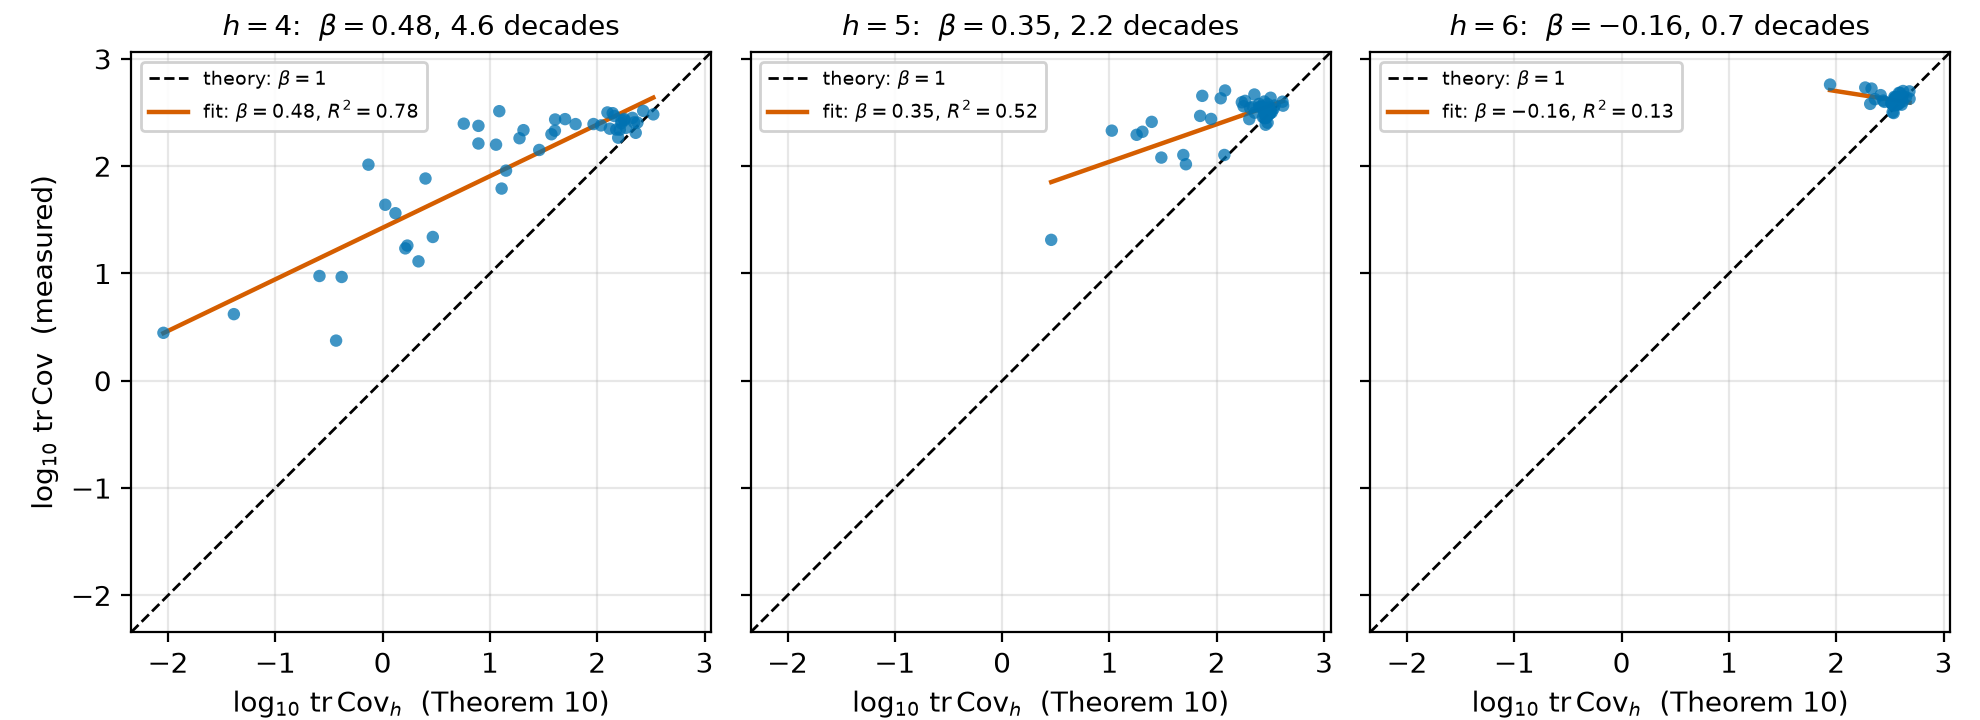
\includegraphics[width=0.58\textwidth]{fig_cifar_ddpm_tracking.png}
\caption{Measured against predicted conditional variance, per condition, on the CIFAR-10
DDPM run ($48$ conditions, $M{=}256$). Crosses: one evaluation condition each; dashed:
the identity, Theorem~\ref{thm:endpoint}'s $\beta=1$; solid: the fitted slope, with its
standard error printed in the panel. The panels share
one axis range, so the collapse of the predictor's spread---$4.57$ decades at $h{=}4$ to
$0.74$ at $h{=}6$---is visible, and the right-hand cloud sits on the identity line while
having no slope. By the level, agreement improves with $h$ (median ratio $5.30$, $1.38$,
$1.15$); by the slope, tracking disappears ($0.481$, $0.349$, $-0.156$ at $h=4,5,6$;
standard errors and bootstrap intervals in Table~\ref{tab:cifarddpm}).}
\label{fig:cifartrack}
\end{figure}

The two statistics disagree, and the disagreement is the finding. At $h{=}6$ the median
ratio is $1.15$---near-perfect agreement, by that reading---while $\beta=-0.156$ says the
model does not track the reference at all. The explanation is in the last two columns:
the reference is nearly constant across conditions ($0.74$ decades), so a ratio near $1$
is equally consistent with a model that ignores $y$. \emph{A ratio is only as informative as the variation in its
denominator}, which matters because the aggregate ratio is what the rest of the paper
reports. The informative regime is $h{=}4$, where the
reference moves over $4.57$ decades and $\beta=0.481\pm0.037$ at $R^2=0.785$: the model
preserves the ordering the theory predicts but tracks it sublinearly, recovering half of
the predicted exponent of $1$. That confirmation is partial but not static: the same slope
measured at each checkpoint (Figure~\ref{fig:betatraj}) is near zero for $8000$
iterations, then rises monotonically and is still rising when the budget ends, so
tracking is something the model \emph{learns} and $0.481$ is where $60000$ iterations
reached rather than a ceiling of the model class. It does \emph{not} establish
$\beta\to1$; three rival explanations for a fixed exponent---an additive variance floor,
a hard floor, an affine map---all lose to the power law in log space. A $35.75$M
network at $60000$ iterations is not the population minimiser: $\beta=0.481$ says how far
optimisation has come, not that the theorem fails.


\paragraph{Three supporting measurements} are in Appendix~\ref{app:exp4}: atomicity,
exact for the population minimiser, does not survive training ($38\%$ of samples are
off-atom at $h{=}6$); $n_{\mathrm{eff}}$ rather than $h$ governs the discrepancy; and
the aggregate ratio is stable only where the reference has range.

\FloatBarrier

% ==========================================================================
\section{Limitations}
\label{sec:limitations}

\paragraph{A proved property that the trained model does not inherit.}
Proposition~\ref{prop:atomicity} is exact for the object the theory describes and only
approximate for the object practitioners train, with the gap widening in $h$: the
clearest instance of the population/finite-network distinction biting, since elsewhere
the two agree in direction while here they disagree about a statement that is either
true or false. Collapse is moreover \emph{optimisation-paced}, and that gap we bound
away from one explanation rather than explain (Appendix~\ref{sec:aux}).

\paragraph{Scale, and a remedy of limited reach.} EXP-1/EXP-2 are $d\le10$ synthetic
problems and EXP-3's MNIST runs use one small U-Net; at $35.75$M parameters on CIFAR-10
hard-conditioning collapse is unambiguous but the $h>0$ agreement is only partial, so
Theorem~\ref{thm:endpoint} is confirmed there in direction and not in magnitude. Beyond
that scale, and for text-conditional label spaces carrying no natural kernel,
persistence is a claim we do not establish; endpoint smoothing's benefit is likewise
bounded by the obstruction it removes, small in exactly the regime we study most.

% ==========================================================================
\section{Conclusion}
\label{sec:conclusion}

Conditional collapse is the zero-bandwidth limit of a kernel-weighted empirical
conditional flow, and label smoothing makes that flow exact kernel regression over the
training atoms, which neither it nor interpolant noise leaves. Only endpoint smoothing
does, as far as the floor it removes is large (Appendix~\ref{app:remedies}).

\label{endmain}
\subsection*{Reproducibility statement}
All numbers reported are produced by code included in the supplementary material
(anonymized for review). Theory checks: \texttt{test\_kernel\_theory.py} (reference
table to $<0.05\%$), \texttt{analyze\_p7\_kernel.py}, \texttt{verify\_kernel\_theory.py},
\texttt{verify\_prop17.py}, \texttt{verify\_target\_noise.py},
\texttt{atomicity\_scaling.py}. Experiments: \texttt{run\_exp1.sh},
\texttt{run\_sweeps.py} ($+$\texttt{-{}-gpus N}), \texttt{train\_exp2},
\texttt{train\_exp3}, each followed by the matching analysis script. One artefact is not
regenerable from the released code as shipped: the $p7y$ runs kept their per-run metrics
but not their checkpoints, so Table~\ref{tab:p7kernel}, Table~\ref{tab:dagger} and
Figure~\ref{fig:kernel} are reproduced from those stored outputs rather than re-derived
from weights, and regenerating the checkpoints means rerunning
\texttt{run\_sweeps.py}. Proofs of all
load-bearing results are given in full in Section~\ref{sec:theory} and
Appendix~\ref{app:proofs}; every stated assumption (distinct labels, smoothness of the
weight functions, the linear-Gaussian instance) is made explicit at the point it is
used.

\subsection*{Ethics statement}
This work trains small models on synthetic linear-Gaussian and Gaussian-mixture data
and on the public MNIST and CIFAR-10 datasets. No human subjects, personally identifiable
information, or other sensitive data are used or generated. The paper's contribution
is a precise theoretical and empirical account of an existing memorisation phenomenon
in conditional generative models, which bears directly on the data-privacy and
copyright concerns around deployed diffusion/flow models raised in
Section~\ref{sec:intro}; by characterising the mechanism exactly, we aim to help
downstream work design principled mitigations rather than to facilitate
memorisation. We are not aware of any other ethical concerns raised by this
submission.

\subsection*{AI use statement}
We used a generative-AI coding and writing assistant (Claude, Anthropic) throughout
this project's development: to draft and revise manuscript text, including the
conversion of the manuscript to the ICLR format and multiple rounds of copy-editing;
to expand several of the proofs in Section~\ref{sec:theory} and
Appendix~\ref{app:proofs} from a theory memorandum into the propositions and proofs
given here; to write the training, evaluation, and analysis code in the released
repository; and to run and analyse several of the reported experiments, including
the adversarial-pairing ablation (Section~\ref{sec:adversarial}) and the
memorisation-ratio diagnostic (Section~\ref{sec:exp1}). We did not use generative AI
to select, fabricate, or embellish experimental results: every number reported is
produced by the released code from actual training runs. All AI-drafted proofs were
checked line-by-line against the underlying mathematics by the authors, and all
AI-assisted code and analysis outputs were independently verified by re-running the
experiments and cross-checking the reported statistics against the raw output
files. We take responsibility for the final content of this work, including all
text, claims, proofs, and code.

\bibliographystyle{plainnat}
\bibliography{refs}

% ==========================================================================
\appendix
\section{Deferred proofs}
\label{app:proofs}

\begin{proof}[Proof of Proposition~\ref{prop:projection}]
\mathtoolsset{showonlyrefs}
Let $\mathcal G=\sigma(X_t,t,\widetilde Y)$ and $m:=\E[U\mid\mathcal G]$.

\textbf{Step 1: split the loss.}
\begin{align}
L_h(v)&=\E|(U-m)+(m-v)|^2
  && U-v=(U-m)+(m-v)\\
&=\E|U-m|^2+\E|m-v|^2+2\,\E\langle U-m,\,m-v\rangle
  && \why{expand the square}\label{eq:pf:projection:1}
\end{align}

\textbf{Step 2: the cross term vanishes.}
\begin{align}
\E\langle U-m,\,m-v\rangle&=\E\big\langle\E[U-m\mid\mathcal G],\,m-v\big\rangle
  && \why{tower property; $m-v$ is $\mathcal G$-measurable}\\
&=0
  && \E[U-m\mid\mathcal G]=0\label{eq:pf:projection:2}
\end{align}

\textbf{Step 3: the minimiser.}
\begin{align}
L_h(v)&=\E[\Var(U\mid\mathcal G)]+\E|v-m|^2
  && \eqref{eq:pf:projection:1},\ \eqref{eq:pf:projection:2}\\
\inf_vL_h&=\E[\Var(U\mid\mathcal G)]
  && \E|v-m|^2\ge0,\ =0\iff v=m\ \text{a.e.}\\
\vstar(x,t,y)&=\E[U\mid X_t=x,t,\widetilde Y=y]
  && \why{unique a.e.\ minimiser}
\end{align}
This proves Proposition~\ref{prop:projection}.
\end{proof}

\begin{lemma}[Change of variables]
\label{lem:cov}
Fix $i$ and $t<1$. Conditionally on $I=i$, the map $X_0\mapsto X_t=(1-t)X_0+tx^i$ is an
invertible affine bijection of $\R^d$ with inverse $X_0=(X_t-tx^i)/(1-t)$; hence
$\sigma(X_t\mid I=i)=\sigma(X_0\mid I=i)$ and
\begin{equation}
p(x\mid I=i,t)=(1-t)^{-d}\,\pi_0\!\big(\tfrac{x-tx^i}{1-t}\big).
\label{eq:cov}
\end{equation}
The Jacobian factor $(1-t)^{-d}$ does not depend on $i$, so it cancels in every
posterior over $I$. Because $\pi_0$ is Gaussian, $p(x\mid I=i,t)>0$ for every $x$ and
every $t<1$.
\end{lemma}
\begin{proof}[Proof of Lemma~\ref{lem:cov}]
\mathtoolsset{showonlyrefs}
Fix $i$, $t<1$ and put $\Psi(x_0)=(1-t)x_0+tx^i$.

\textbf{Step 1: $\Psi$ is a bijection.}
\begin{align}
\det D\Psi&=(1-t)^d
  && \why{linear part is $(1-t)I_d$, invertible for $t<1$}\\
\Psi^{-1}(x)&=\frac{x-tx^i}{1-t}
  && \why{solve for $x_0$}\label{eq:pf:cov:1}\\
\sigma(X_t\mid I=i)&=\sigma(X_0\mid I=i)
  && \why{a bijection generates the same $\sigma$-algebra}
\end{align}

\textbf{Step 2: the density.}
\begin{align}
p_{X_t}(x)&=p_{X_0}\big(\Psi^{-1}(x)\big)\,|\det D\Psi|^{-1}
  && \why{change of variables}\\
&=(1-t)^{-d}\,\pi_0\!\big(\tfrac{x-tx^i}{1-t}\big)
  && \eqref{eq:pf:cov:1};\ X_0\sim\pi_0\perp I\label{eq:pf:cov:2}
\end{align}
This is \eqref{eq:cov}.

\textbf{Step 3: cancellation and positivity.}
\begin{align}
(1-t)^{-d}&\ \text{does not depend on $i$ or $x$}
  && \why{cancels in $\Pr(I=i\mid X_t=x,t)$, by \eqref{eq:pf:cov:2}}\\
p(x\mid I=i,t)&>0
  && \pi_0>0\ \text{(Gaussian)},\ \Psi^{-1}\ \text{bijective}
\end{align}
This proves Lemma~\ref{lem:cov}.
\end{proof}

\begin{lemma}[Well-posedness]
\label{lem:wellposed}
Let $w_1,\dots,w_N:\R^d\times[0,1)\to[0,1]$ be $C^\infty$ with $\sum_i w_i\equiv1$, and
set $v(x,t)=\sum_i w_i(x,t)(x^i-x)/(1-t)$ and $M=\max_i|x^i|$. Then:
\begin{enumerate}[label=(\alph*),leftmargin=2em]
\item $v\in C^\infty(\R^d\times[0,1))$, hence is locally Lipschitz in $x$, uniformly on
  compact subsets of $[0,1)$;
\item for every $x_0$ the ODE $\dot x_t=v(x_t,t)$, $x_{t=0}=x_0$, has a unique solution
  on the whole of $[0,1)$, and it obeys $|x_t|+M\le(|x_0|+M)/(1-t)$;
\item writing $\Phi_{t}$ for the resulting flow map, for every $\mu_0\in\mathcal P(\R^d)$
  the curve $\mu_t:=(\Phi_t)_\#\mu_0$ is the \emph{unique} narrowly continuous measure
  solution of $\partial_t\mu_t+\nabla\!\cdot(v\mu_t)=0$ on $[0,1)$ with initial datum
  $\mu_0$.
\end{enumerate}
We do \emph{not} claim that $\lim_{t\uparrow1}\mu_t$ exists for arbitrary such weights;
where an endpoint law is asserted below (Propositions~\ref{prop:collapse}
and~\ref{prop:kernel-field}, Theorem~\ref{thm:endpoint}) its existence is established
directly, from almost-sure convergence of the interpolant, and $p_1$ denotes that weak
limit.
\end{lemma}
\begin{proof}[Proof of Lemma~\ref{lem:wellposed}]
\mathtoolsset{showonlyrefs}
\textbf{Step 1: part (a).}
\begin{align}
v&=\sum_iw_i\,\frac{x^i-x}{1-t}\in C^\infty(\R^d\times[0,1))
  && w_i\in C^\infty,\ (x^i-x)/(1-t)\in C^\infty\\
\nabla_xv&\ \text{continuous, bounded on compacts}
  && \why{so $v$ is locally Lipschitz in $x$}
\end{align}

\textbf{Step 2: part (b).} Local existence and uniqueness on $[0,\tau)$ is
Picard--Lindel\"of \citep[Ch.~II]{hartman2002ode}, by Step~1. For the bound put $g(t)=|x_t|+M$.
\begin{align}
|v(x,t)|&\le\sum_iw_i\,\frac{|x^i-x|}{1-t}\le\frac{M+|x|}{1-t}\label{eq:vgrowth}\\
  &\quad w_i\ge0,\ \textstyle\sum_iw_i=1\\
g'(t)&\le|v(x_t,t)|\le\frac{g(t)}{1-t}\\
  &\quad g\ \text{Lipschitz, a.e.\ differentiable};\ \eqref{eq:vgrowth}\\
g(t)&\le g(0)\exp\!\int_0^t\frac{ds}{1-s}=\frac{g(0)}{1-t}\label{eq:pf:wellposed:1}\\
  &\quad \why{Gr\"onwall}
\end{align}
The right-hand side of \eqref{eq:pf:wellposed:1} is finite for every $t<1$, so the solution
cannot blow up before $t=1$: $\tau=1$.

\textbf{Step 3: part (c), existence.} For $\varphi\in C_c^\infty$ and $\mu_t=(\Phi_t)_\#\mu_0$,
\begin{align}
\frac{d}{dt}\int\varphi\,d\mu_t&=\int\nabla\varphi(\Phi_t)\cdot v(\Phi_t,t)\,d\mu_0
  && \why{chain rule along the flow}\\
&=\int\nabla\varphi\cdot v\,d\mu_t
  && \why{push-forward}\label{eq:pf:wellposed:2}
\end{align}
This is the weak form of $\partial_t\mu_t+\nabla\!\cdot(v\mu_t)=0$.

\textbf{Step 4: part (c), uniqueness.} Fix $T<1$, a narrowly continuous solution $(\mu_t)$ with
datum $\mu_0$, and $\psi(x,s):=\varphi(\Phi_{s,T}(x))$, which is $C^1$ with compact support in $x$.
\begin{align}
\partial_s\psi+v\cdot\nabla\psi&=0,\quad\psi(\cdot,T)=\varphi
  && \why{characteristics}\label{eq:pf:wellposed:3}\\
\frac{d}{ds}\int\psi(\cdot,s)\,d\mu_s&=\int(\partial_s\psi+v\cdot\nabla\psi)\,d\mu_s=0
  && \why{test the equation; \eqref{eq:pf:wellposed:3}}\label{eq:pf:wellposed:4}\\
\int\varphi\,d\mu_T&=\int\psi(\cdot,0)\,d\mu_0
  && \eqref{eq:pf:wellposed:4}\text{ from $s=0$ to $T$}\\
&=\int\varphi\,d\big((\Phi_T)_\#\mu_0\big)
  && \psi(\cdot,0)=\varphi\circ\Phi_{0,T}
\end{align}
As $\varphi$ and $T<1$ were arbitrary, $\mu_T=(\Phi_T)_\#\mu_0$. This is the classical
smooth-field case \citep[see][Ch.~8, for far weaker regularity]{ambrosio2008gradient}.
Steps~1--4 prove Lemma~\ref{lem:wellposed}.
\end{proof}

Both $v_{\mathrm{unc}}^\star$ and $\vstar$ have this form with smooth weights, so
Lemma~\ref{lem:wellposed} applies and no ``assume the flow is well defined'' hypothesis
is needed. We now give the remaining proofs in full.

\begin{proposition}[Unconditional endpoint is the full empirical law]
\label{prop:uncond}
For $L_{\mathrm{unc}}(v)=\E|X_1-X_0-v(X_t,t)|^2$ and $t<1$, with
$q_i(x,t)=\Pr(I=i\mid X_t=x,t)\propto\pi_0\!\big(\tfrac{x-tx^i}{1-t}\big)$,
\[
v_{\mathrm{unc}}^\star(x,t)=\sum_i q_i(x,t)\,\frac{x^i-x}{1-t},\qquad
p_1^{\mathrm{unc}}=\rhohat_X=\tfrac1N\sum_i\delta_{x^i}.
\]
Moreover $\inf_v L_{\mathrm{unc}}>0$ whenever $x^i\ne x^j$ for some $i\ne j$.
\end{proposition}

\begin{proof}[Proof of Proposition~\ref{prop:collapse}]
\mathtoolsset{showonlyrefs}
\textbf{Step 1: the index is pinned.}
\begin{align}
\{Y=y^i\}&=\{I=i\}
  && \why{Assumption~\ref{as:standing}(iii)}\\
X_1&=x^i
  && \why{$I=i$}\\
X_0&=\frac{x-tx^i}{1-t}
  && \why{Lemma~\ref{lem:cov}, given $X_t=x$}\label{eq:pf:collapse:1}
\end{align}

\textbf{Step 2: part (a).}
\begin{align}
U&=x^i-X_0\\
  &\quad U=X_1-X_0\\
&=x^i-\frac{x-tx^i}{1-t}\\
  &\quad \eqref{eq:pf:collapse:1}\\
&=\frac{x^i-x}{1-t}\label{eq:pf:collapse:2}\\
  &\quad \why{common denominator}\\
v_0^\star(x,t,y^i)&=\E[U\mid X_t=x,t,Y=y^i]\\
  &\quad \why{Proposition~\ref{prop:projection}}\\
&=\frac{x^i-x}{1-t}\\
  &\quad \eqref{eq:pf:collapse:2};\ U\ \text{is measurable in the conditioning}
\end{align}

\textbf{Step 3: part (b).}
\begin{align}
U-v_0^\star(X_t,t,Y)&=0\ \text{a.s.}
  && \eqref{eq:pf:collapse:2}\\
L_0(v_0^\star)&=\E|U-v_0^\star|^2=0
  && \eqref{eq:objective}\\
\inf_vL_0&=0
  && L_0\ge0
\end{align}

\textbf{Step 4: parts (c) and (d).} Along $\dot x_t=(x^i-x_t)/(1-t)$,
\begin{align}
\frac{d}{dt}\frac{x_t-x^i}{1-t}&=\frac{\dot x_t(1-t)+(x_t-x^i)}{(1-t)^2}
  && \why{quotient rule}\\
&=0
  && \dot x_t(1-t)=x^i-x_t\label{eq:pf:collapse:3}\\
x_t&=(1-t)x_0+tx^i
  && \eqref{eq:pf:collapse:3},\ x_{t=0}=x_0\\
x_t&\to x^i\quad(t\uparrow1),\ \text{for every }x_0
  && \why{coefficient of $x_0$ is $1-t\to0$}\\
p_1^{\mathrm{cond}}(\cdot\mid y^i)&=\delta_{x^i},\quad\Cov=0
  && \why{point mass}
\end{align}
This proves Proposition~\ref{prop:collapse}.
\end{proof}

\begin{proof}[Proof of Proposition~\ref{prop:uncond}]
\mathtoolsset{showonlyrefs}
\textbf{Step 1: the index posterior.}
\begin{align}
q_i(x,t)&=\frac{\frac1N(1-t)^{-d}\pi_0\big(\frac{x-tx^i}{1-t}\big)}
  {\sum_j\frac1N(1-t)^{-d}\pi_0\big(\frac{x-tx^j}{1-t}\big)}\\
  &\quad \why{Bayes; Lemma~\ref{lem:cov}}\\
&=\frac{\pi_0\big(\frac{x-tx^i}{1-t}\big)}{\sum_j\pi_0\big(\frac{x-tx^j}{1-t}\big)}\label{eq:pf:uncond:1}\\
  &\quad \why{$\frac1N(1-t)^{-d}$ does not depend on $i$}
\end{align}

\textbf{Step 2: the minimiser.}
\begin{align}
U\mid(x,t,I=i)&=\frac{x^i-x}{1-t}
  && \why{Step~2 of the proof of Proposition~\ref{prop:collapse}}\\
v_{\mathrm{unc}}^\star(x,t)&=\E[U\mid X_t=x,t]
  && \why{Proposition~\ref{prop:projection}}\\
&=\sum_iq_i(x,t)\,\frac{x^i-x}{1-t}
  && \why{tower rule over \eqref{eq:pf:uncond:1}}\label{eq:pf:uncond:2}
\end{align}

\textbf{Step 3: the endpoint law.}
\begin{align}
\text{flow of \eqref{eq:pf:uncond:2} is well posed}&\ \text{on }[0,1)\\
  &\quad \why{Lemma~\ref{lem:wellposed}: smooth weights, $\sum_iq_i=1$}\\
\mathrm{Law}(X_t)&=(\Phi_t)_\#\pi_0\\
  &\quad \why{Steps~2--3 of Theorem~\ref{thm:endpoint}, uniform law on $I$}\\
p_t&\Rightarrow\rhohat_X\\
  &\quad X_t\to X_1\ \text{a.s.},\ X_1\sim\rhohat_X\\
p_1^{\mathrm{unc}}&=\rhohat_X\\
  &\quad \why{weak limit}
\end{align}

\textbf{Step 4: the loss does not vanish.} Fix $t<1$, $x$; put $u_i=\frac{x^i-x}{1-t}$ and
$\bar u=\sum_iq_iu_i$.
\begin{align}
q_i(x,t)&>0\ \ \forall i\\
  &\quad \pi_0>0,\ \eqref{eq:pf:uncond:1}\\
x^i\ne x^j&\Rightarrow u_i\ne u_j\\
  &\quad u\ \text{is injective affine in $x^i$}\\
\Var(U\mid X_t=x,t)&=\sum_iq_i\,|u_i-\bar u|^2>0\label{eq:pf:uncond:3}\\
  &\quad \why{two distinct values with positive mass}\\
\inf_vL_{\mathrm{unc}}&=\E[\Var(U\mid X_t,t)]>0\\
  &\quad \why{Proposition~\ref{prop:projection}; \eqref{eq:pf:uncond:3} at every $(x,t)$}
\end{align}
This proves Proposition~\ref{prop:uncond}.
\end{proof}

\begin{proof}[Proof of Corollary~\ref{cor:distinction}]
\mathtoolsset{showonlyrefs}
\begin{align}
p_1^{\mathrm{cond}}(\cdot\mid y^i)&=\delta_{x^i},\quad\Cov=0
  && \why{Proposition~\ref{prop:collapse}(d)}\\
p_1^{\mathrm{unc}}&=\tfrac1N\textstyle\sum_i\delta_{x^i}
  && \why{Proposition~\ref{prop:uncond}}\\
\Cov[p_1^{\mathrm{unc}}]&=\tfrac1N\textstyle\sum_i(x^i-\bar x)(x^i-\bar x)^\top=\Xhat
  && \why{definition of $\Xhat$}\label{eq:pf:distinction:1}
\end{align}
Both laws are mixtures of point masses at training examples, hence supported on the
training set; with \eqref{eq:pf:distinction:1} this is \eqref{eq:distinction}.
This proves Corollary~\ref{cor:distinction}.
\end{proof}

\begin{proof}[Proof of Proposition~\ref{prop:atomicity}]
\mathtoolsset{showonlyrefs}
\textbf{Step 1: the support.}
\begin{align}
p_h^{\mathrm{gen}}(\cdot\mid y)&=\textstyle\sum_ip_i^{(h)}(y)\,\delta_{x^i}
  && \why{Theorem~\ref{thm:endpoint}}\\
\operatorname{supp}p_h^{\mathrm{gen}}&\subseteq\{x^1,\dots,x^N\}
  && \why{finite mixture of point masses}
\end{align}

\textbf{Step 2: a pointwise bound under any coupling $(X,X')$ of $p_h^{\mathrm{gen}}$ and $p(\cdot\mid y)$.}
\begin{align}
|X-X'|&\ge\min_i|x^i-X'|=\operatorname{dist}(X',\{x^i\})
  && X\in\{x^i\}\ \text{a.s., Step~1}\label{eq:pf:atom:1}
\end{align}

\textbf{Step 3: the floor.}
\begin{align}
\E|X-X'|^2&\ge\E\operatorname{dist}(X',\{x^i\})^2
  && \why{square and integrate \eqref{eq:pf:atom:1}}\\
&=\int\operatorname{dist}(x,\{x^i\})^2p(x\mid y)\,dx=:F(y)
  && X'\sim p(\cdot\mid y)\label{eq:pf:atom:2}\\
W_2^2(p_h^{\mathrm{gen}},p(\cdot\mid y))&\ge F(y)
  && \inf\ \text{over couplings; \eqref{eq:pf:atom:2}}
\end{align}
This is \eqref{eq:w2floor}.

\textbf{Step 4: positivity, free of $h$.}
\begin{align}
F(y)&\ \text{involves $p_h^{\mathrm{gen}}$ only through }\{x^i\}
  && \why{so it does not depend on $h$}\\
p(\{x^i\}\mid y)&=0
  && p(\cdot\mid y)\ \text{absolutely continuous}\\
F(y)&>0
  && \operatorname{dist}(\cdot,\{x^i\})>0\ \ p(\cdot\mid y)\text{-a.e.}
\end{align}
This proves Proposition~\ref{prop:atomicity}.
\end{proof}

\begin{proof}[Proof of Corollary~\ref{cor:infbw}]
\mathtoolsset{showonlyrefs}
\begin{align}
K_h(y-y^i)&=(2\pi h^2)^{-k/2}\big[1+O(h^{-2})\big]
  && \max_i|y-y^i|<\infty,\ \text{uniform in $i$}\label{eq:pf:infbw:1}\\
p_i^{(h)}(y)&=\frac{1+O(h^{-2})}{N+O(h^{-2})}
  && \why{the prefactor cancels; \eqref{eq:pf:infbw:1}}\label{eq:pf:infbw:2}\\
&\longrightarrow\frac1N\quad(h\to\infty)
  && \eqref{eq:pf:infbw:2}\\
p_1&\to\tfrac1N\textstyle\sum_i\delta_{x^i}=\rhohat_X
  && \why{Theorem~\ref{thm:endpoint}}
\end{align}
This proves Corollary~\ref{cor:infbw}.
\end{proof}

\begin{proof}[Proof of Corollary~\ref{cor:zerobw}]
\mathtoolsset{showonlyrefs}
Let $i^\star$ be the unique nearest label: $|y-y^i|>|y-y^{i^\star}|$ for $i\ne i^\star$.
\begin{align}
\frac{K_h(y-y^i)}{K_h(y-y^{i^\star})}&=\exp\Big[-\frac{|y-y^i|^2-|y-y^{i^\star}|^2}{2h^2}\Big]\\
  &\quad \why{Gaussian prefactors cancel}\\
&\xrightarrow[h\to0]{}0\label{eq:pf:zerobw:1}\\
  &\quad \why{numerator of the exponent is a positive constant}\\
p_i^{(h)}(y)&\to\mathbf 1\{i=i^\star\}\label{eq:pf:zerobw:2}\\
  &\quad \why{divide by $K_h(y-y^{i^\star})$, use \eqref{eq:pf:zerobw:1}}\\
p_h^{\mathrm{gen}}&\Rightarrow\delta_{x^{i^\star}}\\
  &\quad \why{Theorem~\ref{thm:endpoint}}
\end{align}
This proves Corollary~\ref{cor:zerobw}.
\end{proof}


\begin{proof}[Proof of Proposition~\ref{prop:kernel-field}]
\mathtoolsset{showonlyrefs}
Fix $(x,t,y)$ with $t<1$.

\textbf{Step 1: Bayes' rule for the index.}
\begin{align}
\Pr(I=i\mid X_t=x,t,\widetilde Y=y)&=\frac{\Pr(I=i)\,p(x,y\mid I=i,t)}{\sum_j\Pr(I=j)\,p(x,y\mid I=j,t)}\label{eq:bayes-index}\\
  &\quad \why{Bayes}
\end{align}

\textbf{Step 2: the two observations are conditionally independent.}
\begin{align}
X_t&=(1-t)X_0+tx^i,\quad\widetilde Y=y^i+h\varepsilon
  && \why{given $I=i$}\\
X_t\perp\widetilde Y\mid I=i
  &&& X_0\perp\varepsilon\\
p(x,y\mid I=i,t)&=(1-t)^{-d}\pi_0\big(\tfrac{x-tx^i}{1-t}\big)K_h(y-y^i)
  && \why{Lemma~\ref{lem:cov};\ density of $y^i+h\varepsilon$}\\
\Pr(I=i\mid X_t=x,t,\widetilde Y=y)&=\frac{\pi_0\big(\frac{x-tx^i}{1-t}\big)K_h(y-y^i)}{\sum_j\pi_0\big(\frac{x-tx^j}{1-t}\big)K_h(y-y^j)}
  && \eqref{eq:bayes-index}\\
&=w_i^{(h)}
  && \why{$\frac1N(1-t)^{-d}$ cancels}
\end{align}

\textbf{Step 3: the per-index target.}
\begin{align}
U\mid(X_t=x,I=i)&=\frac{x^i-x}{1-t}
  && \why{Lemma~\ref{lem:cov}; Proposition~\ref{prop:collapse}(a)}
\end{align}

\textbf{Step 4: average over the posterior.}
\begin{align}
\vstar(x,t,y)&=\E[U\mid X_t=x,t,\widetilde Y=y]
  && \why{Proposition~\ref{prop:projection}}\\
&=\sum_iw_i^{(h)}(x,t,y)\,\frac{x^i-x}{1-t}
  && \why{Steps~2 and~3}
\end{align}
This is \eqref{eq:kernel-field}, proving Proposition~\ref{prop:kernel-field}.
\end{proof}

\begin{lemma}[Equivalent mixture coupling]
\label{lem:mixture-coupling}
Fix $y$ and consider the coupling $I\sim p^{(h)}(y)$, $X_0\sim\pi_0$ (independent of
$I$), $X_1:=x^I$, with the same linear interpolant $X_t=(1-t)X_0+tX_1$. Its
conditional velocity field $\E[X_1-X_0\mid X_t=x,t]$ equals $\vstar(x,t,y)$ of
\eqref{eq:kernel-field} for every $x,t<1$.
\end{lemma}
\begin{proof}[Proof of Lemma~\ref{lem:mixture-coupling}]
\mathtoolsset{showonlyrefs}
\textbf{Step 1: the coupling's index posterior.}
\begin{align}
\Pr(I=i\mid X_t=x,t)&\propto p_i^{(h)}(y)\,(1-t)^{-d}\pi_0\big(\tfrac{x-tx^i}{1-t}\big)\\
  &\quad \why{Bayes; Lemma~\ref{lem:cov}}\\
&\propto\pi_0\big(\tfrac{x-tx^i}{1-t}\big)K_h(y-y^i)\label{eq:pf:mix:1}\\
  &\quad p_i^{(h)}\propto K_h(y-y^i);\ (1-t)^{-d}\text{ free of }i
\end{align}

\textbf{Step 2: the two posteriors coincide.}
\begin{align}
\Pr(I=i\mid X_t=x,t)&=w_i^{(h)}(x,t,y)\\
  &\quad \eqref{eq:pf:mix:1}\ \text{is the numerator of \eqref{eq:kernel-field}; both normalise over $i$}
\end{align}

\textbf{Step 3: the velocity.}
\begin{align}
\E[X_1-X_0\mid X_t=x,t]&=\sum_iw_i^{(h)}\,\frac{x^i-x}{1-t}
  && X_1-X_0=\frac{x^i-x}{1-t}\ \text{given }I=i;\ \text{Step~2}\\
&=\vstar(x,t,y)
  && \eqref{eq:kernel-field}
\end{align}
This proves Lemma~\ref{lem:mixture-coupling}.
\end{proof}

\begin{proof}[Proof of Theorem~\ref{thm:endpoint}]
\mathtoolsset{showonlyrefs}
Fix $h>0$, $y$, and let $(I,X_0,X_1,X_t)$ be the coupling of Lemma~\ref{lem:mixture-coupling}.

\textbf{Step 1: the field is the coupling's velocity.}
\begin{align}
\vstar(x,t,y)&=\E[X_1-X_0\mid X_t=x,t]
  && \why{Lemma~\ref{lem:mixture-coupling}}\\
&=\sum_iw_i^{(h)}\,\frac{x^i-x}{1-t}
  && \why{definition of }w_i^{(h)}\label{eq:pf:endpoint:1}
\end{align}

\textbf{Step 2: well-posedness on $[0,1)$.}
\begin{align}
w_i^{(h)}&\ \text{smooth, positive, $\textstyle\sum_iw_i^{(h)}=1$}\\
  &\quad \why{ratio of smooth positive terms; $\pi_0>0$ (Lemma~\ref{lem:cov})}\\
\dot x_t=\vstar&\ \text{has a unique flow $(\Phi_t)_{t<1}$}\\
  &\quad \why{Lemma~\ref{lem:wellposed}}
\end{align}

\textbf{Step 3: the flow transports $\pi_0$ to $\mathrm{Law}(X_t)$.}
\begin{align}
\partial_tp_t+\nabla\!\cdot\!\big(p_t\vstar\big)&=0,\quad p_0=\pi_0
  && \why{solved by $(\Phi_t)_\#\pi_0$ and by $\mathrm{Law}(X_t)$}\label{eq:pf:endpoint:2}\\
(\Phi_t)_\#\pi_0&=\mathrm{Law}(X_t)=:p_t
  && \why{uniqueness, Lemma~\ref{lem:wellposed}(c)}
\end{align}
(The second solves \eqref{eq:pf:endpoint:2} by superposition, using Step~1.)

\textbf{Step 4: the endpoint.}
\begin{align}
X_t&=(1-t)X_0+tx^I\longrightarrow x^I\quad\text{a.s.}
  && t\uparrow1\label{eq:pf:endpoint:3}\\
p_t&\Rightarrow\mathrm{Law}(x^I)=\textstyle\sum_ip_i^{(h)}(y)\,\delta_{x^i}
  && \eqref{eq:pf:endpoint:3}\ \text{a.s.\ implies in law}\\
p_1=\lim_{t\uparrow1}p_t&=\textstyle\sum_ip_i^{(h)}(y)\,\delta_{x^i}
  && \why{identify the weak limit, Lemma~\ref{lem:wellposed}}
\end{align}
This is \eqref{eq:endpoint}, proving Theorem~\ref{thm:endpoint}.
\end{proof}


\begin{proof}[Proof of Proposition~\ref{prop:moments}]
\mathtoolsset{showonlyrefs}
\textbf{Step 1: moments of a finite mixture.}
\begin{align}
\bar x_h(y)&=\textstyle\sum_ip_i^{(h)}(y)\,x^i\\
  &\quad \why{mean of $\sum_ip_i^{(h)}\delta_{x^i}$, Theorem~\ref{thm:endpoint}}\\
\Covh(y)&=\textstyle\sum_ip_i^{(h)}(y)(x^i-\bar x_h)(x^i-\bar x_h)^\top\label{eq:pf:moments:1}\\
  &\quad \why{covariance of the same mixture}
\end{align}
Both involve only the training set and the kernel weights, so they are exactly computable.

\textbf{Step 2: $\tr\Covh$ need not be monotone.} Take $k=d=1$, $y=0$ and pairs
$(y^i,x^i)=(0,0),(1,10),(10,0)$, so $\tr\Covh=\sum_ip_i^{(h)}(x^i-\bar x_h)^2$ by \eqref{eq:pf:moments:1}.
\begin{align}
h\to0:&\quad p^{(h)}\to(1,0,0),\ \tr\Covh\to0
  && \why{Corollary~\ref{cor:zerobw}}\\
h=2:&\quad p^{(h)}=(0.531,\,0.469,\,2{\times}10^{-6}),\ \tr\Covh=24.90
  && \why{closed form}\\
h\to\infty:&\quad p^{(h)}\to(\tfrac13,\tfrac13,\tfrac13),\ \tr\Covh\to\tr\Xhat=\tfrac{200}{9}=22.22
  && \why{Corollary~\ref{cor:infbw}}
\end{align}
A function that rises from $0$ to $24.90$ and falls to $22.22$ is not monotone. This proves
Proposition~\ref{prop:moments}.
\end{proof}

\begin{assumption}[Random design, at a query point $y$]
\label{as:design}
The pairs $(x^j,y^j)$ are i.i.d.\ with marginal label density $\rho_Y$; write
$\mu(y)=\E[X\mid Y=y]$, $\Sigma(y)=\Cov(X\mid Y=y)$, $J(y)=\partial\mu/\partial y$ and
$m_4(y)=\E[\|X\|^4\mid Y=y]$. Fix $y$ in the interior of $\operatorname{supp}(\rho_Y)$
and a ball $B(y,r)$ contained in that interior. On $B(y,r)$:
\begin{enumerate}[label=(\roman*),leftmargin=2em,itemsep=1pt]
\item $\rho_Y$ is positive and $C^2$;
\item $\mu$ is $C^3$, with $M_3:=\sup_{B(y,r)}\|\nabla^3\mu\|<\infty$;
\item $\Sigma(\cdot)$ is \emph{constant} (homoscedasticity);
\item $m_4$ is bounded.
\end{enumerate}
Globally, $\rho_Y$ is bounded and $|\mu(y')|+\|\Sigma(y')\|+m_4(y')\le C(1+|y'|^m)$ for
some $C,m$.
\end{assumption}

Item~(iv) is not implied by (i)--(iii): those bound the conditional mean and covariance,
whereas $\Covh$ is a quadratic functional of $X$ whose \emph{variance} is what the
stochastic term must control. It is the hypothesis the standard kernel-smoothing rate
assumes, and Step~5 below is the only place it is used.

\begin{proposition}[Bandwidth expansion of the conditional covariance; random design]
\label{prop:expansion}
Under Assumption~\ref{as:design}, pointwise at $y$, as $Nh^k\to\infty$ and $h\to0$,
\begin{equation}
\Covh(y)=\Sigma(y)+h^2 J(y)J(y)^\top+O(h^4)+O_P\big((Nh^k)^{-1/2}\big),
\label{eq:expansion}
\end{equation}
so $\tr\Covh(y)=\tr\Sigma(y)+h^2\|J(y)\|_F^2+\cdots$. Homoscedasticity is load-bearing rather than cosmetic, the expansion is
pointwise rather than uniform in $y$, and both the regularity budget and a
heteroscedastic counterexample are discussed in Appendix~\ref{app:proofs}.
\end{proposition}

\begin{proof}[Proof of Proposition~\ref{prop:expansion}]
\mathtoolsset{showonlyrefs}
Write $\rho_Y$ for the density of $Y$ and $s(y):=\nabla\log\rho_Y(y)$, well defined since
$\rho_Y>0$ is $C^2$ near $y$.

\textbf{Step 1: reduce to a tilted population identity.} With
$q_h(y')\propto K_h(y-y')\rho_Y(y')$ and $\E_h[f]:=\E[K_h(y-Y)f]/\E[K_h(y-Y)]$ (that is,
$Y\sim q_h$, $X\mid Y$ unchanged),
\begin{align}
\Covh(y)&\longrightarrow\Cov_h^{\mathrm{pop}}(y):=\Cov_h[X]\quad(N\to\infty)\\
  &\quad \why{LLN for both weighted sums, then Slutsky}\\
\Cov_h^{\mathrm{pop}}(y)&=\E_h[\Sigma(Y)]+\Cov_h[\mu(Y)]\label{eq:pf:expansion:2}\\
  &\quad \why{total covariance; exact for every $h>0$}\\
\Cov_h^{\mathrm{pop}}(y)&\overset{?}{=}\Sigma(y)+h^2J(y)J(y)^\top+O(h^4)\label{eq:pf:expansion:1}\\
  &\quad \why{the claim, proved in Steps~3--4}
\end{align}
The discrepancy between $\Covh$ and $\Cov_h^{\mathrm{pop}}$ is the $O_P$ term of Step~5.

\textbf{Step 2: the tilted law of $u=(Y-y)/h$.} Substitute $y'=y+hu$ and $K_h(y-y')=h^{-k}\varphi(u)$.
\begin{align}
\int K_h(y-y'')\rho_Y(y'')\,dy''&=\int\varphi(u)\,\rho_Y(y+hu)\,du
  && y'=y+hu\\
\rho_Y(y+hu)&=\rho_Y(y)\big[1+h\,s^\top u+O(h^2)\big]
  && C^2\ \text{Taylor}\\
\int\varphi\,\rho_Y(y+h\cdot)&=\rho_Y(y)\big[1+O(h^2)\big]
  && \textstyle\int\varphi(u)u\,du=0\\
\tilde q_h(u)&=\varphi(u)\big[1+h\,s^\top u+O(h^2)\big]
  && \why{ratio of the two lines above}\label{eq:pf:expansion:3}
\end{align}
Use $\E_\varphi[u]=0$, $\E_\varphi[uu^\top]=I_k$, $\E_\varphi[u_au_bu_c]=0$ and
$\E_\varphi[u_au_bu_cu_d]=\delta_{ab}\delta_{cd}+\delta_{ac}\delta_{bd}+\delta_{ad}\delta_{bc}$ in
\eqref{eq:pf:expansion:3}:
\begin{align}
\E_{\tilde q_h}[u]&=h\,\E_\varphi[uu^\top]s+O(h^2)=h\,s(y)+O(h^2)\label{eq:pf:expansion:4}\\
  &\quad \why{first-order term}\\
\E_{\tilde q_h}[uu^\top]&=I_k+h\,\E_\varphi[uu^\top(s^\top u)]+O(h^2)=I_k+O(h^2)\label{eq:pf:expansion:5}\\
  &\quad \why{odd moments vanish}\\
\Cov_{\tilde q_h}[u]&=\E[uu^\top]-\E[u]\E[u]^\top=I_k+O(h^2)\label{eq:pf:expansion:6}\\
  &\quad \eqref{eq:pf:expansion:4},\ \eqref{eq:pf:expansion:5}
\end{align}

\textbf{Step 3: the within-group term.} Homoscedasticity is used here, and only here.
\begin{align}
\E_h[\Sigma(Y)]&=\E_{\tilde q_h}[\Sigma(y+hu)]\\
  &\quad Y=y+hu\\
&=\Sigma(y)+O\big(e^{-r^2/4h^2}\big)\\
  &\quad \Sigma\equiv\Sigma(y)\ \text{on $B(y,r)$; mass outside is a Gaussian tail (Step~4)}\\
&=\Sigma(y)+O(h^4)\\
  &\quad \why{$e^{-r^2/4h^2}=o(h^p)$ for all $p$}
\end{align}
Without homoscedasticity, for $\Sigma\in C^2$, the same substitution gives
\begin{align}
\E_h[\Sigma(Y)]&=\Sigma+h\,\nabla\Sigma\!\cdot\!\E[u]+\tfrac{h^2}2\nabla^2\Sigma\!\cdot\!\E[uu^\top]+o(h^2)\\
  &\quad \why{Taylor}\\
&=\Sigma+h^2\big[\nabla\Sigma\!\cdot\!s+\tfrac12\tr\nabla^2\Sigma\big]+o(h^2)\\
  &\quad \eqref{eq:pf:expansion:4},\ \eqref{eq:pf:expansion:5}
\end{align}
The bracket is $O(1)$ times $h^2$, the order of $h^2JJ^\top$, so $\|J\|_F^2$ is then not identifiable
from $\tr\Covh$. Concretely, $k=d=1$, $Y\sim\mathrm{Unif}(-2,2)$, $X\mid Y=y\sim\N(0,1+y^2)$:
\begin{align}
\mu&\equiv0,\ J\equiv0
  && \why{by construction}\\
\Covh(y)&=\E_{\tilde q_h}[1+(y+hu)^2]=\Sigma(y)+h^2
  && \why{$\rho_Y$ constant near $y$, up to tails}
\end{align}
where \eqref{eq:pf:expansion:1} with $J=0$ would predict $\Sigma(y)+O(h^4)$.

\textbf{Step 4: the between-group term.}
\begin{align}
\int_{|u|>r/h}(1+|y+hu|^{2m})\varphi(u)\,du&\le C''e^{-r^2/4h^2}\\
  &\quad \why{Gaussian tail beats the polynomial growth}\\
&=o(h^p)\ \ \forall p\\
  &\quad \why{work on $|u|\le r/h$, where $y+hu\in B(y,r)$}
\end{align}
There, $\mu\in C^3$ with $\|\nabla^3\mu\|\le M_3$ (the only use of $C^3$: $C^2$ gives $o(h^2)$, too weak):
\begin{align}
\mu(y+hu)&=\mu(y)+hJu+\tfrac{h^2}2Q(u)+R_h(u),\quad Q(u)_a=\textstyle\sum_{b,c}\partial^2_{bc}\mu_a(y)u_bu_c\\
  &\quad \why{Taylor, Lagrange remainder}\\
|R_h(u)|&\le\tfrac{M_3}6h^3|u|^3\\
  &\quad \|\nabla^3\mu\|\le M_3\\
\Cov(hJu,R_h)&=O(h^4)\\
  &\quad \why{moments of $\tilde q_h$ bounded, $h\le1$}\\
\Cov(\tfrac{h^2}2Q,R_h)&=O(h^5)\\
  &\quad \why{same}\\
\Cov[R_h]&=O(h^6)\\
  &\quad \why{same}
\end{align}
The three remainder terms are absorbed in $O(h^4)$, so:
\begin{align}
\Cov_h[\mu(Y)]&=\Cov_{\tilde q_h}\big[hJu+\tfrac{h^2}2Q(u)\big]+O(h^4)\\
  &\quad \why{drop $R_h$; covariance ignores $\mu(y)$}\\
&=h^2J\,\Cov[u]\,J^\top+h^3\big[J\,\Cov(u,Q)+\mathrm{sym}\big]+h^4\Cov[Q]\label{eq:pf:expansion:7}\\
  &\quad \why{bilinearity}\;+O(h^4)\\
h^2J\,\Cov[u]\,J^\top&=h^2JJ^\top+O(h^4)\\
  &\quad \eqref{eq:pf:expansion:6}\\
\E_{\tilde q_h}[u_au_bu_c]&=h\big[s_c\delta_{ab}+s_b\delta_{ac}+s_a\delta_{bc}\big]+O(h^2)\\
  &\quad \eqref{eq:pf:expansion:3};\ \E_\varphi[u_au_bu_c]=0\\
\Cov(u,Q(u))&=O(h)\\
  &\quad \why{every third moment is $O(h)$; $Q$ is quadratic}\\
h^3\,\Cov(u,Q(u))&=O(h^4),\qquad h^4\Cov[Q]=O(h^4)\\
  &\quad \why{previous line; trivially}\\
\Cov_h[\mu(Y)]&=h^2JJ^\top+O(h^4)\\
  &\quad \eqref{eq:pf:expansion:7}
\end{align}
Substituting Step~3 and this into \eqref{eq:pf:expansion:2} proves \eqref{eq:pf:expansion:1}.

\textbf{Step 5: the Monte-Carlo fluctuation.} Put $S_N=\frac1N\sum_jK_h(y-y^j)$,
$T_N=\frac1N\sum_jK_h(y-y^j)x^j$, so $\bar x_h=T_N/S_N$.
\begin{align}
\Var\big(K_h(y-Y)\big)&=\Theta(h^{-k})\\
  &\quad \why{height $\Theta(h^{-k})$ on volume $\Theta(h^k)$; dominates the squared mean $\Theta(1)$}\\
\Var\big(K_h(y-Y)X\big),\ \Var\big(K_h(y-Y)XX^\top\big)&=\Theta(h^{-k})\\
  &\quad m_4\ \text{bounded near $y$: the only use of (iv)}\\
S_N,\ T_N&=\E[\,\cdot\,]+O_P\big(\sqrt{h^{-k}/N}\big)\\
  &\quad \why{i.i.d.\ averages; relative error }O_P((Nh^k)^{-1/2})\\
\bar x_h&=\E_h[X]+O_P\big((Nh^k)^{-1/2}\big)\\
  &\quad \why{first-order Taylor (Slutsky) on $T_N/S_N$}\\
\Covh&=\Cov_h^{\mathrm{pop}}+O_P\big((Nh^k)^{-1/2}\big)\\
  &\quad \why{the same, for the quadratic functional}
\end{align}
Combining the last line with \eqref{eq:pf:expansion:1} gives \eqref{eq:expansion}.
This proves Proposition~\ref{prop:expansion}.
\end{proof}

\begin{proposition}[Nadaraya--Watson rates for the conditional mean]
\label{prop:nwrate}
Under the assumptions of Proposition~\ref{prop:expansion}, $\bar x_h(y)$ is exactly
the Nadaraya--Watson estimator of $\mu(y)$, with
\[
\mathrm{Bias}=O(h^2),\qquad \Var=O\big((Nh^k)^{-1}\big),\qquad
\mathrm{MSE}=O(h^4)+O\big((Nh^k)^{-1}\big),
\]
minimised at $h^\star\asymp N^{-1/(k+4)}$ \emph{provided the leading bias coefficient is
nonzero}. That proviso is not decorative: the rate balances $c_1h^4$ against
$c_2(Nh^k)^{-1}$ and needs $c_1,c_2>0$, with
$c_1=\tfrac14\mu_2(K)^2|b(y)|^2$ for
\begin{equation}
b(y):=\Delta\mu(y)+2\,\nabla\mu(y)^\top\nabla\log\rho_Y(y),
\label{eq:nwbiascoef}
\end{equation}
which pairs the curvature of $\mu$ with a design-density term. Affineness of $\mu$
annihilates only the first of the two: it is \emph{not} sufficient for zero bias,
because the design-density term survives. In the linear-Gaussian instance of
Section~\ref{sec:setup} we have $\mu(y)=By$ with $B=\Sigmapost A^\top/\sigma_{\mathrm{obs}}^2
=A^\top\Sigma_Y^{-1}$ (the Jacobian $J$ of Proposition~\ref{prop:expansion}) and
$\rho_Y=\N(0,\Sigma_Y)$, $\Sigma_Y=AA^\top+\sigma_{\mathrm{obs}}^2I_k$, so
$\Delta\mu\equiv0$ but $b(y)=-2B\Sigma_Y^{-1}y$, which is nonzero for every $y\neq0$.
There the Gaussian-kernel bias is in fact available in closed form at every $h$,
\begin{equation}
\bar x_h(y)-\mu(y)=-B\,h^2(\Sigma_Y+h^2I_k)^{-1}y=-h^2B\Sigma_Y^{-1}y+O(h^4),
\label{eq:lgbias}
\end{equation}
whose leading term is $\tfrac{h^2}2\mu_2(K)b(y)$ with $\mu_2(K)=1$, as it must be. So
the generic rate is the one our own instance exhibits, and the MSE is U-shaped in $h$
away from the origin. The exception is $y=0$, where \eqref{eq:lgbias} vanishes by
symmetry for every $h$; that is a single point, not the whole instance. Queries at $y=y^i$ are \emph{design
points}: $x^i$ receives the maximal weight $K_h(0)$, and $Nh^k\to\infty$ is exactly
what makes its relative influence vanish; without it the result does not apply there.
\end{proposition}
\begin{proof}[Proof of Proposition~\ref{prop:tgtnoise}]
\mathtoolsset{showonlyrefs}
Fix $(x,t,y)$ with $t<1$; condition on $I=i$ and put $r:=x-tx^i$.

\textbf{Step 1: the law of the interpolant.}
\begin{align}
r&=(1-t)X_0+t\rho\xi
  && X_t=(1-t)X_0+tx^i+t\rho\xi\\
r&\sim\N(0,s_t^2I_d),\quad s_t^2=(1-t)^2+t^2\rho^2
  && \why{independent Gaussians}\\
p(x\mid I=i,t)&=\varphi_{s_t}(x-tx^i)
  && \why{density of $r$}\label{eq:pf:tgtnoise:1}
\end{align}

\textbf{Step 2: the index posterior.}
\begin{align}
X_t&\perp\widetilde Y\mid I=i\\
  &\quad \why{depend on $(X_0,\xi)$ and $\varepsilon$ only; Proposition~\ref{prop:kernel-field}}\\
w_i&\propto\varphi_{s_t}(x-tx^i)\,K_h(y-y^i)\label{eq:pf:tgtnoise:2}\\
  &\quad \why{Bayes for $w_i:=\Pr(I=i\mid\cdot)$; \eqref{eq:pf:tgtnoise:1}}
\end{align}

\textbf{Step 3: the per-index target.}
\begin{align}
\Cov(X_0,r)=(1-t)I_d,&\quad\Cov(\xi,r)=t\rho I_d
  && \why{$(X_0,\xi,r)$ jointly Gaussian}\\
\E[X_0\mid r]&=\tfrac{1-t}{s_t^2}\,r,\quad\E[\xi\mid r]=\tfrac{t\rho}{s_t^2}\,r
  && \E[a\mid r]=\Cov(a,r)\Var(r)^{-1}r\label{eq:pf:tgtnoise:3}\\
\E[U\mid X_t=x,t,I=i]&=x^i+\rho\,\tfrac{t\rho}{s_t^2}r-\tfrac{1-t}{s_t^2}r
  && U=x^i+\rho\xi-X_0;\ \eqref{eq:pf:tgtnoise:3}\\
&=x^i+c_t\,(x-tx^i)
  && c_t:=\tfrac{t\rho^2-(1-t)}{s_t^2}\label{eq:pf:tgtnoise:4}
\end{align}

\textbf{Step 4: the field.}
\begin{align}
\vstar(x,t,y)&=\E[U\mid X_t=x,t,\widetilde Y=y]
  && \why{Proposition~\ref{prop:projection}}\\
&=\sum_iw_i\big[x^i+c_t\,(x-tx^i)\big]
  && \why{average \eqref{eq:pf:tgtnoise:4} over \eqref{eq:pf:tgtnoise:2}}\label{eq:tgtfield}
\end{align}

\textbf{Step 5: the endpoint law.} Take $I\sim p^{(h)}(y)$, $X_0\sim\pi_0$, $\xi\sim\N(0,I_d)$ independent,
$X_1:=x^I+\rho\xi$, same linear interpolant.
\begin{align}
\Pr(I=i\mid X_t=x,t)&\propto p_i^{(h)}(y)\,\varphi_{s_t}(x-tx^i)\propto w_i\\
  &\quad \eqref{eq:pf:tgtnoise:1};\ p_i^{(h)}\propto K_h(y-y^i)\\
\text{conditional velocity}&=\vstar\\
  &\quad \eqref{eq:pf:tgtnoise:4}\ \text{holds unchanged; Lemma~\ref{lem:mixture-coupling}}\\
(\Phi_t)_\#\pi_0&=\mathrm{Law}(X_t)\\
  &\quad \why{smooth positive weights: Lemma~\ref{lem:wellposed}; Step~3 of Theorem~\ref{thm:endpoint}}\\
\mathrm{Law}(X_t)&\Rightarrow\mathrm{Law}(x^I+\rho\xi)\\
  &\quad X_t\to X_1\ \text{a.s.}\\
&=\textstyle\sum_ip_i^{(h)}(y)\,\N(x^i,\rho^2I_d)\label{eq:pf:tgtnoise:5}\\
  &\quad \why{mixture over $I$}
\end{align}
This is \eqref{eq:tgtendpoint}.

\textbf{Step 6: moments, continuity, regularity.}
\begin{align}
\text{mean}&=\textstyle\sum_ip_i^{(h)}x^i=\bar x_h(y)\\
  &\quad \eqref{eq:pf:tgtnoise:5}\\
\Cov&=\rho^2I_d+\Covh(y)\label{eq:pf:tgtnoise:6}\\
  &\quad \why{total covariance of the mixture}\\
\text{law is absolutely continuous}&\\
  &\quad \why{each component is; so \eqref{eq:w2floor} does not apply}\\
c_t&\to1\ \ (t\uparrow1)\\
  &\quad s_1^2=\rho^2>0\\
\vstar&\ \text{bounded on bounded sets up to $t=1$}\\
  &\quad \eqref{eq:tgtfield}
\end{align}
This proves Proposition~\ref{prop:tgtnoise}.
\end{proof}

\begin{proof}[Proof of Proposition~\ref{prop:nwrate}]
\mathtoolsset{showonlyrefs}
\textbf{Step 1: classical bias and variance.} Assumption~\ref{as:design}, with $K$ bounded, symmetric,
$\int K=1$ of finite second moment, and $h\to0$, $Nh^k\to\infty$, is the standard hypothesis
of the pointwise analysis \citep[\S1.5--1.6]{tsybakov2009nonparametric}, \citep[Ch.~5]{gyorfi2002distribution}.
With $\mu_2(K)=\int u_1^2K$ and $R(K)=\int K^2$:
\begin{align}
\mathrm{Bias}&=\tfrac{h^2}2\,\mu_2(K)\,b(y)+o(h^2)\label{eq:pf:nwrate:1}\\
  &\quad \why{Taylor of $\mu(y^j)$ against symmetric weights, as in Step~4 of Proposition~\ref{prop:expansion}}\\
\Var&=\tfrac{R(K)\,\Sigma(y)}{Nh^k\rho_Y(y)}+o\big((Nh^k)^{-1}\big)\label{eq:pf:nwrate:2}\\
  &\quad \why{classical}
\end{align}
with $b$ as in \eqref{eq:nwbiascoef}. We claim no novelty for these two.

\textbf{Step 2: the optimal bandwidth.} With $c_1=\frac14\mu_2(K)^2|b(y)|^2$ and $c_2$ the constant of \eqref{eq:pf:nwrate:2},
\begin{align}
\mathrm{MSE}(h)&=c_1h^4+c_2(Nh^k)^{-1}+o(\cdot)
  && \eqref{eq:pf:nwrate:1}^2+\eqref{eq:pf:nwrate:2}\label{eq:pf:nwrate:3}\\
\tfrac{d}{dh}\mathrm{MSE}&=4c_1h^3-c_2\,k\,N^{-1}h^{-k-1}=0
  && \why{first-order condition}\\
h^{k+4}&=\tfrac{c_2k}{4c_1N},\quad h^\star\asymp N^{-1/(k+4)}
  && \why{needs $c_1,c_2>0$}\label{eq:pf:nwrate:4}\\
\tfrac{d^2}{dh^2}\mathrm{MSE}&>0\ \text{at \eqref{eq:pf:nwrate:4}}
  && \why{so it is the minimiser}
\end{align}

\textbf{Step 3: the linear-Gaussian instance.} Here $\mu(y')=By'$, $K_h=\N(0,h^2I_k)$, $\rho_Y=\N(0,\Sigma_Y)$.
\begin{align}
\bar x_h(y)&=\frac{\E[\mu(Y)K_h(y-Y)]}{\E[K_h(y-Y)]}\label{eq:pf:nwrate:5}\\
  &\quad \why{population version}\\
K_h(y-y')\rho_Y(y')&\propto\N\big(\Sigma_Y(\Sigma_Y+h^2I_k)^{-1}y,\ \cdot\big)\ \text{in }y'\label{eq:pf:nwrate:6}\\
  &\quad \why{precision }\Sigma_Y^{-1}+h^{-2}I_k,\ \text{mean }(\Sigma_Y^{-1}+h^{-2}I_k)^{-1}h^{-2}y\\
\bar x_h(y)&=B\,\Sigma_Y(\Sigma_Y+h^2I_k)^{-1}y\\
  &\quad \mu\ \text{affine: evaluate at the mean of \eqref{eq:pf:nwrate:6}}\\
\bar x_h(y)-By&=-B\,h^2(\Sigma_Y+h^2I_k)^{-1}y\label{eq:pf:nwrate:7}\\
  &\quad \Sigma_Y(\Sigma_Y+h^2I)^{-1}-I=-h^2(\Sigma_Y+h^2I)^{-1}\\
&=-h^2B\Sigma_Y^{-1}y+O(h^4)\\
  &\quad \why{expand the inverse}
\end{align}
This is \eqref{eq:lgbias}, exact at every $h$. Also $\Delta\mu=0$ and $\nabla\log\rho_Y=-\Sigma_Y^{-1}y$ give
$b(y)=-2B\Sigma_Y^{-1}y$ in \eqref{eq:nwbiascoef}. Both are checked in \texttt{scripts/verify\_nw\_bias\_affine.py}.

\textbf{Step 4: design points.} At $y=y^i$,
\begin{align}
\text{weight of $j=i$}&=\frac{K_h(0)}{\sum_jK_h(y^i-y^j)}
  && \why{definition}\\
\textstyle\sum_jK_h(y^i-y^j)&\asymp Nh^k
  && \why{in probability}\\
\text{weight}&=\Theta\big((Nh^k)^{-1}\big)\to0
  && Nh^k\to\infty
\end{align}
If $Nh^k\not\to\infty$ the weight does not vanish and the expansion does not apply, as in the fixed-$N$, $h\to0$
regime of Corollary~\ref{cor:zerobw}, where it tends to $1$. This proves Proposition~\ref{prop:nwrate}.
\end{proof}

\begin{proof}[Proof of Proposition~\ref{prop:prop17}]
\mathtoolsset{showonlyrefs}
Fix $i$; put $r:=x-tx^i$.

\textbf{Step 1: the conditional means.}
\begin{align}
r&=(1-t)X_0+\gamma(t)Z\sim\N(0,s_t^2I_d),\quad s_t^2=(1-t)^2+\gamma(t)^2\label{eq:pf:prop17:1}\\
  &\quad \why{independent Gaussians}\\
\Cov(X_0,r)=(1-t)I_d,&\quad\Cov(Z,r)=\gamma(t)I_d\\
  &\quad \gamma(t)Z\perp X_0\\
\E[X_0\mid r]&=\tfrac{1-t}{s_t^2}\,r\label{eq:pf:prop17:2}\\
  &\quad \why{$\E[a\mid r]=\Cov(a,r)\Var(r)^{-1}r$}\\
\E[Z\mid r]&=\tfrac{\gamma(t)}{s_t^2}\,r\\
  &\quad \why{same}
\end{align}

\textbf{Step 2: part (a).} By Assumption~\ref{as:standing}(iii), $Y=y^i$ pins $I=i$.
\begin{align}
v_\sigma^\star(x,t,y^i)&=\E[\dot X_t\mid X_t=x,t,I=i]
  && \why{Proposition~\ref{prop:projection}}\\
&=x^i-\E[X_0\mid r]+\dot\gamma\,\E[Z\mid r]
  && \dot X_t=x^i-X_0+\dot\gamma Z,\ \eqref{eq:c2target}\\
&=x^i+\frac{-(1-t)+\dot\gamma\gamma}{s_t^2}\,r
  && \eqref{eq:pf:prop17:2}\label{eq:pf:prop17:3}\\
\dot\gamma\gamma&=\tfrac12\tfrac{d}{dt}\gamma^2=\tfrac{\sigma^2}2(1-2t)
  && \gamma^2=\sigma^2t(1-t)\label{eq:pf:prop17:4}\\
c(t)&=\frac{-(1-t)+\frac{\sigma^2}2(1-2t)}{s_t^2}
  && \eqref{eq:pf:prop17:3},\ \eqref{eq:pf:prop17:4}\\
\tfrac{d}{dt}s_t^2&=-2(1-t)+2\dot\gamma\gamma=2s_t^2\,c(t)
  && \eqref{eq:pf:prop17:4}\\
c(t)&=\tfrac12\tfrac{d}{dt}\log s_t^2
  && \why{previous line}
\end{align}

\textbf{Step 3: part (b).} Put $u_t:=x_t-tx^i$.
\begin{align}
\dot u_t&=v_\sigma^\star(x_t,t,y^i)-x^i=c(t)\,u_t
  && \why{(a) with }r=u_t\label{eq:pf:prop17:5}\\
u_t&=u_0\exp\!\int_0^tc
  && \why{linear ODE}\\
&=x_0\exp\!\big(\tfrac12[\log s_t^2-\log s_0^2]\big)=s_t\,x_0
  && c=\tfrac12(\log s^2)';\ s_0=1,\ u_0=x_0\label{eq:pf:prop17:6}\\
x_t&=tx^i+s_tx_0
  && \why{definition of }u_t
\end{align}

\textbf{Step 4: part (c).}
\begin{align}
s_t^2&=(1-t)\big[(1-t)+\sigma^2t\big]\ \Rightarrow\ s_1=0
  && \why{definition}\\
x_t&\to x^i\quad(t\uparrow1),\ \forall x_0,\ \forall\sigma\ge0
  && \eqref{eq:pf:prop17:6}\\
p_1^{\mathrm{cond}}(\cdot\mid y^i)&=\delta_{x^i}
  && \why{point mass; this is \eqref{eq:invariance}}
\end{align}
This proves Proposition~\ref{prop:prop17}.
\end{proof}

\begin{corollary}[What interpolant noise does and does not change]
\label{cor:prop18}
Interpolant noise does not change the population endpoint law
\eqref{eq:invariance} for any $\sigma$; it \emph{does} raise the irreducible error
($\inf_v L_\sigma>0$ for $\sigma>0$, whereas $\inf_v L_0=0$) and halves the Lipschitz
blow-up rate: $\lim_{t\uparrow1}(1-t)|c(t)|=1$ for $\sigma=0$ and $\tfrac12$ for
$\sigma>0$.
\end{corollary}
\begin{proof}[Proof of Corollary~\ref{cor:prop18}]
\mathtoolsset{showonlyrefs}
\textbf{Step 1: endpoint invariance.} This is Proposition~\ref{prop:prop17}(c).

\textbf{Step 2: irreducible error, $\sigma=0$.}
\begin{align}
\gamma\equiv0&\Rightarrow\dot X_t=X_1-X_0
  && \why{the target of Proposition~\ref{prop:collapse}}\\
\inf_vL_0&=0
  && \why{Proposition~\ref{prop:collapse}(b)}
\end{align}

\textbf{Step 3: irreducible error, $\sigma>0$.} By Proposition~\ref{prop:projection}, $\inf_vL_\sigma=\E[\Var(\dot X_t\mid X_t,t,Y)]$.
With $u=(-1,\dot\gamma)$, $w=(1-t,\gamma)$: $\dot X_t-x^i=u\cdot(X_0,Z)$, $r=w\cdot(X_0,Z)$, $|w|^2=s_t^2$,
$u\cdot w=-(1-t)+\dot\gamma\gamma=c\,s_t^2$.
\begin{align}
\Var(\dot X_t\mid r,I=i)&=|u|^2-\frac{(u\cdot w)^2}{|w|^2}
  && \why{Gaussian conditioning}\\
&=\big(1+\dot\gamma^2\big)-c(t)^2s_t^2
  && \why{substitute}\label{eq:pf:prop18:1}\\
\eqref{eq:pf:prop18:1}=0&\iff u\parallel w\iff\dot\gamma(1-t)=-\gamma
  && \why{Cauchy--Schwarz equality}\label{eq:pf:prop18:2}\\
\tfrac{\sigma(1-2t)}{2\sqrt{t(1-t)}}(1-t)&=-\sigma\sqrt{t(1-t)}\iff1-2t=-2t
  && \gamma=\sigma\sqrt{t(1-t)},\ \eqref{eq:pf:prop18:2}\\
1&=0
  && \why{impossible}
\end{align}
So \eqref{eq:pf:prop18:1} is $>0$ for every $t\in(0,1)$, and $\inf_vL_\sigma>0$.

\textbf{Step 4: the Lipschitz rate.}
\begin{align}
(1-t)\,c(t)&=\frac{-(1-t)+\frac{\sigma^2}2(1-2t)}{(1-t)+\sigma^2t}
  && \why{Proposition~\ref{prop:prop17}(a)}\label{eq:pf:prop18:3}\\
&\to-1\ \ (\sigma=0),\qquad\to-\tfrac{\sigma^2/2}{\sigma^2}=-\tfrac12\ \ (\sigma>0)
  && t\uparrow1
\end{align}
This proves Corollary~\ref{cor:prop18}.
\end{proof}

\begin{proof}[Proof of Proposition~\ref{prop:factors}]
\mathtoolsset{showonlyrefs}
\textbf{Step 1: the label factor moves the endpoint.}
\begin{align}
p_h^{\mathrm{gen}}(\cdot\mid y)&=\textstyle\sum_ip_i^{(h)}(y)\,\delta_{x^i}\label{eq:pf:factors:1}\\
  &\quad \why{Theorem~\ref{thm:endpoint}; depends on $h$ only through $K_h(y-y^i)$}\\
&\Rightarrow\delta_{x^{i^\star}}\ (h\to0),\qquad\Rightarrow\rhohat_X\ (h\to\infty)\\
  &\quad \why{Corollaries~\ref{cor:zerobw}, \ref{cor:infbw}}
\end{align}
These are distinct laws (for $y$ with a unique nearest label $i^\star$), so perturbing the label factor
changes $p_1$.

\textbf{Step 2: the spatial factor does not.} Take $h=0$, any $\sigma\ge0$; $Y=y^i$ pins $I=i$ (Assumption~\ref{as:standing}(iii)).
\begin{align}
\N\big(tx^i,(1-t)^2I_d\big)&\longrightarrow\N\big(tx^i,s_t^2I_d\big)\quad\text{for every }i\label{eq:pf:factors:2}\\
  &\quad \why{interpolant noise; Lemma~\ref{lem:cov}}\\
p_1^{\mathrm{cond}}(\cdot\mid y^i)&=\delta_{x^i}\ \ \forall\sigma\\
  &\quad \why{Proposition~\ref{prop:prop17}(c), despite \eqref{eq:pf:factors:2}}
\end{align}

\textbf{Step 3: conclusion.} By Steps~1 and~2 the two mechanisms act through different, non-interchangeable
channels. This proves Proposition~\ref{prop:factors}.
\end{proof}

\begin{proof}[Proof of Proposition~\ref{prop:liplb}]
\mathtoolsset{showonlyrefs}
Let $X,X'$ be i.i.d.\ copies of $X_t\mid I=i\sim\N(tx^i,(1-t)^2I_d)$ and $e(\cdot):=f_i(\cdot,t)-v(\cdot,t,y^i)$.

\textbf{Step 1: the target's increments.}
\begin{align}
f_i(X,t)-f_i(X',t)&=-\frac{X-X'}{1-t}
  && f_i=(x^i-x)/(1-t)\\
\E|f_i(X,t)-f_i(X',t)|^2&=\frac{2(1-t)^2d}{(1-t)^2}=2d
  && X-X'\sim\N(0,2(1-t)^2I_d)\label{eq:pf:liplb:1}
\end{align}

\textbf{Step 2: the model's increments.}
\begin{align}
\E|v(X,t,y^i)-v(X',t,y^i)|^2&\le L^2\,\E|X-X'|^2
  && \why{$L$-Lipschitz}\\
&=2dL^2(1-t)^2
  && \E|X-X'|^2=2d(1-t)^2\label{eq:pf:liplb:2}
\end{align}

\textbf{Step 3: the residual's increments.}
\begin{align}
\E|e(X)-e(X')|^2&=2\E|e(X)|^2-2\big|\E e(X)\big|^2
  && X,X'\ \text{i.i.d.}\\
&\le2\,\E|e(X)|^2
  && \why{drop the mean term}\label{eq:pf:liplb:3}
\end{align}
This sharp identity, not the cruder $\E|e(X)-e(X')|^2\le4\E|e(X)|^2$, is what preserves the constant $d$.

\textbf{Step 4: the triangle inequality.}
\begin{align}
f_i(X,t)-f_i(X',t)&=[e(X)-e(X')]+[v(X,t,y^i)-v(X',t,y^i)]\\
  &\quad \why{definition of }e\\
\sqrt{2d}&\le\sqrt{2\,\E|e(X)|^2}+\sqrt{2d}\,L(1-t)\label{eq:pf:liplb:4}\\
  &\quad L^2(\Omega)\ \text{triangle};\ \eqref{eq:pf:liplb:1}\text{--}\eqref{eq:pf:liplb:3}\\
\sqrt{\E|e(X)|^2}&\ge\sqrt d\,[1-L(1-t)]_+\\
  &\quad \why{rearrange \eqref{eq:pf:liplb:4}}\\
\E|e(X)|^2&\ge d\,[1-L(1-t)]_+^2\\
  &\quad \why{square; the sign of $e$ is irrelevant}
\end{align}
This proves Proposition~\ref{prop:liplb}.
\end{proof}

\begin{proof}[Proof of Corollary~\ref{cor:floor}]
\mathtoolsset{showonlyrefs}
\textbf{Step 1: the integral.}
\begin{align}
\int_0^{1/L}(1-Ls)^2\,ds&=\Big[s-Ls^2+\tfrac{L^2s^3}3\Big]_0^{1/L}
  && \why{antiderivative}\\
&=\tfrac1L-\tfrac1L+\tfrac1{3L}=\tfrac1{3L}
  && \why{evaluate}\label{eq:pf:floor:1}
\end{align}

\textbf{Step 2: average the pointwise bound.} Proposition~\ref{prop:liplb} holds for every $i$, every
$v\in\mathcal F_L$ and every $t\in[1-1/L,1)$, where $[1-L(1-t)]_+=1-L(1-t)$.
\begin{align}
\inf_{v\in\mathcal F_L}L_0(v)&\ge d\int_{1-1/L}^1[1-L(1-t)]^2\,dt
  && \why{average over $I\sim\mathrm{Unif}$, $t\sim\mathrm{Unif}(0,1)$}\\
&=\frac d{3L}
  && s=1-t;\ \eqref{eq:pf:floor:1}\label{eq:pf:floor:2}
\end{align}
This is \eqref{eq:floor}, proving Corollary~\ref{cor:floor}.
\end{proof}

\begin{proposition}[Guidance cannot leave the affine hull of the training set]
\label{prop:cfg}
For every $w\ge0$ and $h\in[0,\infty)$, $t<1$,
\begin{equation}
v_w(x,t)=\frac{m_w(x,t)-x}{1-t},\qquad
m_w(x,t)=\sum_i\Big[(1+w)w_i^{(h)}(x,t,y)-w\,q_i(x,t)\Big]x^i,
\label{eq:cfgfield}
\end{equation}
whose coefficients sum to $1$ but are in general \emph{not} nonnegative; hence
$m_w(x,t)\in\mathcal A:=\operatorname{aff}\{x^1,\dots,x^N\}$ for every $(x,t)$. Let
$\Pi$ be the orthogonal projection onto $\mathcal A$ and $q_t:=x_t-\Pi x_t$. Then along
any solution of $\dot x_t=v_w(x_t,t)$,
\begin{equation}
q_t=(1-t)\,q_0 ,
\label{eq:cfgorth}
\end{equation}
so $q_t\to0$ and the endpoint law of the guided flow is supported in $\mathcal A$, for
every $w$ and every initial law. In particular, if $N\le d$ then $\dim\mathcal A\le
N-1<d$, so $\mathcal A$ is Lebesgue-null and \emph{no} guidance weight makes the
conditional law absolutely continuous.
\end{proposition}

\begin{proof}[Proof of Proposition~\ref{prop:cfg}]
\mathtoolsset{showonlyrefs}
\textbf{Step 1: the guided field.}
\begin{align}
\vstar&=\sum_iw_i^{(h)}\frac{x^i-x}{1-t},\qquad v_{\mathrm{unc}}^\star=\sum_iq_i\frac{x^i-x}{1-t}\label{eq:pf:cfg:1}\\
  &\quad \why{Propositions~\ref{prop:kernel-field}, \ref{prop:uncond}}\\
v_w&=(1+w)\vstar-w\,v_{\mathrm{unc}}^\star\\
  &\quad \why{definition}\\
&=\frac{m_w-x}{1-t}\\
  &\quad -(1+w)x+wx=-x;\ \text{this is \eqref{eq:cfgfield}}
\end{align}

\textbf{Step 2: $m_w$ is an affine combination of the atoms.}
\begin{align}
\textstyle\sum_i\big[(1+w)w_i^{(h)}-wq_i\big]&=(1+w)-w=1
  && \textstyle\sum_iw_i^{(h)}=\sum_iq_i=1\\
m_w(x,t)&\in\mathcal A
  && \why{coefficients sum to $1$ (not nec.\ $\ge0$)}
\end{align}

\textbf{Step 3: the orthogonal component.} $\Pi$ is affine with $\Pi z=z$ on $\mathcal A$.
\begin{align}
\dot q_t&=(I-\Pi_{\mathrm{lin}})\,\dot x_t
  && q_t=x_t-\Pi x_t\\
&=-\frac{q_t}{1-t}
  && (I-\Pi)m_w=0,\ \text{as $m_w\in\mathcal A$}\label{eq:pf:cfg:2}\\
q_t&=(1-t)\,q_0
  && \why{solve \eqref{eq:pf:cfg:2}; this is \eqref{eq:cfgorth}}
\end{align}

\textbf{Step 4: the endpoint.}
\begin{align}
\operatorname{dist}(x_t,\mathcal A)&=|q_t|=(1-t)|q_0|\to0
  && \eqref{eq:cfgorth}\\
\text{endpoint}&\in\mathcal A
  && \mathcal A\ \text{closed}
\end{align}
So the support of the endpoint law lies in $\mathcal A$.

\textbf{Step 5: well-posedness.}
\begin{align}
|m_w|&\le(1+2w)\max_i|x^i|
  && \why{Step~2: bounded coefficients}\\
|v_w|&\le\frac{(1+2w)M+|x|}{1-t}
  && \why{\eqref{eq:vgrowth} with $M\to(1+2w)M$}
\end{align}
The rest of Lemma~\ref{lem:wellposed} is unchanged. This proves Proposition~\ref{prop:cfg}.
\end{proof}

\begin{proof}[Proof of Proposition~\ref{prop:nearduplicate}]
\mathtoolsset{showonlyrefs}
Write $K_i=K_h(y-y^i)=c\,e^{-|y-y^i|^2/2h^2}$, so $p_i^{(h)}=K_i/\sum_jK_j$.

\textbf{Step 1: part (a).}
\begin{align}
\sum_{j\notin C}p_j^{(h)}&\le\frac{\sum_{j\notin C}K_j}{\sum_{i\in C}K_i}
  && \why{drop $j\notin C$ from the denominator}\\
&\le\frac{(N-|C|)\,c\,e^{-\Delta^2/2h^2}}{|C|\,c\,e^{-\varepsilon^2/2h^2}}=\eta
  && |y-y^j|\ge\Delta,\ |y-y^i|\le\varepsilon\label{eq:pf:nearduplicate:1}
\end{align}

\textbf{Step 2: part (b).} For $i,i'\in C$:
\begin{align}
\frac{p_i^{(h)}}{p_{i'}^{(h)}}&=\frac{K_i}{K_{i'}}=\exp\Big(\frac{|y-y^{i'}|^2-|y-y^i|^2}{2h^2}\Big)\\
  &\quad \why{definition}\\
&\le\exp\Big(\frac{\varepsilon^2}{2h^2}\Big)=\kappa\label{eq:pf:nearduplicate:2}\\
  &\quad |y-y^{i'}|\le\varepsilon,\ |y-y^i|\ge0
\end{align}

\textbf{Step 3: part (c).} Let $S=\sum_{i\in C}p_i^{(h)}\le1$.
\begin{align}
|C|\,p_i^{(h)}&\le\kappa S\quad(i\in C)\\
  &\quad \why{sum \eqref{eq:pf:nearduplicate:2} over $i'\in C$}\\
\sum_{i\in C}(p_i^{(h)})^2&\le S\max_{i\in C}p_i^{(h)}\le\frac{\kappa S^2}{|C|}\le\frac\kappa{|C|}\\
  &\quad \why{previous line; $S\le1$}\\
\sum_{j\notin C}(p_j^{(h)})^2&\le\Big(\sum_{j\notin C}p_j^{(h)}\Big)^2\le\eta^2\\
  &\quad \eqref{eq:pf:nearduplicate:1}\\
n_{\mathrm{eff}}=\Big(\sum_ip_i^{(h)2}\Big)^{-1}&\ge\frac{|C|}{\kappa+|C|\eta^2}\\
  &\quad \why{add the two bounds, invert}
\end{align}

\textbf{Step 4: the limits.} As $\varepsilon/h\to0$, $\Delta/h\to\infty$: $\kappa\to1$, $\eta\to0$.
\begin{align}
S&\ge1-\eta\to1\\
  &\quad \eqref{eq:pf:nearduplicate:1}\\
p_i^{(h)}/p_{i'}^{(h)}&\in[\kappa^{-1},\kappa]\to\{1\}\\
  &\quad \eqref{eq:pf:nearduplicate:2}\ \text{is symmetric in $i,i'$}\\
\text{posterior}&\to\text{uniform on $C$;\ endpoint law}\to|C|^{-1}\textstyle\sum_{i\in C}\delta_{x^i}\\
  &\quad \why{Theorem~\ref{thm:endpoint}}\\
\sum_ip_i^{(h)2}&\ge S^2/|C|,\ \text{so }n_{\mathrm{eff}}\le|C|/S^2\to|C|\\
  &\quad \why{Cauchy--Schwarz on $C$}\\
n_{\mathrm{eff}}&\to|C|\\
  &\quad \why{with the lower bound of Step~3}
\end{align}
This proves Proposition~\ref{prop:nearduplicate}.
\end{proof}

\begin{proof}[Proof of Proposition~\ref{prop:cfgatom}]
\mathtoolsset{showonlyrefs}
We are given $x_t\to x^*$, with $\dot x_t=(m_w(x_t,t)-x_t)/(1-t)$ and $m_w$ as in \eqref{eq:cfgfield}.

\textbf{Step 1: if $m_w(x_t,t)\to m^*$, then $m^*=x^*$.} Suppose $m^*\ne x^*$; put
$u=\frac{m^*-x^*}{|m^*-x^*|}$, $c=\frac{|m^*-x^*|}2>0$.
\begin{align}
\langle m_w(x_t,t)-x_t,\,u\rangle&\ge c\quad(t\ge t_0)
  && m_w-x_t\to m^*-x^*\\
\frac{d}{dt}\langle x_t,u\rangle&=\frac{\langle m_w-x_t,u\rangle}{1-t}\ge\frac c{1-t}
  && \why{the line above}\label{eq:pf:cfgatom:1}\\
\langle x_t,u\rangle&\ge\langle x_{t_0},u\rangle+c\log\tfrac{1-t_0}{1-t}\to+\infty
  && \why{integrate \eqref{eq:pf:cfgatom:1}}
\end{align}
This contradicts $x_t\to x^*$, so $m^*=x^*$.

\textbf{Step 2: both weight families concentrate on $x^{i^*}$.}
\begin{align}
\alpha_j(x,t)&=\frac{c_j\,e^{-|x-tx^j|^2/2(1-t)^2}}{\sum_lc_l\,e^{-|x-tx^l|^2/2(1-t)^2}}\label{eq:pf:cfgatom:2}\\
  &\quad \why{Lemma~\ref{lem:cov}; $c_j=K_h(y-y^j)$ for $w^{(h)}_j$, $c_j=\frac1N$ for $q_j$}\\
|x_t-tx^j|^2-|x_t-tx^{i^*}|^2&\to|x^*-x^j|^2-|x^*-x^{i^*}|^2=:2\kappa_j>0\label{eq:pf:cfgatom:3}\\
  &\quad x_t\to x^*,\ t\to1;\ \text{nearest atom unique}\\
\frac{\alpha_j(x_t,t)}{\alpha_{i^*}(x_t,t)}&\le\frac{c_j}{c_{i^*}}\exp\Big(-\frac{\kappa_j}{2(1-t)^2}\Big)\to0\label{eq:pf:cfgatom:4}\\
  &\quad \why{\eqref{eq:pf:cfgatom:2},\eqref{eq:pf:cfgatom:3}, for $t\ge t_j$}\\
\alpha_{i^*}\to1,\ \alpha_j\to0\ (j\ne i^*)\\
  &\quad \eqref{eq:pf:cfgatom:4};\ \textstyle\sum_j\alpha_j=1,\ \text{finitely many $j$}\\
\textstyle\sum_j\alpha_jx^j&\to x^{i^*}\\
  &\quad \why{previous line}
\end{align}

\textbf{Step 3(a): $h>0$.} Both $\bar x_h=\sum_jw^{(h)}_jx^j$ and $\bar x_{\mathrm{unc}}=\sum_jq_jx^j$ fall under Step~2, with the same $i^*$.
\begin{align}
m_w(x_t,t)&=(1+w)\bar x_h-w\,\bar x_{\mathrm{unc}}
  && \eqref{eq:cfgfield}\\
&\to(1+w)x^{i^*}-w\,x^{i^*}=x^{i^*}
  && \why{Step~2; the guidance cancels}\label{eq:pf:cfgatom:5}\\
x^*&=x^{i^*}
  && \why{Step~1 with \eqref{eq:pf:cfgatom:5}}
\end{align}

\textbf{Step 3(b): $h=0$.}
\begin{align}
\vstar(\cdot,\cdot,y^i)&=\frac{x^i-x}{1-t}\ \Rightarrow\ \text{conditional mean}=x^i
  && \why{Proposition~\ref{prop:collapse}(a)}\\
m_w(x_t,t)&\to(1+w)x^i-w\,x^{i^*}
  && \bar x_{\mathrm{unc}}\to x^{i^*}\ \text{(Step~2)}\\
x^*&=(1+w)x^i-w\,x^{i^*}
  && \why{Step~1}\label{eq:cfgfixed}
\end{align}
If $i^*=i$ then $x^*=x^i$. Suppose $i^*\ne i$, so $x^i\ne x^{i^*}$ (distinct atoms).
\begin{align}
w=0:&\quad x^*=x^i,\ \text{so }i^*=i\\
  &\quad \eqref{eq:cfgfixed};\ \text{nearest atom unique: contradiction}\\
w>0:&\quad x^*-x^i=w(x^i-x^{i^*}),\ \ x^*-x^{i^*}=(1+w)(x^i-x^{i^*})\\
  &\quad \why{rearrange \eqref{eq:cfgfixed}}\\
&\quad|x^*-x^i|=w|x^i-x^{i^*}|<(1+w)|x^i-x^{i^*}|=|x^*-x^{i^*}|\\
  &\quad \why{previous line}
\end{align}
So $x^i$ is strictly closer to $x^*$ than $x^{i^*}$, contradicting the definition of $i^*$. Hence
$i^*=i$ and $x^*=x^i$. This proves both parts of Proposition~\ref{prop:cfgatom}.
\end{proof}

\begin{remark}
The uniqueness hypothesis excludes only $x^*$ equidistant from two atoms. When it
fails, Step 2 gives concentration on the set of nearest atoms and the argument yields
$x^*$ in their convex hull; the conclusion that the limit lies in the training set's
convex hull, rather than at a vertex, is all that survives. Note also what
Proposition~\ref{prop:cfgatom} assumes and Proposition~\ref{prop:cfg} does not: that
the trajectory converges. Proposition~\ref{prop:cfg}'s conclusion---support in the
affine hull---holds unconditionally, by the exact identity $q_t=(1-t)q_0$.
\end{remark}

\begin{proof}[Proof of Proposition~\ref{prop:survival}]
\mathtoolsset{showonlyrefs}
\textbf{Step 1: the error obeys a contracting ODE.} Both trajectories start at $x_0$, so $e_0=0$.
\begin{align}
\dot e_t&=v(x^v_t,t,y^i)-\vstarz(x^\star_t,t,y^i)\\
  &\quad \why{definition}\\
&=\Delta(x^v_t,t)+\big[\vstarz(x^v_t,t,y^i)-\vstarz(x^\star_t,t,y^i)\big]\\
  &\quad \why{add and subtract $\vstarz(x^v_t)$}\\
&=\Delta(x^v_t,t)-\frac{e_t}{1-t}\label{eq:pf:survival:1}\\
  &\quad \vstarz\ \text{affine, linear part }-\tfrac1{1-t}I_d
\end{align}
The bracket is a \emph{contraction}.

\textbf{Step 2: the identity and the bound.} On $[0,T]$, $T<1$, $e_t/(1-t)$ is absolutely continuous and a.e.
\begin{align}
\frac{d}{dt}\Big[\frac{e_t}{1-t}\Big]&=\frac{\dot e_t}{1-t}+\frac{e_t}{(1-t)^2}\\
  &\quad \why{product rule}\\
&=\frac{\Delta(x^v_t,t)}{1-t}-\frac{e_t}{(1-t)^2}+\frac{e_t}{(1-t)^2}\\
  &\quad \eqref{eq:pf:survival:1}\\
&=\frac{\Delta(x^v_t,t)}{1-t}\label{eq:pf:survival:2}\\
  &\quad \why{the $e_t$ terms cancel}\\
e_t&=(1-t)\int_0^t\frac{\Delta(x^v_s,s)}{1-s}\,ds\\
  &\quad \why{integrate \eqref{eq:pf:survival:2}, $e_0=0$; this is \eqref{eq:survival-id}}\\
|e_t|&\le(1-t)\int_0^t\frac{|\Delta(x^v_s,s)|}{1-s}\,ds\\
  &\quad \why{triangle inequality; this is \eqref{eq:survival}}
\end{align}

\textbf{Step 3: part (a).} Assume $\int_0^t|\Delta|^2ds\le\varepsilon^2$.
\begin{align}
|e_t|&\le(1-t)\Big(\int_0^t|\Delta|^2\Big)^{1/2}\Big(\int_0^t\frac{ds}{(1-s)^2}\Big)^{1/2}\\
  &\quad \why{Cauchy--Schwarz on \eqref{eq:survival}}\\
&\le(1-t)\,\varepsilon\Big(\frac t{1-t}\Big)^{1/2}\\
  &\quad \textstyle\int_0^t(1-s)^{-2}ds=\frac t{1-t}\\
&=\varepsilon\sqrt{(1-t)t}\ \le\ \varepsilon\sqrt{1-t}\label{eq:pf:survival:3}\\
  &\quad t\le1\\
|e_{1-\delta}|&\le\varepsilon\sqrt\delta\\
  &\quad t=1-\delta\ \text{in \eqref{eq:pf:survival:3}}
\end{align}

\textbf{Step 4: part (b).} Assume $|\Delta|\le c(1-s)^{-a}$, $a>0$.
\begin{align}
\int_0^t(1-s)^{-1-a}ds&=\tfrac1a\big((1-t)^{-a}-1\big)
  && \why{antiderivative}\label{eq:pf:survival:4}\\
|e_t|&\le\tfrac ca\big((1-t)^{1-a}-(1-t)\big)
  && \eqref{eq:survival},\ \eqref{eq:pf:survival:4}\\
|e_t|&\le c\,t\le c\quad(a=1)
  && (1-t)^0-(1-t)=t
\end{align}
As $t\uparrow1$ the bound tends to $0$ ($a<1$), $c$ ($a=1$), $+\infty$ ($a>1$); only the first two constrain $e_t$.

\textbf{Step 5: part (c).} Take $\Delta(x,t)=c(1-t)^{-a}u$, $|u|=1$: the integrand of \eqref{eq:survival-id} is trajectory-free.
\begin{align}
e_t&=(1-t)\,c\,u\int_0^t(1-s)^{-1-a}ds
  && \eqref{eq:survival-id}\\
&=\tfrac ca\big((1-t)^{1-a}-(1-t)\big)u\quad(a>0)
  && \eqref{eq:pf:survival:4}\label{eq:pf:survival:5}\\
&=-c(1-t)\log(1-t)\,u\quad(a=0)
  && \textstyle\int_0^t(1-s)^{-1}ds=-\log(1-t)
\end{align}
Both are \eqref{eq:survival-sharp}. The integrand keeps a fixed direction, so \eqref{eq:survival} is an equality. With $\epsilon=1-t$:
\begin{align}
|e_t|&=\tfrac ca(\epsilon^{1-a}-\epsilon)\to0\ (a<1),\quad c(1-\epsilon)\to c\ (a=1),\quad\to\infty\ (a>1)
  && \eqref{eq:pf:survival:5}
\end{align}
Finally $v=\vstarz+\Delta$ is locally Lipschitz on $\{t<1\}$ and $L_\Delta=0$ ($\Delta$ is constant in $x$), so Assumption~\ref{as:lipschitz} holds.

\textbf{Step 6: part (d).} Put $I(t)=\int_0^t\Delta(x^v_s,s)(1-s)^{-1}ds$.
\begin{align}
e_t&=(1-t)I(t)\\
  &\quad \eqref{eq:survival-id}\\
e_t-e_\star&=(1-t)\Big[I(t)-\frac{e_\star}{1-t}\Big]\label{eq:pf:survival:6}\\
  &\quad \why{subtract $e_\star$}\\
e_t\to e_\star&\iff I(t)-\frac{e_\star}{1-t}=o\big((1-t)^{-1}\big)\\
  &\quad \eqref{eq:pf:survival:6};\ \text{this is \eqref{eq:survival-conv}}
\end{align}
The four cases of (d) are the four behaviours of $e_t=(1-t)I(t)$ (to $0$; to $e_\star\ne0$; $|e_t|\to\infty$; bounded, no limit): they are exhaustive.
This proves Proposition~\ref{prop:survival}.
\end{proof}

\begin{proof}[Proof of Corollary~\ref{cor:lossform}]
\mathtoolsset{showonlyrefs}
\textbf{Step 1: the loss is the error's norm.}
\begin{align}
|v(X_t,t,y^i)-U|&=|\Delta(X_t,t)|\\
  &\quad U=\vstarz(X_t,t,y^i)\ \text{a.s., Proposition~\ref{prop:collapse}(a)}\\
\mathcal L_i(v)&=\int_0^1\ell(s)^2ds,\quad\ell(s)^2:=\E_{X_0}|\Delta(x^\star_s,s)|^2\label{eq:pf:lossform:1}\\
  &\quad x^\star_s=(1-s)X_0+sx^i\sim X_s
\end{align}

\textbf{Step 2: Minkowski.}
\begin{align}
\mathcal E(t)&\le(1-t)\int_0^t\frac{\|\Delta(x^v_s,s)\|_{L^2}}{1-s}\,ds\label{eq:pf:lossform:2}\\
  &\quad \why{$L^2(X_0)$ norm of \eqref{eq:survival}; Minkowski's integral inequality}
\end{align}

\textbf{Step 3: close the inequality.} Put $F(t)=\mathcal E(t)/(1-t)$ and $G(t)=\int_0^t\ell(s)(1-s)^{-1}ds$.
\begin{align}
|\Delta(x^v_s,s)|&\le|\Delta(x^\star_s,s)|+L_\Delta|x^v_s-x^\star_s|\\
  &\quad \why{Assumption~\ref{as:lipschitz}}\\
\|\Delta(x^v_s,s)\|_{L^2}&\le\ell(s)+L_\Delta\,\mathcal E(s)\label{eq:pf:lossform:3}\\
  &\quad \why{triangle inequality in $L^2(X_0)$}\\
F(t)&\le G(t)+L_\Delta\int_0^tF(s)\,ds\label{eq:pf:lossform:4}\\
  &\quad \eqref{eq:pf:lossform:2},\ \eqref{eq:pf:lossform:3};\ \mathcal E(s)/(1-s)=F(s)
\end{align}

\textbf{Step 4: Gr\"onwall.}
\begin{align}
F(t)&\le G(t)\,e^{L_\Delta t}
  && \why{\eqref{eq:pf:lossform:4}; $G$ nondecreasing}
\end{align}

\textbf{Step 5: bound $G$.}
\begin{align}
G(t)&\le\Big(\int_0^t\ell^2\Big)^{1/2}\Big(\int_0^t(1-s)^{-2}ds\Big)^{1/2}\\
  &\quad \why{Cauchy--Schwarz}\\
&\le\sqrt{\mathcal L_i(v)}\,\sqrt{t/(1-t)}\label{eq:pf:lossform:5}\\
  &\quad \eqref{eq:pf:lossform:1}\\
\mathcal E(t)&\le e^{L_\Delta t}\sqrt{\mathcal L_i(v)}\sqrt{t(1-t)}\\
  &\quad (1-t)\times[\text{Step 4 with \eqref{eq:pf:lossform:5}}]\\
\mathcal E(1-\delta)&\le e^{L_\Delta}\sqrt{\mathcal L_i(v)\,\delta}\\
  &\quad t=1-\delta;\ 1-\delta\le1
\end{align}
This is \eqref{eq:lossform}.

\textbf{Step 6: the second moment about the atom.}
\begin{align}
|x^\star_{1-\delta}-x^i|&=\delta\,|X_0-x^i|\\
  &\quad x^\star_{1-\delta}=\delta X_0+(1-\delta)x^i\\
\big(\E|x^v_{1-\delta}-x^i|^2\big)^{1/2}&\le\mathcal E(1-\delta)+\delta\big(\E|X_0-x^i|^2\big)^{1/2}\\
  &\quad \why{triangle inequality in $L^2(X_0)$}
\end{align}
This proves Corollary~\ref{cor:lossform}.
\end{proof}

\section{Finite-sample memorisation and exact non-representability}
\label{sec:theory-d2}

This subsection translates two representability results from the unconditional
gradient-variance/stochastic-interpolant literature \citep{gradvar2025} into the
present notation: (i)~why a fixed finite \emph{unconditional} batch already admits a
zero-loss memorising field despite Proposition~\ref{prop:uncond}'s positive
population loss, and (ii)~why no finite network can exactly represent the collapsed
field $(\star)$. Unlike Sections~\ref{sec:theory-hard}--\ref{sec:theory-floor}, the
finite sample itself is treated as random here.

\begin{lemma}[Generic non-intersection of finite interpolant segments]
\label{lem:nonintersect}
Let $x_0^1,\dots,x_0^N\stackrel{\mathrm{iid}}{\sim}\pi_0$ and, independently,
$z^1,\dots,z^N\stackrel{\mathrm{iid}}{\sim}\rho_1$ be $N$ unconditional
source--target pairs (no labels), both laws absolutely continuous on $\R^d$, and
$\ell_i(t)=(1-t)x_0^i+tz^i$, $t\in[0,1]$.
(a) If $d\ge2$: for any fixed $i\ne j$,
$\Pr[\exists\,t\in(0,1):\ell_i(t)=\ell_j(t)]=0$.
(b) If $d>2$: for any fixed $i\ne j$,
$\Pr[\exists\,t_i,t_j\in(0,1),\,t_i\ne t_j:\ell_i(t_i)=\ell_j(t_j)]=0$.
\end{lemma}
\begin{proof}[Proof of Lemma~\ref{lem:nonintersect}]
\mathtoolsset{showonlyrefs}
\textbf{Step 1: part (a), a fixed time is not enough.}
\begin{align}
\ell_i(\hat t)=\ell_j(\hat t)&\iff z^j=z^i+\tfrac{1-\hat t}{\hat t}(x_0^i-x_0^j)
  && \why{solve for $z^j$}\label{eq:pf:nonintersect:1}
\end{align}
This pins $z^j$ to a \emph{point} that moves with $\hat t$, so we take the union over $t$ directly.

\textbf{Step 2: part (a), the union is a null half-line.} Condition on $(x_0^i,x_0^j,z^i)$; $s=\frac{1-t}t$ is a bijection $(0,1)\to(0,\infty)$.
\begin{align}
\{\exists\,t:\ell_i(t)=\ell_j(t)\}&=\{z^j\in R\},\quad R=\{z^i+s(x_0^i-x_0^j):s>0\}\label{eq:pf:nonintersect:2}\\
  &\quad \eqref{eq:pf:nonintersect:1}\\
\mathrm{Leb}(R)&=0\\
  &\quad \why{half-line in a 1-dim.\ affine subspace, $d\ge2$ (a point if $x_0^i=x_0^j$)}\\
\Pr[z^j\in R\mid x_0^i,x_0^j,z^i]&=0\\
  &\quad \rho_1\ \text{a.c.};\ z^j\perp(x_0^i,x_0^j,z^i)\\
\Pr[\exists\,t:\ell_i(t)=\ell_j(t)]&=0\\
  &\quad \why{integrate; union bound over the finitely many pairs}
\end{align}

\textbf{Step 3: part (b).}
\begin{align}
z^j&\in\Big\{\big[(1-t_i)x_0^i+t_iz^i-(1-t_j)x_0^j\big]/t_j:(t_i,t_j)\in(0,1)^2\Big\}\label{eq:pf:nonintersect:3}\\
  &\quad \why{as in Step~2, $t_i\ne t_j$ free}\\
\dim_{\mathcal H}\eqref{eq:pf:nonintersect:3}&\le2<d\\
  &\quad \why{countable union of Lipschitz images of bounded planar sets}\\
\mathrm{Leb}\big(\eqref{eq:pf:nonintersect:3}\big)&=0\\
  &\quad d>2;\ \text{the rest is as in Step~2}
\end{align}
This proves Lemma~\ref{lem:nonintersect}.
\end{proof}

\begin{proposition}[A memorising field always exists on a fixed finite unconditional batch]
\label{prop:memorize}
Fix $N$ unconditional pairs $\{(x_0^i,z^i)\}_{i=1}^N$ as in Lemma~\ref{lem:nonintersect}
with $d>2$ and the $z^i$ pairwise distinct a.s., and sample $m$ time points
$t^{(i,j)}\in(0,1)$, $j=1,\dots,m$, independently across $(i,j)$. Let
$X_t^{(i,j)}=(1-t^{(i,j)})x_0^i+t^{(i,j)}z^i$ and
\[
L_{\mathrm{MC}}^{\mathrm{unc}}(v)=\frac1{Nm}\sum_{i=1}^N\sum_{j=1}^m
\big|(z^i-x_0^i)-v\big(X_t^{(i,j)},t^{(i,j)}\big)\big|^2.
\]
Then, almost surely over the draw of $\{(x_0^i,z^i)\}$ and $\{t^{(i,j)}\}$, some
$v$ attains $L_{\mathrm{MC}}^{\mathrm{unc}}(v)=0$---even though
$\inf_v L_{\mathrm{unc}}(v)>0$ at the population level whenever the $z^i$ are not
all equal (Proposition~\ref{prop:uncond}).
\end{proposition}
\begin{proof}[Proof of Proposition~\ref{prop:memorize}]
\mathtoolsset{showonlyrefs}
\textbf{Step 1: no collisions.}
\begin{align}
\{\ell_i(t):t\in(0,1)\}\cap\{\ell_j(t):t\in(0,1)\}&=\emptyset\quad(i\ne j)\ \text{a.s.}\\
  &\quad \why{Lemma~\ref{lem:nonintersect}(a)--(b); union over $\tbinom N2$ pairs}\\
(X_t^{(i,j)},t^{(i,j)})&\ \text{never collide across different }i\\
  &\quad \why{a fortiori}
\end{align}

\textbf{Step 2: a lookup table.}
\begin{align}
v(x,t)&:=z^{i(x,t)}-x_0^{i(x,t)}\ \text{on the sample},\qquad v:=0\ \text{elsewhere}\label{eq:pf:memorize:1}\\
  &\quad i(x,t)\ \text{well defined by Step~1}
\end{align}

\textbf{Step 3: zero empirical loss.}
\begin{align}
v\big(X_t^{(i,j)},t^{(i,j)}\big)&=z^i-x_0^i\quad\forall(i,j)
  && \eqref{eq:pf:memorize:1}\\
L_{\mathrm{MC}}^{\mathrm{unc}}(v)&=0
  && \why{every summand vanishes}
\end{align}
This proves Proposition~\ref{prop:memorize}.
\end{proof}

\begin{remark}[Why SGD does not land here]
\label{rem:resample}
Proposition~\ref{prop:memorize} is valid only for one \emph{fixed} finite sample.
Standard CFM training resamples $x_0^i$ (and the time samples) independently every
epoch, so the lookup table fit at epoch $k$ is checked, at epoch $k+1$, against
points it never saw; no single lookup table stays consistent with a growing stream
of $(x_0,t)$ draws. This is the precise mechanism behind the informal claim that
resampling $x_0$---not mere continuity of $\pi_0$---is what pushes unconditional
training toward the population optimum of Proposition~\ref{prop:uncond} rather than
a per-example memorising solution, and it gives a concrete reading of P6
(Table~\ref{tab:sweeps}): at fixed capacity, larger $N$ makes the epoch-consistent
lookup table harder to realise with a smooth finite-parameter function, pushing the
attained solution back toward the population optimum. Note the asymmetry with
Proposition~\ref{prop:collapse}: conditional collapse needs no genericity argument
and no fixed-batch caveat, because $y^i$ pins down $i$ deterministically for every
$x_0$, not merely with probability $1$ on one finite draw---resampling $x_0$ every
epoch does nothing to prevent it, which is exactly why conditional collapse is
universal while unconditional memorisation is not.
\end{remark}

\begin{remark}[The collapse field cannot be exactly represented by a finite network]
\label{lem:norepr}
Let $g(t)=1/(1-t)$ on $[0,1)$ and let $f_\theta:\R\to\R$ be any finite-depth,
finite-width feedforward network with finite real weights, built from affine layers
and globally Lipschitz activations (this covers ReLU, leaky-ReLU, tanh, sigmoid,
GELU/SiLU, softplus, and every activation used in our experiments). Then
$\sup_{t\in[0,1)}|f_\theta(t)-g(t)|=\infty$.
\end{remark}
\begin{proof}[Proof of Remark~\ref{lem:norepr}]
\mathtoolsset{showonlyrefs}
\textbf{Step 1: the network is Lipschitz.}
\begin{align}
\mathrm{Lip}(f_\theta)&\le K:=\textstyle\prod_\ell\mathrm{Lip}(\text{layer }\ell)<\infty\\
  &\quad \why{finitely many affine maps and Lipschitz activations}
\end{align}

\textbf{Step 2: it is bounded on $[0,1)$.} Fix $t_0\in[0,1)$.
\begin{align}
|f_\theta(t)|&\le|f_\theta(t_0)|+K|t-t_0|\le|f_\theta(t_0)|+K
  && \why{Step~1; $|t-t_0|\le1$}\label{eq:pf:norepr:1}\\
\sup_{t\in[0,1)}|f_\theta(t)|&<\infty
  && \eqref{eq:pf:norepr:1}
\end{align}

\textbf{Step 3: conclusion.}
\begin{align}
g(t)&=\frac1{1-t}\to\infty\quad(t\uparrow1)
  && g\ \text{unbounded on $[0,1)$}\\
\sup_{t\in[0,1)}|f_\theta(t)-g(t)|&=\infty
  && \why{Step~2: $f_\theta$ bounded, $g$ not}
\end{align}
This proves the remark.
\end{proof}

For $x\ne x^i$ fixed, $t\mapsto v_0^\star(x,t,y^i)=(x^i-x)/(1-t)$ has exactly this
$1/(1-t)$ blow-up along the direction $x^i-x$, so Remark~\ref{lem:norepr} (applied
coordinatewise to that direction) shows that \emph{no} finite network of the kind
used in Section~\ref{sec:experiments} can represent $v_0^\star$ \emph{exactly} on
all of $[0,1)$: for every fixed parameter vector $\theta$ there is some $(x,t)$ at
which $v_\theta\ne v_0^\star$. This does not contradict universal approximation,
which guarantees only \emph{uniform} approximation on \emph{compact} sets: every
$[0,1-\delta]$, $\delta>0$, is disjoint from the singularity at $t=1$---exactly the
regime the sampler must traverse to reach the collapse point $x^i$, and exactly
where the ODE solver's $t=1$ handling matters in practice. We stop short, however,
of claiming this pointwise non-representability forces
$L^\star_{\mathrm{model}}-L^\star_{\mathrm{all}}>0$ for an architecture whose
weights (hence Lipschitz constant) are unconstrained: pointwise blow-up on a
shrinking neighbourhood of $t=1$ is compatible, in principle, with a sequence of
increasingly ill-conditioned finite networks driving the \emph{expected} loss
$L_0(v_\theta)$ arbitrarily close to $0$ (consistent with the growing empirical
Lipschitz constant we measure in Figure~\ref{fig:lipschitz}). The genuine,
quantitative loss floor we prove, $d/(3L)$, therefore applies only to the
Lipschitz-capped class $\mathcal F_L$ of Corollary~\ref{cor:floor}, and should not
be read as a statement about arbitrary finite architectures.


\section{Material deferred from the main text}
\label{app:deferred}

This appendix collects material the main text quotes but does not have room to state.
We begin with the remark Section~\ref{sec:theory-noise} points to.

\begin{remark}[This is not an artefact of how we integrate]
\label{rem:notsampler}
Part~(b) of Proposition~\ref{prop:prop17} gives the flow in \emph{closed form} and
part~(c) follows because $s_1=0$: no integrator appears in the argument and no early
stopping, so the endpoint is pinned by the interpolant itself. The reason is structural. Any interpolant-noise schedule must
satisfy $\gamma(1)=0$, since otherwise the path never reaches the data; but
$\gamma(1)=0$ is exactly the condition that erases the noise at the endpoint.
Interpolant noise is therefore not a remedy that happens to fail but one that cannot in
principle succeed---the property making it a valid interpolant is the property making it
inert at $t=1$.
\end{remark}

Nothing here is new; each block was moved out of the body for length, and the
body states the claim it supports. They appear in the order the main text
raises them.

\begin{figure}[htb]
\centering
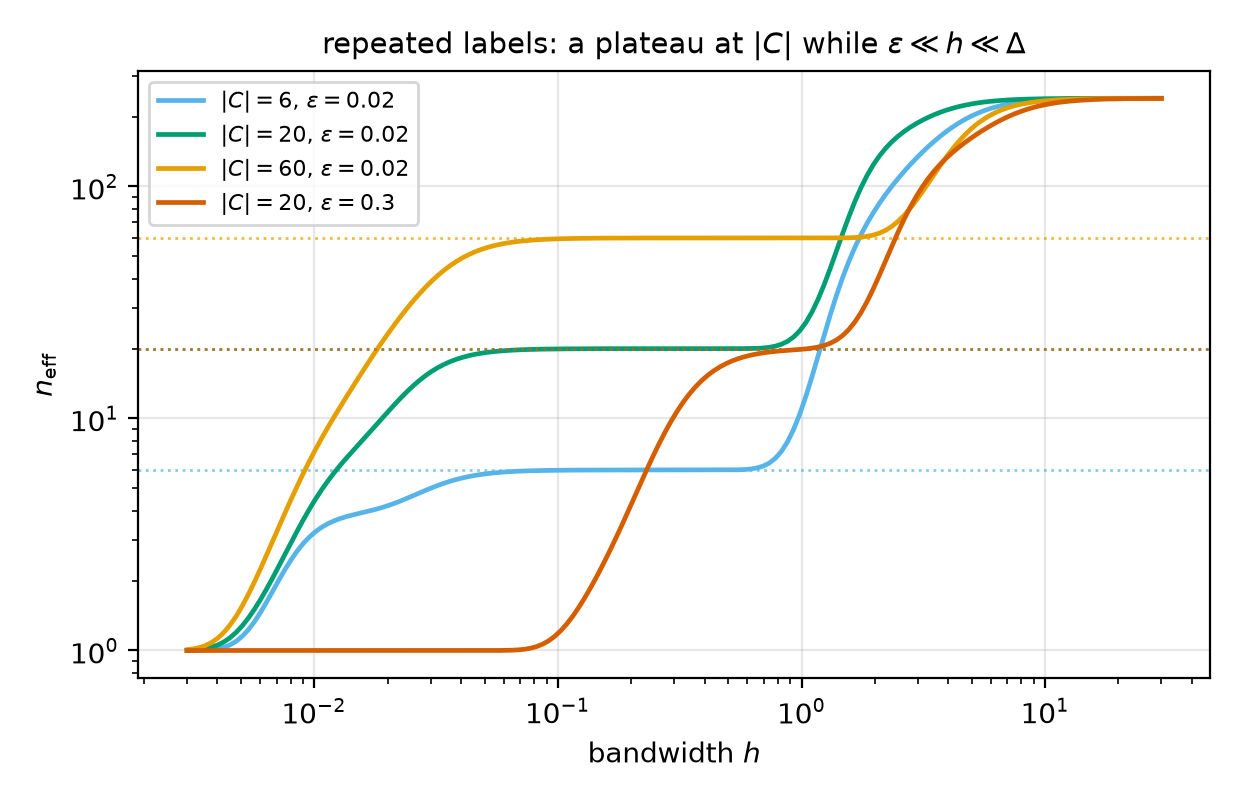
\includegraphics[width=0.72\textwidth]{fig_window.png}
\caption{The bandwidth window of Proposition~\ref{prop:nearduplicate}. With labels
in clusters of size $|C|$ at within-cluster scale $\varepsilon$ and between-cluster
scale $\Delta$, $n_{\mathrm{eff}}$ plateaus at $|C|$ exactly while
$\varepsilon\ll h\ll\Delta$: the model behaves as though conditioned on the cluster,
and the effective sample size counts the cluster rather than the dataset. The
lowest curve is the case that matters for the hypothesis---clusters loose relative
to their separation ($\varepsilon=0.3$)---where there is \emph{no} plateau at all
and $n_{\mathrm{eff}}$ runs from $1$ to $N$ with no usable $h$ in between.}
\label{fig:window}
\end{figure}

% ---- near-duplicate proposition ----
\begin{proposition}[Near-duplicate labels]
\label{prop:nearduplicate}
Fix a query $y$ and a subset $C\subseteq\{1,\dots,N\}$ with
$|y-y^i|\le\varepsilon$ for $i\in C$ and $|y-y^j|\ge\Delta$ for $j\notin C$, where
$\varepsilon<\Delta$. For the Gaussian kernel of bandwidth $h$, put
\[
\eta:=\frac{N-|C|}{|C|}\exp\!\Big(\!-\frac{\Delta^2-\varepsilon^2}{2h^2}\Big),
\qquad
\kappa:=\exp\!\Big(\frac{\varepsilon^2}{2h^2}\Big)\ \ge 1 .
\]
Then \emph{(a)} $\sum_{j\notin C}p_j^{(h)}(y)\le\eta$; \emph{(b)}
$p_i^{(h)}(y)/p_{i'}^{(h)}(y)\le\kappa$ for all $i,i'\in C$; and \emph{(c)}
$n_{\mathrm{eff}}(y)\ge|C|/(\kappa+|C|\eta^2)$.
Consequently, as $\varepsilon/h\to0$ and $\Delta/h\to\infty$ the index posterior
converges to the uniform law on $C$, the endpoint law to
$|C|^{-1}\sum_{i\in C}\delta_{x^i}$, and $n_{\mathrm{eff}}\to|C|$.
\end{proposition}

Figure~\ref{fig:window} plots the two bounds against $h$ and marks the usable window
they leave.

% ---- two-factor separation proposition ----
\begin{proposition}[The two mechanisms act on different factors]
\label{prop:factors}
In the factorisation \eqref{eq:kernel-field}, label smoothing modifies the label
factor $K_h(y-y^i)$ and therefore changes $p_1$ (Theorem~\ref{thm:endpoint});
interpolant noise rescales the spatial factor $\N(tx^i,s_t^2 I_d)$
\emph{isotropically and identically for every $i$}, leaving the endpoint law
unchanged (Proposition~\ref{prop:prop17}). The two remedies are therefore not
interchangeable.
\end{proposition}

% ---- finite-sample memorisation summary subsection ----
\subsection{Finite-sample memorisation (summary)}
\label{sec:d2summary}

Appendix~\ref{sec:theory-d2} adapts two representability results of the
unconditional gradient-variance literature \citep{gradvar2025} to the present
notation---a fixed finite \emph{unconditional} batch always admits an exact
zero-loss memorising field despite Proposition~\ref{prop:uncond}'s positive
population loss (Proposition~\ref{prop:memorize}), and resampling $x_0$ every
epoch is exactly what defeats that construction (Remark~\ref{rem:resample})---and
adds a new, problem-specific result: no finite-depth, finite-width network with
globally Lipschitz activations can equal the collapsed field's $1/(1-t)$ blow-up
\emph{pointwise} on all of $[0,1)$ (Remark~\ref{lem:norepr}). We state it as a
remark rather than a contribution because its reach is narrow: our sampler, like every
practical one, stops at $t=1-10^{-3}$, where $1/(1-t)$ is merely $10^3$ and a finite
network represents it comfortably. It rules out exact representation on the open
interval, not adequacy on the interval anyone integrates over. We keep that
pointwise claim separate from a loss floor: the only class for which we prove a
strictly positive floor is the Lipschitz-capped $\mathcal F_L$ of
Corollary~\ref{cor:floor}. The contrast with Proposition~\ref{prop:collapse} is
the point---conditional collapse needs no genericity argument and no fixed-batch
caveat, because $y^i$ pins down $i$ for every $x_0$, not merely with probability
one on a single draw.

\subsection{Scope: what is and is not predicted}

% ---- EXP-1 headline table ----
\begin{table}[htb]
\centering\small
\begin{tabular}{lccccc}
\toprule
& \multicolumn{5}{c}{iteration}\\
\cmidrule(l){2-6}
quantity & $10^2$ & $10^4$ & $10^5$ & $2\times10^5$ & $1\times10^6$ \\
\midrule
conditional $\tr\Cov$ & $1.08\pm0.02$ & $1.03\pm0.11$ & $0.58\pm0.18$ & $0.396\pm0.127$ & $0.120\pm0.054$\\
velocity rel.\ error vs.\ ($\star$) & $0.78\pm0.03$ & $0.75\pm0.07$ & $0.50\pm0.04$ & $0.40\pm0.05$ & $0.168\pm0.052$\\
$\|\text{mean}-x^i\|$ & $0.90\pm0.16$ & $0.87\pm0.20$ & $0.58\pm0.13$ & $0.38\pm0.10$ & $0.137\pm0.065$\\
$\|\text{mean}-\mu_{\mathrm{post}}\|$ & $0.15\pm0.06$ & $0.25\pm0.07$ & $0.52\pm0.10$ & $0.66\pm0.18$ & $0.816\pm0.172$\\
unconditional $\tr\Cov$ & $1.85\pm0.55$ & $1.93\pm0.16$ & $1.91\pm0.17$ & $1.926\pm0.171$ & ---\\
\bottomrule
\end{tabular}
\caption{EXP-1, mean$\pm$std over 5 seeds; the $10^6$ column is the cosine-schedule
run (no unconditional counterpart), whose between-seed spread makes it evidence of
\emph{stability} rather than a precise depth estimate. Same-seed reference values:
$\tr\Sigmapost=1.018\pm0.016$, $\tr\Xhat=1.931\pm0.162$---the unconditional row
matches the latter almost exactly, which is \eqref{eq:distinction} measured directly.}
\label{tab:exp1}
\end{table}

% ---- 5.4 problem-specification justification (C8) ----
This instance is deliberately chosen to be a genuine conditional inverse problem
rather than a classification-style one: the conditioning variable is the observed half
of the image, so it is continuous and high-dimensional ($k{=}1536$); many completions
are consistent with any given $y$, so a collapsed sampler is a real failure rather than
a near-optimal answer; and training runs long past the point of good calibration, with
checkpoints early and late. Those are the conditions under which posterior collapse is
worth measuring at all.

% ---- 5.4 atomicity, n_eff and seed paragraphs ----
\paragraph{The atomicity floor does not survive training.}
Proposition~\ref{prop:atomicity} proves that the smoothed population law is supported on
the training set for \emph{every} $h$. The trained network escapes it, progressively: the
fraction of generated samples lying on a training atom is $1.000$, $0.829$, $0.717$ and
$0.620$ at $h=0,4,5,6$, so at $h{=}6$ roughly $38\%$ of samples are off-atom. ``On an
atom'' is the nearest-neighbour criterion of \citet{yoon2023memorization} as used by
\citet{buchanan2025edge}, at their default: a sample counts as on-atom when its squared
distance to the nearest training image is at most $\tfrac19$ of its squared distance to
the second-nearest, i.e.\ a ratio of raw distances below $\tfrac13$. It is a relative
test and not floating-point equality, which for continuous image output would be
vacuous; the criterion is fixed across all four bandwidths, so the trend is a trend in
the data and not in the threshold
(\texttt{src/metrics/memorization.py}). The value
of exactly $1.000$ at $h{=}0$ rules out ODE discretisation as the explanation, since the
same integrator is used throughout. Atomicity is thus a property of the population
minimiser that finite capacity partially undoes---which is good news for sample quality
and bad news for treating Proposition~\ref{prop:atomicity} as a statement about trained
models. It is also the one place in this paper where a proved property of the exact
minimiser is measurably \emph{not inherited} by the network that approximates it. We
avoid saying the proposition is violated: it is a statement about the population
minimiser, and a finite trained model is not that object, so what the measurement shows
is $P_\theta\ne P_h^\star$ and not that Proposition~\ref{prop:atomicity} fails.

% ---- Limitations: atomicity paragraph, trimmed ----
\paragraph{A proved property of the population minimiser that the trained model
does not inherit.} Proposition~\ref{prop:atomicity} shows the smoothed law is supported on the
training set for every $h$, and Section~\ref{sec:cifarddpm} measures the fraction of
generated samples actually on an atom as $1.000$, $0.829$, $0.717$, $0.620$ at
$h=0,4,5,6$. The obstruction is therefore exact for the object the theory describes and
only approximate for the object practitioners train, with the gap widening as $h$ grows.
We do not have a quantitative account of that gap, and it is the clearest instance in
this paper of the population/finite-network distinction biting: everywhere else the two
agree in direction, here they disagree about a set-valued statement that is either true
or false.

% ---- Limitations: remedies paragraph, trimmed ----
\paragraph{We do not benchmark against the remedies practitioners already use.} Early
stopping, weight averaging, condition dropout, caption randomisation and
classifier-free guidance scale are all deployed against exactly the symptom studied
here, and we compare against none of them. Our claim is therefore diagnostic, not
prescriptive: $\Covh$ is a reference a trained model can be audited against, and label
smoothing is what that reference describes---but which intervention one should actually
reach for, and at what cost to sample quality, is not settled by anything in this paper.
Caption randomisation is the one case where our analysis makes a concrete prediction
(it is label smoothing, so Theorem~\ref{thm:endpoint} applies to it and the atomicity
ceiling binds it), and testing that prediction against the practice is the obvious next
experiment.

% ---- moved from the introduction: what each factor is good for ----
\paragraph{The two factors are not one result applied to opposite halves of a product.}
The sharpest way to see this is to ask what each factor of \eqref{eq:kernel-field} can
be used for. The spatial factor is imposed by the clock: its bandwidth is $1-t$, it is
common to the conditional and unconditional fields alike, and it cannot be tuned, swept,
or removed. The label factor is a modelling choice, and everything this paper extracts
follows from that: an $h$-indexed family with a parameter-free reference curve to audit
against (Proposition~\ref{prop:moments}), the two limits $h\to0$ and $h\to\infty$
(Corollaries~\ref{cor:zerobw} and~\ref{cor:infbw}), a bandwidth window set by the
geometry of the labels (Proposition~\ref{prop:nearduplicate}), and an $h$-independent
obstruction, which is a statement about the whole family and so needs a family to state
(Proposition~\ref{prop:atomicity}). Classifier-free guidance is the cleanest case: the
conditional and unconditional fields differ in exactly one place---the label factor,
since the spatial factor is identical in both---so guidance is \emph{entirely} a
label-factor phenomenon, and Propositions~\ref{prop:cfg} and~\ref{prop:cfgatom} are not
available from a reading of the other factor at all. Figure~\ref{fig:factorisation} shows
the two factors separately, and their product, on the real $d{=}2$ instance.

\begin{figure}[htb]
\centering
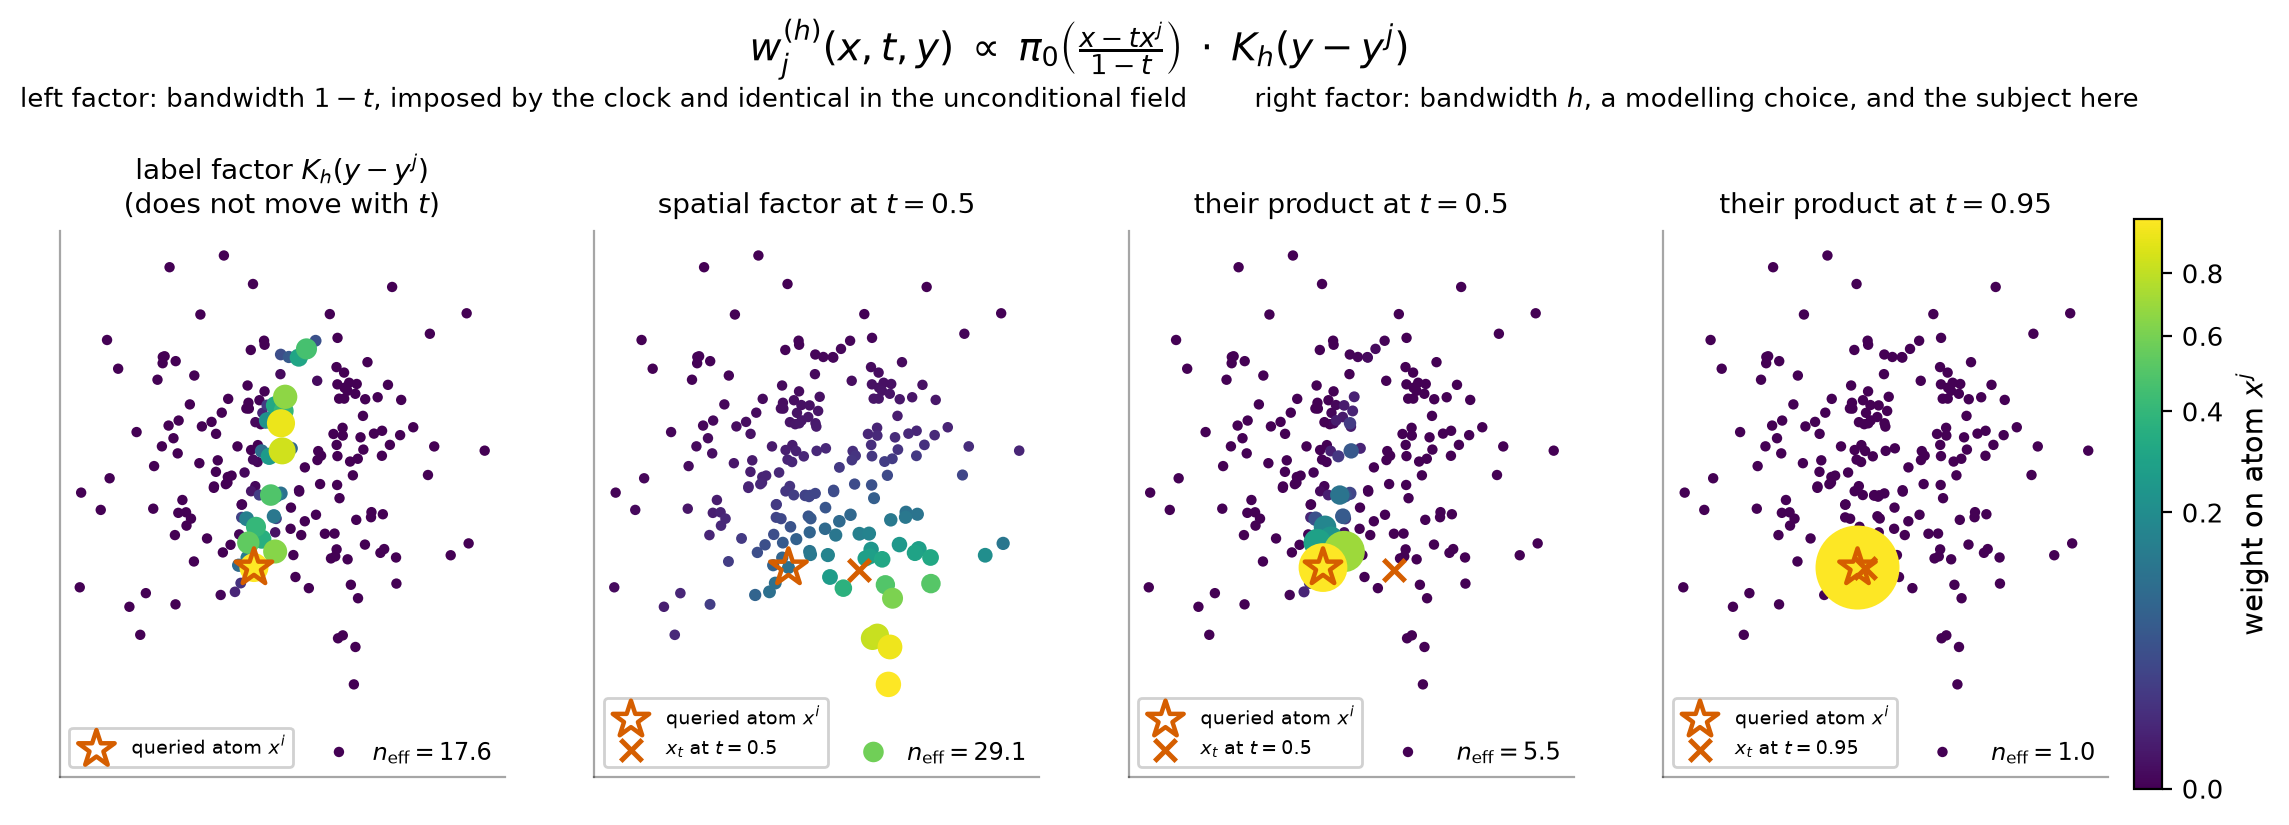
\includegraphics[width=0.98\textwidth]{fig_factorisation.png}
\caption{The index posterior, factor by factor, on the real $d{=}2$ instance
($N{=}200$, $h{=}0.1$), with atoms coloured and sized by their weight. The
\emph{label} factor selects a band of eligible atoms and does not move with $t$
($n_{\mathrm{eff}}=17.6$). The \emph{spatial} factor at mid-time selects a different,
broader region ($29.1$). Neither alone picks out an atom; their product---the weight
the flow actually follows---is supported on the intersection ($5.5$), and by $t=0.95$
it has collapsed onto one ($1.00$). The two bandwidths are not on the same footing:
$1-t$ is imposed by the clock and is identical in the unconditional field, whereas
$h$ is a modelling choice. Everything this paper extracts comes from the right-hand
factor, which is what separates it from a reading of the left one
\citep{smola2026support}.}
\label{fig:factorisation}
\end{figure}

% ---- related-work comparison table ----
\begin{table}[htb]
\centering\small
\renewcommand{\arraystretch}{1.15}
\begin{tabular}{@{}p{0.20\textwidth}p{0.15\textwidth}p{0.28\textwidth}p{0.30\textwidth}@{}}
\toprule
work & conditioning & what it establishes & what it leaves open, and we supply\\
\midrule
\citet{scarvelis2025closedform} & unconditional & closed-form empirical denoiser is a
kernel-weighted average of training points, degenerating to a mixture of atoms &
the \emph{conditional} case, where the label identifies one atom rather than
reweighting all of them\\
\citet{chen2026scoresmoothing} & unconditional & smoothing the empirical score as the
escape from memorisation & smoothing the \emph{label}, and the exact endpoint law it
induces\\
\citet{smola2026support} & conditional & the \emph{spatial} factor
$\pi_0(\tfrac{x-tx^i}{1-t})$ is a Nadaraya--Watson smoother with bandwidth the flow
time $1-t$, sharpening to nearest-neighbour as $t\to1$ & the \emph{label} factor
$K_h(y-y^i)$ of the same product \eqref{eq:kernel-field}, whose bandwidth is a
modelling choice; and the endpoint law and its moments rather than the field. The two
readings compose; neither implies the other\\
\citet{gu2023memorization} & conditional & unique/random labels sharply increase
memorisation at CIFAR and FFHQ scale, empirically & \emph{why}: informativeness is
irrelevant, identification is everything
(Proposition~\ref{prop:collapse}), which our shuffled-label experiment tests directly\\
\citet{somepalli2023copying} & text & replication is common with text conditioning and
rare without it; randomising captions mitigates & that this asymmetry \emph{is}
Eq.~\eqref{eq:distinction}, and that caption randomisation is label smoothing in the
sense of Theorem~\ref{thm:endpoint}\\
\citet{ho2022cascaded}; \citet{sadat2024cads} & conditional & conditioning noise as
practice; annealed at inference to restore conditional diversity & that the restored
variance is an exact Nadaraya--Watson mixture over training atoms---hence a
parameter-free reference, and a false certificate for posterior recovery\\
\citet{buchanan2025edge} & unconditional & memorisation/generalisation phase transition
as denoiser capacity $M$ ranges over $K\to N$ & the label/bandwidth analogue
$h\colon0\to\infty$ (Corollaries~\ref{cor:zerobw},~\ref{cor:infbw}); neither result
subsumes the other\\
\bottomrule
\end{tabular}
\caption{Where this paper sits. The rows above the rule on conditioning noise own the
memorisation side; the two below own the remedy side. What no row supplies is the object
connecting them---that the remedy is exactly kernel regression over the atoms the
memorisation produces, with the ceiling that entails.}
\label{tab:related}
\end{table}

% ---- regularity conventions (B7) ----
\paragraph{Three conventions, stated rather than assumed.} \emph{(i) Versions.} The
minimiser of an $L^2$ projection is unique only up to a null set
(Proposition~\ref{prop:projection}), yet the results below assert formulas ``for every
$x$ and $t<1$''. What we exhibit in each case is a distinguished \emph{continuous}
version: the weights in \eqref{eq:kernel-field} are ratios of everywhere-positive
smooth functions (Lemma~\ref{lem:cov}), so the formula defines a continuous field on
$\R^d\times[0,1)$, and every pointwise claim is a claim about that version. Any other
minimiser agrees with it a.e., which is all the flow sees. \emph{(ii) Endpoints.}
$p_1$ always denotes the weak limit $\lim_{t\uparrow1}p_t$, never a value attained at
$t=1$; the field is undefined there. We establish that the limit exists wherever we use
it, each time from almost-sure convergence of the interpolant rather than by appeal to a
general theorem, and Lemma~\ref{lem:wellposed} is deliberately narrowed so as not to
claim existence in general. \emph{(iii) Where the flow is well posed.} The $1/(1-t)$
factor means no statement here extends to the closed interval. All flows are solved on
$[0,1)$, where Lemma~\ref{lem:wellposed} gives existence, uniqueness and a growth bound;
the blow-up at $t=1$ is the mechanism under study, not a technical nuisance to be
regularised away.

% ---- atomicity floor scaling (B5) ----
\paragraph{How large is the floor, and where does it bind?}
Proposition~\ref{prop:atomicity} gives an $h$-independent floor but not its size, and
the paper measures it small (Appendix~\ref{sec:aux}), which invites the objection that
the obstruction is a curiosity. The scaling answers that, and it needs one distinction the earlier version of this
paragraph elided. Zador's theorem \citep[Ch.~6]{graf2000quantization} says the
\emph{optimal} $N$-point approximation of a measure with a non-degenerate absolutely
continuous part on $\R^d$ has $W_2$ error decaying as $N^{-1/d}$. Our floor is over the
$N$ atoms the training set happened to draw, which are i.i.d.\ and not placed
optimally, so Zador bounds it from \emph{below}---the training atoms are one admissible
$N$-point set---which is the direction the argument needs. Whether i.i.d.\ atoms attain
the same rate is a separate question about a random design, and we answer it with a
measurement rather than a citation---evidence at the dimensions we tested, not a
theorem for all $d$ (\texttt{scripts/verify\_atom\_floor\_scaling.py}, standard
Gaussian target, atoms i.i.d.\ from the same law). At $d=3,5,8$ the exponent is
attained: fitting $\log F_N$ on $\log N$ over $N\in[200,3200]$ gives slopes $-0.612$,
$-0.379$ and $-0.249$ against the predicted $-2/d=-0.667$, $-0.400$, $-0.250$. At
$d{=}2$ it is \emph{not}: the fitted slope is $-0.846$, and the reason is a
logarithmic correction that the optimal quantiser does not pay---$F_N\,N/\log N$ is flat to within $1.05\times$ across that
range while $F_N\,N$ drifts by $1.52\times$, so the i.i.d.\ floor there is
$\Theta(\log N/N)$, not $\Theta(1/N)$. The gap is real but works against the sceptic:
random atoms are \emph{worse} than optimal ones, so the obstruction is if anything
larger than the quantisation rate suggests. In any case the exponent is the whole
story:
\[
N^{-1/d}=0.071 \ \text{ at our default } (d,N)=(2,200),
\quad
N^{-1/d}=0.9975 \ \text{ at } (3072,2000).
\]
At $d{=}2$ two hundred atoms densely approximate the posterior, which is why we measure
the floor and find it negligible; at image dimension the same number of atoms reduces
the approximation error by a quarter of one percent. The atomicity obstruction is
therefore not merely present but \emph{dominant} in exactly the regime where diversity
is wanted, and negligible in the regime where it is easy to measure. We report both,
and take this to be the reason the obstruction deserves the weight we give it.

% ---- guidance commentary ----
\begin{proposition}[Guidance lands on a training atom]
\label{prop:cfgatom}
Assume $x^1,\dots,x^N$ are distinct, let $w\ge0$, and let $x_t$ solve
$\dot x_t=v_w(x_t,t)$ on $[0,1)$ with $x_t\to x^*$ as $t\uparrow1$. Assume the nearest
atom to $x^*$ is unique, and write $i^*=\arg\min_j|x^*-x^j|$. Then
\begin{enumerate}[label=(\alph*),leftmargin=2em]
\item if $h>0$, $x^*=x^{i^*}$: the limit is a training atom; and
\item if $h=0$ with distinct labels, $x^*=x^i$ for every $w\ge0$: the limit is the
  \emph{conditioned} atom, so guidance is entirely inert under hard conditioning.
\end{enumerate}
\end{proposition}

So guidance can change \emph{which} atom is reached once the label is smoothed---the
choice of $i^*$ depends on the trajectory, hence on $w$---but never reaches anything
else, and under hard conditioning it cannot even do that.
Figure~\ref{fig:guidance} integrates the exact guided field and shows both halves.

\begin{figure}[htb]
\centering
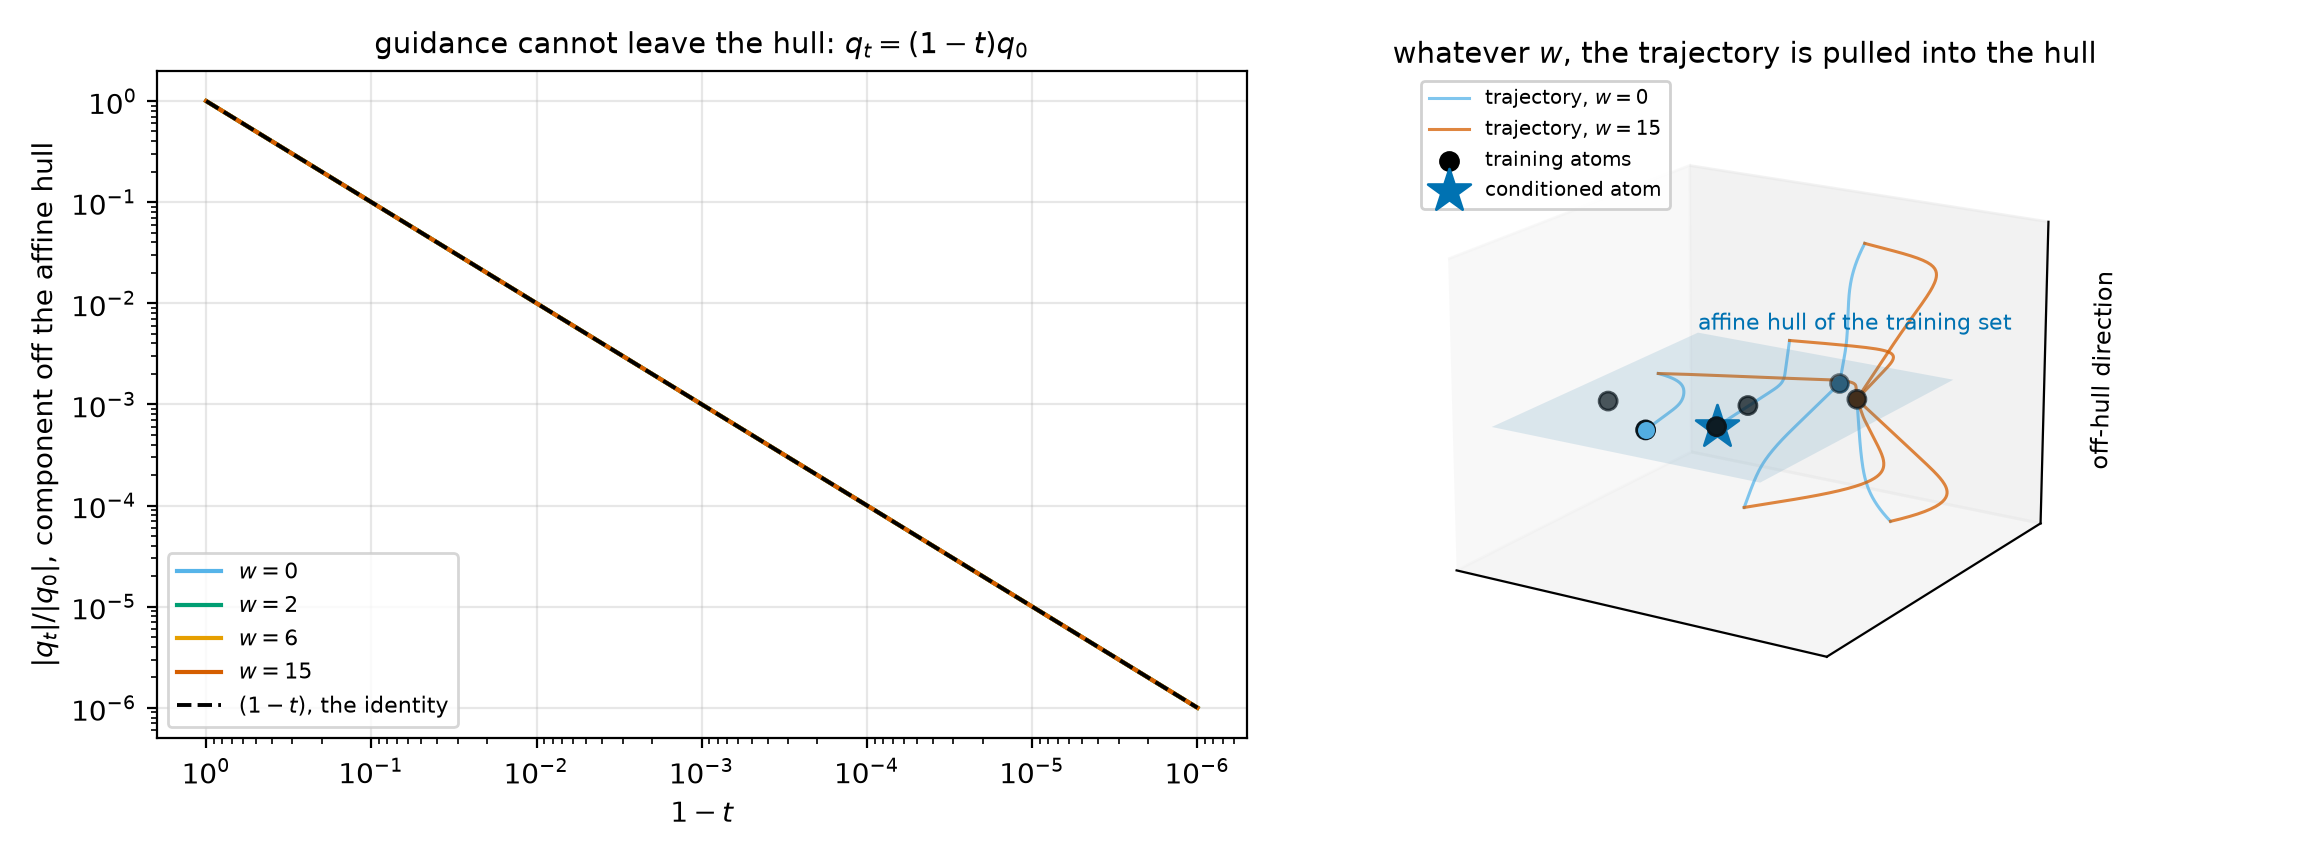
\includegraphics[width=0.94\textwidth]{fig_guidance.png}
\caption{Proposition~\ref{prop:cfg}, drawn. \textbf{Left}: the component of the
guided trajectory orthogonal to the affine hull of the training set, normalised by
its initial value. For every guidance weight it lies exactly on $(1-t)$ over six
decades---the identity $q_t=(1-t)q_0$ the proof turns on, which holds because the
guided target is an affine combination of atoms and so is annihilated by the
orthogonal projection. \textbf{Right}, in three dimensions because the result is
about dimension: six atoms spanning a plane in $\R^3$, and trajectories started
deliberately off that plane. Whatever $w$, they are pulled into it. When $N\le d$
the hull is Lebesgue-null, so no guidance weight yields an absolutely continuous
conditional law.}
\label{fig:guidance}
\end{figure}

Two things are worth separating here. What Proposition~\ref{prop:cfg} proves is a
statement about \emph{dimension}: guidance moves mass around inside a set of dimension
at most $N-1$ and cannot leave it. In the image regime that is already decisive
---$N{=}2000$ atoms in $d{=}3072$ leaves a null set---but at $N>d$ the affine hull is
all of $\R^d$ and the proposition says nothing. What we \emph{observe}, integrating the
exact guided field, is stronger: endpoints land on the atoms themselves, to integrator
accuracy, at every $w$ we tried, and increasing $w$ changes \emph{which} atom is
reached rather than whether an atom is reached
(\texttt{scripts/verify\_cfg\_affine.py}; the identity \eqref{eq:cfgorth} is
reproduced to six decimal places for $h\in\{0,0.7\}$ and $w\in\{0,3,12\}$). Proposition~\ref{prop:cfgatom} proves it, assuming only that the trajectory
converges at all.

% ---- near-duplicate commentary ----
This is the regime that occurs in practice---captions or labels that are close but
not identical---and it makes the bandwidth window explicit. Both conditions can hold
at once exactly when $\varepsilon\ll h\ll\Delta$, so a usable $h$ exists precisely when
clusters are tight relative to their separation; inside that window the model behaves as
though conditioned on the cluster, with $n_{\mathrm{eff}}$ counting the cluster and not
the dataset. Note what does \emph{not} improve: the endpoint law is still a finite sum
of point masses, now $|C|$ of them, so Proposition~\ref{prop:atomicity} applies
unchanged. Near-duplicate labels buy effective sample size, not continuity.

% ---- bandwidth-expansion caveats (B8) ----
Both restrictions matter for what follows: a pointwise, homoscedastic expansion should
\emph{not} be expected to describe an image model, where $\Sigma(\cdot)$ certainly
varies with the conditioning image and most evaluation conditions sit near the boundary
of a $1536$-dimensional label support. The across-condition slope of $0.481$ measured
in Section~\ref{sec:cifarddpm} is what that failure to transfer looks like, and we read
it that way rather than as a refutation of \eqref{eq:expansion} at the point where it
is claimed.

% ---- Lipschitz representation floor (B4 / former contribution 5) ----
\subsection{Finite capacity: a genuine representation floor}
\label{sec:theory-floor}

The results so far describe the population minimiser over \emph{all}
square-integrable fields; a trained network is restricted to a finite-capacity
class. Here is one concrete way that restriction alone forces a positive loss floor,
independent of any optimisation difficulty.

\begin{proposition}[Lipschitz lower bound]
\label{prop:liplb}
Fix $i$, $t<1$, $f_i(x,t)=(x^i-x)/(1-t)$, and suppose $v(\cdot,t,y^i)$ is
$L$-Lipschitz in $x$. Under $X_t\mid I=i\sim\N(tx^i,(1-t)^2 I_d)$,
$\E[|v(X_t,t,y^i)-f_i(X_t,t)|^2\mid I=i]\ge d\,[1-L(1-t)]_+^2$.
\end{proposition}

\begin{corollary}[Loss floor under a uniform Lipschitz constraint]
\label{cor:floor}
For $\mathcal F_L=\{v:\operatorname{Lip}_x v(\cdot,t,y^i)\le L\ \forall t,i\}$ with
$L\ge1$ and $t\sim\mathrm{Unif}(0,1)$,
\begin{equation}
\inf_{v\in\mathcal F_L}L_0(v)\ \ge\ d\int_{1-1/L}^1[1-L(1-t)]^2\,dt\ =\ \frac{d}{3L}\ >\ 0.
\label{eq:floor}
\end{equation}
More generally, if the Lipschitz constant is allowed to depend on time,
$\operatorname{Lip}_xv(\cdot,t,y^i)\le L(t)$, the same pointwise bound integrates to
\begin{equation}
\inf_{v\in\mathcal F_{L(\cdot)}}L_0(v)\ \ge\ d\int_0^1\big[1-L(t)(1-t)\big]_+^2\,dt .
\label{eq:floorlt}
\end{equation}
\end{corollary}

\eqref{eq:floorlt} is the honest form of the statement, and it changes how
\eqref{eq:floor} should be read. The uniform-$L$ floor is an artefact of the
uniformity: the integrand in \eqref{eq:floorlt} vanishes identically as soon as
$L(t)\ge1/(1-t)$ for a.e.\ $t$, so a network whose Lipschitz constant in $x$ grows like
$1/(1-t)$ near the endpoint---which a time-conditioned network is free to do, and which
the target field itself does---faces no floor at all from this mechanism. That is
consistent with what we measure: Appendix~\ref{sec:aux} finds the $d/(3L)$ value some
$50\times$ below the observed plateau. We therefore do not offer this as an explanation
of the plateau, and say so in Section~\ref{sec:limitations}; we retain it because ruling
a mechanism out is worth recording, and because \eqref{eq:floorlt} localises what would
have to be measured---the profile $L(t)$ near $t=1$, not a single constant---for the
question to be settled.

Two warnings temper \eqref{eq:floor}. First, the bound is \emph{conditional} on the
constraint: an MLP with unbounded weights lies in no fixed $\mathcal F_L$, and by
universal approximation $\inf_\theta L(v_\theta)$ may be $0$; what we prove is that
any architecture with $\operatorname{Lip}_x v_\theta\le L$ cannot beat $d/(3L)$.
Second, it does not bind in our experiments: with $d=2$ and a trained
$\operatorname{Lip}_x$ of order $10^1$--$10^2$, the floor is of order $10^{-2}$,
one to two orders of magnitude below the loss plateau $0.48$ observed at $2\times10^5$ iterations (it falls to $0.36$ by $7\times10^5$, so the gap is if anything understated).
Corollary~\ref{cor:floor} is therefore best used as a \emph{measurement}---estimate
$L$, compare $d/(3L)$ to the plateau, report which gap dominates
(Appendix~\ref{sec:aux})---and that measurement rules the representation
explanation \emph{out} here.

\subsection{Where the standard remedies stand}
\label{app:remedies}

Five interventions are deployed
against this symptom in practice, and the account here settles four without new
experiments. \emph{Guidance} cannot leave the training set's affine hull at any weight
and lands on an atom---under hard conditioning the conditioned atom itself, so there it
is fully inert. \emph{Caption randomisation} is label smoothing, so
Theorem~\ref{thm:endpoint} describes it exactly and the atomicity ceiling binds it.
\emph{Condition dropout} leaves the minimiser of Proposition~\ref{prop:projection}
unchanged conditionally on a real label, so it too does not move the conditional
endpoint; what it supplies is the unconditional field guidance then combines.
\emph{Early stopping} we measure: at $h{=}6$ the aggregate ratio passes through $0.98$ at
$8000$ iterations and drifts to $1.18$ by $60000$, while at $h{=}4$ it never arrives
within the budget (Appendix~\ref{app:deferred}). \emph{Weight averaging} we have not
analysed. What we do not offer is a comparison at matched sample quality, the axis a
practitioner actually trades against.

Figure~\ref{fig:interventions} draws the four settled interventions as flows rather
than as statements: each panel integrates the exact population field of that
intervention from the same $160$ draws of $x_0$, on the instance of
Figure~\ref{fig:mechanism}, so the taxonomy---inert, atom-preserving, reweighting,
support-moving---can be read off the endpoints.

\begin{figure}[htb]
\centering
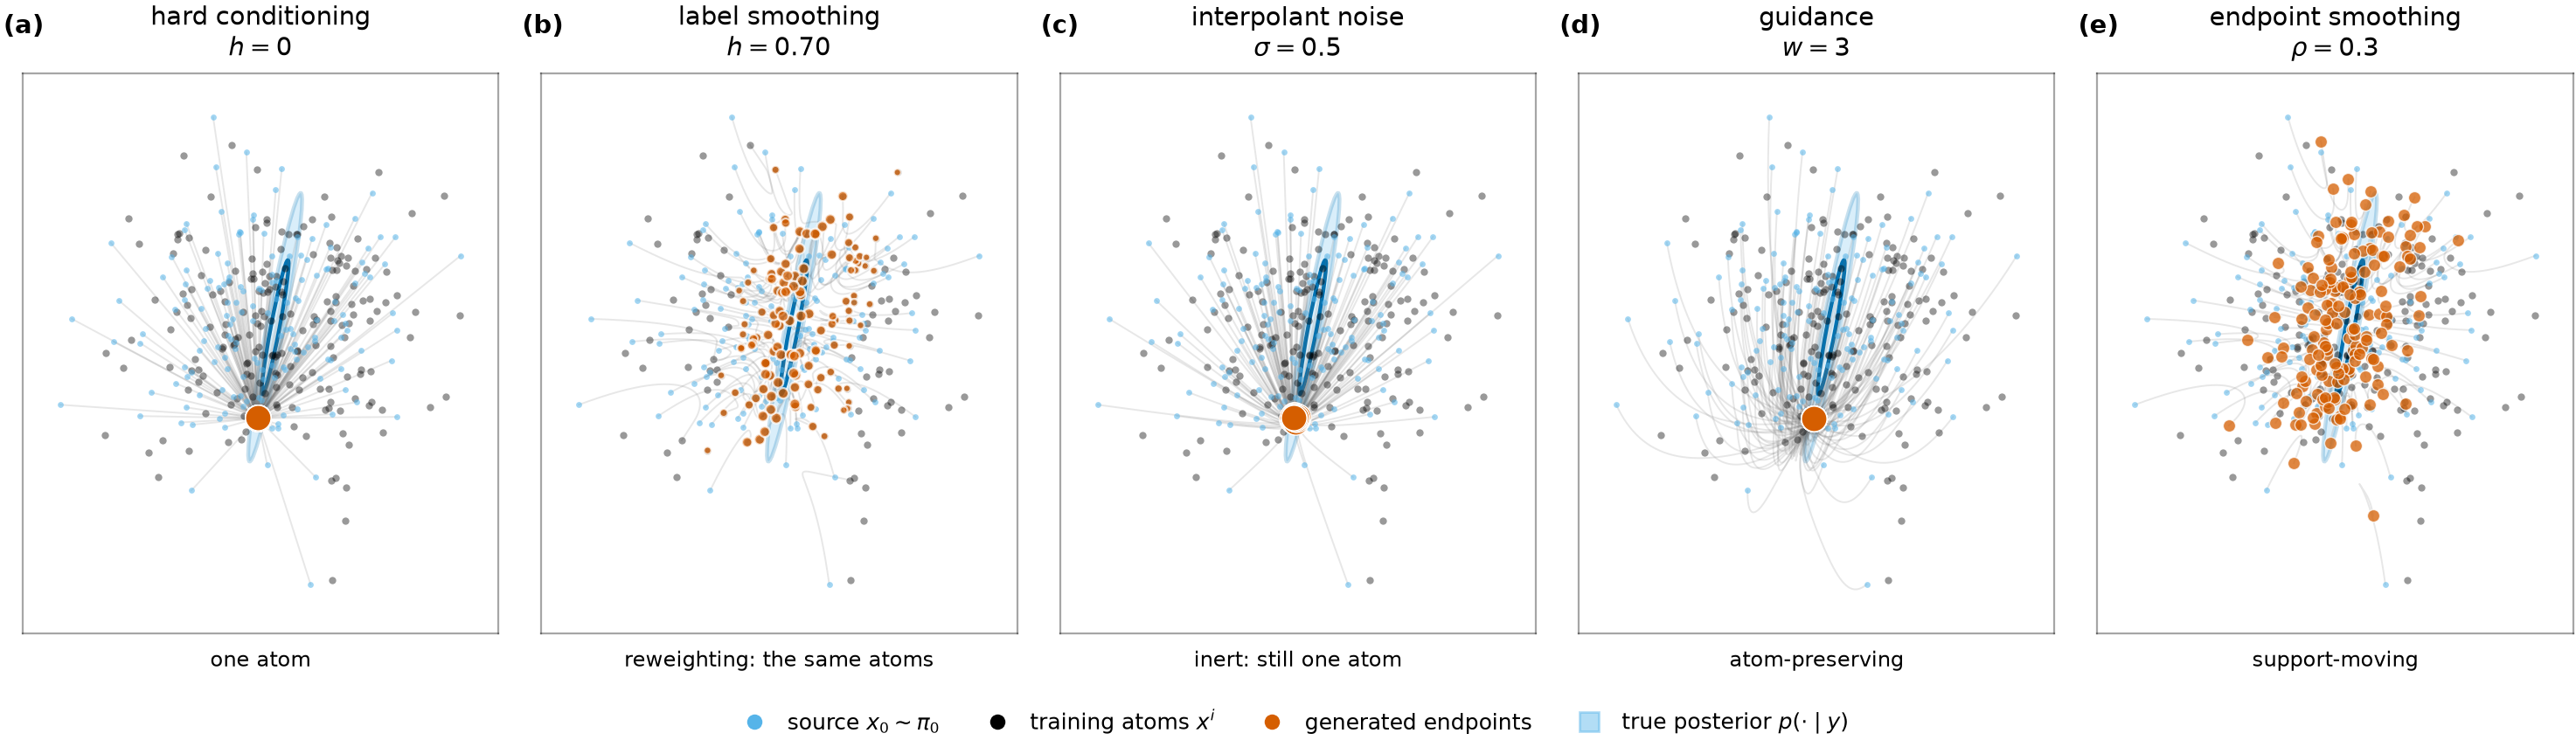
\includegraphics[width=\textwidth]{fig_interventions.png}
\caption{The four interventions, as exact population flows on one condition of the
EXP-1 instance. (a) hard conditioning: every path lands on the labelled atom. (b) label
smoothing at $h^\star$: the same atoms, reweighted by $p^{(h)}_i$ (marker area), which
is Theorem~\ref{thm:endpoint}. (c) interpolant noise at $\sigma{=}0.5$: the paths are
different and the endpoint is not---$\gamma(1)=0$, so the endpoint law is the same point
mass at every noise level (Proposition~\ref{prop:prop17}). (d) guidance at $w{=}3$:
atom-preserving, and under hard conditioning it is the conditioned atom itself
(Proposition~\ref{prop:cfg}). (e) endpoint smoothing at $\rho{=}0.30$: the only one of
the four whose support leaves the atoms (Proposition~\ref{prop:tgtnoise}). Produced by
\texttt{scripts/make\_flow\_portraits.py}, which checks its own field against
\eqref{eq:kernel-field} before drawing.}
\label{fig:interventions}
\end{figure}

\subsection{Error survival and the loss form: statements and discussion}
\label{app:survivaltheory}

Section~\ref{sec:survival} states what follows in summary. The results of
Section~\ref{sec:theory} describe the population minimiser and none says what happens to
a model merely \emph{close} to it; the proposition below closes that gap, and the answer
is a contraction estimate rather than the growth estimate one might expect.

\begin{proposition}[Error survival]
\label{prop:survival}
Fix $i$, let $h=0$ with distinct labels, and let $v$ be any locally Lipschitz field.
Write $\Delta(x,t):=v(x,t,y^i)-\vstarz(x,t,y^i)$ for its error against the exact
collapsed field, let $x^v_t$ solve $\dot x_t=v(x_t,t,y^i)$ from $x_0$, and let
$x^\star_t=(1-t)x_0+tx^i$ be the exact trajectory from the same $x_0$. Then for
$t<1$, with $e_t:=x^v_t-x^\star_t$, the \emph{identity}
\begin{equation}
e_t\;=\;(1-t)\int_0^t\frac{\Delta(x^v_s,s)}{1-s}\,ds
\label{eq:survival-id}
\end{equation}
holds, and in particular
\begin{equation}
|e_t|\;\le\;(1-t)\int_0^t\frac{|\Delta(x^v_s,s)|}{1-s}\,ds .
\label{eq:survival}
\end{equation}
Consequently:
\begin{enumerate}[label=(\alph*),leftmargin=2em]
\item \emph{(bounded errors do not survive)} if
  $\int_0^t|\Delta(x^v_s,s)|^2ds\le\varepsilon^2$ then
  $|e_t|\le\varepsilon\sqrt{(1-t)t}\le\varepsilon\sqrt{1-t}$, so a sampler stopping
  at $t=1-\delta$ has $|e_{1-\delta}|\le\varepsilon\sqrt\delta$, which vanishes with
  $\delta$ \emph{for every} finite $\varepsilon$;
\item \emph{(what the bound gives)} if $|\Delta(x,t)|\le c\,(1-t)^{-a}$ with $a>0$
  then $|e_t|\le\frac{c}{a}\big((1-t)^{1-a}-(1-t)\big)$, which at $a=1$ reads
  $|e_t|\le c\,t\le c$. Hence $\lim_{t\uparrow1}|e_t|=0$ when $a<1$, and
  $\limsup_{t\uparrow1}|e_t|\le c$ when $a=1$. For $a>1$ the right-hand side diverges
  and \eqref{eq:survival} constrains $e_t$ not at all---a diverging upper bound is
  not a diverging quantity, and $e\equiv0$ satisfies it. That case is settled by
  (c), not by (b);
\item \emph{(the bound is attained, so the threshold is real)} fix a unit vector $u$
  and take the spatially constant error $\Delta(x,t)=c\,(1-t)^{-a}u$, for which
  $v=\vstarz+\Delta$ is locally Lipschitz with $\Delta$ having Lipschitz constant
  $L_\Delta=0$ in $x$. Then \eqref{eq:survival-id} evaluates in closed form:
  \begin{equation}
  e_t=\frac{c}{a}\big((1-t)^{1-a}-(1-t)\big)\,u\quad(a>0),
  \qquad e_t=-c\,(1-t)\log(1-t)\,u\quad(a=0),
  \label{eq:survival-sharp}
  \end{equation}
  so \eqref{eq:survival} holds with equality for every $t<1$. Therefore
  $\lim_{t\uparrow1}|e_t|$ is $0$ for $a<1$, is exactly $c$ for $a=1$, and is $+\infty$
  for $a>1$: the trichotomy is realised and not merely permitted;
\item \emph{(what a surviving deviation requires)} write
  $I(t):=\int_0^t\Delta(x^v_s,s)(1-s)^{-1}ds$ for the accumulated weighted error, so
  that \eqref{eq:survival-id} reads $e_t=(1-t)I(t)$. Then for any $\Delta$ and any
  $e_\star\in\R^d$,
  \begin{equation}
  \lim_{t\uparrow1}e_t=e_\star
  \iff
  I(t)=\frac{e_\star}{1-t}+o\big((1-t)^{-1}\big) .
  \label{eq:survival-conv}
  \end{equation}
  Since $e_t=(1-t)I(t)$ identically, the behaviour of $e_t$ at the endpoint is exactly
  the behaviour of $I$ at the scale $(1-t)^{-1}$, and the cases are exhaustive: if
  $|I(t)|=o((1-t)^{-1})$ then $e_t\to0$; if $(1-t)I(t)$ converges to some
  $e_\star\ne0$---equivalently, if $I$ sits at that scale \emph{with a limiting
  direction}---then $e_t\to e_\star$; if $(1-t)|I(t)|\to\infty$ then $|e_t|\to\infty$
  and there is no endpoint; and if $(1-t)I(t)$ stays bounded without converging, $e_t$
  has no limit either. In particular a nonzero endpoint deviation \emph{requires} the
  accumulated weighted error to attain exactly the $(1-t)^{-1}$ scale, and to do so in a
  direction that does not cancel: growing more slowly than that scale is annihilated
  by the factor $(1-t)$, whatever the pointwise behaviour of $\Delta$ that produced it.
\end{enumerate}
\end{proposition}

The reading is that the collapsed field is \emph{self-enforcing}. Its linear part is
$-\tfrac{1}{1-t}I_d$, a contraction whose strength diverges as $t\to1$, and that
contraction annihilates any perturbation that does not itself diverge at rate
$1/(1-t)$. A model can therefore retain conditional variance only by carrying an
endpoint-scale $1/(1-t)$ accumulated error---by failing, in the accumulated sense
part~(d) makes precise, to reproduce the blow-up---and the deviation it keeps is, to
leading order, the coefficient of that failure. This closes a loop the paper already
had open: Remark~\ref{lem:norepr} observes that no finite network with globally
Lipschitz activations represents $1/(1-t)$ pointwise on $[0,1)$, and
\eqref{eq:survival-conv} states the converse as an exact asymptotic rather than as a
word. We are deliberate about its form. It constrains
$I(t)=\int_0^t\Delta(x_s^v,s)(1-s)^{-1}ds$, not $\Delta$ pointwise: an error can
oscillate, or be large only on a thin set of times, and what survives depends on the
accumulation alone---the fourth case of~(d) is realised by an error of critical
magnitude whose direction turns forever and never settles
(Appendix~\ref{app:survival}). What the proposition does \emph{not} give is a pointwise
converse of the form ``$e_1\ne0\Rightarrow\Delta=\Theta((1-t)^{-1})$'', and we do not
claim one. Read this way the observed plateau is the size of the weighted integral the
network's error accumulates rather than an unexplained residual, and the collapse we
measure over training (Table~\ref{tab:exp1}, Section~\ref{sec:cifarddpm}) is that
quantity shrinking.

The bound as stated is pathwise, integrating along the model's own trajectory, which is
not a quantity anyone measures. It converts into the training loss with one extra
hypothesis, weaker than it first looks.

\begin{assumption}[Lipschitz error]
\label{as:lipschitz}
In the setting of Proposition~\ref{prop:survival}, the error
$\Delta(\cdot,t)=v(\cdot,t,y^i)-\vstarz(\cdot,t,y^i)$ is $L_\Delta$-Lipschitz in $x$ for
a.e.\ $t\le T$.
\end{assumption}

\begin{corollary}[Loss form]
\label{cor:lossform}
In the setting of Proposition~\ref{prop:survival} and under
Assumption~\ref{as:lipschitz}, let
\[
\mathcal L_i(v)\;:=\;\E_{t\sim\mathrm{Unif}(0,1)}\,\E_{X_0\sim\pi_0}
\big|v(X_t,t,y^i)-U\big|^2,\qquad X_t=(1-t)X_0+tx^i,\ U=x^i-X_0,
\]
be the flow-matching loss at index $i$, and write
$\mathcal E(t):=\big(\E_{X_0}|x^v_t-x^\star_t|^2\big)^{1/2}$ for the root-mean-square
deviation over initial conditions. Then for $t\le T$,
\begin{equation}
\mathcal E(t)\;\le\;e^{L_\Delta t}\,\sqrt{\mathcal L_i(v)}\;\sqrt{t(1-t)},
\qquad\text{so}\qquad
\mathcal E(1-\delta)\;\le\;e^{L_\Delta}\sqrt{\mathcal L_i(v)\,\delta}.
\label{eq:lossform}
\end{equation}
Consequently the conditional second moment about the memorised atom obeys
$\big(\E|x^v_{1-\delta}-x^i|^2\big)^{1/2}\le e^{L_\Delta}\sqrt{\mathcal L_i(v)\delta}
+\delta\,\big(\E|X_0-x^i|^2\big)^{1/2}$.
\end{corollary}

Note which Lipschitz constant is assumed: that of the \emph{error} $\Delta$, not of the
field, whose constant $1/(1-t)$ diverges by construction. The distinction is what keeps
the hypothesis from excluding the phenomenon---an error $c\,(1-t)^{-1}u$, the kind
part~(b) identifies as the only kind that survives, is constant in $x$ and has
$L_\Delta=0$, so a model may diverge from the field at the field's own rate while its
error stays smooth in space. What \eqref{eq:lossform} then says is that the conditional
standard deviation retained at truncation $1-\delta$ is at most
$e^{L_\Delta}\sqrt{\mathcal L_i\delta}$: loss and truncation enter symmetrically, both
as square roots, so collapse is loss-controlled in a precise sense---the retained
deviation is bounded by the loss the optimiser has not yet removed---and stopping early
is the only other lever. Appendix~\ref{app:survival} reports the bound's measured
tightness over sixteen configurations and tests the $\sqrt{\mathcal L_i}$ scaling on
EXP-1's own checkpoints, where the slope is $0.429$ ($R^2=0.99$) over six checkpoints
and $0.485$ ($R^2=0.998$) over the last three, against the predicted $\tfrac12$; the
constant is loose by a factor of $25$ and we do not use it. One limit remains: the bound
constrains how much variance can survive, not what the surviving law looks like.

% ==========================================================================
\section{Additional experimental results}
\label{app:exp}

\subsection{Material deferred from Section~\ref{sec:experiments}}
\label{app:exp4}

The paragraphs and floats below are reproduced verbatim from earlier versions of the
main text, which now quotes their conclusions. Sanity checks for EXP-1 pass before any
measurement is taken: the analytic posterior satisfies the normal equations to
$1.8\times10^{-15}$, closed-form field integration maps every $x_0\to x^i$, and the
unconditional model does not leak $y$.

\paragraph{The collapse, checkpoint by checkpoint.} Figure~\ref{fig:traintraj} is
Figure~\ref{fig:mechanism}(b) as it forms: the same condition, the same $160$ draws of
$x_0$, integrated through six checkpoints of one run and then through the exact
population field. The generated trace falls $1.19\to1.16\to0.92\to0.87\to0.13$ against
the posterior's $1.00$ while the number of distinct atoms reached falls $72\to3$, and
the population optimum is the limit of that sequence rather than a separate regime.
Figure~\ref{fig:mechanismreal} adds the view a state-space panel cannot give: the same
population laws projected onto the posterior's principal axis against its density,
where the variance-matched middle law is a forest of spikes spanning the right range.

\begin{figure}[htb]
\centering
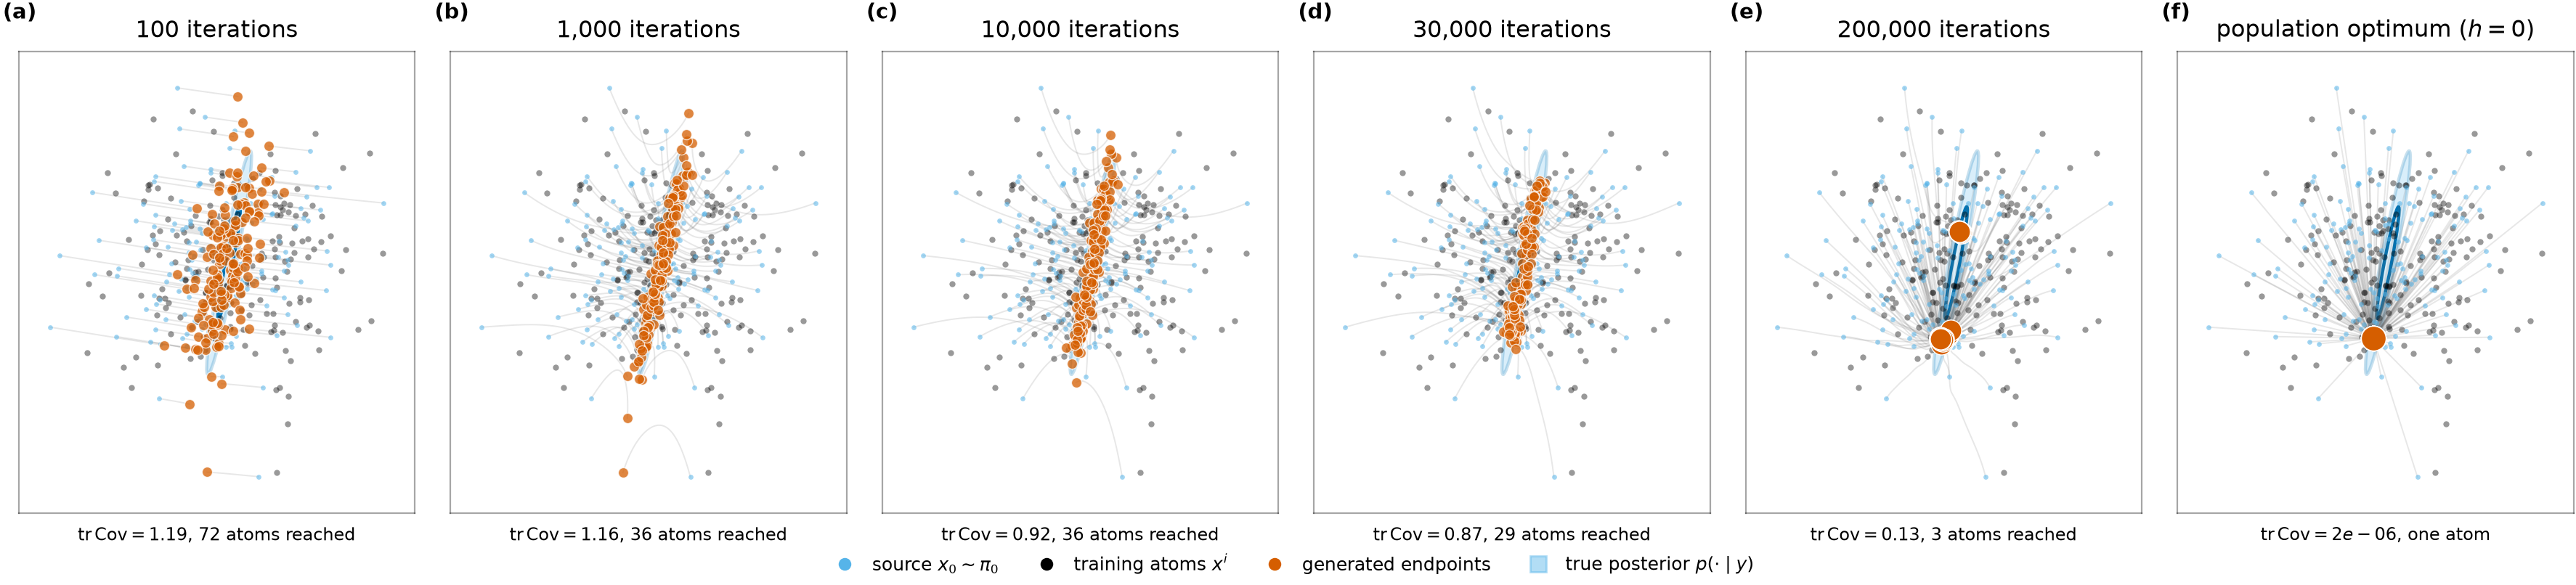
\includegraphics[width=\textwidth]{fig_collapse_training.png}
\caption{Conditional collapse as training proceeds (EXP-1, seed 0, $h{=}0$, one
condition). Panels (a--e) integrate the trained network at the iteration shown; panel
(f) integrates the exact population field, where every path lands on the labelled atom
and the conditional variance is zero. Each panel prints the trace of the generated
covariance and how many distinct training atoms the $160$ paths reach. Produced by
\texttt{scripts/make\_flow\_portraits.py}.}
\label{fig:traintraj}
\end{figure}

\paragraph{Measurement conventions dropped from the main text for space.} Every
across-seed $\pm$ in this paper is a \emph{population} standard deviation (denominator
$n$, not $n{-}1$), applied consistently throughout; at $n{=}5$ the sample standard
deviation is larger by $\sqrt{5/4}\approx1.12$, so a reader preferring that convention
should widen each interval by about $11\%$. On the CIFAR-10 DDPM run, the trace of a
covariance estimated from $M$ samples carries a relative sampling error of about
$\sqrt{2/(M-1)}$: $8.9\%$ at the $M{=}256$ used for evaluation but $36\%$ at the
$M{=}16$ logged during training, which is why every reported value is re-measured from
checkpoints. At $h{=}0$ the final $\tr\Cov$ is $0.431$ on the training-time estimator
and $0.458$ re-measured at $M{=}256$. And on the early-stopping measurement of
Appendix~\ref{app:remedies}: at $h{=}4$ the aggregate ratio never reaches $1$ within the
budget, falling only to $2.26$.

\begin{table}[t]
\centering\small
\begin{tabular}{ccccccc}
\toprule
$h$ & $n_{\mathrm{eff}}$ & median $\tr\Cov/\tr\Covh$ & $\beta$ (s.e.) & $R^2$ &
decades in $\tr\Covh$ & CV of $\tr\Covh$\\
\midrule
$4$ & $2.6$ & $5.30$ \,[$2.24$, $7.45$] & $0.481$ $(0.037)$ & $0.785$ & $4.57$ & $1.102$\\
$5$ & $16.4$ & $1.38$ \,[$1.18$, $1.78$] & $0.349$ $(0.049)$ & $0.522$ & $2.16$ & $0.537$\\
$6$ & $74.9$ & $1.15$ \,[$1.08$, $1.18$] & $-0.156$ $(0.058)$ & $0.135$ & $0.74$ & $0.208$\\
\bottomrule
\end{tabular}
\caption{CIFAR-10, DDPM U-Net, $48$ conditions at $M{=}256$. Brackets are $95\%$
bootstrap intervals for the median ratio. $\beta$ is the across-condition log--log
slope of measured against predicted variance (Fig.~\ref{fig:cifartrack}); theory
predicts $\beta=1$. The last two columns say how much range the regression had:
the number of decades spanned by the predictor and its coefficient of variation.}
\label{tab:cifarddpm}
\end{table}

\paragraph{The three supporting measurements of Section~\ref{sec:cifarddpm}.}
Atomicity, exact for the population minimiser, does not survive training: the fraction of
samples on a training atom is $1.000$, $0.829$, $0.717$, $0.620$ at $h=0,4,5,6$, the
exact $1.000$ at $h{=}0$ ruling out the integrator as the cause. What governs the
discrepancy is $n_{\mathrm{eff}}$ rather than $h$: pooled over the $144$ (condition,
$h$) pairs with $h>0$, Spearman's correlation is $-0.858$ against $n_{\mathrm{eff}}$ and
$-0.554$ against $h$. And three fresh problem instances separate the estimators sharply:
the average of per-condition ratios spreads by $281\%$ at $h{=}4$ against $23\%$ for the
aggregate ratio, since a per-condition denominator can be arbitrarily close to zero---but
even the aggregate survives only where the reference has range, the three instances
giving $1.181$, $0.924$ and $1.166$ at $h{=}6$.

Table~\ref{tab:exp1} reports the four exact-theory observables (curves in
Figure~\ref{fig:p1p4}, appendix). As training proceeds past
the good-calibration phase, the conditional generated variance collapses from
$\approx\Sigmapost$ toward $0$ (P1), the velocity field approaches the collapsed
closed form $(x^i-x)/(1-t)$ (P2), the generated mean moves from $\mu_{\mathrm{post}}$
toward the training point $x^i$ (P3), and the unconditional baseline retains
data-scale variance throughout (P4).



The variance tracks the true posterior up to $\sim\!10^4$ iterations---the model is a
correct Bayesian sampler in this phase, which is exactly why early stopping works
\citep{physicscfm2026}---and then collapses, stalling near $0.40$ at $2\times10^5$.
This residual is an \emph{optimisation} gap, not a failure of
Proposition~\ref{prop:collapse}: all four observables keep descending with the loss.
At a \emph{fixed} learning rate, however, training eventually diverges near $10^6$
iterations, since $(\star)$ steepens as $t\to1$ and a constant step becomes too large
once the loss is small. A cosine schedule ($\text{lr}:10^{-3}\to10^{-6}$) removes that
divergence on all 5 seeds. The cleanest evidence of deeper collapse is same-seed: at
the identical $7\times10^5$ checkpoint seed~0 reaches $\tr\Cov=0.128$ with the schedule
versus $0.162$ without, continuing to $0.115$ by $10^6$. The 5-seed mean
$0.120\pm0.054$ shows mainly that no seed diverges, \emph{not} a tight improvement on
$0.16$: seeds at $10^6$ range $0.035$--$0.186$, a spread inflated by the seed-conflated
problem instance, and only four of five improve from $7\times10^5$ to $10^6$.
Figure~\ref{fig:collapse2d} (appendix) shows the endpoint in sample space, with
per-condition $\tr\Cov$ spanning $5.8\times10^{-5}$ to $8.4\times10^{-2}$---collapse in
every condition, though not to equal depth.

\paragraph{A literature-standard memorisation ratio confirms Corollary~\ref{cor:distinction}.}
The diagnostics above are aggregate (a covariance trace, or distances of the sample
\emph{mean}). As a per-sample complement we report the \emph{memorisation ratio} of
\citet{yoon2023memorization}\footnote{As used, e.g., by \citet{buchanan2025edge}.}:
$\hat x$ is \emph{memorised} if $\|\hat x-x^{(1)}\|^2\le c\|\hat x-x^{(2)}\|^2$ for
$c=1/9$, with $x^{(1)},x^{(2)}$ the two nearest training points. Over 5 seeds both
flows rise from a common $\approx0.11$ baseline, the conditional reaching
$0.650\pm0.033$ at $2\times10^5$ versus $0.389\pm0.032$ unconditionally
(Figure~\ref{fig:memratio})---confirmation that \emph{both} memorise
(Corollary~\ref{cor:distinction}), conditionally more strongly. The two are not
comparable in magnitude---the unconditional target is spread over $N{=}200$ atoms, so
the $c{=}1/9$ test is mechanically harder there---so we read this directionally only.
The scheduled run reaches $0.955\pm0.020$ by $10^6$: 95\% of \emph{individual} samples
are memorised, not merely the sample mean.

\paragraph{Held-out labels: nearest-atom collapse, not generalisation.}
Corollary~\ref{cor:zerobw} predicts what the diagnostics above do not test: at a query
$y$ that is \emph{not} a training label the $h\to0$ endpoint is $\delta_{x^{i^\star}}$
for the nearest label $i^\star$, so held-out conditions should collapse too---onto a
memorised atom, not onto the correct posterior. Over 8 held-out $y$ per run this is
what happens: held-out $\tr\Cov$ tracks the training value (medians $0.43$ vs.\ $0.42$
at $2\times10^5$) while $\|\text{mean}-\mu_{\mathrm{post}}(y)\|$ grows from $0.12$ to
$0.87$ (median): overtraining moves the sampler away from the Bayes answer at
\emph{new} labels too.
We quote medians because in one of five seeds the held-out ODE \emph{diverges},
inflating the mean to $6\times10^4$ (Appendix~\ref{app:heldout}).


\paragraph{Adversarial pairing: collapse does not require a real posterior.}
Proposition~\ref{prop:collapse} never uses $A$ or $\sigma_{\mathrm{obs}}$---only that
the labels are pairwise distinct---so collapse should be unchanged if $Y$ is randomly
permuted relative to $X$ before training. It is: $\tr\Cov$ falls to $0.625\pm0.108$ at
$2\times10^5$ (vs.\ $0.396\pm0.127$ under the real pairing, an optimisation-difficulty
gap at fixed budget), while the distance to $y^i$'s \emph{true} posterior mean
\emph{grows}, $0.84\pm0.13\to1.437\pm0.176$, crossing above $\|\text{mean}-x^i\|$
between $10^4$ and $3\times10^4$ iterations. The generated law tracks the arbitrary
label-to-example assignment, not any statistical relation between $x$ and $y$
(Appendix~\ref{app:adv}).

This is our strongest empirical confirmation of the theory. The correct reference is
$\Covh$ (Theorem~\ref{thm:endpoint}, Proposition~\ref{prop:moments}), \emph{not}
$\Sigmapost$. Evaluating trained checkpoints against the exact kernel moments over 20
conditions ($M{=}1000$, 5 seeds), the generated variance tracks $\Covh$ at every
bandwidth: ratio-to-kernel $=1.002\pm0.050$, $0.994\pm0.039$ and $1.011\pm0.022$ at
$h=0.05,0.1,0.5$ (Figure~\ref{fig:p7summary}; Table~\ref{tab:p7kernel}, appendix,
gives all entries). This is a verification of the \emph{endpoint law}, stronger than
a velocity-field check. At $h{=}0.01$ the ratio is high and unstable
($1.308\pm0.376$) because $n_{\mathrm{eff}}\approx3.5$ leaves $\Covh$ near-degenerate
for many conditions; the ratio of mean traces, $0.673/0.583=1.15$, is closer to $1$.



A natural but mistaken reading is that $h\approx0.1$ ``perfectly restores'' the
posterior variance: $\tr\Cov$ merely crosses $\Sigmapost\approx1.02$ near $h{=}0.1$
because for this problem $\Sigmapost\approx\Covh|_{h=0.1}\approx1.00$---a coincidence.
The correct target is $\Covh$, which the model attains at \emph{every} $h$. The field
itself agrees: $v_\theta$ matches the kernel minimiser \eqref{eq:kernel-field}
$2$--$4\times$ better than the single-atom field $(\star)$ at every $h$, and the gap
widens with $h$ (Table~\ref{tab:dagger} and Figure~\ref{fig:kernel}, appendix).

\paragraph{Atomicity caveat (empirical confirmation of
Proposition~\ref{prop:atomicity}).} Even at the best-matching $h$ the generated law
remains atomic: $n_{\mathrm{eff}}\approx26/200$ at $h{=}0.1$ and $\approx102/200$ at
$h{=}0.5$, and the MMD to the analytic posterior falls with $h$ ($0.256\to0.012$) but
reaches zero at no $h$ (Appendix~\ref{sec:aux}). Matching variance is not recovering
the posterior.

\paragraph{How large is the atomicity floor, and does endpoint smoothing help?}
Unlike the MMD, the floor \eqref{eq:w2floor} is directly computable: at the EXP-1
configuration $F=0.0353$, i.e.\ $W_2\ge0.19$ but only $3.5\%$ of $\tr\Sigmapost$, and
the \emph{population-optimal} atomic law already reaches ${\rm MMD}=0.0089$---below the
trained model's $0.024$. Atomicity, though exact, is therefore \emph{not} what the MMD
curves measure; we correct that misreading in Appendix~\ref{sec:aux}. The reason is
instrumental: an RBF MMD at the median-heuristic bandwidth cannot resolve inter-atom
spacing, which is why an MMD that falls with $h$ says nothing about whether the
support is still atomic.

Does the obvious remedy help? Proposition~\ref{prop:tgtnoise} is exact: replacing the
endpoint by $x^I+\rho\xi$ makes the population endpoint law
$\sum_ip_i^{(h)}\N(x^i,\rho^2I_d)$, which is absolutely continuous, so the Wasserstein
floor \eqref{eq:w2floor} stops applying altogether. The obstruction is genuinely
removed. It does not follow that the law gets closer to the posterior, and swept over
$(h,\rho)$ at the population optimum it does not: the best cell of the entire sweep is
$h{=}0.5,\rho{=}0$ in \emph{both} metrics (${\rm MMD}=0.0089$, ${\rm OT}=0.106$), and at
that $h$ smoothing makes both worse (${\rm MMD}\to0.0123$, ${\rm OT}\to0.131$ at
$\rho{=}0.2$). At the smaller $h{=}0.1$ there is a nominal OT improvement,
$0.168\to0.158$, but the difference of $0.010$ sits below the $0.014$ that the same
estimator returns for two independent draws from the same posterior
(\texttt{scripts/verify\_ot\_resolution.py}), so it is not a measurement.
Smoothing buys continuity and pays for it in variance mismatch, and at the bandwidth
that matters the payment exceeds the purchase.

The remedy is not useless everywhere. Retraining EXP-1 at $N{=}50$---where the $d{=}2$
floor is largest, $F/\tr\Sigmapost=0.19$---with $h{=}0.1$ and $\rho\in\{0,0.3\}$, the
generated $\tr\Cov$ matches \eqref{eq:tgtendpoint}'s $\tr\Covh+d\rho^2$ to within
$3\%$ in both arms, the mean is unchanged, and the distance to the posterior does fall:
$1.49\times$ in MMD and $1.29\times$ in entropic OT, in the same direction in each seed
(Appendix~\ref{app:tgt}). So where the atoms are sparse enough for the floor to
dominate, filling the gaps helps a little. Table~\ref{tab:floor} sweeps $(d,N)$ and
adds the caveat that matters: the gain grows with the floor at fixed $d$ but
\emph{not} across $d$---at $d{=}10$ the floor is largest and the gain among the
smallest, since an isotropic $\rho$ cannot fill a high-dimensional gap without paying
$d\rho^2$. Endpoint smoothing is defeated by dimension, as kernel density estimation
is.

We state this correction plainly because an earlier version of this paper reported the
opposite. It read a $2.1\times$ population gain and a $2.5\times$ trained-model gain in
entropic OT against $1.2$--$1.5\times$ in MMD, and built on that gap an argument that
OT sees the atomic support where MMD cannot. Those OT numbers came from a Sinkhorn
implementation whose log-domain dual mixed two unit conventions; it scored two
independent draws from the same Gaussian at $3.34$ and a point mass against a standard
Gaussian at exactly $0$. It is corrected and pinned to three closed forms in
\texttt{scripts/verify\_sinkhorn.py}, and with it corrected the gap does not exist: at
$N{=}50$ the MMD gain is the \emph{larger} of the two. The argument that MMD cannot
resolve inter-atom spacing survives on its own evidence---the population-optimal atomic
law scores ${\rm MMD}=0.0089$, below the trained model's $0.024$, so an MMD of that size
is compatible with a purely atomic law---and needs no help from OT.

\paragraph{Interpolant noise does not help (Proposition~\ref{prop:prop17}).} With the
\emph{corrected} target \eqref{eq:c2target} (verified by four closed-form checks) the
generated variance is unchanged from that obtained with the mis-specified $X_1-X_0$
target ($0.367\pm0.146$ vs.\ $0.372\pm0.140$ at $\sigma{=}0.1$; Table~\ref{tab:p7i},
appendix) and stays far below the posterior---exactly as \eqref{eq:invariance}
predicts, the endpoint law being $\delta_{x^i}$ for every $\sigma$ whether or not the
target is correct.

The informative regime is $h{=}4$, where the reference moves over $4.57$ decades. There
$\beta=0.481\pm0.037$ with $R^2=0.785$ across $48$ conditions: the model preserves the
ordering the theory predicts, at half the predicted exponent.
This is a partial confirmation, but it is not a static one. Measuring the same slope
at each saved checkpoint (Figure~\ref{fig:betatraj}) shows $\beta$ near zero for the
first $8000$ iterations---the model does not track the reference at all---after which
it rises monotonically and is \emph{still rising} when the budget ends:
$-0.03,-0.03,-0.05,+0.12,+0.20,+0.39$ at $h{=}4$ and
$-0.06,-0.05,-0.07,-0.00,+0.17,+0.22$ at $h{=}5$ (at $M{=}96$ throughout, so the
comparison across checkpoints is like for like; the final $h{=}4$ value re-measured at
$M{=}256$ is the $0.481$ quoted above). Tracking the kernel reference is therefore
something the model \emph{learns}, and $0.481$ is where $60000$ iterations reached
rather than a ceiling of the model class. We are careful about what this does and does
not show: it establishes that the deficit is at least partly an optimisation gap and
not a fixed property of the parameterisation, and it does \emph{not} establish that
$\beta\to1$, which would need a budget we have not run. Three rival explanations for a
fixed exponent---an additive variance floor, a hard floor, and an affine map---were
fitted to the final checkpoint and all lose to the power law in log space
($R^2$ $0.42$, $0.24$, $0.28$ against $0.78$ at $h{=}4$), so an offset is not what is
happening. At $h{=}6$, $\beta$ never leaves zero, which is what the missing range
predicts. The trained model reproduces the ordering
Theorem~\ref{thm:endpoint} implies---which conditions have more posterior variance---and
compresses its dynamic range, by a factor that itself grows with the reference. We put
it that way deliberately. Theorem~\ref{thm:endpoint} describes the population
minimiser; a $35.75$M-parameter network at $60000$ iterations is not that minimiser, so
$\beta=0.481$ is a fact about how far the optimisation has come, not a refutation. The
theory predicts the destination, not the speed.

\paragraph{What governs the discrepancy is $n_{\mathrm{eff}}$, not $h$.}
Pooling all $144$ (condition, $h$) pairs with $h>0$, the Spearman correlation between
the ratio and the effective sample size $n_{\mathrm{eff}}=1/\sum_jp_j^2$ is $-0.858$,
against $-0.554$ for the correlation with $h$ itself. The bandwidth matters only through
how many training atoms it actually pools; conditions whose kernel weight concentrates on
one or two atoms are the ones the model overshoots, at any $h$.

\paragraph{Reproducibility across problem instances.} Every bandwidth was run at three
seeds, each redrawing the mask, the training subset and all training randomness, so
each seed is a different problem and not merely a different run: at $h{=}4$,
$n_{\mathrm{eff}}$ is $2.36$, $2.77$ and $2.10$ across the three. Table~\ref{tab:seed3}
gives the final values. Reading the spread as $(\max-\min)/\mathrm{mean}$: the raw
$\tr\Cov$ moves by $41\%$ at $h{=}4$, $23\%$ at $h{=}5$ and $16\%$ at $h{=}6$, while
the aggregate ratio $\tr\Cov/\tr\Covh$ moves by $23\%$, $30\%$ and $23\%$.

That is a narrower claim than an earlier version of this paper made, and we state the
change. With two seeds the aggregate ratio moved by $9.3\%$ at $h{=}4$ and $0.27\%$ at
$h{=}5$, and we concluded that the reference-relative quantity is the stable one. The
third seed shows the $h{=}5$ figure to have been a coincidence---two instances landed
on $1.245$ and $1.248$, the third on $1.654$---and at $h{=}5$ and $h{=}6$ the aggregate
ratio is in fact \emph{less} stable across instances than the raw trace it was meant to
stabilise. What survives is the case at $h{=}4$, where the ratio moves by $23\%$
against the raw trace's $41\%$; and $h{=}4$ is exactly the bandwidth at which the
reference has range across conditions, which is the same condition the $\beta$
measurement identifies as the informative one. A reference-relative statistic can only
stabilise what its denominator actually varies over.

At $h{=}6$ the three aggregate ratios are $1.181$, $0.924$ and $1.166$: a $23\%$ spread
that straddles $1$. So the apparent agreement there is not merely uninformative for
want of range---it is not stable even in the sign of its deviation, and a single-seed
reading could have been reported as agreement to $18\%$ or to $8\%$ depending on which
instance was drawn. At $h{=}0$, where the reference variance is exactly zero and the
ratio is undefined, $\tr\Cov$ is $0.431$, $0.409$ and $0.467$, a $13\%$ spread, and
$n_{\mathrm{eff}}=1.00$ at every condition of every seed.

\paragraph{Which ratio, and a third false certificate.} That conclusion depends on
\emph{how} the ratio is formed, and the difference is large enough to reverse it. The
aggregate ratio---$\tr\Cov$ summed over conditions divided by $\tr\Covh$ summed over
conditions---is what Theorem~\ref{thm:endpoint} predicts and what reproduces. The
average of per-condition ratios does not, and the three seeds make that beyond
argument: at $h{=}4$ they give $6.83$, $7.07$ and $307.7$, and at $h{=}5$ $2.315$,
$1.356$ and $37.17$. The reason is that a per-condition ratio has a denominator that
can be arbitrarily close to zero, so its average is heavy-tailed and dominated by
whichever condition happened to draw the smallest $\tr\Covh$---the same pathology that
makes the $M{=}256$ mean $20.4$ against a median of $5.30$ at $h{=}4$
(Section~\ref{sec:cifarddpm}). An earlier version of this paper argued
instance-stability from the two-seed $3.5\%$ figure alone; adding seeds turned that
$3.5\%$ into $281\%$. We report the aggregate ratio throughout,
and medians with bootstrap intervals where per-condition detail is needed.

\begin{figure}[htb]
\centering
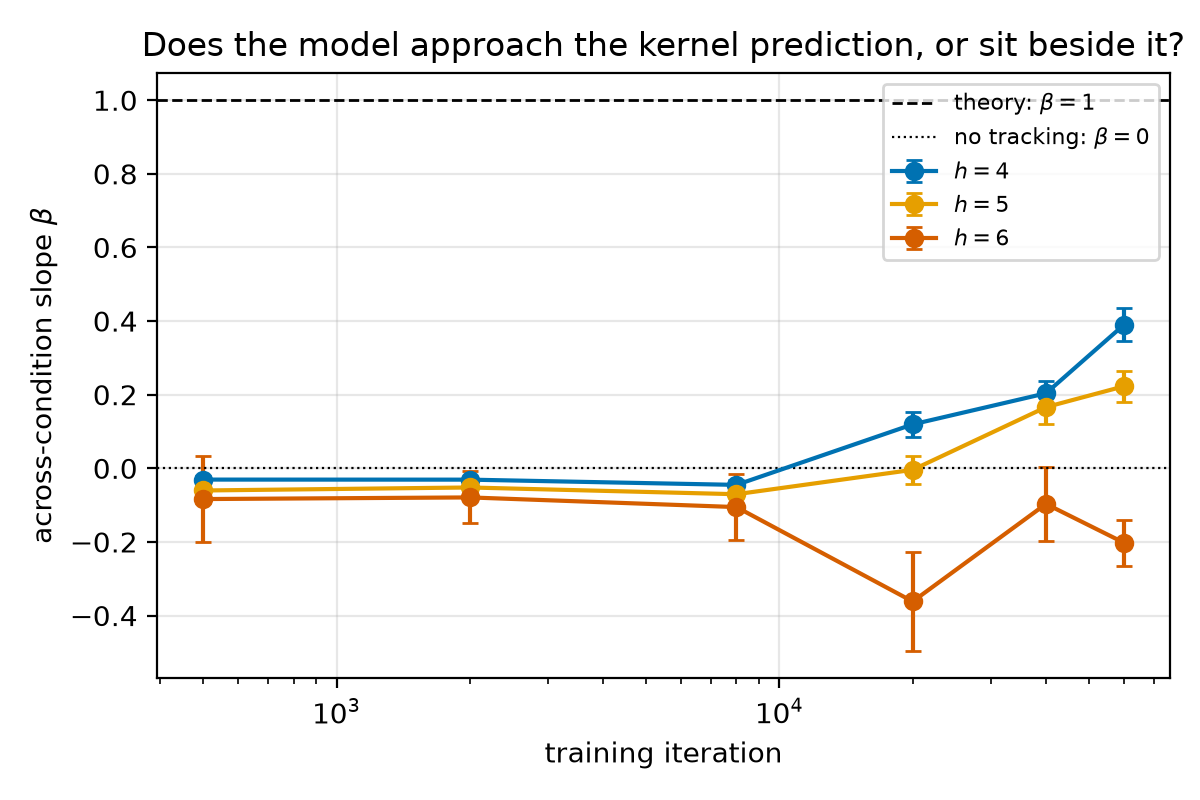
\includegraphics[width=0.62\textwidth]{fig_beta_trajectory.png}
\caption{The across-condition slope $\beta$ against training iteration, at $M{=}96$ per
condition. For the first $8000$ iterations the model does not track the kernel
reference at any bandwidth. After that $\beta$ rises at $h{=}4$ and $h{=}5$ and has not
levelled off by the end of the run, so the gap to the predicted $\beta=1$ is at least
partly an optimisation gap rather than a property of the model class. At $h{=}6$ it
stays at zero, which is what a reference with almost no range across conditions
predicts. Error bars are standard errors of the slope.}
\label{fig:betatraj}
\end{figure}

\begin{table}[htb]
\centering\small
\setlength{\tabcolsep}{4pt}
\begin{tabular}{cccccccc}
\toprule
& \multicolumn{4}{c}{$\tr\Cov$ \ / \ aggregate ratio $\tr\Cov/\tr\Covh$} &
\multicolumn{3}{c}{spread $(\max-\min)/\mathrm{mean}$}\\
\cmidrule(lr){2-5}\cmidrule(l){6-8}
$h$ & seed 0 & seed 1 & seed 2 & $n_{\mathrm{eff}}$ &
raw & aggregate & mean-of-ratios\\
\midrule
$0$ & $0.431$ & $0.409$ & $0.467$ & $1.00$ & $13.4\%$ & --- & ---\\
$4$ & $178.5$ / $2.255$ & $240.7$ / $2.463$ & $160.7$ / $1.944$ & $2.1$--$2.8$ &
  $41.4\%$ & $\mathbf{23.4\%}$ & $281\%$\\
$5$ & $276.8$ / $1.245$ & $321.2$ / $1.248$ & $349.0$ / $1.654$ & $13.0$--$17.2$ &
  $\mathbf{22.9\%}$ & $29.6\%$ & $263\%$\\
$6$ & $406.4$ / $1.181$ & $347.1$ / $0.924$ & $364.9$ / $1.166$ & $50$--$93$ &
  $\mathbf{15.9\%}$ & $23.5\%$ & $70.6\%$\\
\bottomrule
\end{tabular}
\caption{Three seeds of the CIFAR-10 DDPM sweep at $60000$ iterations, each a fresh
problem instance. Bold marks the more stable of the raw trace and the aggregate ratio
on each row. The aggregate ratio wins only at $h{=}4$, the bandwidth where the kernel
reference varies across conditions; where the reference is nearly constant, dividing by
it adds noise instead of removing it. The last column is why the paper does not use the
average of per-condition ratios anywhere: at $h{=}4$ the three seeds give $6.83$,
$7.07$ and $307.7$, the last carried by one condition whose reference happened to fall
near zero.}
\label{tab:seed3}
\end{table}

\subsection{The survival bound, measured (empirical)}
\label{app:survival}

\paragraph{The fourth case of Proposition~\ref{prop:survival}(d) is not vacuous.} The
spatially constant $\Delta(t)=c(1-t)^{-1}e^{i\theta(t)}$ in the plane, with
$\theta(t)=\log\frac1{1-t}$, gives $e_t=c\,e^{i\theta(t)}/(1+i)+O(1-t)$, so $|e_t|$
sits at $c/\sqrt2$ forever while its direction turns and never settles---critical
magnitude with no endpoint at all. \texttt{scripts/verify\_error\_survival.py} (part~F)
integrates the two flows and recovers $|e_t|=0.7071$ to five decimals.

\paragraph{Tightness of Corollary~\ref{cor:lossform}.} We report the bound's tightness
rather than assert it: over sixteen configurations---spatially constant and linear
errors, magnitudes growing like $(1-t)^{-a}$ for $a\in\{0,\tfrac12,1\}$, and two
truncations---it holds everywhere, with the measured deviation between $1.9$ and $27$
times below the bound (\texttt{scripts/verify\_error\_survival.py}). The slack tracks
$L_\Delta$, as the $e^{L_\Delta}$ factor says it should: it is smallest for errors
constant in space, where that factor is $1$, and largest for the steepest linear error
tested. So the bound is honest about the scaling $\sqrt{\mathcal L_i\delta}$ and loose
in its constant, and we use it for the former.

\paragraph{The scaling, tested on the runs themselves.} EXP-1 records both the training
loss and the retained conditional variance at every checkpoint, at a fixed sampler
truncation $\delta=10^{-3}$, so \eqref{eq:lossform} predicts $\log\sqrt{\tr\Cov}$ to be
affine in $\log\mathcal L_i$ with slope $\tfrac12$. Over the six checkpoints from $10^3$
iterations onward the measured slope is $0.429$ at $R^2=0.99$, and over the last
three---where collapse is actually running---it is $0.485$ at $R^2=0.998$
(Figure~\ref{fig:survival}(c), \texttt{scripts/verify\_error\_survival.py}). The two
earliest checkpoints are excluded and reported separately: at $10^2$ and
$3\times10^2$ iterations the model is still leaving its initialisation, holds data-scale
variance, and is not collapsing at all, so it is not in the regime the corollary
describes. The prefactor is $e^{L_\Delta}\approx25$ and is near-constant across the
collapse ($23.9\to26.0$), which is what the bound predicts for an error whose spatial
Lipschitz constant is not changing much; it holds here with $L_\Delta\ge3.2$, consistent
with the empirical Lipschitz constants of Figure~\ref{fig:lipschitz}. We put this no
more strongly than it deserves: the observed scaling is \emph{consistent} with the
$\tfrac12$ exponent the bound predicts, on one problem and one training trajectory,
which is not a demonstration that optimisation must follow it. The constant is loose by
a factor of $25$ and we do not use it at all. This is also where ``optimisation-paced''
stops being a turn of phrase and becomes a measurement.


\subsection{Architecture and optimiser sensitivity}

Every headline result in Section~\ref{sec:experiments} uses one fixed architecture
(4-layer, width-128 MLP, Adam). Since Proposition~\ref{prop:collapse}
constrains only the \emph{population} minimiser, not any parameterisation, the
theory predicts collapse for \emph{any} sufficiently expressive architecture; what
it does not predict is how fast a given architecture and optimiser reach it within
a fixed iteration budget. We re-ran EXP-1 (conditional, $2$ seeds each) varying one
factor at a time---width $\in\{32,64,256\}$ at depth $4$, depth $\in\{2,6\}$ at
width $128$, and the optimiser (SGD with momentum $0.9$, $\text{lr}=10^{-2}$, in
place of Adam)---holding everything else, including the $2\times10^5$-iteration
budget, fixed.

Table~\ref{tab:ablation} reports the result. None of these variants contradicts
Proposition~\ref{prop:collapse}: all seven configurations collapse monotonically from
the same $\approx\tr\Sigmapost$ starting point (not shown), and none plateaus above
the baseline's level by more than a factor of $\sim\!2$---exactly the qualitative
picture the theory predicts (every sufficiently expressive architecture converges
toward the same population optimum) together with the optimisation-gap caveat of
Section~\ref{sec:limitations} (how close a given budget gets you depends on the
architecture and optimiser). We did not extend this sweep to the Lipschitz
diagnostic of Appendix~\ref{sec:aux} or to EXP-2/EXP-3; doing so is left to future
work.

\begin{table}[htb]
\centering\small
\begin{tabular}{lcccc}
\toprule
configuration & width & depth & optimiser & $\tr\Cov$ at $2\times10^5$ \\
\midrule
baseline & 128 & 4 & Adam & $0.396\pm0.127$ \\
\midrule
narrower & 32 & 4 & Adam & $0.657\pm0.058$ \\
         & 64 & 4 & Adam & $0.526\pm0.058$ \\
wider    & 256 & 4 & Adam & $0.403\pm0.079$ \\
shallower& 128 & 2 & Adam & $0.860\pm0.156$ \\
deeper   & 128 & 6 & Adam & $0.407\pm0.127$ \\
SGD      & 128 & 4 & SGD(m=0.9) & $0.711\pm0.193$ \\
\bottomrule
\end{tabular}
\caption{Architecture/optimiser ablation on EXP-1 (2 seeds each), same
$2\times10^5$-iteration budget as Table~\ref{tab:exp1}. Collapse speed increases
with capacity but saturates beyond roughly the baseline's size (width $256$ and
depth $6$ both land within seed noise of the width-$128$/depth-$4$ baseline,
despite reaching a strictly lower training loss---$0.46$ vs.\ $0.59$ for width
$256$---so more capacity buys a better loss without a proportionally deeper
collapse at this budget); under-capacity architectures (width $32$, depth $2$)
collapse markedly less within the same budget; and the optimiser matters
substantially, with SGD reaching only about half the collapse Adam does here.}
\label{tab:ablation}
\end{table}


\subsection{Adversarial pairing: collapse does not require a real posterior}
\label{app:adv}
\label{sec:adversarial}

Proposition~\ref{prop:collapse} never uses $A$ or $\sigma_{\mathrm{obs}}$: it needs
only that $y^1,\dots,y^N$ be pairwise distinct. It therefore predicts that collapse
is unchanged if $Y$ is \emph{randomly permuted relative to $X$} before training, so
that $(x^i,y^i)$ is no longer the true generative pair---identification, not
discovered posterior structure. This mirrors the ``Adversarial Pairings'' experiment
of \citet{gradvar2025} (shuffled OT-coupling targets on CelebA, unconditional),
adapted to the conditional case where the prediction is exact.
Re-running EXP-1 unchanged (5 seeds), permuting $Y$ independently per seed,
$\tr\Cov$ collapses under shuffled labels just as under the real pairing, from
$\gtrsim1$ to $0.625\pm0.108$ at $2\times10^5$ (vs.\ $0.396\pm0.127$ real); the gap
is optimisation difficulty at a fixed budget---a random $x$--$y$ pairing is a harder
target to fit---not a difference in the population optimum, which
Proposition~\ref{prop:collapse} fixes at $0$ either way. The sharper diagnostic is
$\|\text{mean}-\mu_{\mathrm{post}}(y^i)\|$, the distance to $y^i$'s \emph{true}
analytic posterior mean (still computable from $A$, but now unrelated to the $x^i$
the label was shuffled onto): it does not shrink but \emph{grows} throughout
training, $0.84\pm0.13\to1.437\pm0.176$, crossing above
$\|\text{mean}-x^i\|$ ($1.35\pm0.10\to0.559\pm0.104$) between $10^4$ and
$3\times10^4$ iterations and staying above it thereafter
(Figures~\ref{fig:adv-trace}--\ref{fig:adv-mean}, appendix). The generated law
tracks the arbitrary label-to-example assignment, not any statistical relationship
between $x$ and $y$---Corollary~\ref{cor:distinction}'s conclusion, confirmed even
when the labels carry no real information about $x$ at all.


\begin{figure}[htb]
\centering
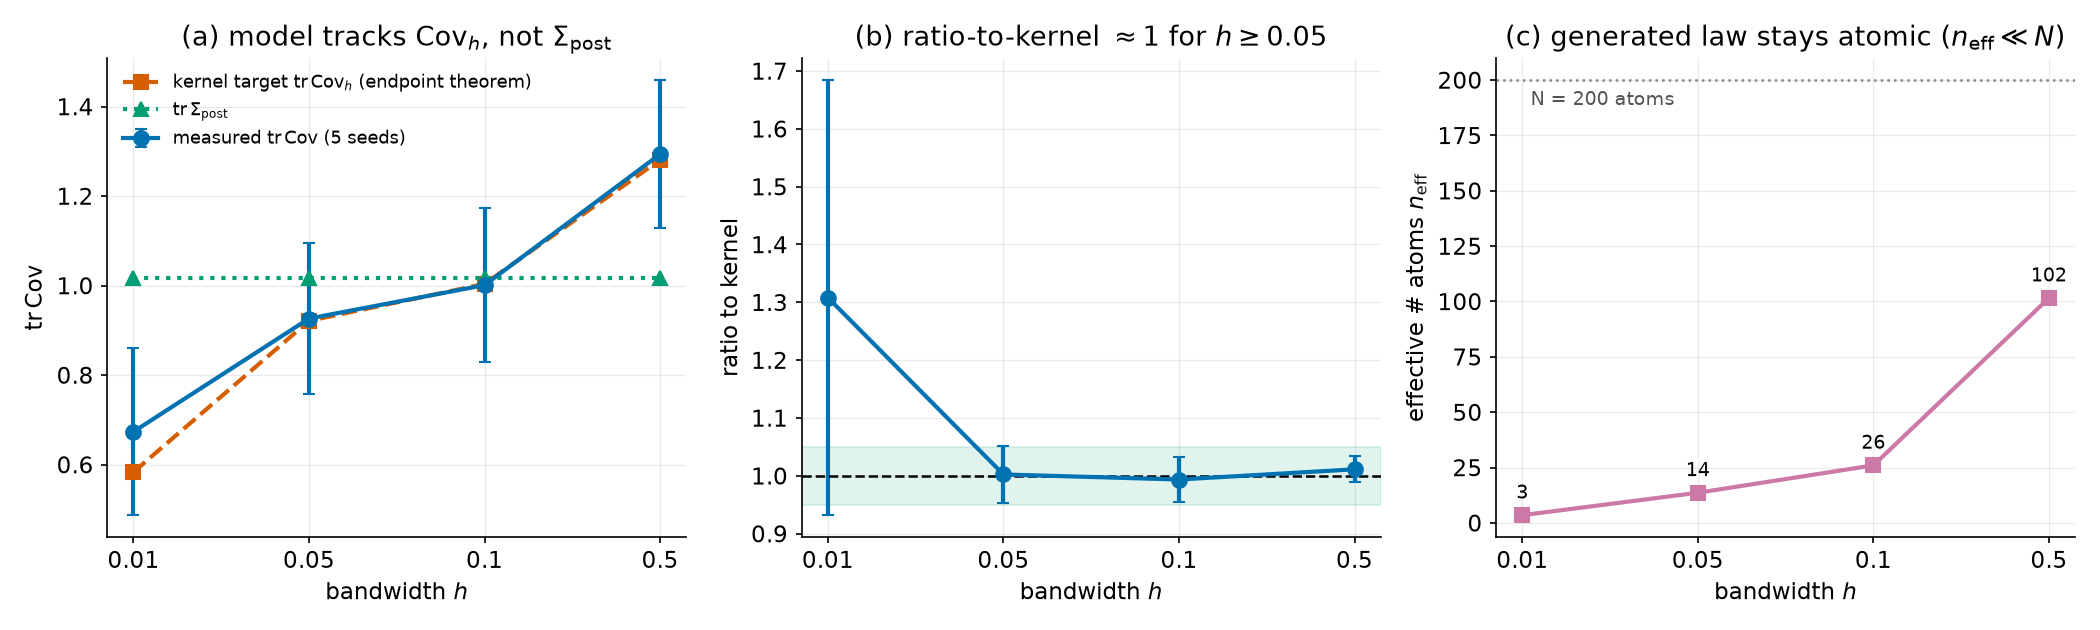
\includegraphics[width=0.96\textwidth]{fig_p7_summary.png}
\caption{P7 headline (5 seeds, error bars over seeds). \textbf{(a)} Generated
$\tr\Cov$ follows the kernel target $\tr\Covh$ (dashed) and crosses $\tr\Sigmapost$
(dotted) only incidentally near $h{=}0.1$. \textbf{(b)} Ratio-to-kernel stays in the
shaded $[0.95,1.05]$ band for $h\ge0.05$. \textbf{(c)} $n_{\mathrm{eff}}\ll N$: a
sparse mixture of atoms (Proposition~\ref{prop:atomicity}), not a continuous
posterior.}
\label{fig:p7summary}
\end{figure}

Figure~\ref{fig:bandwidthportrait} is the same statement in trajectory space, for one
condition: the reference law at each bandwidth above, and the network trained at that
bandwidth below. As $h$ grows the reference spreads over more atoms
($n_{\mathrm{eff}}=1,4,18,81$) and the trained model follows it, at ratios of $1.24$,
$1.09$ and $1.12$ on this condition---noisier than the $1.002\pm0.050$,
$0.994\pm0.039$, $1.011\pm0.022$ of Figure~\ref{fig:p7summary}, which averages $20$
conditions and $5$ seeds at $M{=}1000$ where this draws $160$ paths through a single
condition, for which the trace alone carries an $11\%$ sampling error.

\begin{figure}[htb]
\centering
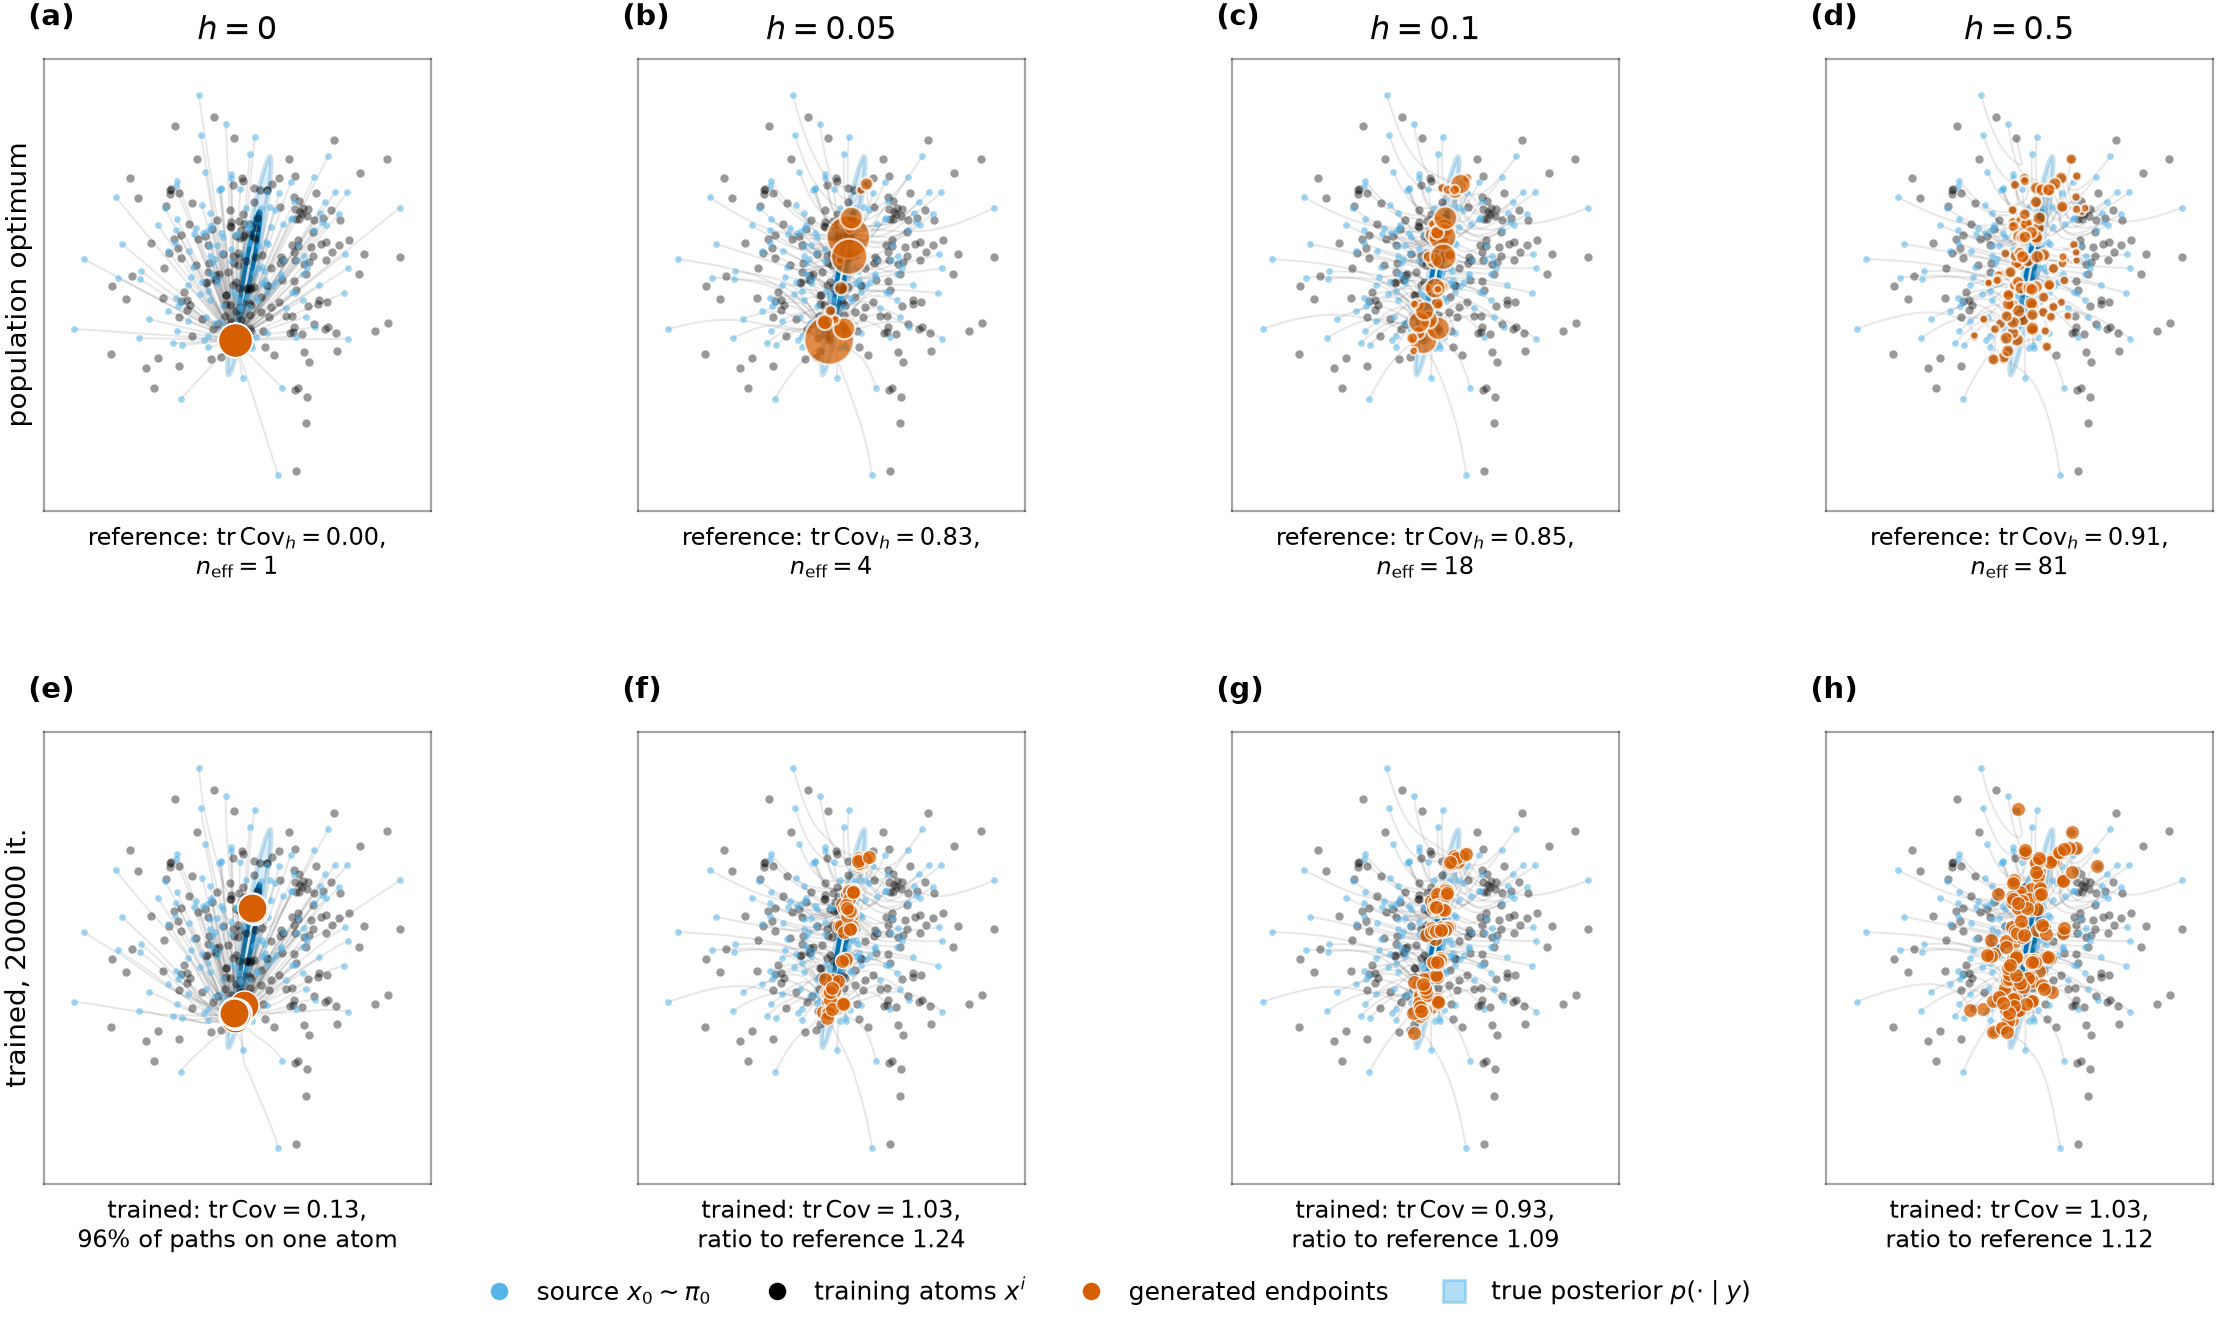
\includegraphics[width=0.92\textwidth]{fig_bandwidth_portrait.png}
\caption{Label smoothing as a flow, at four bandwidths, on one condition of the EXP-1
instance. \textbf{Top:} the exact population endpoint law of
Theorem~\ref{thm:endpoint}, marker area $\propto p^{(h)}_i$; at $h{=}0$ it is one atom,
and widening $h$ reweights the \emph{same} atoms, never adding new ones. \textbf{Bottom:}
an MLP trained at that same bandwidth for $200000$ iterations, integrated from the same
$160$ draws of $x_0$. The model is converging to the law above it, not to some other
law: at $h{=}0$ it puts $96\%$ of its paths on the labelled atom, and at $h>0$ its trace
is within a quarter of the reference on a measurement whose own sampling error is
$11\%$. Produced by \texttt{scripts/make\_flow\_portraits.py}; the $h>0$ runs are
\texttt{p7yck\_h*\_seed0}, retrained for this figure because the original P7 sweeps kept
their metrics but not their checkpoints.}
\label{fig:bandwidthportrait}
\end{figure}

\subsection{The atomicity floor, measured}
\label{app:floor}

Table~\ref{tab:floor} evaluates the \emph{population} endpoint laws of
Theorem~\ref{thm:endpoint} and Proposition~\ref{prop:tgtnoise} directly, so it bounds
what any trained model could achieve and is independent of optimisation. For each
$(d,N)$ we draw the analytic posterior at six training labels, compute the floor
$F=\E_{x\sim p(\cdot\mid y)}\operatorname{dist}(x,\{x^i\})^2$ of \eqref{eq:w2floor}
exactly, and report the best MMD to that posterior over $h$ (atomic, $\rho=0$) and
over $(h,\rho)$ (endpoint-smoothed). Script:
\texttt{scripts/atomicity\_scaling.py}; the single-configuration sweep behind the
numbers quoted in Section~\ref{sec:p7} is \texttt{scripts/verify\_target\_noise.py}.

\begin{table}[htb]
\centering\small
\setlength{\tabcolsep}{4.5pt}
\begin{tabular}{ccccccccccc}
\toprule
& & & & & \multicolumn{2}{c}{MMD} & \multicolumn{3}{c}{entropic OT}\\
\cmidrule(lr){6-7}\cmidrule(l){8-10}
$d$ & $N$ & $\tr\Sigmapost$ & floor $F$ & $F/\tr\Sigmapost$ &
atomic & gain from $\rho$ & atomic & gain from $\rho$ & \emph{est.\ floor}\\
\midrule
2 & 1000 & 1.004 & 0.0073 & 0.007 & 0.0048 & $1.01\times$ & 0.08 & $1.01\times$ & \emph{0.020}\\
2 & 200  & 1.004 & 0.0353 & 0.035 & 0.0115 & $1.02\times$ & 0.18 & $1.09\times$ & \emph{0.014}\\
2 & 50   & 1.004 & 0.1932 & 0.192 & 0.0742 & $\mathbf{1.24\times}$ & 0.76 & $1.04\times$ & \emph{0.019}\\
5 & 200  & 4.001 & 0.9242 & 0.231 & 0.0059 & $1.05\times$ & 1.45 & $1.33\times$ & \emph{0.623}\\
10 & 200 & 9.001 & 4.8303 & 0.537 & 0.0105 & $1.07\times$ & 7.48 & $1.21\times$ & \emph{4.273}\\
10 & 50  & 9.001 & 7.0125 & 0.779 & 0.0434 & $1.18\times$ & 12.72 & $1.23\times$ & \emph{4.273}\\
\bottomrule
\end{tabular}
\caption{The atomicity obstruction, quantified at the population optimum. $F$ is the
exact bound of \eqref{eq:w2floor}, computed in closed form and so free of any
estimator; its relative size follows the $N^{-2/d}$ nearest-atom scaling. ``Gain from
$\rho$'' is the best score over $h$ alone divided by the best over $(h,\rho)$. The
last column is what the OT estimator returns for two independent $M$-sample draws
from the \emph{same} posterior (\texttt{scripts/verify\_ot\_resolution.py}): the
divergence does not vanish at finite $M$, and a difference smaller than that floor is
not a measurement. Read against it, the OT \emph{levels} are resolved on every
row---by $4$ to $40\times$ at $d{=}2$ and by $1.8$ to $2.3\times$ in higher
dimension---and they confirm that the atomic law's distance to the posterior grows
with $F$. The OT \emph{gains}, however, are $0.00$--$2.35$ in absolute terms against
floors of $0.014$--$4.27$, so they are below resolution at every row and we do not
read them; the endpoint-smoothing gain is taken from the MMD column, which needs no
such correction. One reading survives and is the one that matters: at fixed $d{=}2$
the MMD gain grows monotonically with the floor ($1.01\to1.02\to1.24\times$ as $N$
falls from $1000$ to $50$), but \emph{across} $d$ it does not---$d{=}10$ has the
largest floors and among the smallest gains ($1.07$, $1.18\times$)---because an
isotropic $\rho$ cannot fill a high-dimensional gap without paying $d\rho^2$ in
variance. Endpoint smoothing is
defeated by dimension, exactly as kernel density estimation is. The OT column uses a
coarser $(h,\rho)$ grid and $M{=}400$, so its absolute values are not comparable to
the $M{=}800$ single-configuration sweep quoted in Section~\ref{sec:p7}---which is also
why that sweep's floor, quoted there, is the tighter $0.014$.}
\label{tab:floor}
\end{table}

\subsection{Endpoint smoothing on a trained model, per seed}
\label{app:tgt}

Table~\ref{tab:tgt} gives the per-seed numbers behind the trained-model claim of
Section~\ref{sec:p7}. Both arms use the EXP-1 architecture and schedule unchanged at
$N{=}50$ and $h{=}0.1$, differing only in $\rho$
(\texttt{configs/exp1\_target\_noise.yaml}, \texttt{train.target\_noise\_rho});
analysis by \texttt{scripts/analyze\_target\_noise.py}. The measured $\tr\Cov$ tracks
$\tr\Covh+d\rho^2$ per seed as well as on average, and the improvement in both
distances is in the same direction in each seed separately---the aggregate is not
carried by one run. Seed variation is large in absolute terms (seed 0's problem
instance is markedly harder than seed 1's), which is why the ratio, not the level, is
the quantity to read.

\begin{table}[htb]
\centering\small
\begin{tabular}{llccccc}
\toprule
arm & seed & $\tr\Cov$ & predicted $\tr\Covh+d\rho^2$ & MMD & entropic OT &
$\|\text{mean}-\mu_{\mathrm{post}}\|$\\
\midrule
$\rho=0$   & 0 & 0.2176 & 0.2108 & 0.2330 & 0.905 & 0.5176\\
           & 1 & 0.4353 & 0.4436 & 0.1168 & 0.479 & 0.2790\\
           & \emph{mean} & \emph{0.3265} & \emph{0.3272} & \emph{0.1749} & \emph{0.692} & \emph{0.3983}\\
\midrule
$\rho=0.3$ & 0 & 0.3959 & 0.3908 & 0.1549 & 0.711 & 0.5383\\
           & 1 & 0.5870 & 0.6236 & 0.0798 & 0.364 & 0.2948\\
           & \emph{mean} & \emph{0.4914} & \emph{0.5072} & \emph{0.1174} & \emph{0.537} & \emph{0.4166}\\
\bottomrule
\end{tabular}
\caption{Endpoint smoothing in a trained model ($N{=}50$, $h{=}0.1$, $2\times10^5$
iterations, 8 conditions, $M{=}800$). The generated covariance matches
\eqref{eq:tgtendpoint}'s $\tr\Covh+d\rho^2$ to within $3\%$ in both arms, and the mean
is unchanged by $\rho$---both as the moment formula requires. Distance to the analytic
posterior falls $1.49\times$ in MMD and $1.29\times$ in entropic OT. An earlier version
of this table reported the OT column two orders of magnitude larger and falling
$2.5\times$, and read a metric-sensitivity argument off the gap between the two
columns. Those OT numbers came from a Sinkhorn implementation whose log-domain dual
mixed two unit conventions; it is corrected here, pinned to three closed forms in
\texttt{scripts/verify\_sinkhorn.py}, and the gap it appeared to show does not exist.
Endpoint smoothing helps in both metrics at this $N$ and this $h$, and by a similar
factor in each.}
\label{tab:tgt}
\end{table}

\subsection{Held-out conditions, per seed}
\label{app:heldout}

Table~\ref{tab:heldout} gives the per-seed numbers behind the held-out paragraph of
Section~\ref{sec:exp1}. Four of the five seeds behave alike---held-out $\tr\Cov$ ends
within a factor of $\sim\!2$ of the training-condition value, i.e.\ the same collapse,
onto the nearest memorised atom rather than onto the posterior of that $y$
(Corollary~\ref{cor:zerobw}). Seed 0 is the exception: its held-out ODE integration
diverges between $10^5$ and $2\times10^5$ iterations, which is why we report medians
in the main text. We did not investigate whether this divergence is a property of that
problem instance (the seed also draws $A$) or of the integrator's fixed step count
near $t{=}1$; distinguishing the two would need a step-size sweep we did not run.

\begin{table}[htb]
\centering\small
\begin{tabular}{lccccccc}
\toprule
& \multicolumn{5}{c}{per seed, $\tr\Cov$ at $2\times10^5$} & \multicolumn{2}{c}{5-seed}\\
\cmidrule(lr){2-6}\cmidrule(l){7-8}
group & 0 & 1 & 2 & 3 & 4 & mean & median\\
\midrule
training conditions & 0.407 & 0.547 & 0.450 & 0.417 & 0.162 & 0.396 & 0.417\\
held-out conditions & $3.0{\times}10^{5}$ & 0.212 & 0.429 & 0.364 & 0.564 & $6.0{\times}10^{4}$ & 0.429\\
\bottomrule
\end{tabular}
\caption{Held-out vs.\ training conditions at $2\times10^5$ iterations (8 held-out
$y$ per run). Four seeds collapse on held-out labels much as on training labels; seed
0's held-out integration diverges, making the 5-seed mean uninformative. Up to $10^5$
iterations no seed diverges and the two groups agree closely (held-out $0.51$ vs.\
training $0.58$).}
\label{tab:heldout}
\end{table}

\subsection{Scope-marked sweeps (P5, P6, $d/k$; empirical)}
\label{sec:sweeps}

The following depend on $N$ and $\sigma_{\mathrm{obs}}$ at fixed architecture and are
\emph{not} determined by the population theory (Section~\ref{sec:scope}); we report
them as empirical findings using the collapse ratio $\tr\Cov/\tr\Sigmapost$ at
$2\times10^5$ iterations (Tables~\ref{tab:sweeps}--\ref{tab:p5} and
Figure~\ref{fig:sweeps}).

\begin{table}[htb]
\centering\small
\begin{minipage}{0.48\textwidth}\centering
\begin{tabular}{lcccc}
\toprule
$N$ & 50 & 200 & 1000 & 5000\\
\midrule
ratio & $0.049$ & $0.389$ & $0.912$ & $0.990$\\
$\pm$ & $0.038$ & $0.123$ & $0.103$ & $0.031$\\
\bottomrule
\end{tabular}
\subcaption{P6: collapse vs.\ dataset size.}
\end{minipage}\hfill
\begin{minipage}{0.48\textwidth}\centering
\begin{tabular}{lccc}
\toprule
$(d,k)$ & $(2,1)$ & $(10,1)$ & $(10,10)$\\
\midrule
ratio & $0.390$ & $0.317$ & $0.0065$\\
$\pm$ & $0.127$ & $0.033$ & $0.0024$\\
\bottomrule
\end{tabular}
\subcaption{Collapse vs.\ dimension/observation.}
\end{minipage}
\caption{5-seed sweeps (empirical). P6 is monotone and stable across seeds: small $N$
collapses almost completely, $N{=}5000$ barely collapses ($\approx$ true posterior)---a
representation/optimisation statement, not a contradiction of
Proposition~\ref{prop:collapse}. Larger $k$ (a more informative label) sharpens the
identifier and deepens collapse, consistent with the identification mechanism.}
\label{tab:sweeps}
\end{table}

\begin{table}[htb]
\centering\small
\begin{tabular}{lcccc}
\toprule
$\sigma_{\mathrm{obs}}$ & 0.01 & 0.1 & 0.5 & 1.0\\
\midrule
$\tr\Sigmapost$ & 1.000 & 1.018 & 1.266 & 1.531\\
generated $\tr\Cov$ & $0.472\pm0.108$ & $0.396\pm0.127$ & $0.416\pm0.155$ & $0.507\pm0.236$\\
collapse ratio & 0.472 & 0.390 & 0.328 & 0.331\\
\bottomrule
\end{tabular}
\caption{P5 (empirical), 5 seeds. The between-$\sigma_{\mathrm{obs}}$ spread in the
ratio ($0.33$--$0.47$, range $\sim0.14$) is \emph{smaller} than the between-seed std
at each point ($0.11$--$0.24$): the sweep is flat within seed noise. This is
consistent with an identification-through-$y$ mechanism that operates for every
$\sigma_{\mathrm{obs}}>0$; the theory implies no monotonicity, so flatness is not a
falsification.}
\label{tab:p5}
\end{table}

\begin{figure}[htb]
\centering
\begin{subfigure}{0.48\textwidth}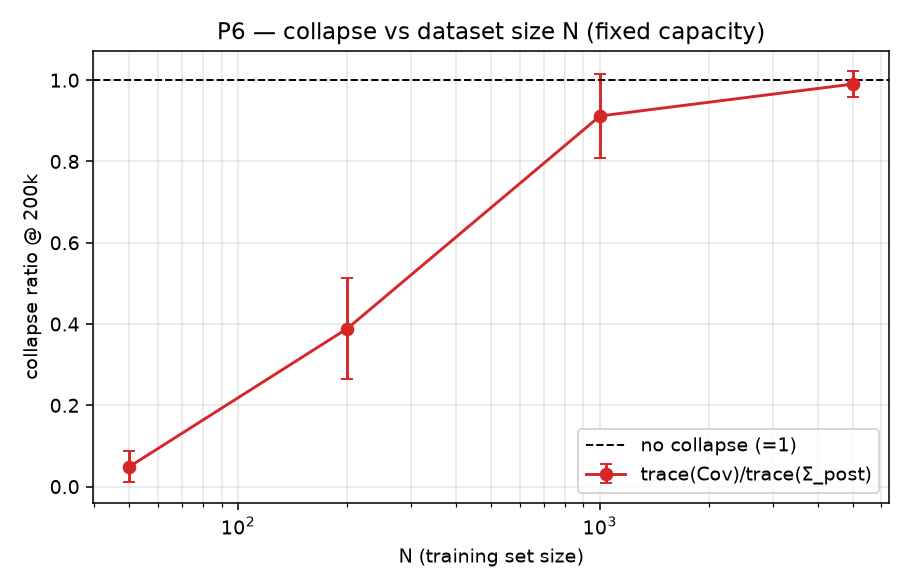
\includegraphics[width=\linewidth]{fig_p6_n.png}
\caption{P6: collapse ratio vs.\ dataset size $N$.}\end{subfigure}\hfill
\begin{subfigure}{0.48\textwidth}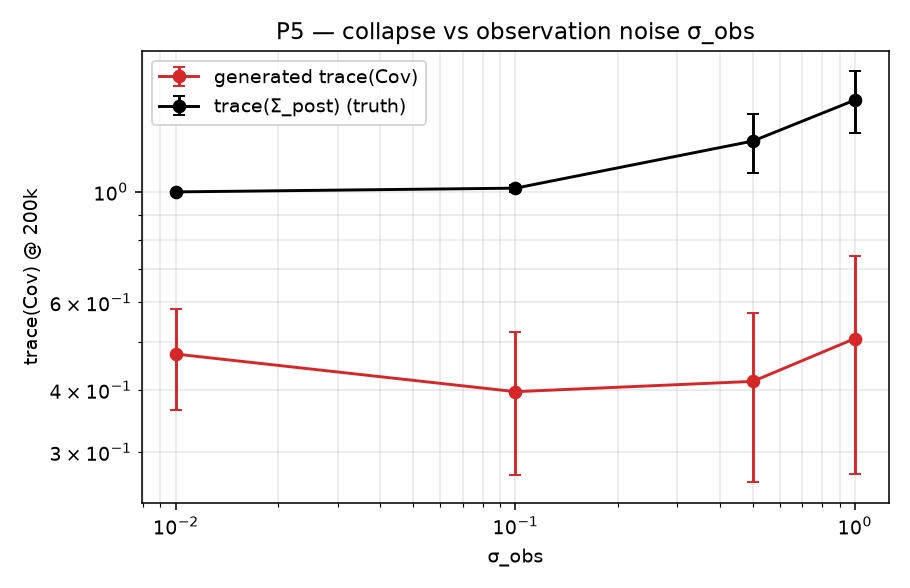
\includegraphics[width=\linewidth]{fig_p5_sigma.png}
\caption{P5: generated $\tr\Cov$ and $\tr\Sigmapost$ vs.\ $\sigma_{\mathrm{obs}}$
(their ratio is the collapse ratio of Table~\ref{tab:p5}).}\end{subfigure}
\caption{Scope-marked sweeps (5 seeds, error bars over seeds). Collapse deepens
monotonically as $N$ shrinks (a); it is flat within seed noise across
$\sigma_{\mathrm{obs}}$ (b). Neither is determined by the population theory; both are
reported as empirical findings (Section~\ref{sec:scope}).}
\label{fig:sweeps}
\end{figure}


\subsection{The same exposure control on EXP-1 (empirical)}
\label{sec:p6exposure}

The EXP-3 $N$-sweep of Appendix~\ref{sec:nsweep3} showed that a fixed-budget sweep
confounds $N$ with per-image exposure. The P6 sweep of Table~\ref{tab:sweeps} has
exactly the same design---every $N$ trained for $2\times10^5$ iterations at batch
$256$, so each training point receives $2\times10^5\cdot256/N$ gradient samples,
precisely proportional to $1/N$---and therefore the same confound. We rerun it holding
exposure fixed instead, at $51200$ gradient samples per training point (the value the
published $N{=}1000$ run happens to have), which means $10^4$ iterations at $N{=}50$ and
$10^6$ at $N{=}5000$; five seeds per point, $20$ runs.

\begin{table}[htb]
\centering\small
\begin{tabular}{lcccc}
\toprule
$N$ & 50 & 200 & 1000 & 5000\\
\midrule
iterations (fixed exposure) & $10^4$ & $4{\times}10^4$ & $2{\times}10^5$ & $10^6$\\
fixed budget ($2{\times}10^5$ iters) & $0.049\pm0.038$ & $0.389\pm0.123$ &
  $0.912\pm0.103$ & $0.990\pm0.031$\\
fixed exposure ($51200$/point) & $0.444\pm0.196$ & $0.774\pm0.165$ &
  $0.928\pm0.087$ & $1.014\pm0.065$\\
\bottomrule
\end{tabular}
\caption{P6 read two ways, collapse ratio $\tr\Cov/\tr\Sigmapost$, 5 seeds each.
Spread across $N$ falls from $20.2\times$ at fixed budget to $2.28\times$ at fixed
exposure. At fixed budget each point of the $N{=}50$ run sees $1024000$ gradient
samples against $10240$ for $N{=}5000$, a factor of $100$.}
\label{tab:p6exposure}
\end{table}

\begin{figure}[htb]
\centering
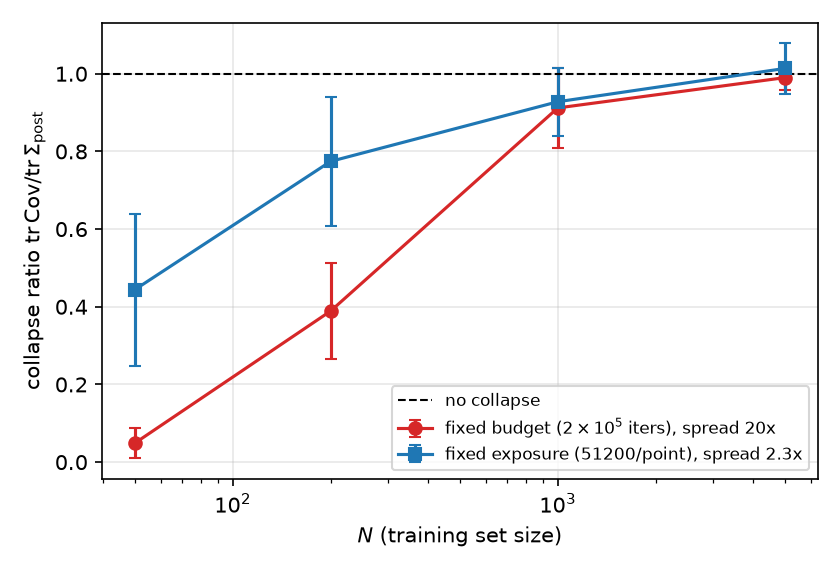
\includegraphics[width=0.62\textwidth]{fig_p6_exposure.png}
\caption{The P6 sweep read both ways. At a fixed iteration budget each training
point of the $N{=}50$ run receives a hundred times the gradient samples of the
$N{=}5000$ run, so ``collapse deepens as $N$ falls'' and ``collapse deepens as each
point is trained on more'' are the same curve. Holding exposure fixed instead
separates them, and most of the apparent $N$-dependence goes with it: the spread
across $N$ falls from $20.2\times$ to $2.28\times$, and $N{=}5000$ does not collapse
at all within the budget.}
\label{fig:p6exposure}
\end{figure}

Table~\ref{tab:p6exposure} reads the sweep both ways. Spread across $N$ falls from
$20.2\times$ to $2.28\times$ (Figure~\ref{fig:p6exposure}), and $N{=}5000$ reaches
$1.014$---no collapse at all within the budget. This replicates the EXP-3 finding
($14.9\times\to2.34\times$) on a different architecture, a different dimension and a
different dataset, which is the strongest form the claim can take here: two experiments
sharing none of those agree that the genuine $N$-dependence is a factor of about two,
not fifteen. Both the EXP-1 P6 sweep and the EXP-3 $N$-sweep as originally reported are
therefore statements about how far a fixed budget gets you at each $N$. We keep the
original numbers in Table~\ref{tab:sweeps} rather than replacing them, since they are
what the fixed-budget protocol yields and the comparison is the point.

\subsection{What the EXP-1 error bars are measuring (empirical)}
\label{sec:seedsplit}

Section~\ref{sec:experiments} notes that \texttt{seed} drives both the problem instance
(the operator $A$, hence $\Sigmapost$, and the dataset draw) and all training
randomness, so every $\pm$ in this paper mixes the two. A separate
\texttt{problem\_seed} makes them independent. Two sweeps of ten runs each at $2\times
10^5$ iterations---one holding the instance fixed and varying the run, one the
reverse---give the split.

\begin{table}[htb]
\centering\small
\begin{tabular}{llcccc}
\toprule
varying & held fixed & $n$ & mean & std & range\\
\midrule
training run & problem instance & 10 & 0.3363 & $0.0675$ & $[0.2477, 0.4500]$\\
problem instance & training run & 10 & 0.3986 & $0.1261$ & $[0.1819, 0.5580]$\\
\bottomrule
\end{tabular}
\caption{Decomposition of the EXP-1 error bar, collapse ratio at the final
checkpoint; sample standard deviations ($n{-}1$). Added in quadrature the two give
$0.1431$, against the published 5-seed spread of $0.123$ (population convention;
$0.1375$ on the sample convention)---a consistency check on the decomposition, not
only a measurement.}
\label{tab:seedsplit}
\end{table}

\begin{figure}[htb]
\centering
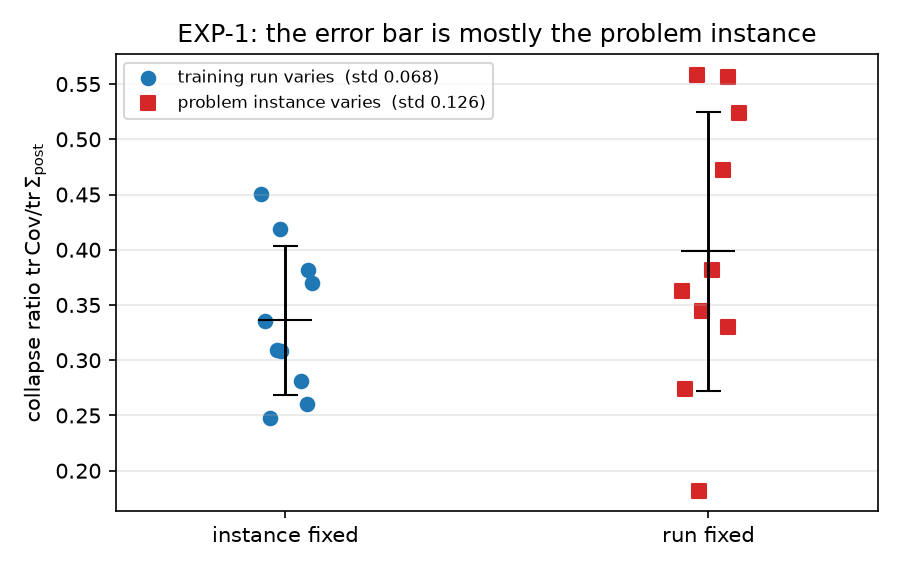
\includegraphics[width=\textwidth]{fig_seed_split.png}
\caption{What the EXP-1 error bars are measuring. \textbf{(a)} ten runs with the
problem instance held fixed and the training run varying, against ten with the
reverse; the shaded blocks are the min--max spans, and the circled point is the one
run both arms share. \textbf{(b)} the two standard deviations and their quadrature
sum against the published five-seed spread: the two sources account for the observed
bar, so nothing else of comparable size is missing from the decomposition.
\textbf{(c)} the bars next to the effect they are attached to. The collapse is
$0.63$ in ratio units and the widest bar is $0.14$, so the bars being conservative
changes their width and not a single conclusion.}
\label{fig:seedsplit}
\end{figure}

In Table~\ref{tab:seedsplit} and Figure~\ref{fig:seedsplit}, the problem
instance carries
$0.1261^2/(0.1261^2+0.0675^2)=78\%$ of the variance and the
training run $22\%$. So roughly three quarters of every EXP-1 error bar in this paper is
which operator $A$ happened to be drawn, not how the run went; genuine run-to-run
variability is about half of what the published bars imply. This does not change any
conclusion---the collapse effects are far larger than either component---but it means
the bars are conservative as measures of reproducibility, and that fixing the instance
would tighten every interval in Table~\ref{tab:sweeps} without a single additional run.
We report it rather than retrofitting it into the existing tables, whose numbers were
produced under the conflated protocol.

\subsection{An $N$-sweep on EXP-3, and what it actually measures (empirical)}
\label{sec:nsweep3}

Table~\ref{tab:sweeps} sweeps $N$ on EXP-1 at a fixed iteration budget. We repeat
that sweep on the image experiment, and add the control the EXP-1 version lacks.

At $N\in\{100,500,2000\}$ and a fixed $30000$ iterations with batch $64$
(3 seeds each), the inpaint-region pixel variance rises monotonically with $N$, by
$14.9\times$, with a log--log slope of $+0.90$ (Table~\ref{tab:nsweep3}A). Taken
alone that looks like a clean scaling law in $N$. It is not safe to read it that
way. At a fixed budget the number of gradient samples each training image receives
is $30000\times64/N$, i.e.\ exactly proportional to $1/N$, so ``variance grows like
$N$'' and ``variance grows as optimisation progress per image shrinks'' are the same
curve. A slope of $\approx+1$ is what \emph{either} explanation predicts.

Two controls separate them. Holding the per-image exposure fixed at $3840$ gradient
samples instead ($N{=}100$ at $6$k iterations, $N{=}500$ at $30$k, $N{=}2000$ at
$120$k), the slope drops to $-0.29$ and the spread from $14.9\times$ to
$2.3\times$; $N{=}500$ and $N{=}2000$ then differ by $3\%$, against a $17\%$
seed-to-seed standard deviation (Table~\ref{tab:nsweep3}B, Figure~\ref{fig:nsweep3}).
Lining the runs up by training loss instead of by iteration---a control that does not
assume exposure is the right currency---gives the same answer: $N{=}500$ and
$N{=}2000$ agree to $6$--$13\%$ with inconsistent sign at every loss level, while
$N{=}100$ sits about $2\times$ lower (Table~\ref{tab:nsweep3}C).

So most of the apparent $N$-dependence at fixed budget is an optimisation-budget
effect, and the residual genuine effect is a factor $\approx2$ rather than
$\approx15$. This is what Proposition~\ref{prop:collapse} would lead one to expect:
the population minimiser is collapsed for \emph{every} finite $N$, so a large
intrinsic $N$-dependence would be the surprising outcome. It also sharpens the
caveat already attached to the EXP-1 sweep in Table~\ref{tab:sweeps}, which shares
the same fixed-budget design and therefore the same confound: that sweep is best
read as a statement about how far a fixed budget gets you at each $N$, not about
how the population optimum depends on $N$. Appendix~\ref{sec:p6exposure} reruns the
EXP-1 sweep under exactly this control and finds the same thing there
($20.2\times\to2.28\times$), on a different architecture, dimension and dataset.

\begin{table}[htb]
\centering\small
\begin{tabular}{lccc}
\toprule
\textbf{A. constant budget} ($30000$ iters, 3 seeds) & $N{=}100$ & $N{=}500$ & $N{=}2000$\\
\midrule
grad.\ samples per image & $19200$ & $3840$ & $960$\\
inpaint pixel variance   & $1.20(21)\times10^{-4}$ & $4.48(74)\times10^{-4}$ & $1.79(24)\times10^{-3}$\\
NN distance to train image & $7.4(2.9)\times10^{-5}$ & $3.71(5)\times10^{-4}$ & $1.30(31)\times10^{-3}$\\
\midrule
\textbf{B. constant exposure} ($3840$/image, seed 0) & $N{=}100$ & $N{=}500$ & $N{=}2000$\\
\midrule
iterations               & $6000$ & $30000$ & $120000$\\
inpaint pixel variance   & $8.59\times10^{-4}$ & $3.79\times10^{-4}$ & $3.68\times10^{-4}$\\
final training loss      & $0.0159$ & $0.0089$ & $0.0080$\\
\midrule
\textbf{C. matched training loss} & $N{=}100$ & $N{=}500$ & $N{=}2000$\\
\midrule
at loss $0.020$          & $1.09\times10^{-3}$ & $2.77\times10^{-3}$ & $3.13\times10^{-3}$\\
at loss $0.015$          & $7.76\times10^{-4}$ & $1.23\times10^{-3}$ & $1.37\times10^{-3}$\\
at loss $0.010$          & $3.15\times10^{-4}$ & $6.16\times10^{-4}$ & $5.80\times10^{-4}$\\
\bottomrule
\end{tabular}
\caption{EXP-3 $N$-sweep (empirical, not determined by the population theory).
Panel A is the fixed-budget sweep: slope $+0.90$ in $\log N$, spread $14.9\times$.
Panel B holds the per-image gradient exposure fixed instead: slope $-0.29$, spread
$2.3\times$. Panel C lines the runs up by training loss, interpolating over every
checkpoint of every run at that $N$. Parenthesised digits are the standard deviation
over 3 seeds in the last digits shown; panels B and C use a single seed per point,
so the $N{=}100$ gap in B (whose run is also the least converged, loss $0.0159$) is
best read together with C rather than alone.}
\label{tab:nsweep3}
\end{table}

\begin{figure}[htb]
\centering
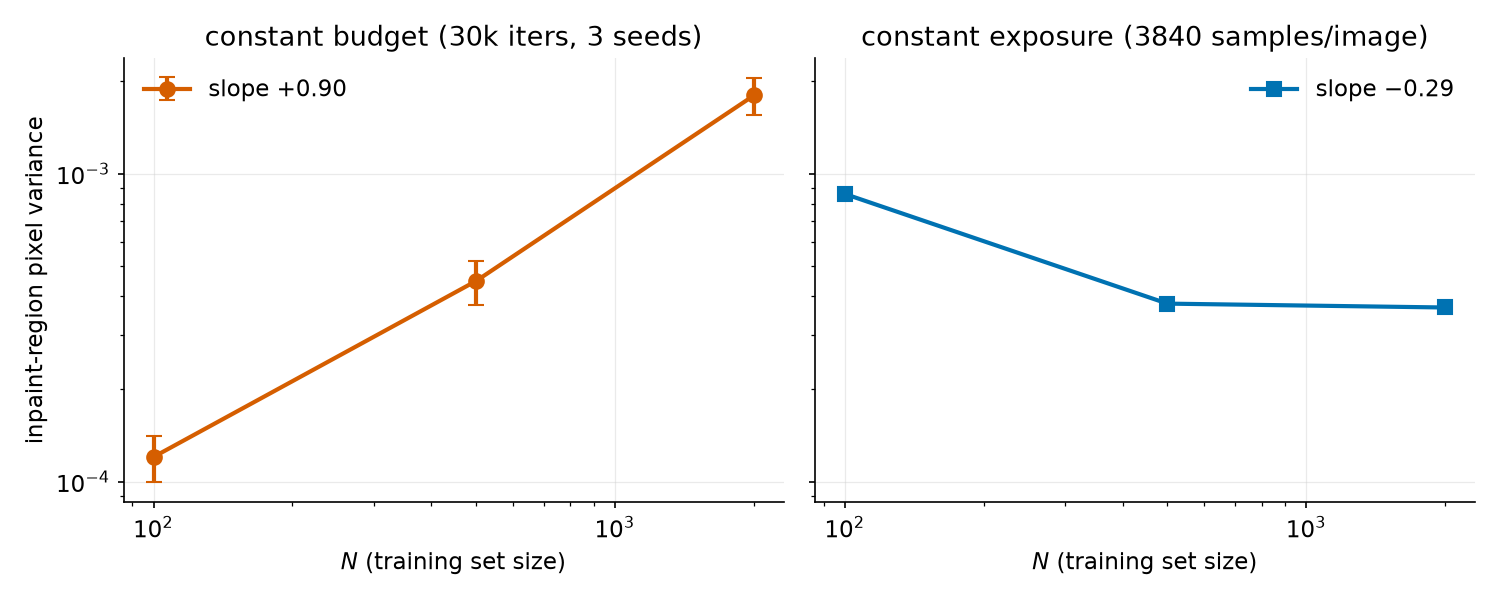
\includegraphics[width=0.85\textwidth]{fig_exp3_n_sweep.png}
\caption{EXP-3 $N$-sweep on a shared $y$-axis. Left: at a fixed $30000$-iteration
budget the inpaint-region variance rises like $N^{+0.90}$. Right: at a fixed
per-image gradient exposure the same three $N$ values are nearly flat. The
difference between the panels is the confound, not the data.}
\label{fig:nsweep3}
\end{figure}

\subsection{Additional verification (gap to optimum, Lipschitz, posterior distance)}
\label{sec:aux}

\paragraph{The bandwidth expansion, measured.} Proposition~\ref{prop:expansion} is the
one result here about a \emph{random} design, and on the linear-Gaussian instance it can
be checked without training anything: draw datasets, compute $\tr\Covh(y)$, compare.
Figure~\ref{fig:expansion} does that at $N{=}2000$ over $24$ draws per bandwidth. Three
things are visible. The exact population law for this instance---$\tr\Sigmapost
+\|J\|_F^2\,h^2\Sigma_Y/(\Sigma_Y+h^2)$, which follows from the $h$-tilted law of a
Gaussian design being Gaussian---tracks the measurement to within $2.5\%$ wherever
$Nh^k\ge100$. The proposition's $h^2\|J\|_F^2$ is the small-$h$ limit of that law and
departs from it by $7.7\%$ at $h{=}1$, which is the $O(h^4)$ term the statement
discards, becoming visible. And the spread across draws falls as $(Nh^k)^{-1/2}$: fitted
$-0.48$ against the predicted $-0.5$ over three decades of $Nh^k$, which is the
$O_P((Nh^k)^{-1/2})$ term of the statement measured rather than assumed. Below
$Nh^k\approx100$ the measurement sits \emph{under} the law by up to $6\%$, the plug-in
covariance's own $1/n_{\mathrm{eff}}$ bias ($n_{\mathrm{eff}}\approx37$ at $h{=}0.02$):
the regime where the expansion's error term dominates its signal.

\begin{figure}[htb]
\centering
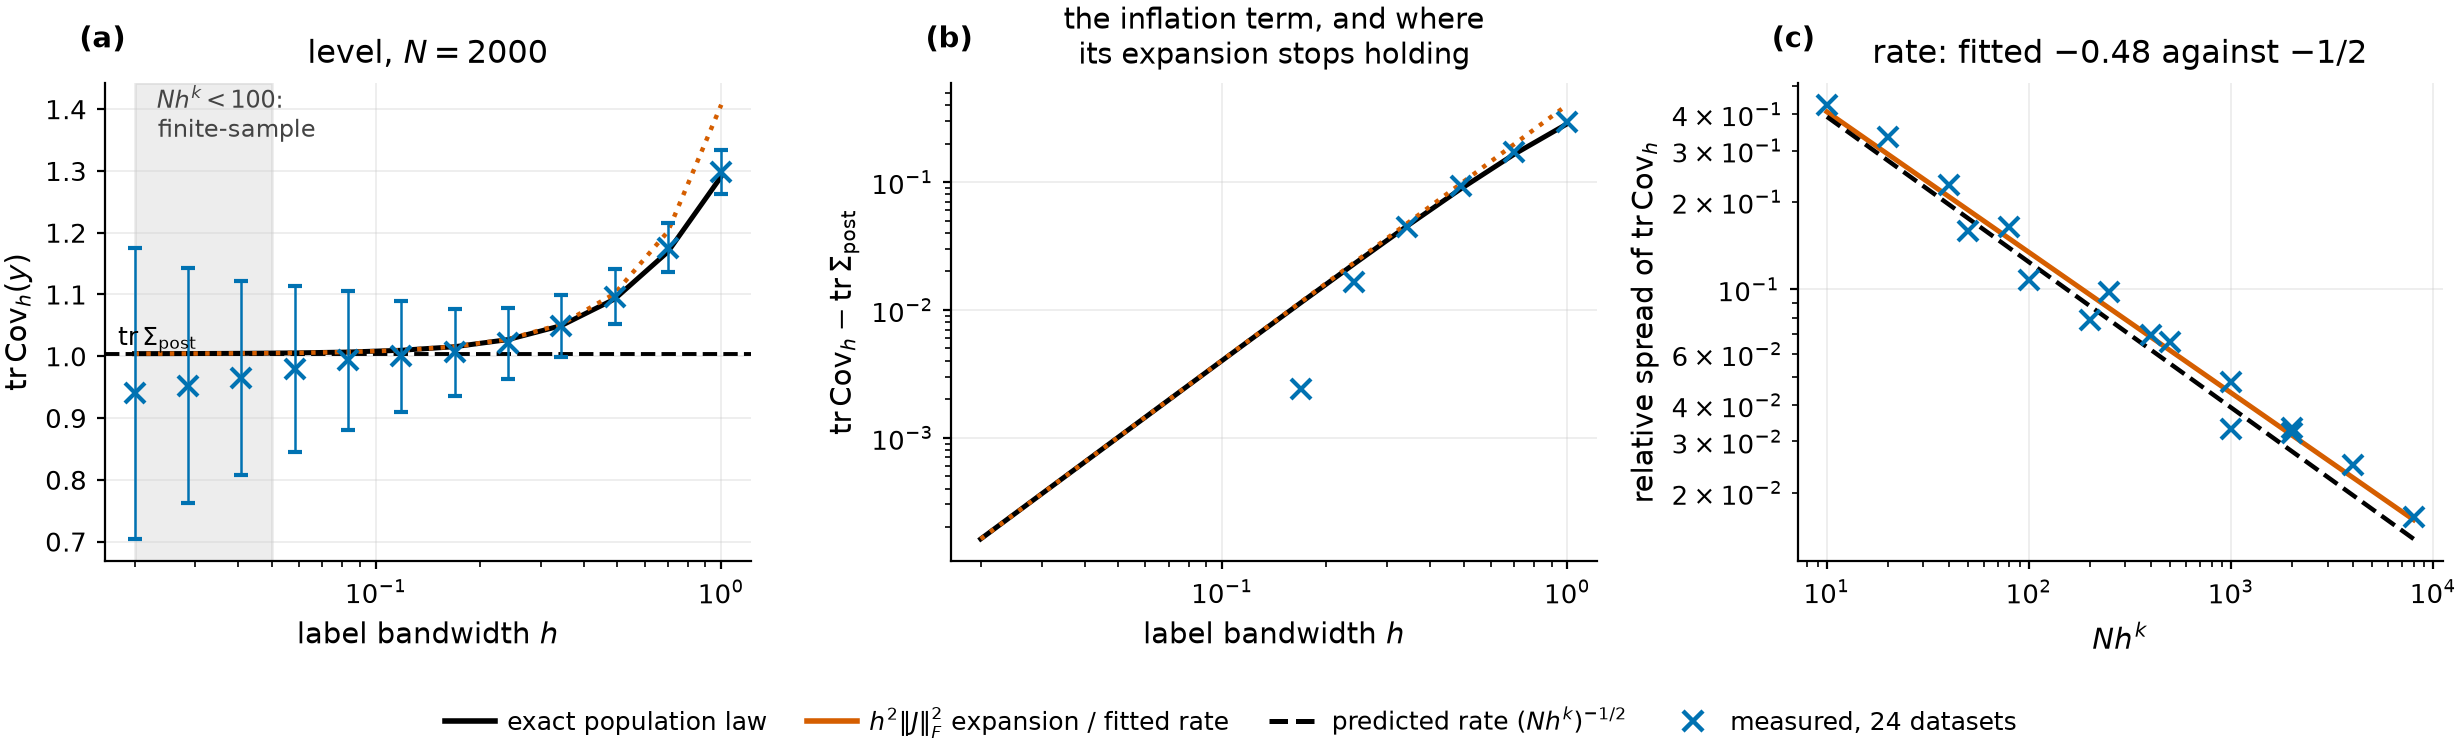
\includegraphics[width=\textwidth]{fig_expansion.png}
\caption{Proposition~\ref{prop:expansion} against measurement on the linear-Gaussian
instance ($N{=}2000$, $24$ datasets per bandwidth, error bars one standard deviation
across draws). (a) the level: the exact population law (solid) and its small-$h$
expansion $\tr\Sigmapost+h^2\|J\|_F^2$ (dotted) against the measured trace; the shaded
band is $Nh^k<100$, where the $O_P$ term dominates. (b) the inflation term alone, on
log axes, where the two curves separate above $h\approx0.5$; bandwidths whose measured
excess is negative (the finite-sample bias, panel (a)) cannot be drawn on a log axis and
are omitted. (c) the rate: the relative spread across draws against $Nh^k$, fitted
$-0.48$ against the predicted $-1/2$. Produced by
\texttt{scripts/make\_expansion\_figure.py}, which asserts each of these before
drawing.}
\label{fig:expansion}
\end{figure}

Three checkpoint-only measurements corroborate the theory.
(i)~\emph{Optimality gap.} The Monte-Carlo gap $L(v_\theta)-L(\vstar)$, with
$L(\vstar)=\E[\Var(U\mid X_t,t,\widetilde Y)]$ computed from the exact minimiser, is
non-negative at every checkpoint and decreases monotonically toward $0$ at every $h$
(e.g.\ $h{=}0.1$: $1.14\to0.22\to0.102$ at $10^2/3{\times}10^4/2{\times}10^5$ steps),
consistent with ratio-to-kernel $\to1$. The irreducible error $L(\vstar)$ increases
with $h$ ($0\to1.88$): the price of smoothing (Figure~\ref{fig:optgap}).

\begin{figure}[htb]
\centering
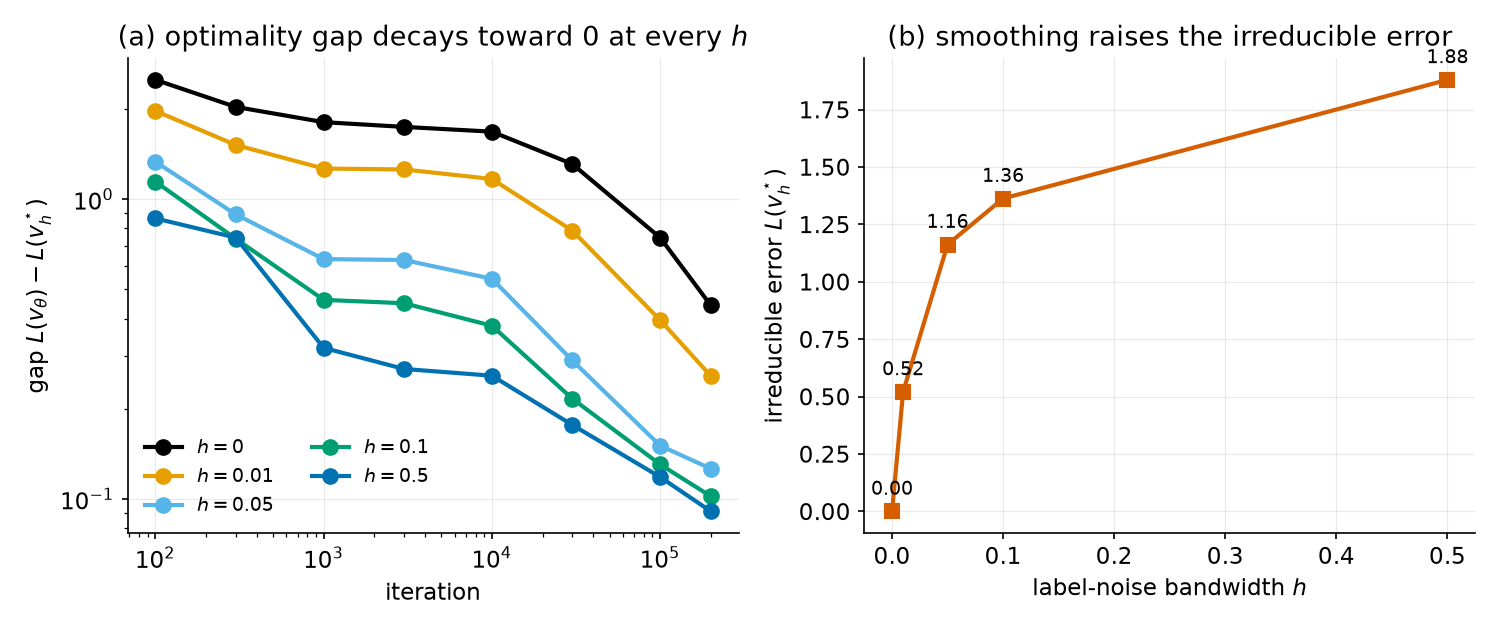
\includegraphics[width=0.85\textwidth]{fig_optgap.png}
\caption{Optimality gap $L(v_\theta)-L(v_h^\star)$ decays monotonically \emph{toward}
$0$ at every $h$ (left)---it is still positive at the last checkpoint
($0.09$--$0.44$), which is the optimisation gap of
Section~\ref{sec:limitations}; smoothing raises the irreducible error
$L(v_h^\star)$ (right).}
\label{fig:optgap}
\end{figure}

(ii)~\emph{Lipschitz floor.} The empirical $\operatorname{Lip}_x v_\theta$ grows from
$7.1$ at $t{=}0.5$ to $65.7$ at $t{=}0.99$; the Corollary~\ref{cor:floor} floor
$d/(3L)\approx0.010$ is $\sim50\times$ below the observed plateau $0.48$, so this
particular representation-capacity argument does \emph{not} explain the plateau: the
measured plateau is inconsistent with the Lipschitz-floor explanation tested here (we
have ruled out \emph{this} mechanism, not every possible capacity/representation
effect) and, as the learning-rate-schedule result of Section~\ref{sec:exp1} shows, is
strongly schedule-sensitive---suggesting an optimisation rather than a Lipschitz-capacity
limitation, though we do not have a positive quantitative theory of the optimisation
gap itself (Section~\ref{sec:limitations}) (Figure~\ref{fig:lipschitz}).

\begin{figure}[htb]
\centering
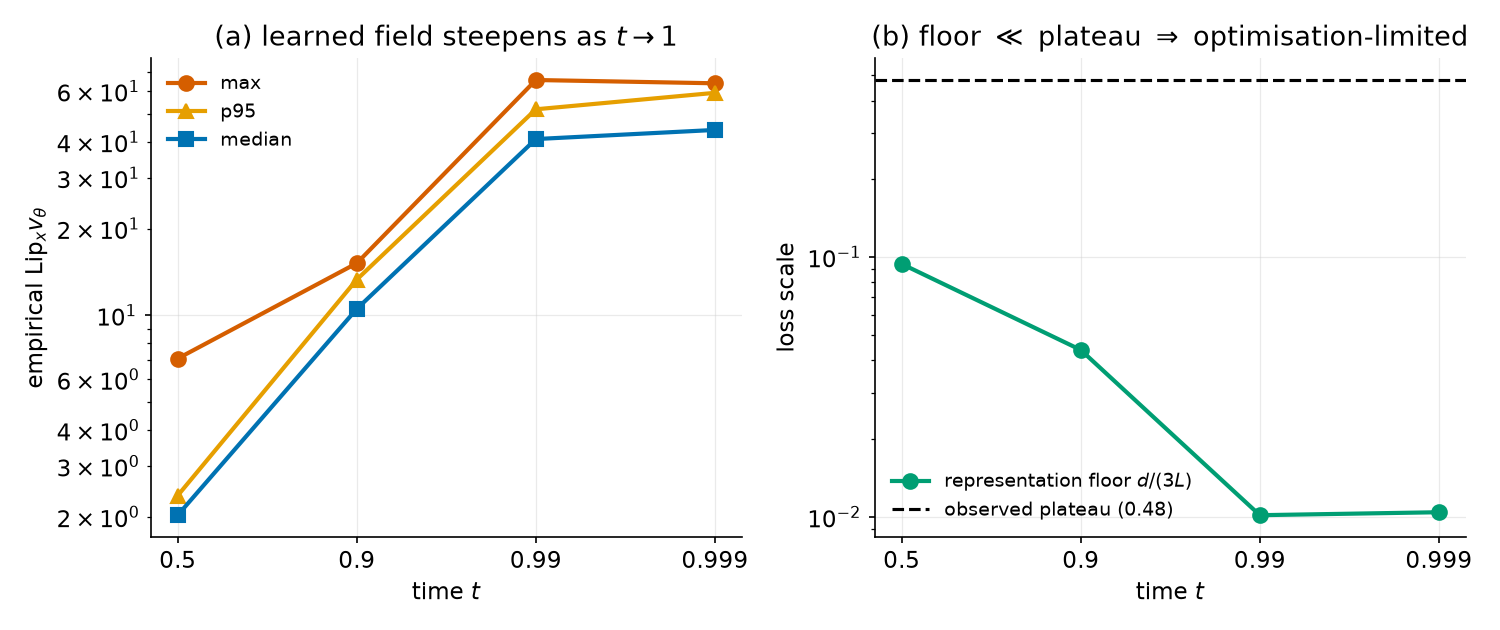
\includegraphics[width=0.85\textwidth]{fig_lipschitz.png}
\caption{The empirical Lipschitz constant of $v_\theta$ blows up as $t\to1$ (left); the
representation floor $d/(3L)$ is $\sim50\times$ below the observed loss plateau (right),
ruling out this particular Lipschitz-capacity explanation and pointing toward an
optimisation-limited plateau instead.}
\label{fig:lipschitz}
\end{figure}

(iii)~\emph{Posterior distance.} Both distances to the analytic posterior
$\N(\mu_{\mathrm{post}},\Sigmapost)$ fall monotonically with $h$---MMD
$0.256\to0.012$, entropic OT $1.34\to0.119$---and neither approaches zero
(Figure~\ref{fig:postdist}). Zero, however, is the wrong thing to compare against: no
finite sample reaches it, so we compute the two scales that make the numbers readable,
both from ground truth alone and both free of any trained model
(\texttt{scripts/analyze\_posterior\_reference\_scales.py}). The \emph{sampling floor}
is what the same estimators return for two independent $M{=}1000$ draws from the
\emph{same} posterior: ${\rm MMD}=0.00073$, $\sqrt{S_\varepsilon}=0.075$. The
\emph{atomic prediction} is the distance from the posterior to
$\sum_ip_i^{(h)}\delta_{x^i}$, the law Theorem~\ref{thm:endpoint} says the model
converges to. The measured curves track that prediction closely at every
$h\ge0.05$---at $h{=}0.5$, $\sqrt{S_\varepsilon}=0.345$ measured against $0.333$
predicted---and the prediction itself stops $4.6\times$ above the sampling floor in
$W_2$ and $14\times$ above it in MMD. In the data's own units the best bandwidth
leaves the generated law $0.345$ from the posterior, which is $34\%$ of the posterior's
own width $\sqrt{\tr\Sigmapost}=1.00$.

An earlier version of this paper read the OT curve's apparent plateau as a numerical
witness of the floor \eqref{eq:w2floor}. That reading was wrong twice over. The
numbers were produced by the Sinkhorn implementation corrected in
Section~\ref{sec:p7}, so the plateau was an artefact; and the floor is in any case
directly computable, equals $0.0353$ here---$3.5\%$ of $\tr\Sigmapost$---while the
population-optimal atomic law already reaches ${\rm MMD}=0.0089$, below what the
trained model attains. What the corrected curves do show is the claim the paper makes:
the model converges to the atomic law the theory names, and that law does not converge
to the posterior. Atomicity is real (Proposition~\ref{prop:atomicity} is exact); what
these curves measure is the model arriving at it.

\begin{figure}[htb]
\centering
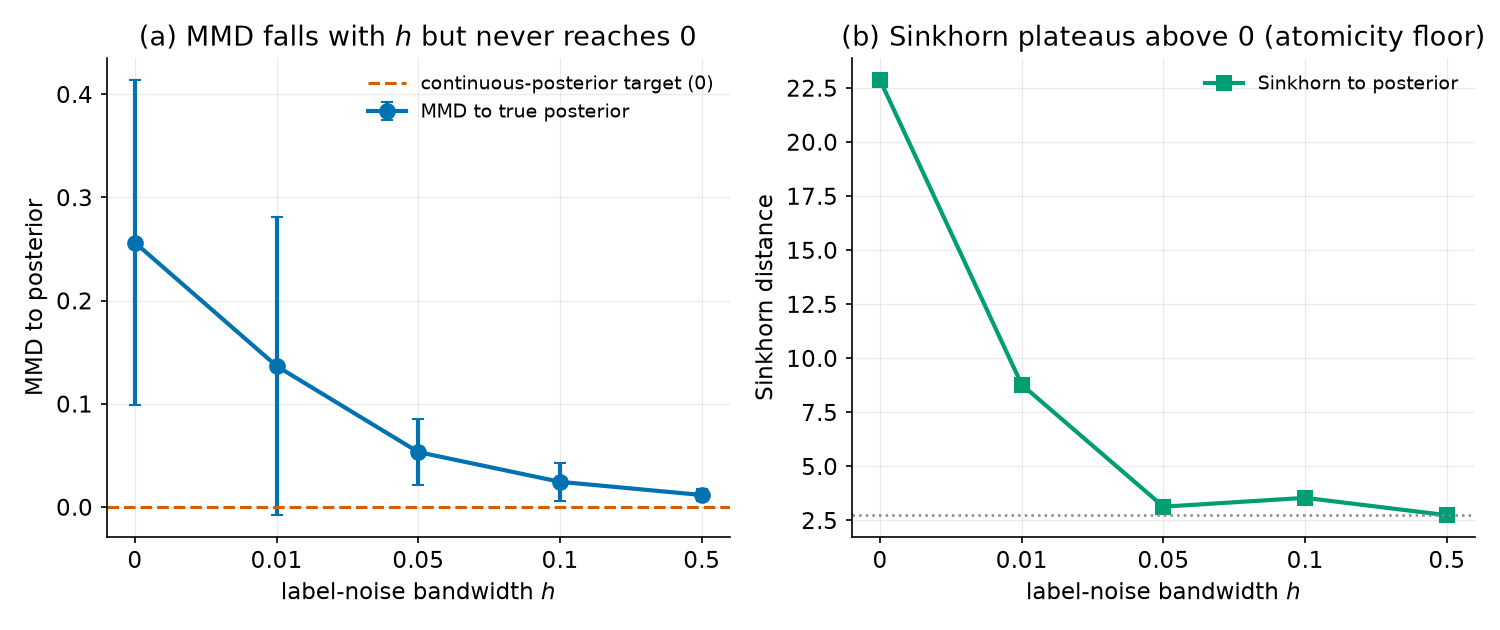
\includegraphics[width=\textwidth]{fig_posterior_distance.png}
\caption{Distance to the true posterior, against the two scales that make it
readable. \textbf{(a)} MMD. The \emph{sampling floor} (green) is what the same
estimator returns for two independent $M{=}1000$ draws from the same posterior---the
bottom of the axis in practice, since $0$ is not reachable at finite $M$. The
\emph{atomic prediction} (orange) is the distance to $\sum_ip_i^{(h)}\delta_{x^i}$,
the law Theorem~\ref{thm:endpoint} names; it is where the theory puts the model, not
an artefact of the estimator. The measured curve falls onto it and the pair stop
$14\times$ above the floor. \textbf{(b)} the same in $W_2$ units, so the numbers are
lengths in the data's own scale: at the best bandwidth the law sits $0.345$ from a
posterior $1.00$ wide, $4.6\times$ the floor. \textbf{(c)} why: $n_{\mathrm{eff}}$,
the number of training atoms the mixture actually uses, is at most $66$ of $200$---the
law is a finite mixture of point masses at every $h$, which is
Proposition~\ref{prop:atomicity}. Panel (c) is over the eight conditions of this
sweep, all from seed $0$, so that it describes the same measurements as (a) and (b);
the five-seed averages quoted in Section~\ref{sec:p7} ($26$ and $102$) are larger and
make the same point with more of the label space. Raising $h$ moves the model towards the posterior;
the thing it moves towards is atomic.}
\label{fig:postdist}
\end{figure}

(iv)~\emph{Does the gap close with budget?} Items (i)--(iii) leave open whether the
residual gap at $h>0$ is an optimisation gap that a longer run would close, or a
representation floor that no budget can. We test this directly by extending the
$h{=}0.1$ run to $10^6$ iterations under the cosine schedule of
Section~\ref{sec:exp1}, over 5 seeds (Table~\ref{tab:gaph01},
Figure~\ref{fig:gaph01}). The covariance reaches the kernel optimum early and stays
there ($\tr\Cov/\tr\Covh = 1.65 \to 1.00$ by $10^5$, then flat to $10^6$), while the
mean error $\|\text{mean}-\bar x_h\|$ keeps falling, $0.188 \to 0.0534$ at $10^5$
$\to 0.0220$ at $10^6$: a further factor $2.4$ over the last decade of budget, with
no sign of a floor. A representation limit would show as a plateau; none appears
within $10^6$ iterations. This is positive evidence for the optimisation-paced
reading of Section~\ref{sec:limitations}, complementing the elimination argument in
(ii)---though it bounds the gap from one side only, and does not tell us where the
floor eventually lies.

Read this against the \emph{wrong} lens for comparison. The relative velocity error
to the collapsed field $(x^{i}-x)/(1-t)$ of Section~\ref{sec:theory-hard} barely moves at $h{=}0.1$
($0.78\to0.65$ over the same $10^6$ iterations) while at $h{=}0$ it falls
$0.78\to0.15$. That is not a representation limit either: the reference $\vstar$ at
$h{=}0$ does not depend on $h$, so at $h{=}0.1$ a model that correctly refuses to
collapse \emph{must} stay far from it. The $h$-aware Proposition~\ref{prop:moments}
quantities are the only ones that answer the question, which is why they are what
Table~\ref{tab:gaph01} reports.

\begin{table}[htb]
\centering\small
\begin{tabular}{lccccc}
\toprule
iteration & $10^2$ & $10^4$ & $10^5$ & $4\times10^5$ & $10^6$\\
\midrule
$\tr\Cov/\tr\Covh$        & $1.649$ & $1.062$ & $1.002$ & $0.997$ & $1.004$\\
$\|\text{mean}-\bar x_h\|$ & $0.188$ & $0.151$ & $0.0534$ & $0.0314$ & $0.0220$\\
$\tr\Cov$                  & $1.091$ & $1.087$ & $1.035$ & $1.018$ & $1.056$\\
\bottomrule
\end{tabular}
\caption{EXP-1 at $h{=}0.1$, extended to $10^6$ iterations (median over 5 seeds;
$\tr\Sigmapost=1.004$). The covariance matches the kernel optimum from $10^5$ on;
the mean error is still decreasing at the end of the budget. At $h{=}0$ under the
same schedule and seeds, $\tr\Cov$ instead falls $1.087\to0.115$ and $n_{\rm eff}=1$
throughout---full collapse---whereas here $n_{\rm eff}=25.1$ (median; $13.7$--$43.9$
across seeds) and is a property of $(X,Y,h)$ alone, not of training. The two small
increases in the mean-error row ($10^5\!\to\!2{\times}10^5$ and
$4\!\times\!10^5\!\to\!7{\times}10^5$, not shown) are within seed noise. Per seed at
$10^6$ the mean error is $0.019$--$0.026$; the ratio is $0.99$--$1.03$ for four seeds
and $2.85$ for seed~4, whose draw of $A$ gives a near-degenerate $\Covh$ and so an
ill-conditioned ratio---the mean error, which does not divide by a small number, is
well behaved on that seed too.}
\label{tab:gaph01}
\end{table}

\begin{figure}[htb]
\centering
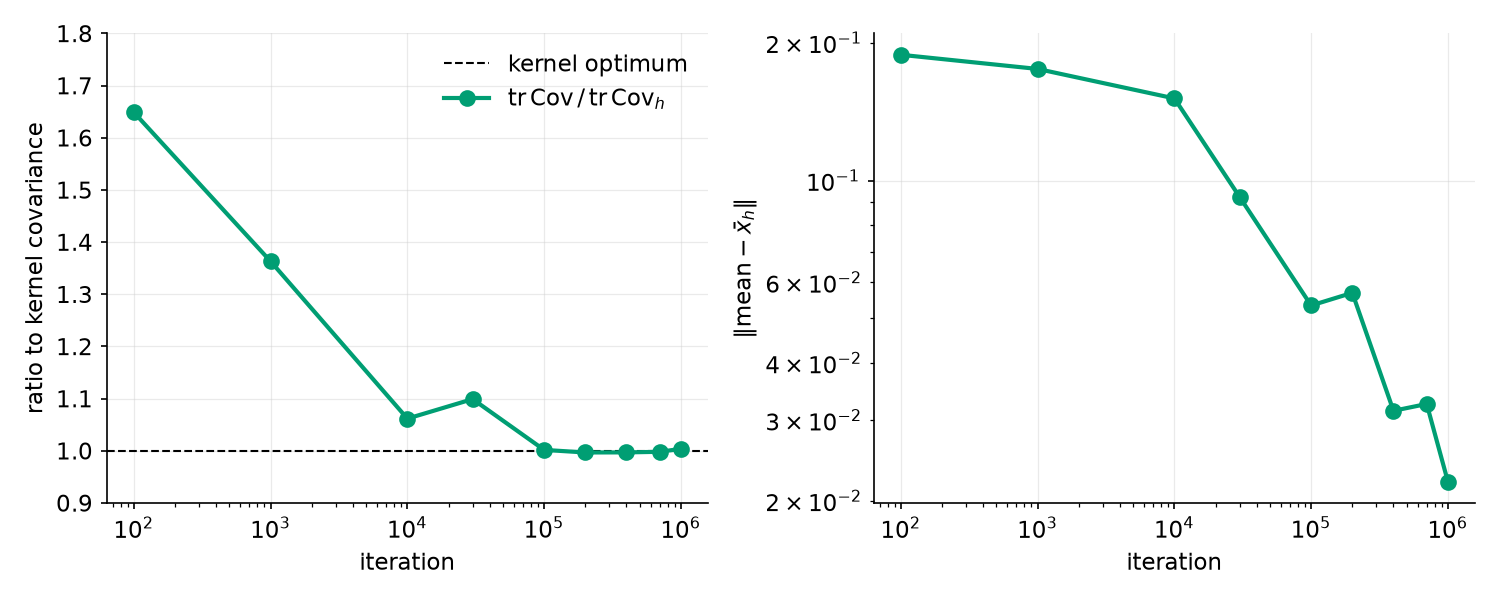
\includegraphics[width=0.85\textwidth]{fig_gap_diagnostic_h01.png}
\caption{EXP-1 at $h{=}0.1$ over $10^6$ iterations (median of 5 seeds). Left: the
covariance ratio to the Proposition~\ref{prop:moments} optimum settles at $1$ by
$10^5$. Right: the distance from the generated mean to $\bar x_h$ keeps decreasing
to the end of the budget---no representation floor is visible.}
\label{fig:gaph01}
\end{figure}

\subsection{Supporting figures and tables}
\label{app:figs}

\begin{figure}[htb]
\centering
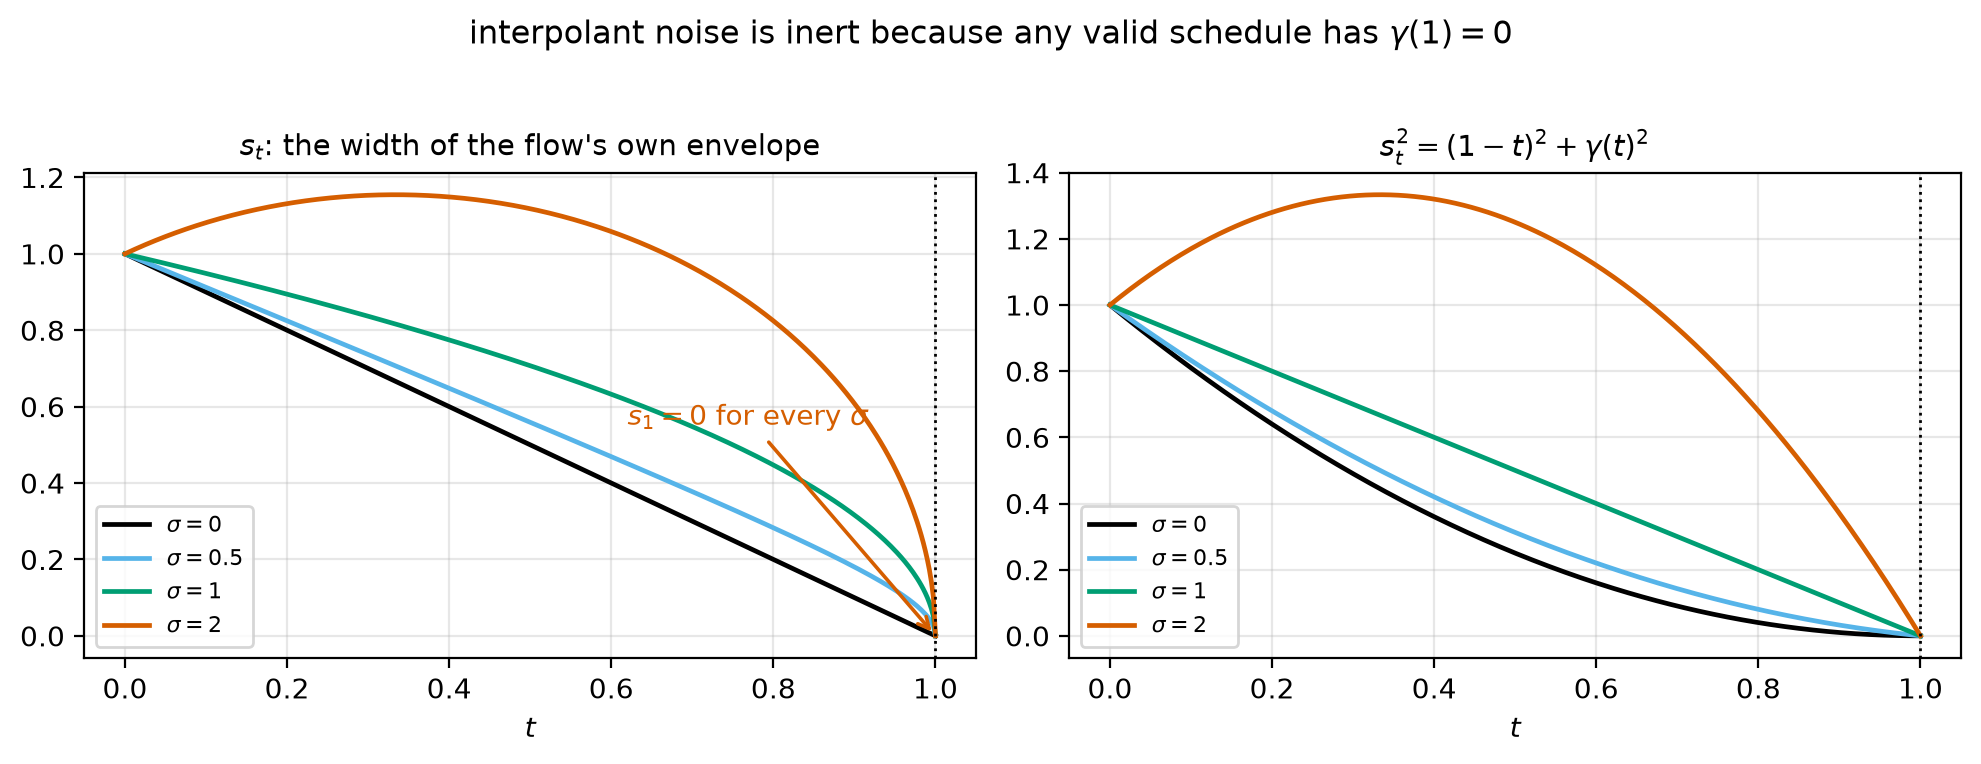
\includegraphics[width=0.74\textwidth]{fig_interpolant.png}
\caption{Why Proposition~\ref{prop:prop17} is structural rather than accidental. The
flow is $x_t=t\,x^i+s_t\,x_0$ with $s_t^2=(1-t)^2+\gamma(t)^2$, so the endpoint is
decided entirely by $s_1$. Interpolant noise widens the envelope in the middle of the
interval---visibly so, and more for larger $\sigma$---but every schedule that is a
valid interpolant must satisfy $\gamma(1)=0$, since otherwise the path never reaches
the data. The envelope is therefore pinned to zero at $t=1$ for every $\sigma$, and
the endpoint law is unchanged. The property that makes the noise admissible is the
property that makes it inert.}
\label{fig:interpolant}
\end{figure}

\begin{figure}[htb]
\centering
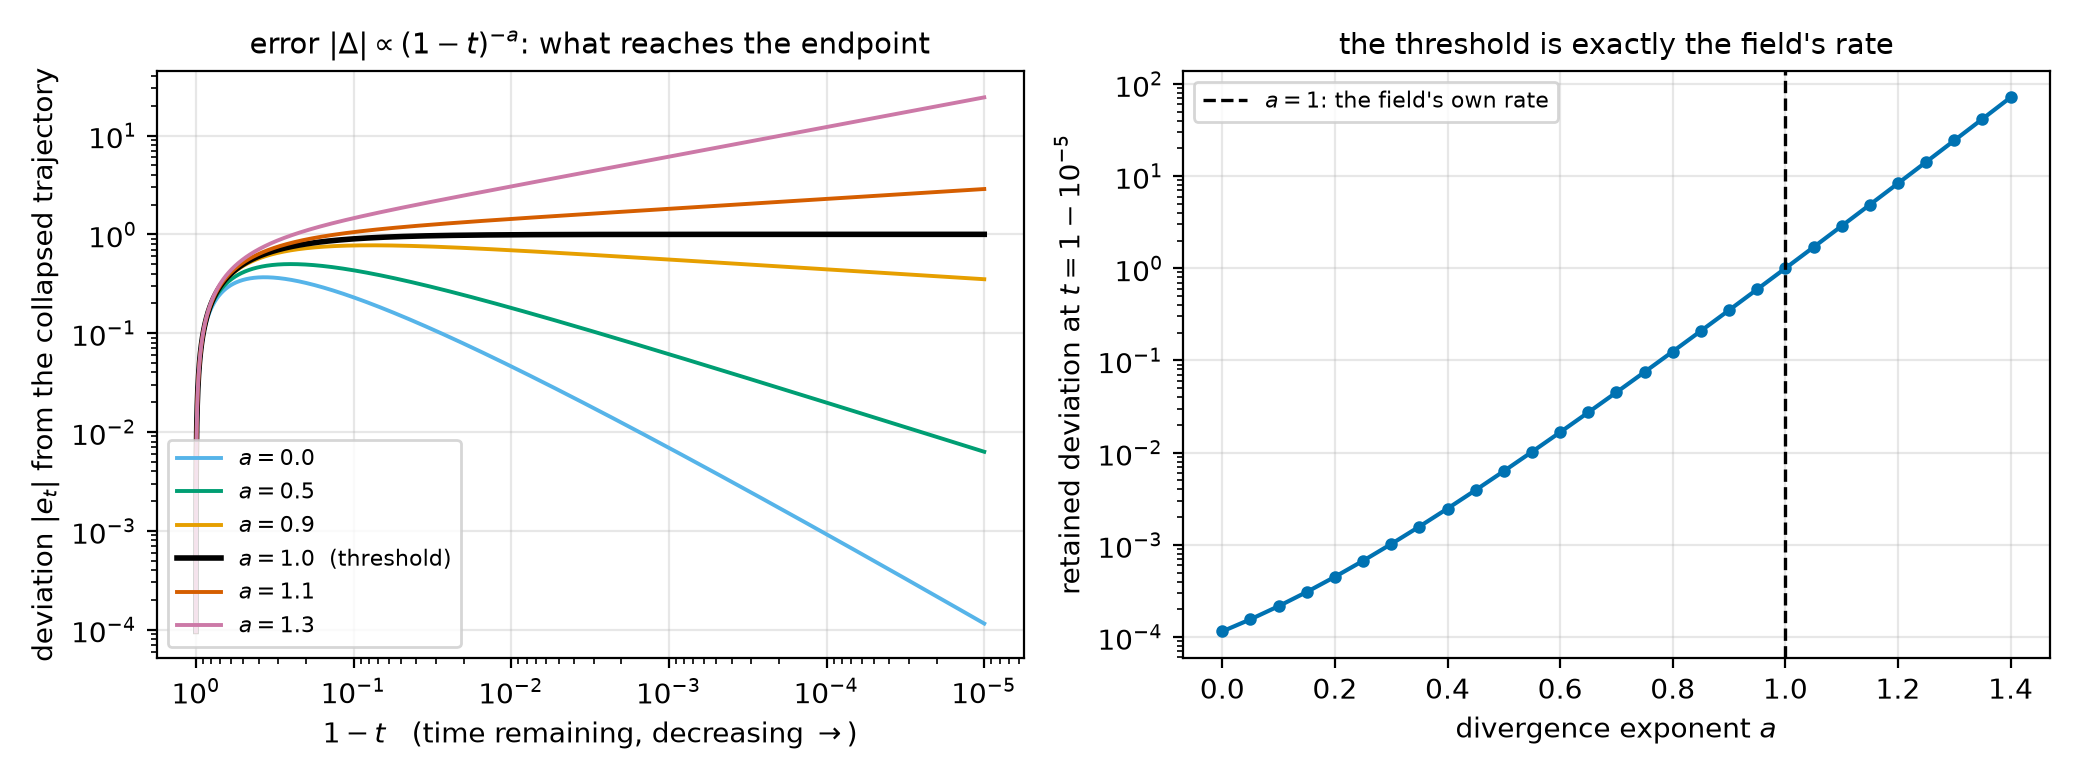
\includegraphics[width=\textwidth]{fig_survival.png}
\caption{Proposition~\ref{prop:survival} and Corollary~\ref{cor:lossform}, drawn.
\textbf{(a)} the deviation $|e_t|$ from the collapsed trajectory for velocity errors
growing like $c(1-t)^{-a}$. The exact field's linear part is $-\tfrac{1}{1-t}I_d$, a
contraction whose strength diverges, so an error only reaches the endpoint if it
diverges at the same rate: $a<1$ is driven to zero, $a=1$ is the separatrix and
flattens at the error's own coefficient $c$, and $a>1$ grows without bound. The
curves are the closed form
$|e_t|=\tfrac{c}{a}\big((1-t)^{1-a}-(1-t)\big)$---the bound
\eqref{eq:survival} attained with equality---and the open markers are the ODE
integrated numerically at three truncations, so neither is asked for on trust.
\textbf{(b)} the threshold is a statement about the limit, so the truncation is
varied rather than fixed: the curves pivot about $a=1$, fanning to $0$ below it and
to $\infty$ above, and every truncation passes through the same point $(1,c)$.
\textbf{(c)} the loss form against what EXP-1 actually did. Equation
\eqref{eq:lossform} predicts the retained conditional standard deviation scales like
$\sqrt{\mathcal L}$ at fixed truncation; the measured slope over the six checkpoints
from $10^3$ on is $0.429$ at $R^2=0.99$, and $0.485$ over the last three, against the
predicted $\tfrac12$. The offset is the constant the bound does not pin down,
$e^{L_\Delta}\approx25$, i.e.\ the inequality holds here with $L_\Delta\ge3.2$. The
exponent is the corollary's content, and the measured exponent is consistent with the
predicted $\tfrac12$ scaling; the constant is loose. The
practical reading of all three panels is that a bounded error is annihilated by the
flow, so a model can keep conditional variance only by failing to reproduce the
blow-up---the failure Remark~\ref{lem:norepr} says a finite Lipschitz network cannot
avoid---and the rate at which it stops failing is set by the loss.}
\label{fig:survival}
\end{figure}

\begin{figure}[htb]
\centering
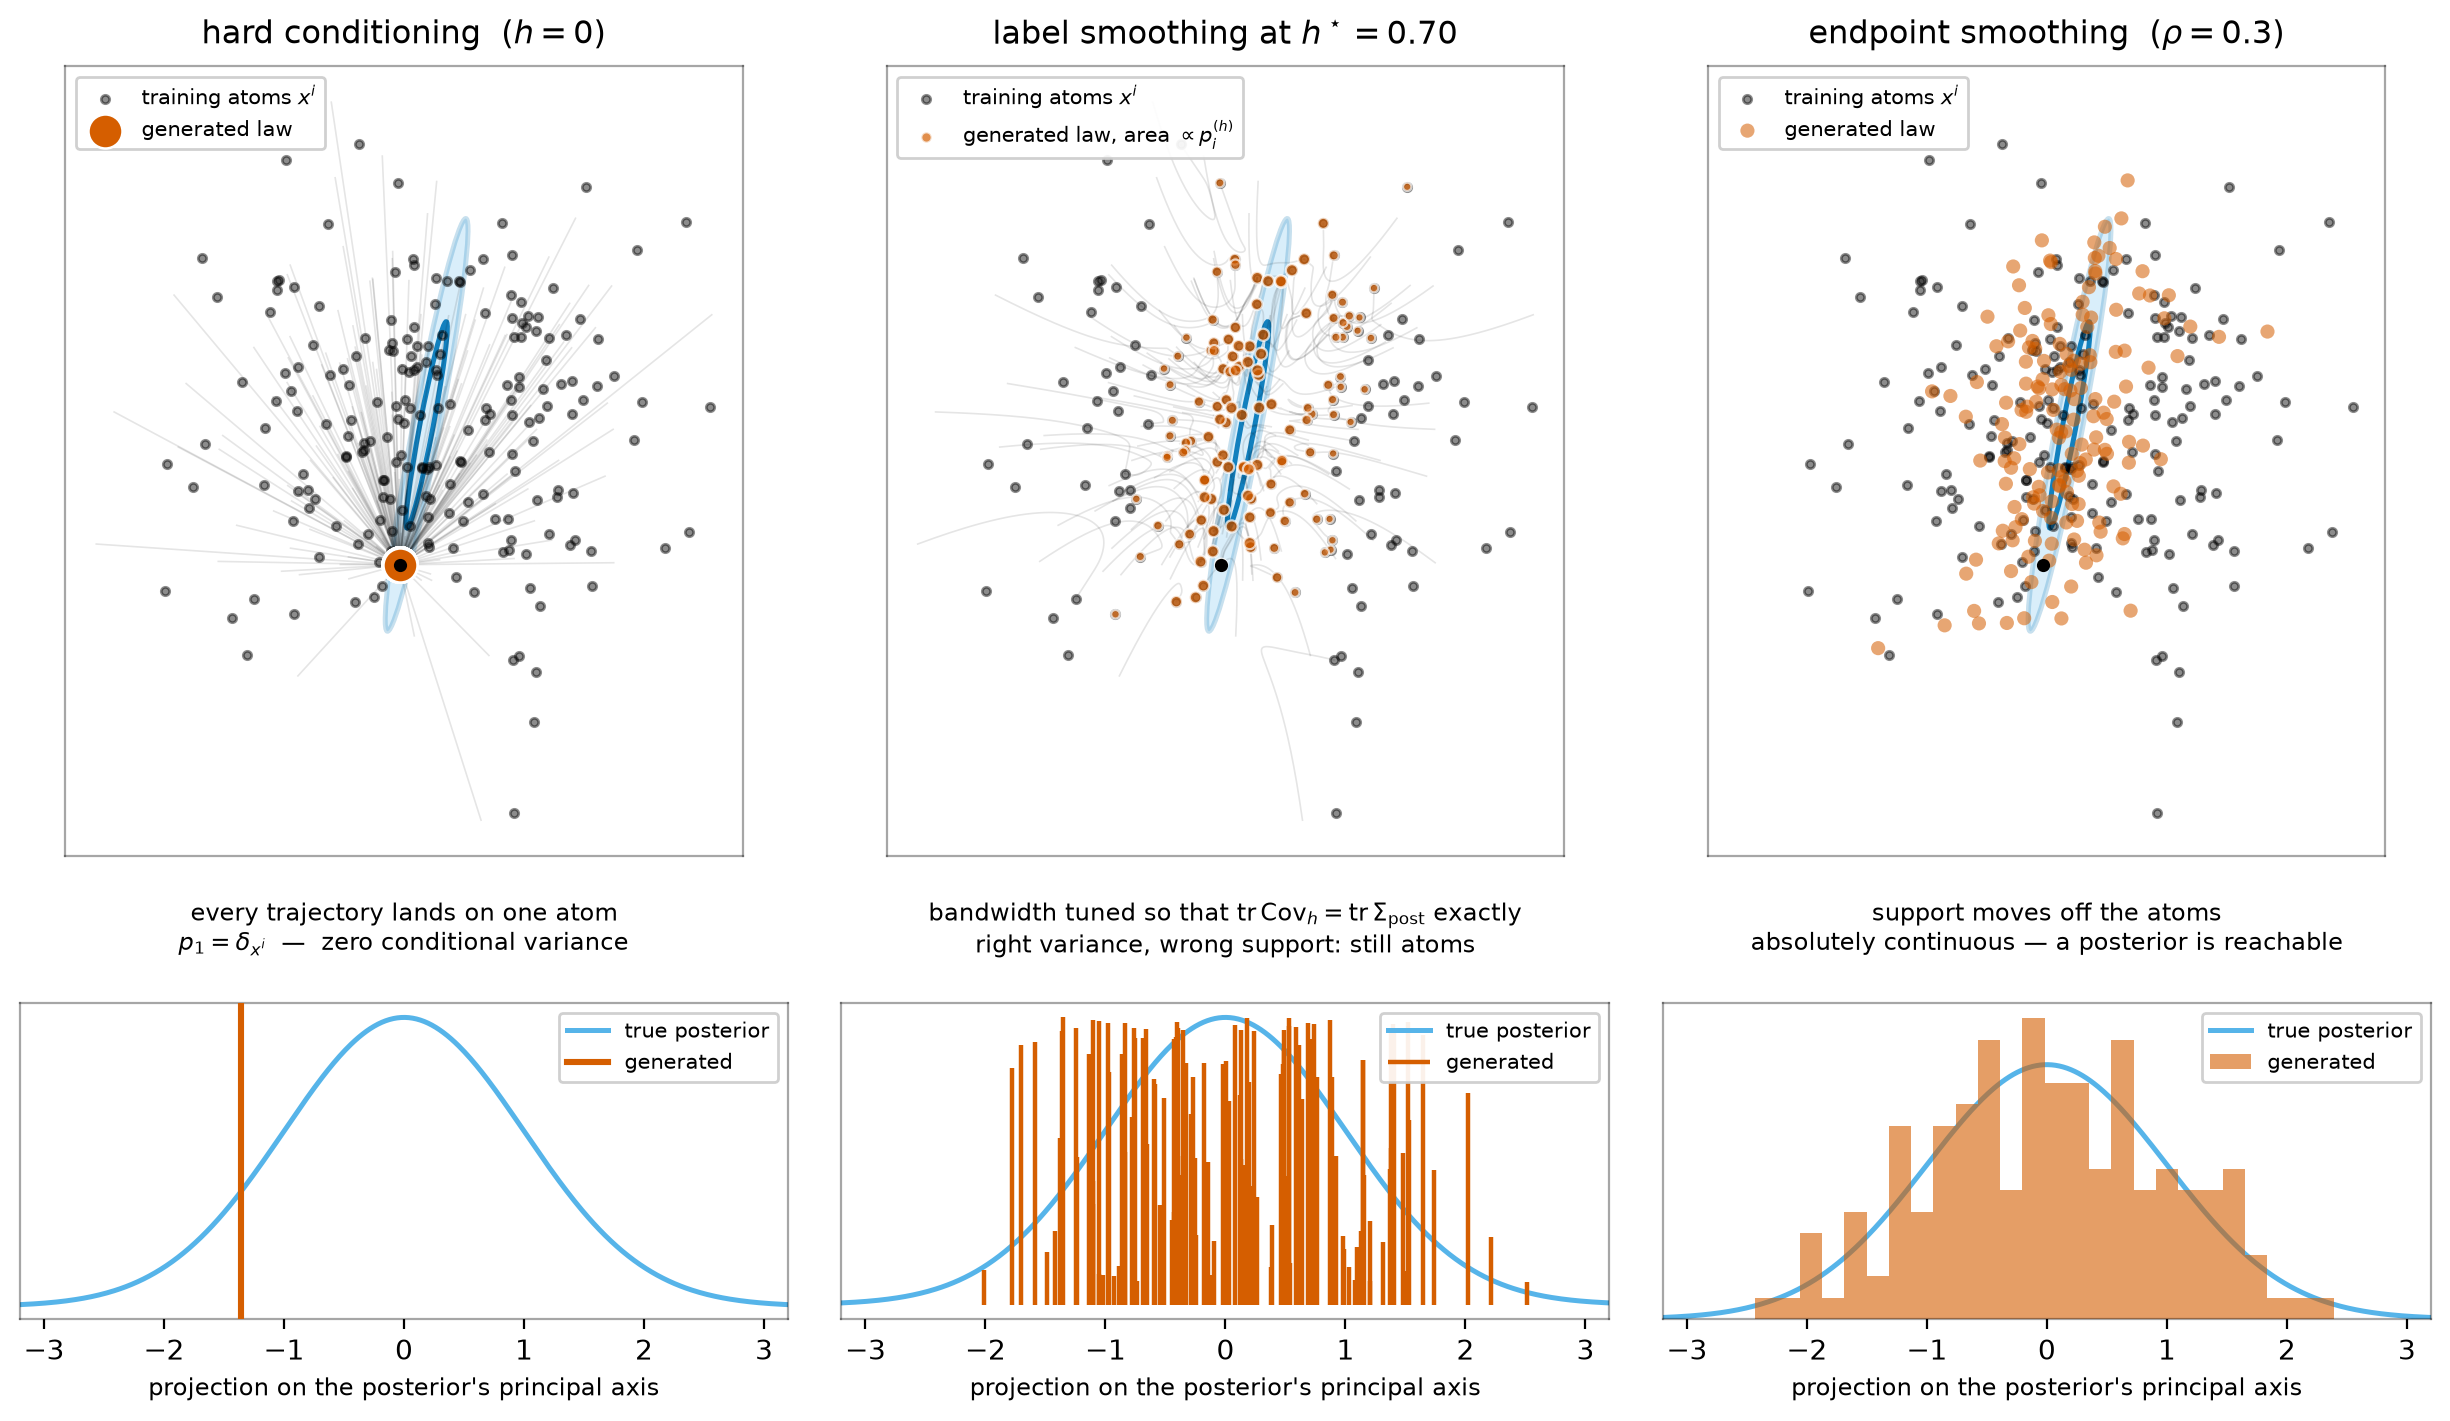
\includegraphics[width=0.94\textwidth]{fig_mechanism.png}
\caption{Figure~\ref{fig:mechanism}'s population panels with their one-dimensional
marginals, which is what the state-space view cannot show: $160$ trajectories
integrated with RK4 under each \emph{exact population} field on the real $d{=}2$
instance ($N{=}200$), the true posterior shaded, the training atoms black. The middle
panel's bandwidth is not chosen for looks---it is found by bisection so that
$\tr\Covh(y)=\tr\Sigmapost$ to four decimals ($h^\star=0.703$, $1.0040$ against
$1.0040$), so the generated law has \emph{exactly} the right conditional variance while
remaining supported on the training atoms. The
lower row projects all three laws onto the posterior's principal axis against its
density: a single spike, a forest of spikes spanning the right range, and a
continuum. Matching the second moment and matching the distribution are different
things, and the middle column is the difference.}
\label{fig:mechanismreal}
\end{figure}

\begin{figure}[htb]
\centering
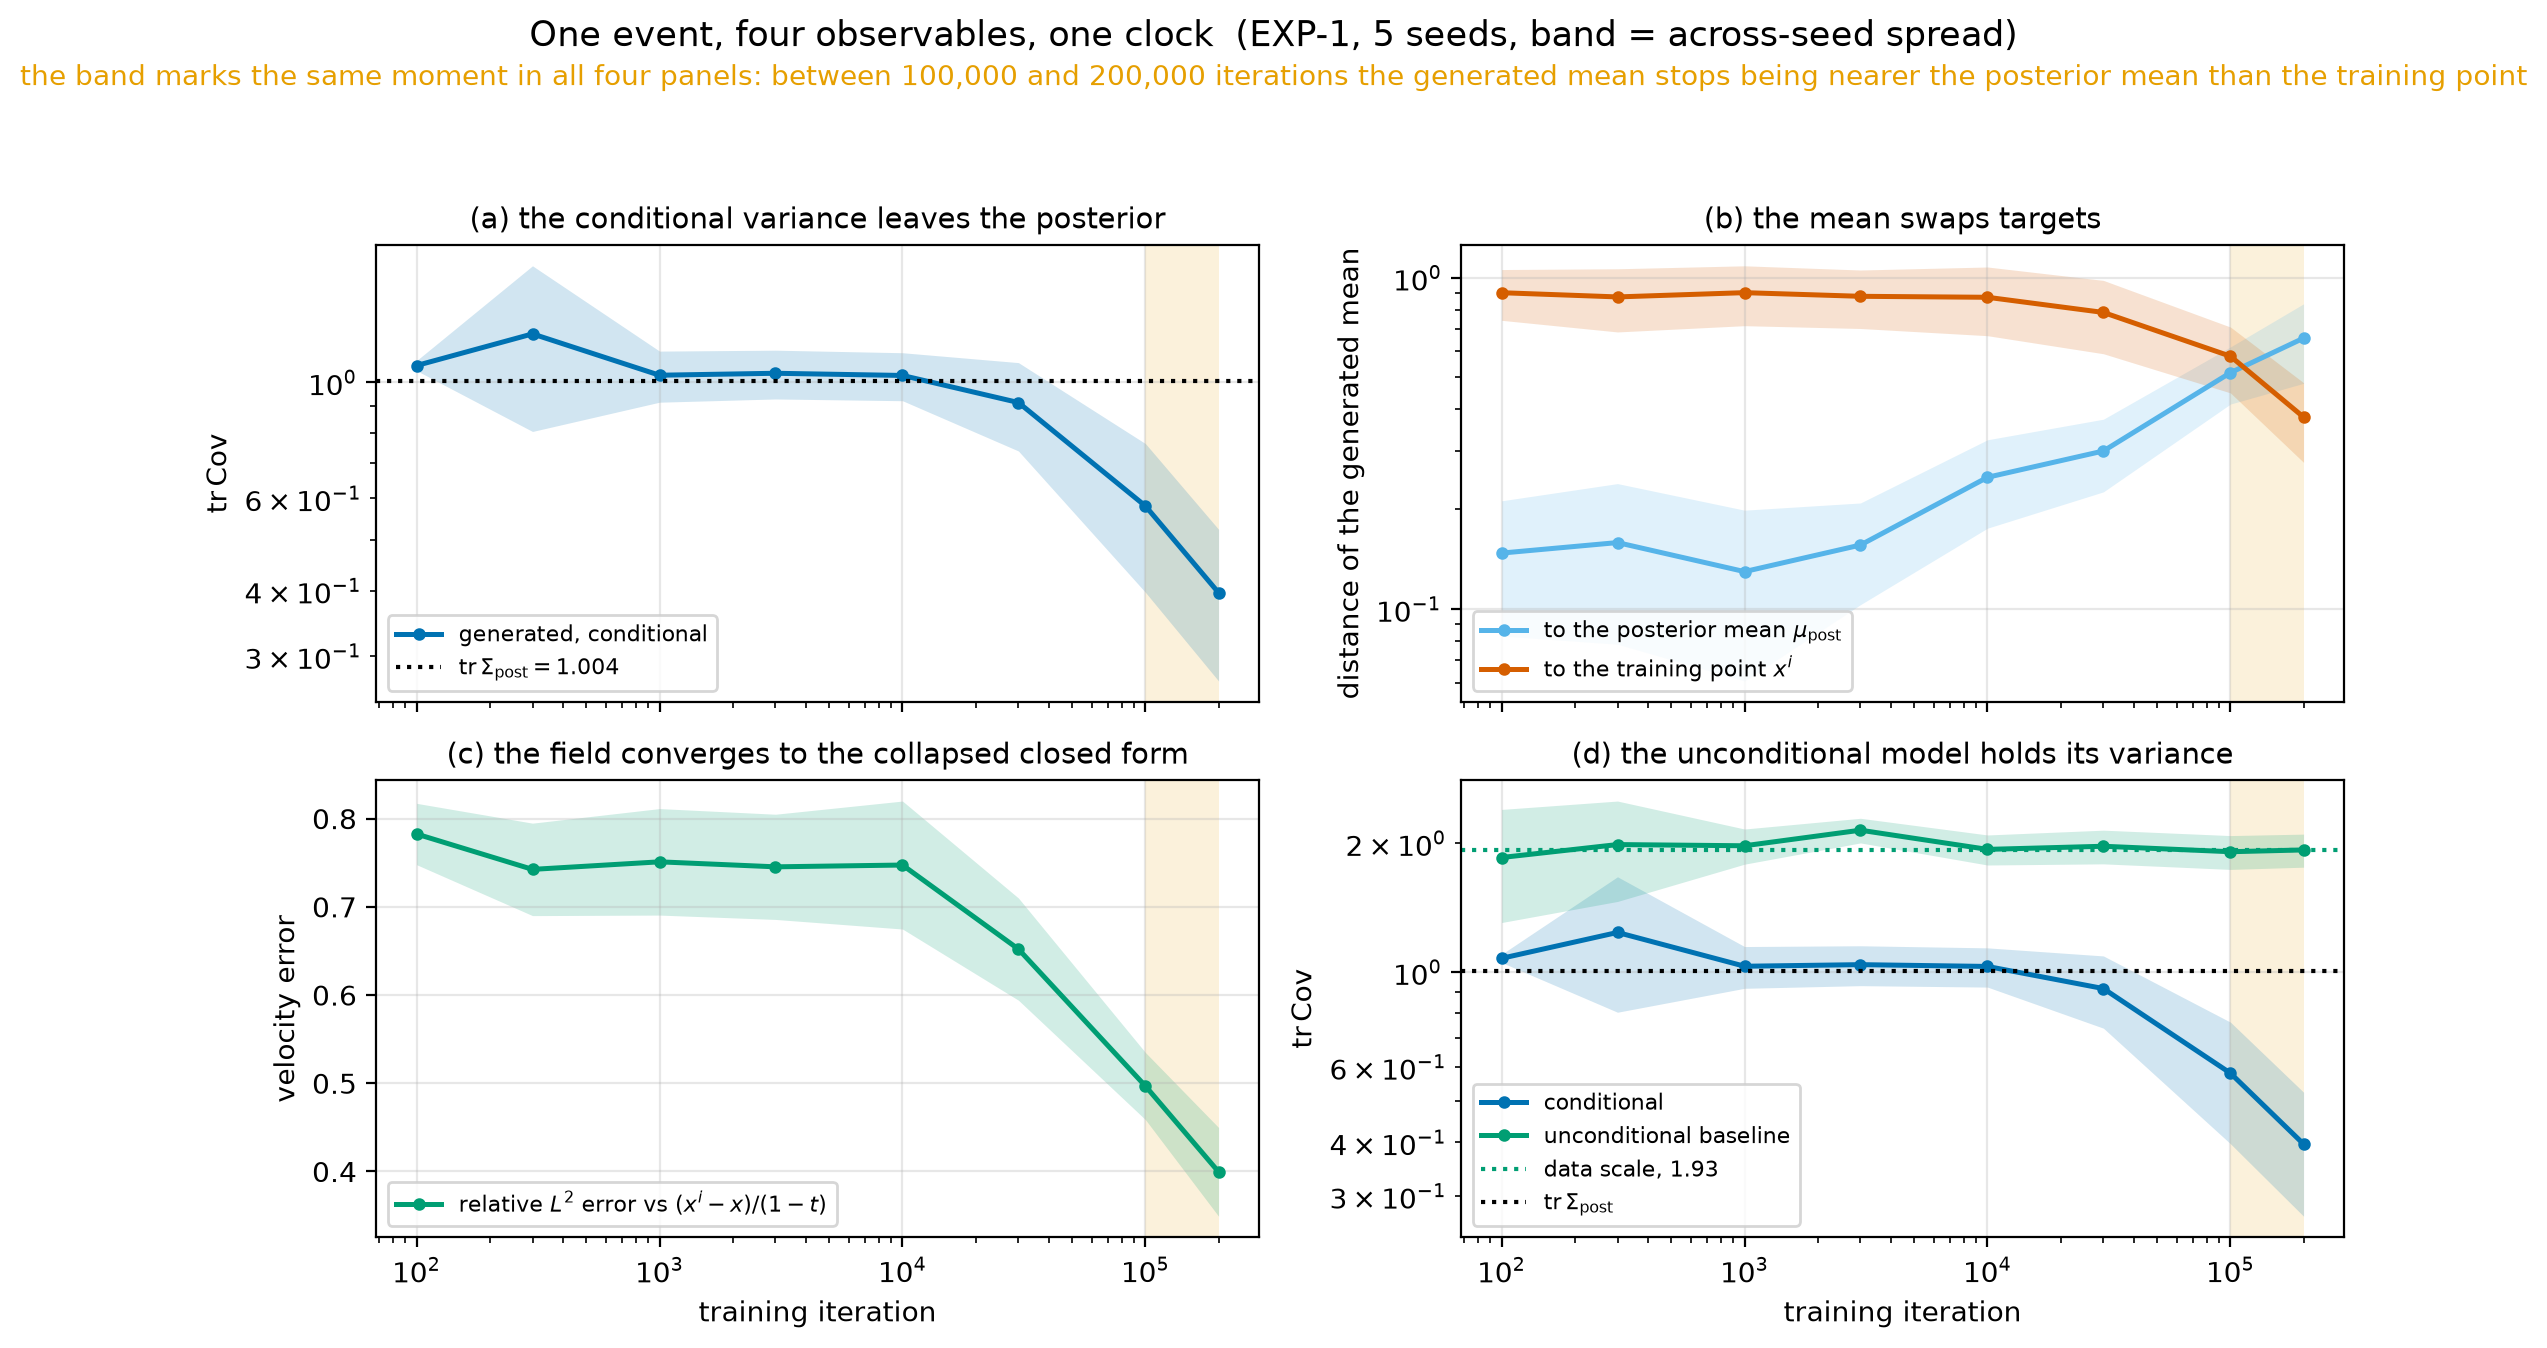
\includegraphics[width=\textwidth]{fig_p1p4.png}
\caption{The four exact-theory observables (P1--P4) on one clock, five seeds, band
$=$ across-seed spread. \textbf{(a)} the conditional variance sits on
$\tr\Sigmapost$---the sampler is calibrated---and then leaves it.
\textbf{(b)} the generated mean's distance to $\mu_{\mathrm{post}}$ rises while its
distance to the training point $x^i$ falls, and the two cross: before the crossing
the model is answering the inverse problem, after it the model is returning a
memorised image. \textbf{(c)} the velocity field's relative error against the
collapsed closed form $(x^i-x)/(1-t)$ falls. \textbf{(d)} the unconditional baseline
holds data-scale variance ($1.93$) throughout while the conditional falls away, which
is Corollary~\ref{cor:distinction}: the contrast is not memorising versus not, but
\emph{which} empirical measure is memorised. The shaded band is the same interval in
all four panels---the two checkpoints bracketing the crossing in (b)---and nothing
here turns at a different time.}
\label{fig:p1p4}
\end{figure}

This subsection collects the floats referenced from Section~\ref{sec:experiments}.
Table~\ref{tab:p7kernel} gives the full P7 kernel reference and
Table~\ref{tab:dagger} the velocity-field match, with the sample-space verification
in Figure~\ref{fig:kernel}. For EXP-1, Figure~\ref{fig:p1p4} plots all four observables on one clock,
Figure~\ref{fig:collapse2d} shows the
$d{=}2$ endpoint in sample space, Figure~\ref{fig:extended} the extended
cosine-schedule run, and Figure~\ref{fig:memratio} the memorisation ratio;
Figures~\ref{fig:adv-trace}--\ref{fig:adv-mean} cover the adversarial pairing and
Table~\ref{tab:p7i} the interpolant-noise contrast. For EXP-2/EXP-3,
Figure~\ref{fig:exp2curves} gives the mode-coverage and MMD curves,
Figure~\ref{fig:exp23qual} the qualitative GMM collapse,
Figure~\ref{fig:exp3curve} the quantitative MNIST curves, and
Figures~\ref{fig:exp3prog}--\ref{fig:exp3cifar} the MNIST and CIFAR-10 completion
grids.

\begin{table}[htb]
\centering\small
\begin{tabular}{lcccccc}
\toprule
$h$ & $\Covh$ (Thm~\ref{thm:endpoint}) & $\Sigmapost$ & generated $\tr\Cov$ &
\textbf{ratio-to-kernel} & ratio-to-post & $n_{\mathrm{eff}}$/200\\
\midrule
0.01 & 0.583 & 1.018 & $0.673\pm0.187$ & $1.308\pm0.376^{\dagger}$ & 0.66 & 3.5\\
0.05 & 0.921 & 1.018 & $0.926\pm0.169$ & $\mathbf{1.002\pm0.050}$ & 0.91 & 13.6\\
0.10 & 1.004 & 1.018 & $1.001\pm0.173$ & $\mathbf{0.994\pm0.039}$ & 0.98 & 26.0\\
0.50 & 1.281 & 1.018 & $1.294\pm0.166$ & $\mathbf{1.011\pm0.022}$ & 1.27 & 101.5\\
\bottomrule
\end{tabular}
\caption{P7 kernel reference, 5 seeds. For every $h\ge0.05$ the generated variance
tracks the exact kernel target $\Covh$ to within seed noise
(ratio-to-kernel $\approx1.00$, std $\le0.05$)---a verification of the \emph{endpoint
law}, stronger than a velocity-field check. $^{\dagger}$At $h{=}0.01$ ($n_{\mathrm{eff}}
\approx3.5$, single-atom regime) $\Covh$ is near-degenerate for many conditions, so the
per-condition ratio is unstable and high; the ratio of mean traces $0.673/0.583{=}1.15$
is closer to $1$.}
\label{tab:p7kernel}
\end{table}



\begin{figure}[htb]
\centering
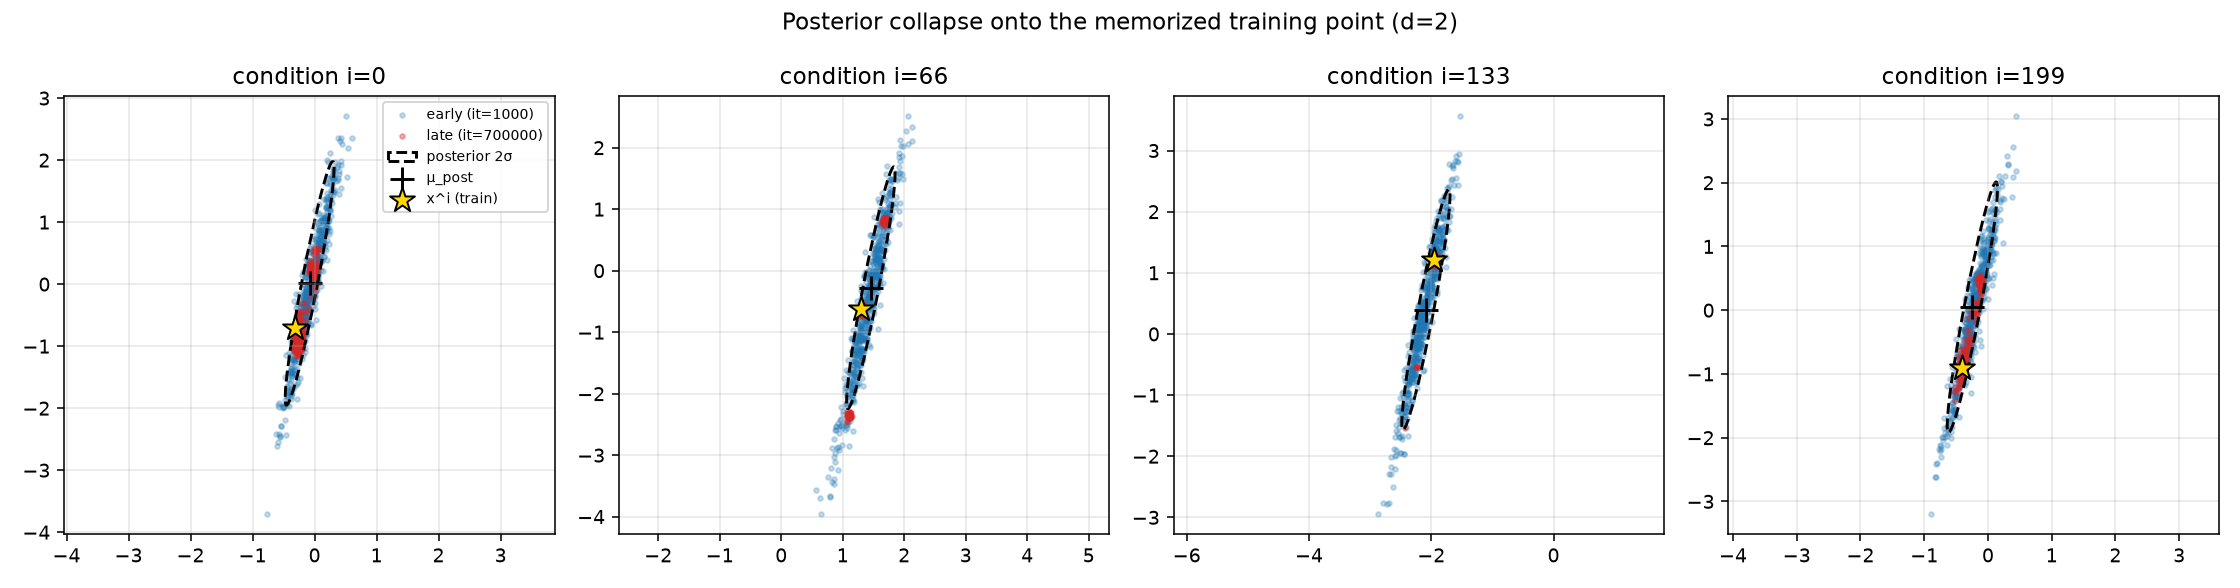
\includegraphics[width=0.95\textwidth]{fig_collapse2d.png}
\caption{Qualitative $d{=}2$ collapse (seed 0, cosine-schedule run at
$1{\times}10^6$ iterations): the sample cloud that initially fills the posterior
ellipse (blue, early, $10^3$ iterations) contracts onto the memorised training point
(red, late) for four conditions $y^i$. Because the late cloud is one to four orders
of magnitude tighter than the posterior scale, each panel carries an inset zoomed to
a fixed $\pm0.4$ window around $x^i$, annotated with that condition's $\tr\Cov$. The
collapse is not uniform across conditions at this budget---$i{=}133$ is essentially a
delta ($\tr\Cov=5.8\times10^{-5}$) while $i{=}0$ and $i{=}199$ retain a visible
residual spread ($8.4\times10^{-2}$, still $\sim12\times$ below
$\tr\Sigmapost$)---which is the optimisation-paced behaviour of
Section~\ref{sec:limitations}, not a failure of Proposition~\ref{prop:collapse}.}
\label{fig:collapse2d}
\end{figure}

\begin{figure}[htb]
\centering
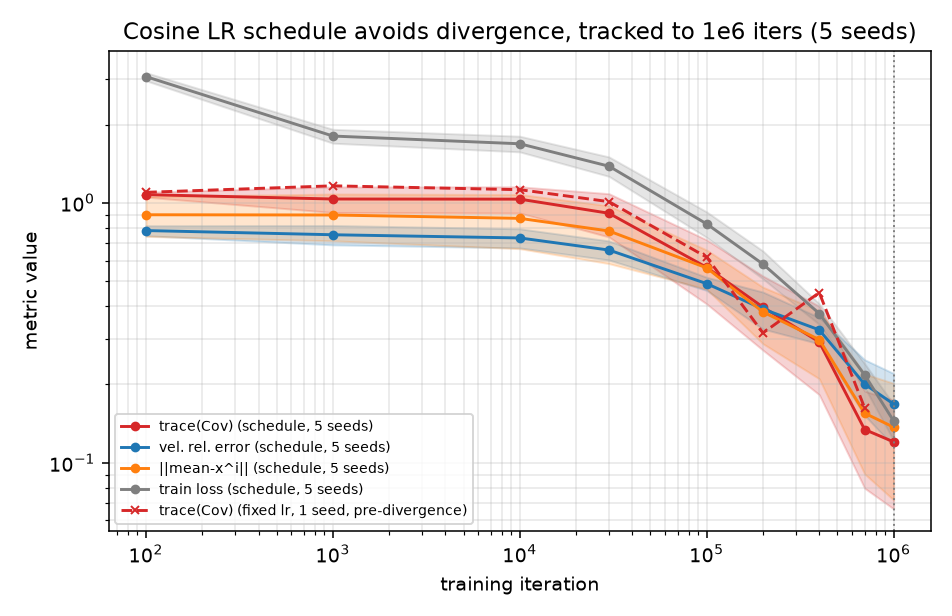
\includegraphics[width=0.85\textwidth]{fig_extended_schedule.png}
\caption{Extended training with a cosine learning-rate schedule (5 seeds,
error bars over seeds) tracks all the way to $10^6$ iterations without ever
diverging, unlike the fixed-lr single seed (dashed), which is cut off at its
last pre-divergence checkpoint. On the same seed, the schedule also reaches a
lower $\tr\Cov$ than the fixed-lr run at the matching $7\times10^5$ checkpoint
($0.128$ vs.\ $0.162$); the 5-seed mean at $1\times10^6$ carries enough
between-seed spread that it should be read mainly as evidence of stability, not
as a precise depth estimate (see main text). $\tr\Cov$, velocity error,
$\|\text{mean}-x^i\|$, and the training loss all decrease together throughout,
identifying P1--P3 as one phenomenon driven by $\text{loss}\to0$ (the exact
minimiser has loss $0$).}
\label{fig:extended}
\end{figure}

\begin{figure}[htb]
\centering
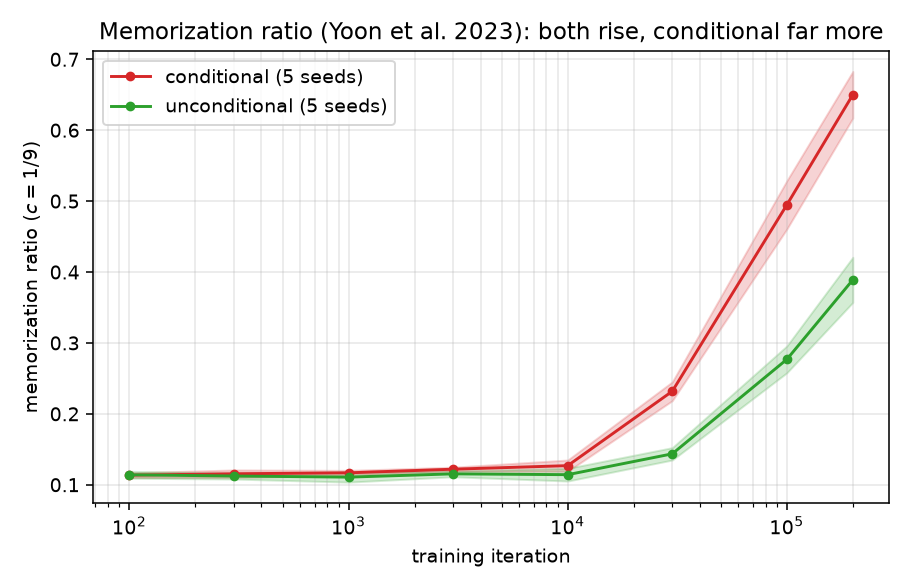
\includegraphics[width=0.72\textwidth]{fig_memorization_ratio.png}
\caption{Memorisation ratio (5 seeds each) for the same conditional and
unconditional EXP-1 runs as Figure~\ref{fig:p1p4}. Both rise from the common
$\approx0.11$ baseline of a well-calibrated sampler; the conditional ratio rises
higher ($0.650\pm0.033$ at $2\times10^5$) than the unconditional one
($0.389\pm0.032$), consistent with single-atom vs.\ full-empirical-measure
memorisation (Corollary~\ref{cor:distinction}).}
\label{fig:memratio}
\end{figure}

\begin{figure}[htb]
\centering
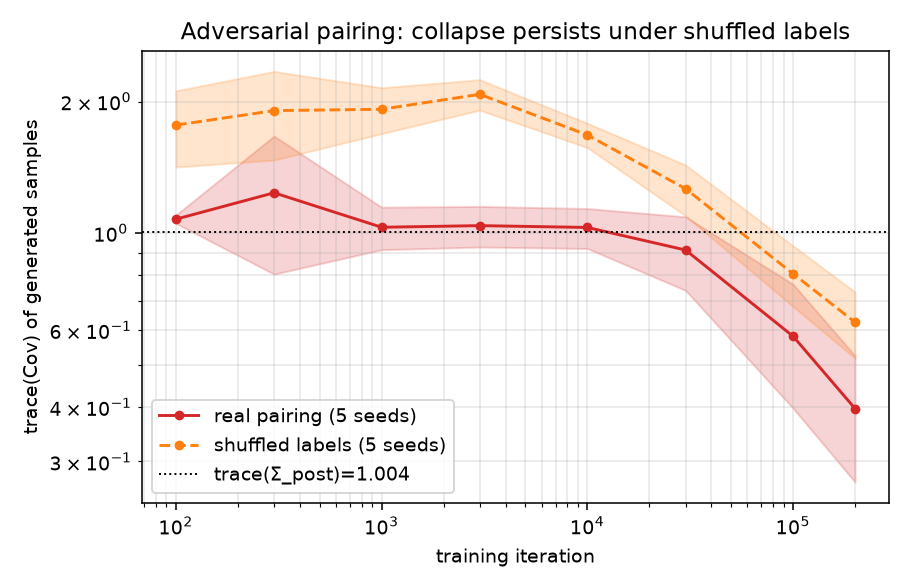
\includegraphics[width=0.72\textwidth]{fig_adv_trace_cov.png}
\caption{$\tr\Cov$ under the real EXP-1 pairing (5 seeds, as in Fig.~\ref{fig:p1p4})
vs.\ the same architecture and schedule trained on $Y$ randomly permuted relative to
$X$ (5 seeds). Both collapse monotonically well below $\tr\Sigmapost$; the shuffled
run lags the real pairing at $2\times10^5$ iterations ($0.625\pm0.108$ vs.\
$0.396\pm0.127$)---an optimisation-gap difference, not a failure of
Proposition~\ref{prop:collapse}, whose population target is $0$ either way.}
\label{fig:adv-trace}
\end{figure}

\begin{figure}[htb]
\centering
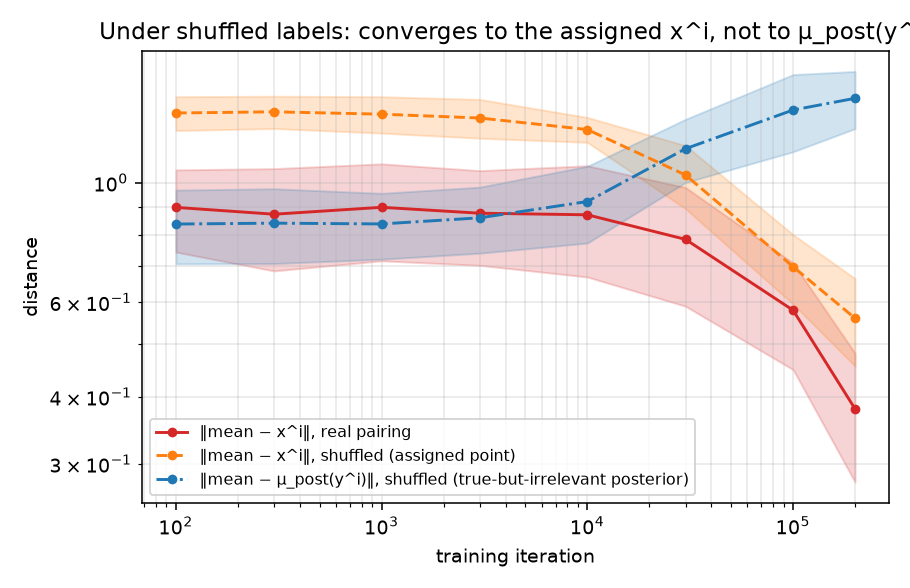
\includegraphics[width=0.72\textwidth]{fig_adv_mean_targets.png}
\caption{Under shuffled labels, the generated mean converges to the \emph{assigned}
training point $x^i$ ($\|\text{mean}-x^i\|:1.35\pm0.10\to0.559\pm0.104$) while moving
\emph{away} from the true analytic posterior mean of that $y^i$
($\|\text{mean}-\mu_{\mathrm{post}}(y^i)\|:0.84\pm0.13\to1.437\pm0.176$)---the two
curves cross between $10^4$ and $3\times10^4$ iterations. Under the real pairing the
corresponding gap is far smaller ($\|\text{mean}-\mu_{\mathrm{post}}\|=0.656\pm0.177$
at $2\times10^5$, Table~\ref{tab:exp1}), since there $x^i$ and $\mu_{\mathrm{post}}(y^i)$
are close by construction.}
\label{fig:adv-mean}
\end{figure}

\begin{table}[htb]
\centering\small
\begin{tabular}{lccc}
\toprule
$h$ & rel.\ error vs.\ \textbf{kernel} \eqref{eq:kernel-field} & rel.\ error vs.\ ($\star$) & TV of atom mixture\\
\midrule
0.01 & $\mathbf{0.318\pm0.030}$ & $0.599\pm0.104$ & $0.31\pm0.18$\\
0.05 & $\mathbf{0.195\pm0.019}$ & $0.683\pm0.103$ & $0.22\pm0.02$\\
0.10 & $\mathbf{0.162\pm0.021}$ & $0.703\pm0.092$ & $0.16\pm0.04$\\
0.50 & $\mathbf{0.164\pm0.025}$ & $0.791\pm0.070$ & $0.16\pm0.02$\\
\bottomrule
\end{tabular}
\caption{Velocity-field match (5 seeds). $v_\theta$ is $2$--$4\times$ closer to the
kernel field than to the collapsed field at every $h$. Assigning generated samples to
the nearest atom recovers the weights $p_i^{(h)}\propto K_h$ with total variation
$0.16$--$0.31$. At $h{=}0.5$ the generated variance $1.29$ \emph{overshoots}
$\Sigmapost{=}1.02$, matching the $+h^2\|J\|_F^2$ term of Proposition~\ref{prop:expansion}
($\|J\|_F^2=0.4031$, exact).}
\label{tab:dagger}
\end{table}

\begin{figure}[htb]
\centering
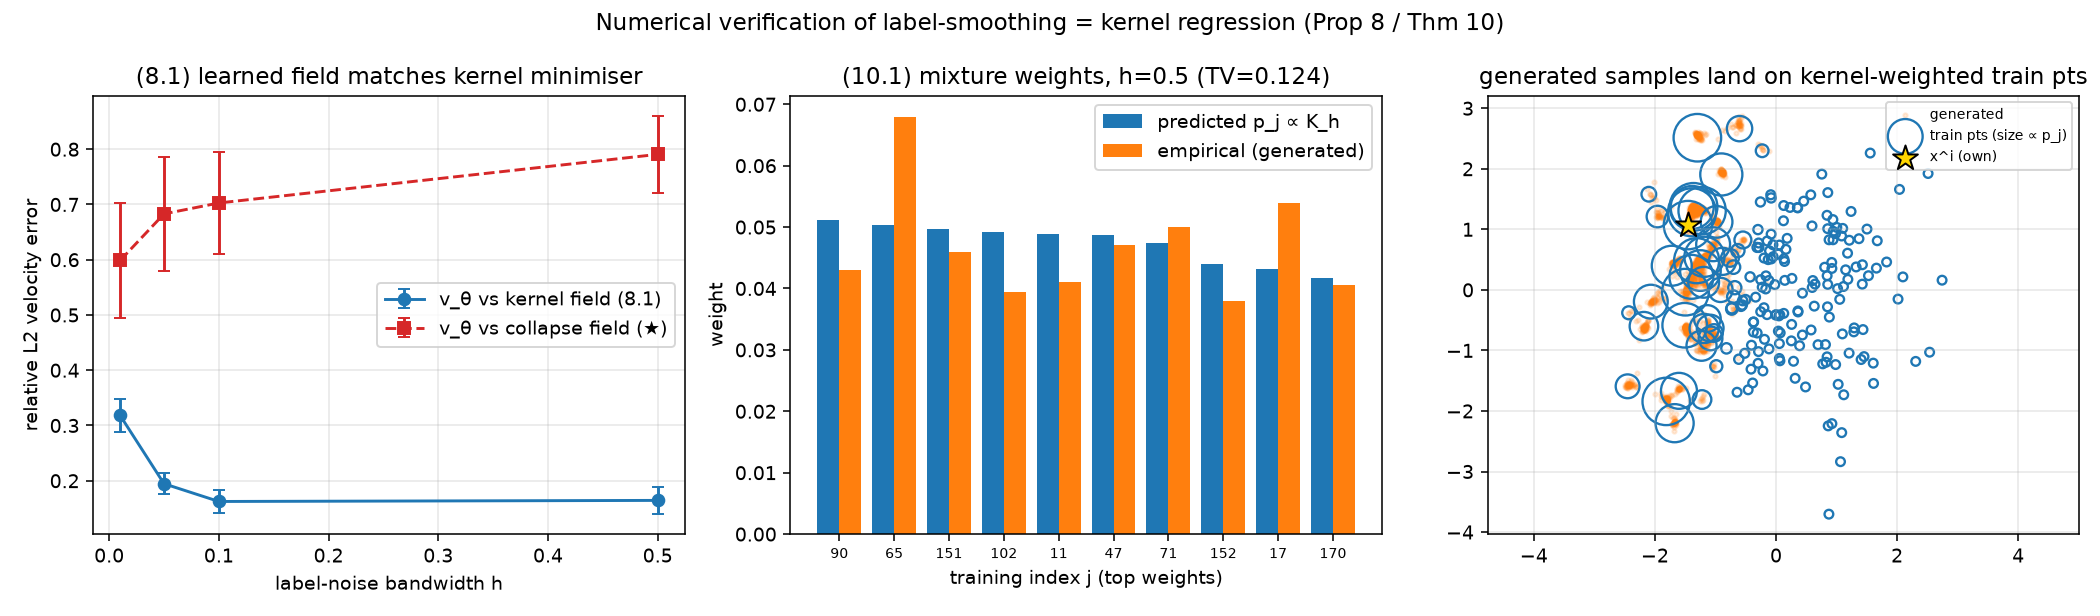
\includegraphics[width=0.95\textwidth]{fig_kernel_verify.png}
\caption{Kernel-theory verification: the learned field matches the kernel minimiser
\eqref{eq:kernel-field} (left); the predicted atom weights $p_i^{(h)}\propto K_h$ match
the empirical nearest-atom assignment (centre); and, for one condition $y$, generated
samples (orange) land on the training points weighted most heavily by the kernel
(blue circles, radius $\propto p_i^{(h)}$), confirming Theorem~\ref{thm:endpoint}'s
mixture-over-atoms endpoint law directly in sample space (right). The right panel is
at $h{=}0.5$, where the query's own atom $x^i$ (gold star) is only one of
$n_{\mathrm{eff}}\approx102$ contributors and therefore carries no special weight---the
opposite of the $h{\to}0$ regime of Corollary~\ref{cor:zerobw}. The panel headings
carry equation numbers from the development notes rather than this paper's: ``(8.1)''
is \eqref{eq:kernel-field} and ``(10.1)'' is Theorem~\ref{thm:endpoint}. The plot
cannot be regenerated with corrected labels because it reads the $p7y$ checkpoints,
which were not retained (see the reproducibility statement).}
\label{fig:kernel}
\end{figure}

\begin{table}[htb]
\centering\small
\begin{tabular}{lcc}
\toprule
interpolant $\sigma$ & 0.1 & 0.3\\
\midrule
$\tr\Cov$, old target $X_1-X_0$ (2 seeds) & $0.372\pm0.140$ & $0.429\pm0.121$\\
$\tr\Cov$, corrected target \eqref{eq:c2target} (5 seeds) & $\mathbf{0.367\pm0.146}$ & $\mathbf{0.383\pm0.131}$\\
$\|\text{mean}-\mu_{\mathrm{post}}\|$, corrected target (5 seeds) & 0.649 & 0.646\\
\bottomrule
\end{tabular}
\caption{Interpolant-noise contrast. Correcting the target leaves the result unchanged
within seed noise---a confirmation of Proposition~\ref{prop:prop17}(c), not a failure.}
\label{tab:p7i}
\end{table}

\begin{figure}[htb]
\centering
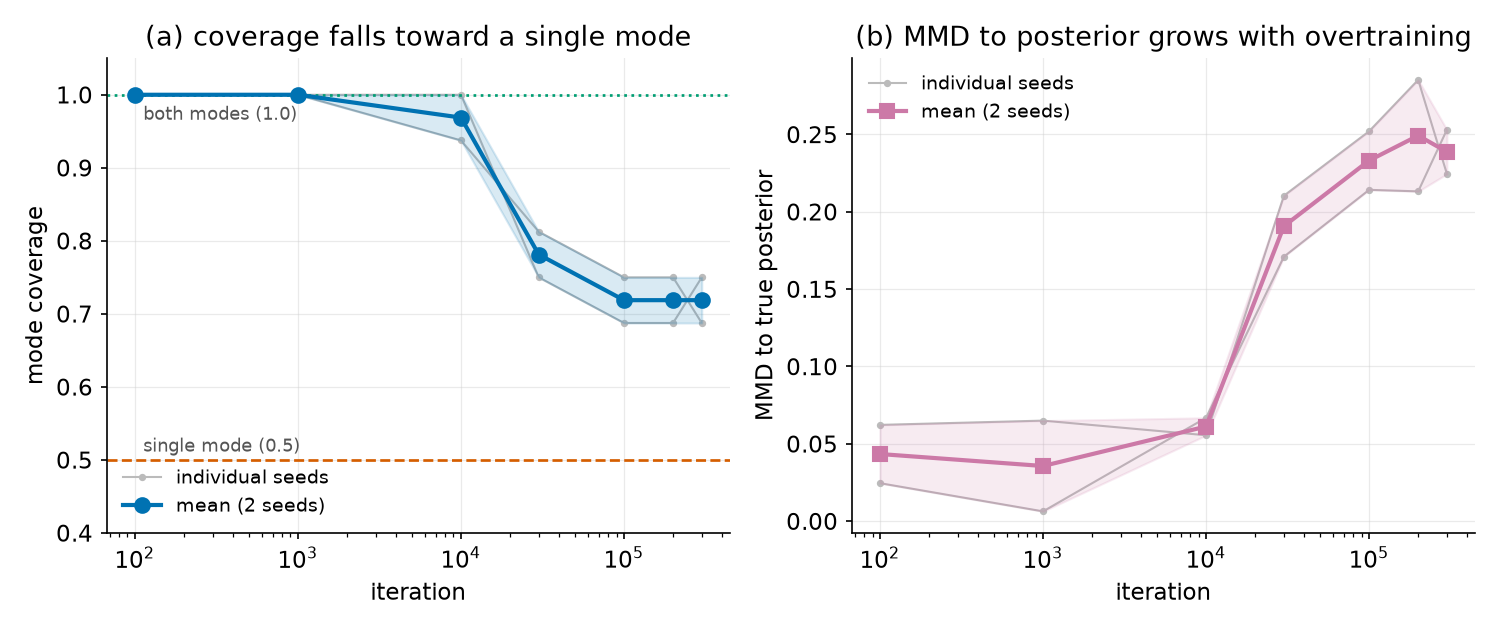
\includegraphics[width=0.92\textwidth]{fig_exp2_curves.png}
\caption{EXP-2 (GMM), mean of 2 seeds with per-seed traces and a $\pm$std band.
\textbf{(a)} Mode coverage holds at $1.0$ (both posterior modes) until $\sim\!10^4$
iterations, then falls toward the single-mode line $0.5$. \textbf{(b)} The MMD to the
true bimodal posterior is near zero in the calibrated phase and grows as overtraining
concentrates the samples on one mode. Onset matches EXP-1.}
\label{fig:exp2curves}
\end{figure}

\begin{figure}[htb]
\centering
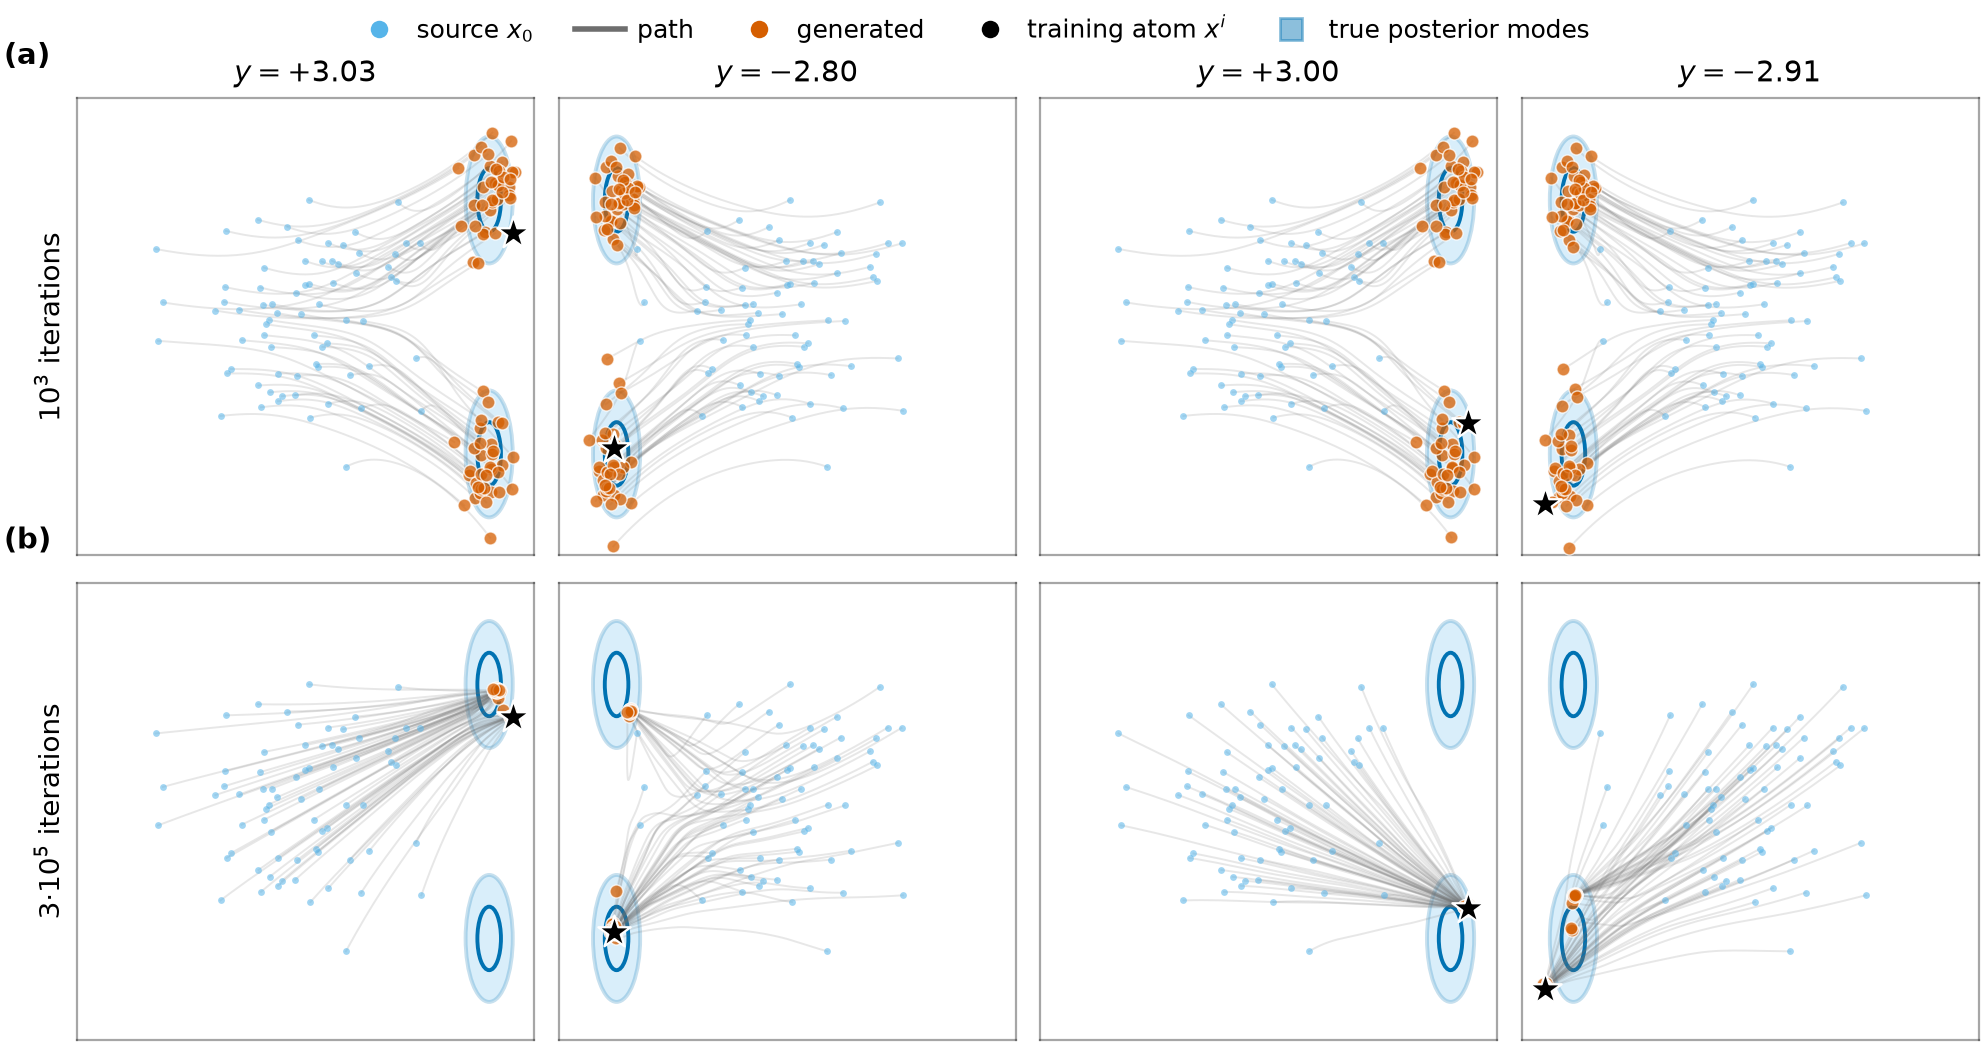
\includegraphics[width=0.95\textwidth]{fig_exp2_portrait.png}
\caption{EXP-2 in trajectory space (seed 0), on four of the $N{=}100$ conditions, one
per column. The ellipses are the two modes of the bimodal analytic posterior and the
star is the memorised $x^i$. \textbf{(a)}~At $10^3$ iterations the $70$ source draws
(blue) are carried to \emph{both} modes. \textbf{(b)}~At $3{\times}10^5$ iterations the
same draws fan into a single point: assigning late samples to their nearest posterior
mode, the share landing in the $x^i$-containing mode is $0.999$, $0.766$, $0.990$ and
$1.000$ for the four conditions (versus $0.37$--$0.55$ at iteration $10^3$). The one
condition that retains $23\%$ of its mass on the abandoned mode shows that this is an
optimisation-paced process (Section~\ref{sec:limitations}), consistent with the
aggregate mode coverage of Section~\ref{sec:exp23} settling at $0.72$ rather than
at the single-mode value $0.5$. Produced by \texttt{scripts/make\_exp2\_portrait.py},
which recomputes the four shares from $20000$ draws and asserts that they agree with
the values quoted here.}
\label{fig:exp23qual}
\end{figure}

\begin{figure}[htb]
\centering
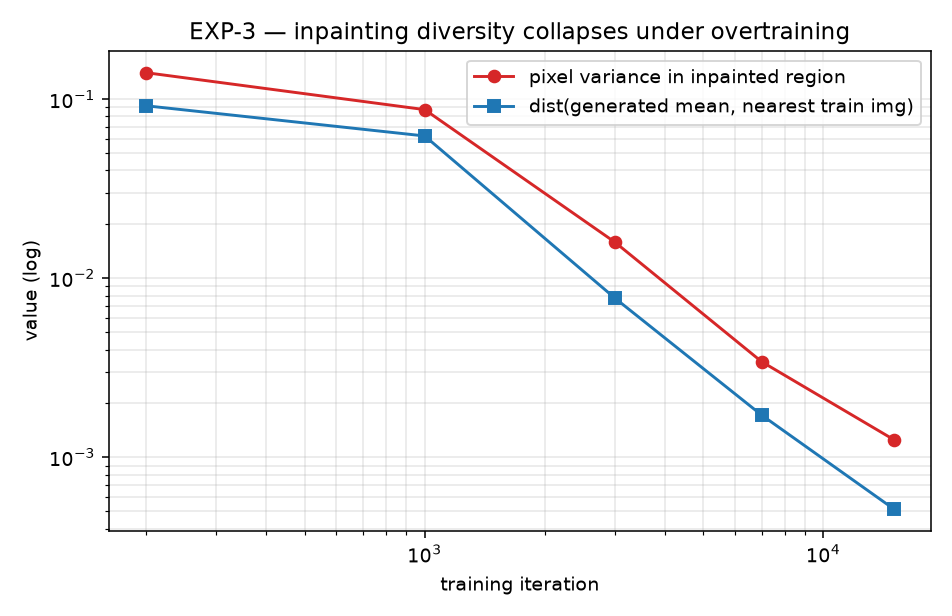
\includegraphics[width=0.62\textwidth]{fig_exp3_curve.png}
\caption{EXP-3 (MNIST inpainting), quantitative collapse, shown for seed 0 (whose
checkpoint schedule is the finest of the three; the 3-seed statistics at the shared
$15000$-iteration checkpoint are in the text). The inpaint-region pixel variance and
the distance to the nearest training image both fall by roughly two orders of
magnitude as the loss descends.}
\label{fig:exp3curve}
\end{figure}

\begin{figure}[htb]
\centering
\begin{subfigure}{0.5\textwidth}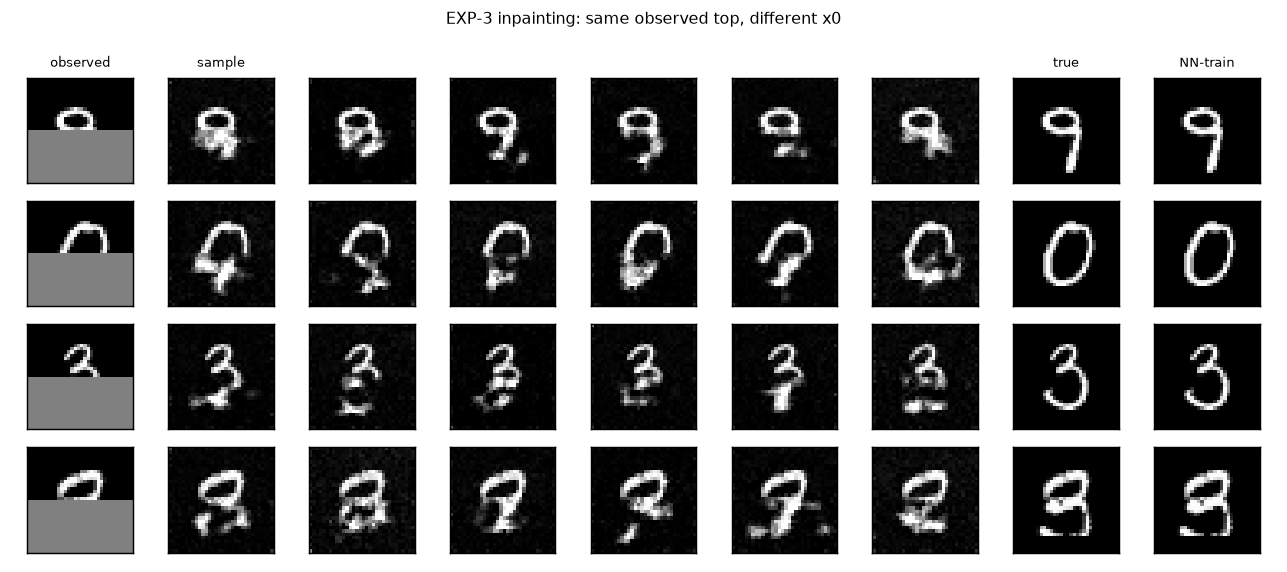
\includegraphics[width=\linewidth]{fig_exp3_grid200.png}
\caption{iter 200}\end{subfigure}\\[3pt]
\begin{subfigure}{0.5\textwidth}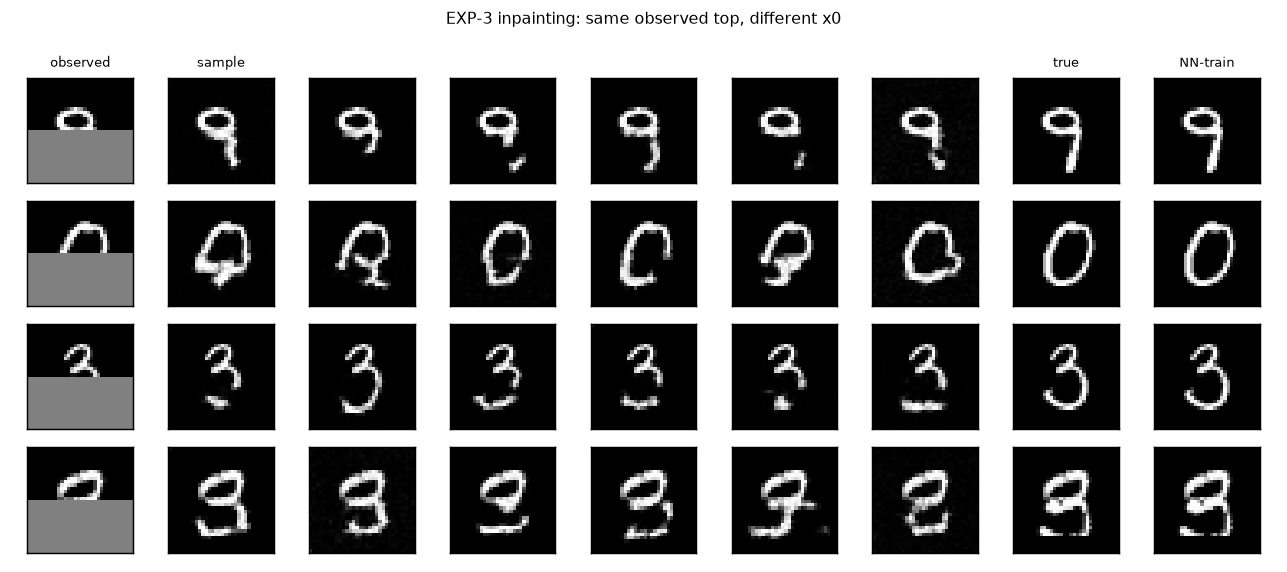
\includegraphics[width=\linewidth]{fig_exp3_grid1000.png}
\caption{iter 1000}\end{subfigure}\\[3pt]
\begin{subfigure}{0.5\textwidth}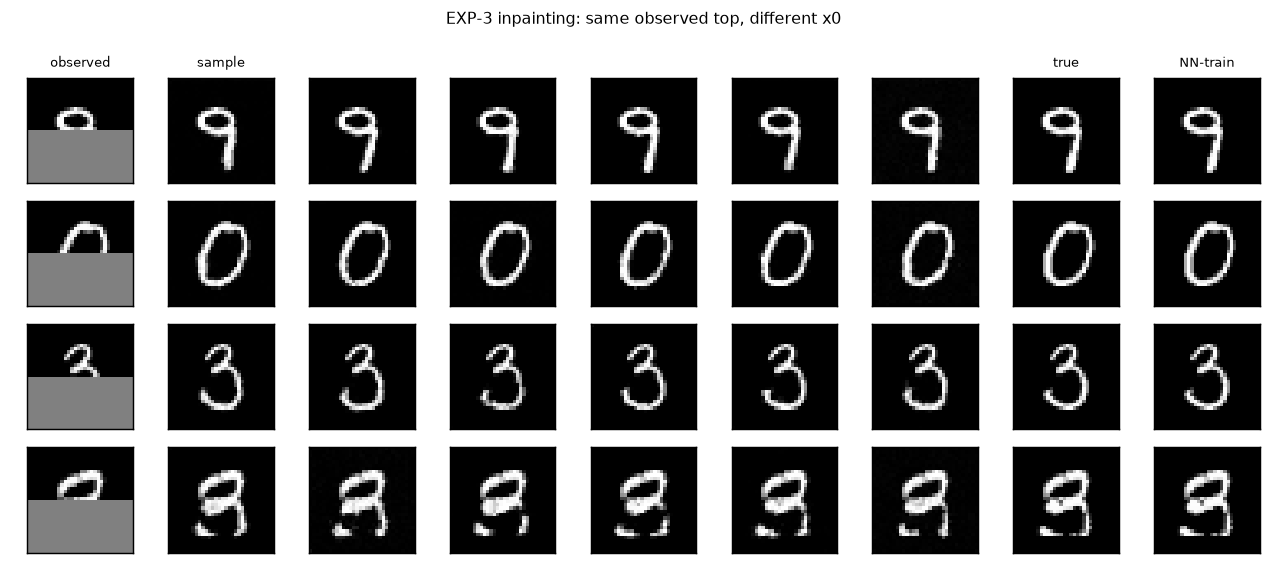
\includegraphics[width=\linewidth]{fig_exp3_grid3000.png}
\caption{iter 3000}\end{subfigure}\\[3pt]
\begin{subfigure}{0.5\textwidth}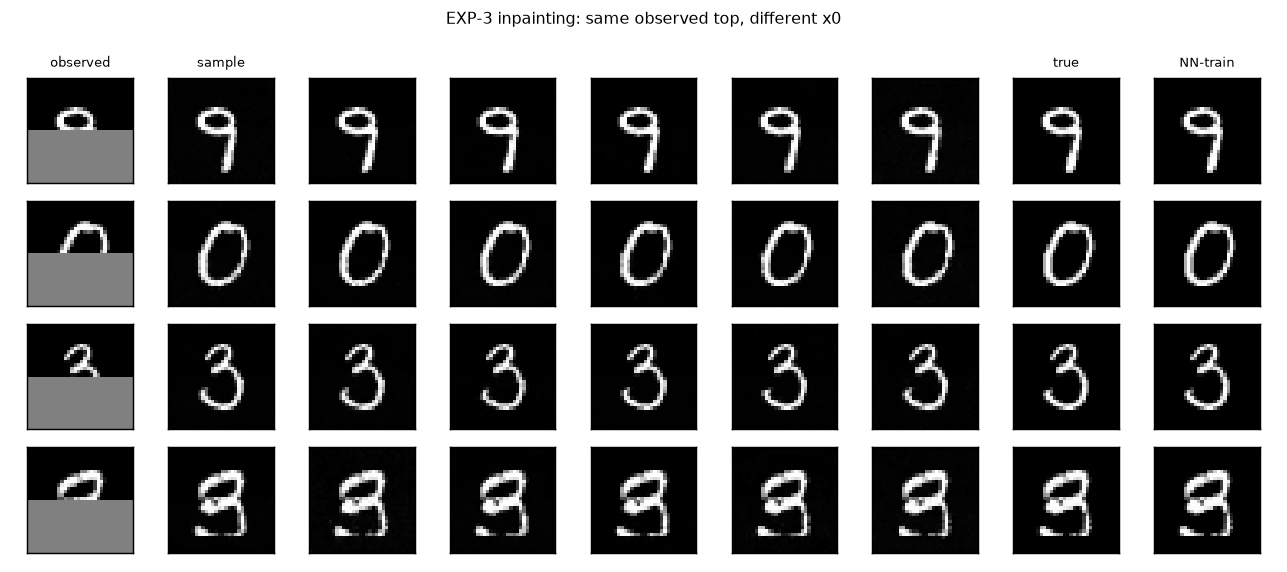
\includegraphics[width=\linewidth]{fig_exp3_grid7000.png}
\caption{iter 7000}\end{subfigure}\\[3pt]
\begin{subfigure}{0.5\textwidth}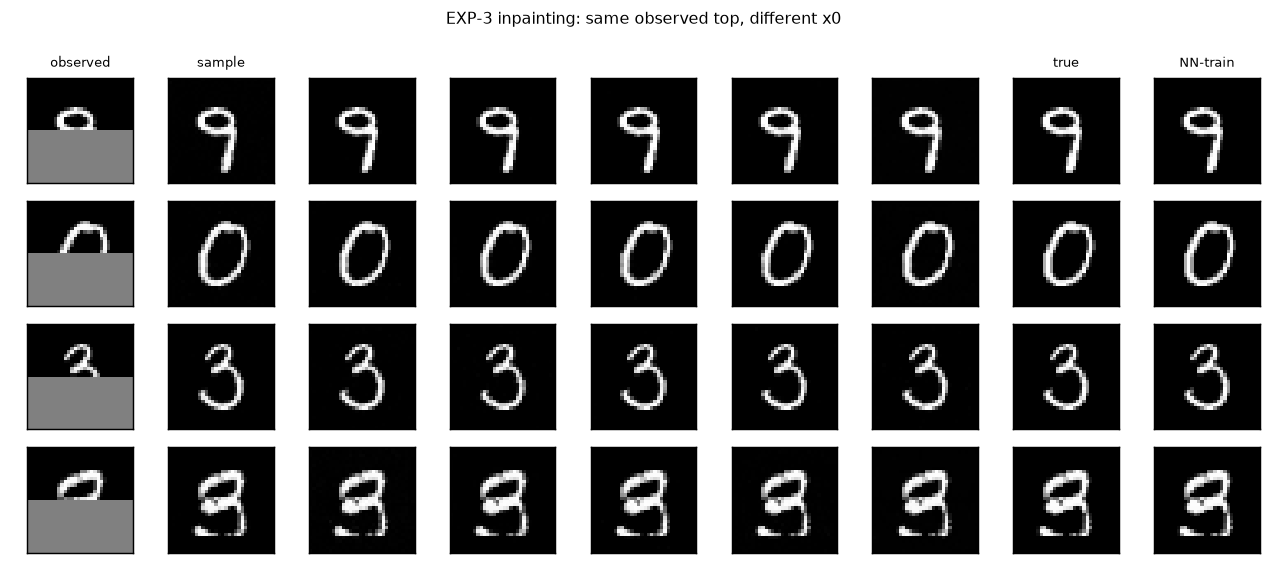
\includegraphics[width=\linewidth]{fig_exp3_grid15k.png}
\caption{iter 15000}\end{subfigure}
\caption{EXP-3 collapse trajectory (MNIST inpainting). Each grid shows completions of a
fixed masked digit from different source samples $x_0$. Early in training (iter 200) the
completions are diverse---a calibrated conditional sampler; as the loss descends they
sharpen progressively (iter 1000--7000) and, by iter 15000, are identical to one another
and equal to the nearest training image (inpaint-region pixel variance
$0.137\!\to\!0.0012$ averaged over 3 seeds, a $\sim\!100\times$ drop). This is the
same $\text{loss}\!\to\!0$-paced collapse as EXP-1, on real image data, and it
reproduces on CIFAR-10 too (Figure~\ref{fig:exp3cifar}).}
\label{fig:exp3prog}
\end{figure}
\begin{figure}[htb]
\centering
\begin{subfigure}{0.48\textwidth}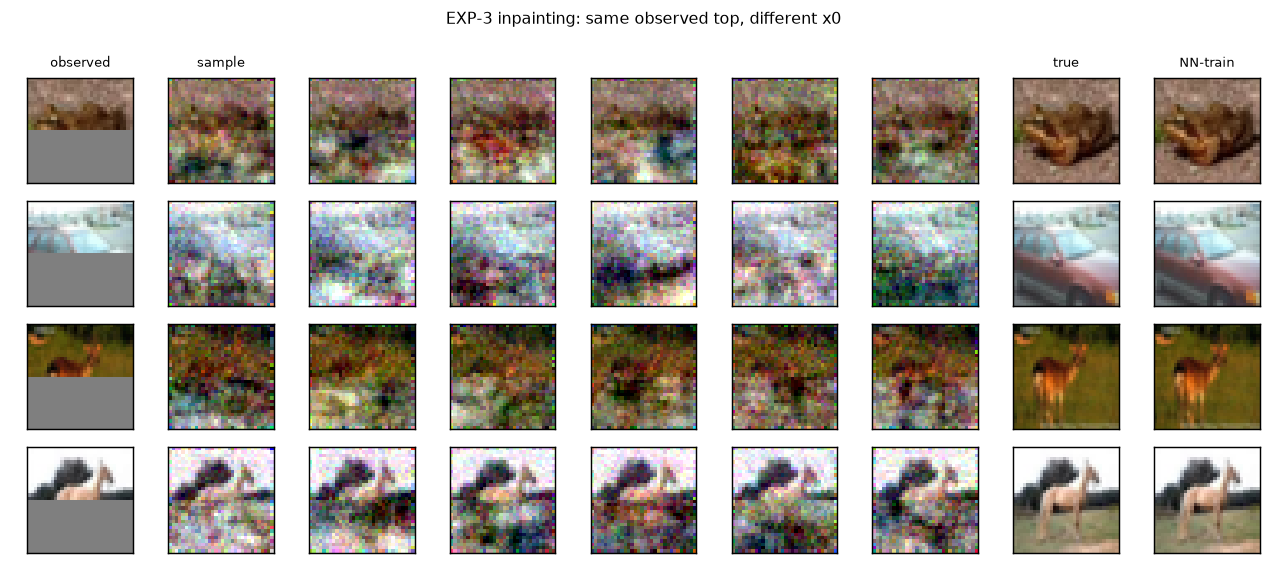
\includegraphics[width=\linewidth]{fig_exp3_cifar_grid200.png}
\caption{iter 200}\end{subfigure}\hfill
\begin{subfigure}{0.48\textwidth}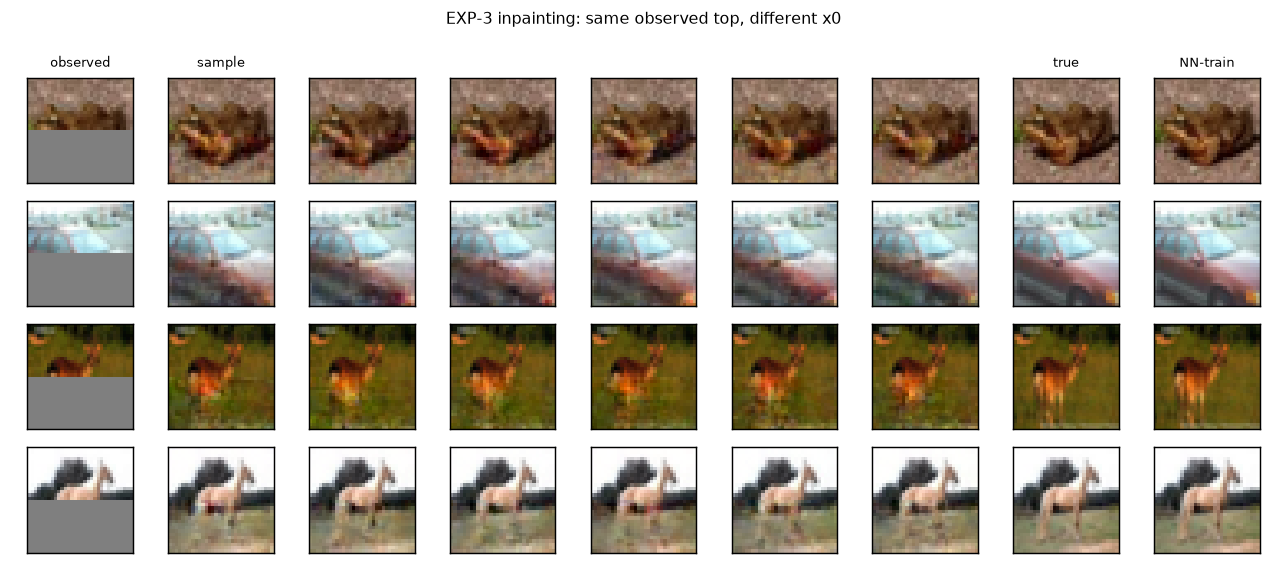
\includegraphics[width=\linewidth]{fig_exp3_cifar_grid15k.png}
\caption{iter 15000}\end{subfigure}
\caption{EXP-3 on CIFAR-10 (one seed), same protocol as Figure~\ref{fig:exp3prog}.
At iteration 200, completions of the masked bottom half are diverse and noisy; by
iteration 15000 they are visually identical to each other and closely match the
nearest training image (rightmost two columns), confirming the collapse mechanism is
not specific to MNIST's simplicity. The residual mismatch to that image is larger
here than on MNIST (nearest-image distance $0.0040$ vs.\ $0.00077$), consistent with
CIFAR-10's harder loss landscape at the same $15000$-iteration budget. The same
comparison for the DDPM runs, across label bandwidths, is Figure~\ref{fig:imagebandwidth}.}
\label{fig:exp3cifar}
\end{figure}

\begin{figure}[htb]
\centering
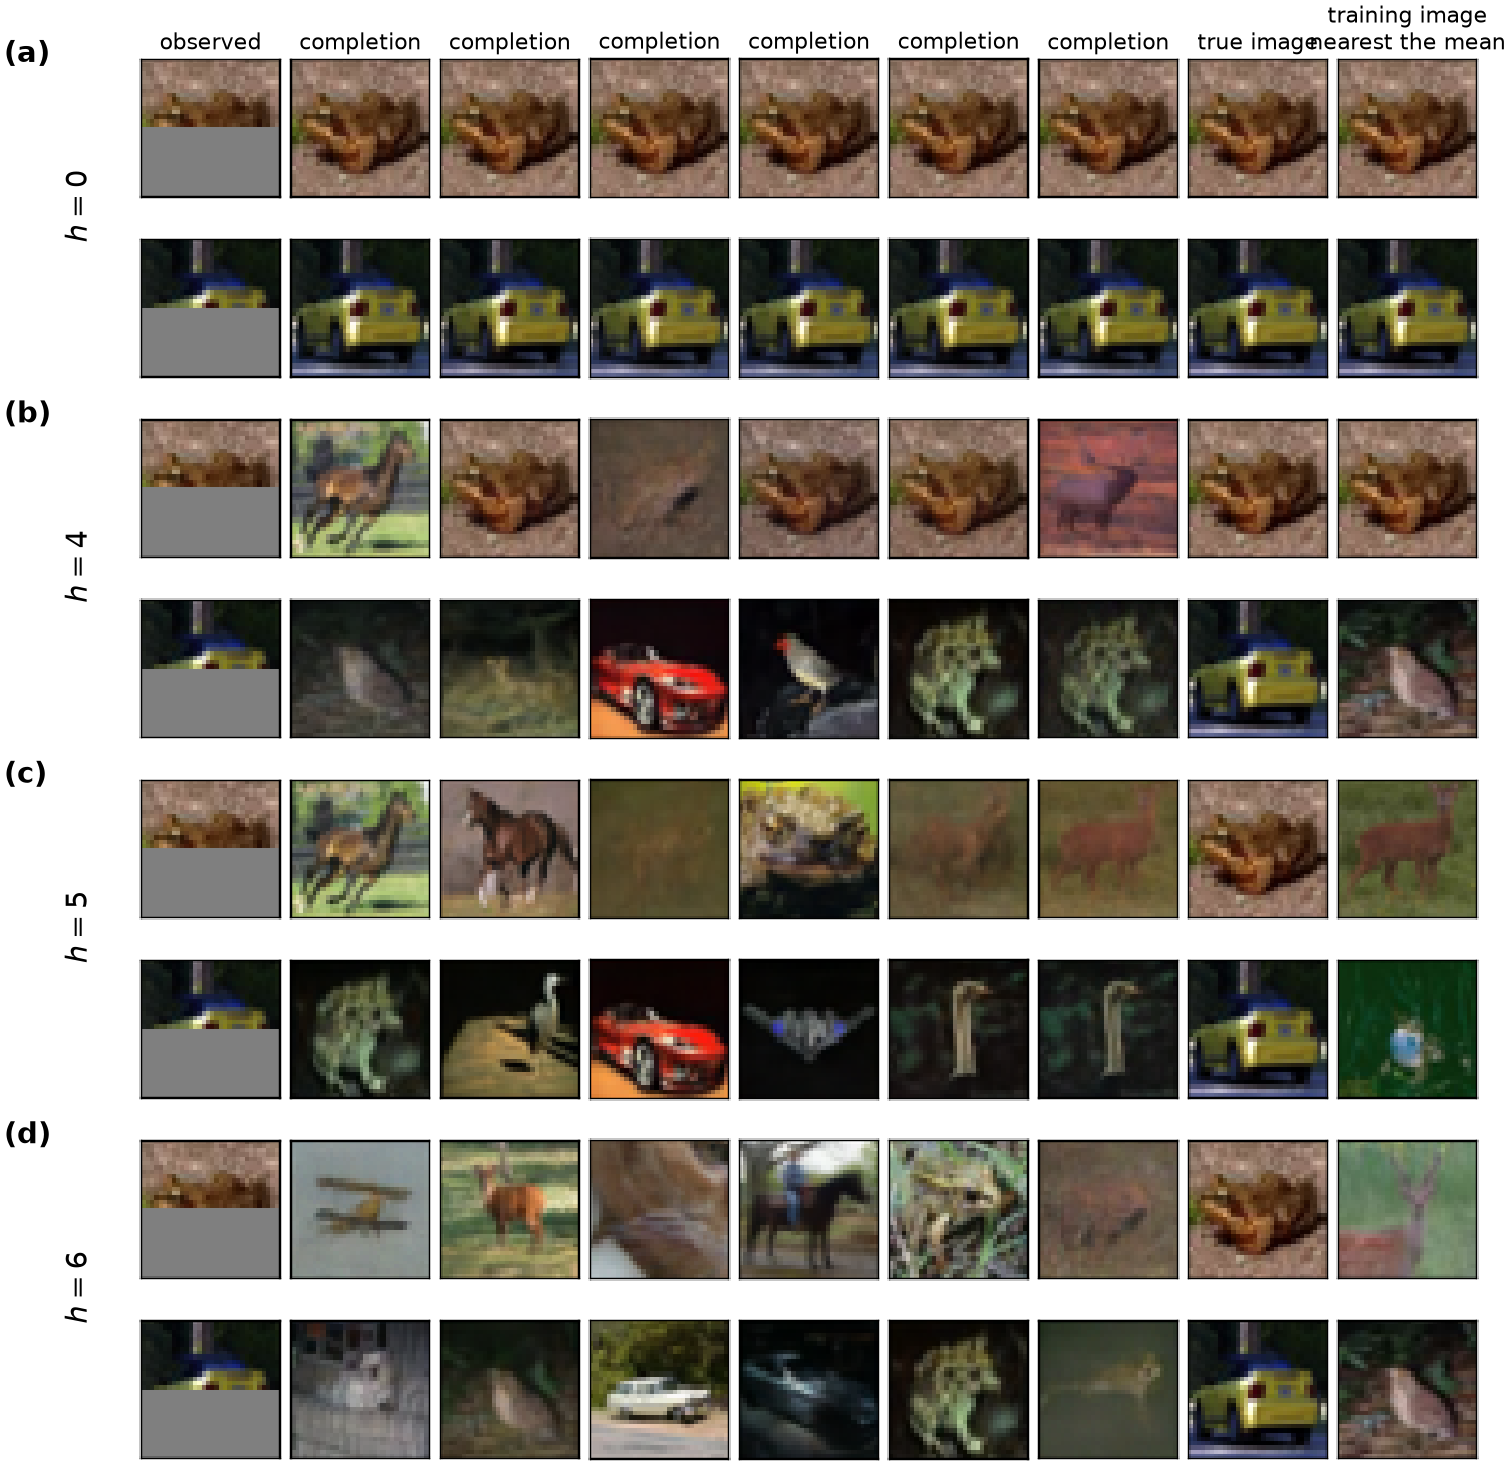
\includegraphics[width=0.9\textwidth]{fig_image_bandwidth.png}
\caption{Inpainting with the CIFAR-10 DDPM U-Net ($35.75$M parameters, $6{\times}10^4$
iterations) at four label bandwidths, on two of the four displayed conditions. Each row
is the observed top half, six completions of the masked bottom half from different source
draws $x_0$, the true image, and the training image nearest the mean completion.
\textbf{(a)}~$h{=}0$: all six completions are one image, the true one, on both
conditions (Proposition~\ref{prop:collapse}). \textbf{(b--d)}~$h{>}0$: the completions
differ from one another, but they do not become posterior draws. At $h{=}4$ three of the
six completions in the upper row still reproduce the true frog, and in the lower row none
reproduces the true car; at $h{=}5$ and $h{=}6$ none does in either row. The same
images, a galloping horse and a red car, recur across conditions and bandwidths, as a law
supported on training atoms predicts (Proposition~\ref{prop:atomicity}); the blurred
completions, which look like no training image, are the kind of off-atom mass
Section~\ref{sec:cifarddpm} quantifies. Cut from the sample grids the runs saved,
by \texttt{scripts/make\_image\_bandwidth\_figure.py}.}
\label{fig:imagebandwidth}
\end{figure}

\end{document}
